%&preamble

%Symbole

% Symbol: Pfeil zum Zurückspringen
\newcommand{\zurueck}{%
	\begin{tikzpicture}[scale=0.15]
%	\fill [gray!40] (0,0) circle [radius=1.5];
	\draw [thick, -{>[length=3pt, width=5pt]}] (-0.6,0.6) arc [start angle=-230, end angle=100, radius=1] -- ++(-0.1,0);
	\end{tikzpicture}
}

%Symbol: Werkzeug
\newcommand{\werkzeug}{%
	\begin{tikzpicture}[scale=0.1, rotate=45]
%	\filldraw [fill=white, draw=black] (3,0) circle [radius=4cm];
	\path [thick, fill=gray, draw=black] (3.5,0.5) -- (0,0.5) arc [start angle=90, end angle=270, radius=0.5] (0,-0.5) -- (3.5,-0.5) -- (3.8,0) -- (3.5,0.5);
	\path [thick,draw=black, fill=gray] (3.5,-0.5) ++(1,0.5) ++(206.57:1.118) arc (206.57:315:1.118) -- ++(-0.9,0) -- (3.8,0) ++ (0.7,0) ++(-206.57:1.118) arc (-206.57:-315:1.118) -- ++(-0.9,0) -- (3.8,0);
	\draw [very thick, gray] (3.5,-0.5) -- (3.8,0) -- (3.5,0.5);
	\fill [gray!50, rounded corners=1] (0.3,0.25) rectangle (3.2,0.3);
	\fill [gray!50, rounded corners=1] (0.3,-0.25) rectangle (3.2,-0.3);
	\end{tikzpicture}
}

%Symbol: Drucker
\newcommand{\drucker}{%
	\begin{tikzpicture}[scale=0.2]
		\draw (0.5,0.5) rectangle (1.5,1.8);
		\foreach \x in {1.2,1.4,1.6}	
		\draw (0.6,\x) -- (1.4,\x);
		\draw [rounded corners=0.5pt, fill=gray!80!black] (0,0) rectangle (2,1);
	\end{tikzpicture}
}

%Symbol: Video
\newcommand{\video}{%
	\begin{tikzpicture}[scale=0.2]
		\draw [rounded corners=3pt, fill=gray!20] (0,0) rectangle (3,2);
		\draw [fill=gray] (1,0.5) -- (1,1.5) -- (2,1) -- (1,0.5);
	\end{tikzpicture}
}

%Symbol: Präsentationsfolie
\newcommand{\folie}{%
	\begin{tikzpicture}[scale=0.17]
	\draw [rounded corners=1pt,thick] (0,0) rectangle (3,2);
	\draw [rounded corners=1pt,fill=gray!30] (0.3,0.3) rectangle (1.3,1.6);
	\draw [rounded corners=1pt,fill=gray!30] (1.7,0.3) rectangle (2.7,1.6);
	\draw [thick] (1.1,-0.4) -- (1.5,0) -- (1.9,-0.4);
	\draw [fill=gray] (-0.2,1.8) rectangle (3.2,2.1);
	\end{tikzpicture}
}

%Symbol: Internetlink
\newcommand{\wlan}{%
	\begin{tikzpicture}[scale=0.5]
		\fill[black] (1mm,1mm) circle [radius=1mm];
		\draw [ultra thick] (0.4,0) arc [start angle=0, end angle=90, radius=4mm];
		\draw [ultra thick] (0.6,0) arc [start angle=0, end angle=90, radius=6mm];
		\draw [ultra thick] (0.8,0) arc [start angle=0, end angle=90, radius=8mm];
	\end{tikzpicture}
}

%Symbol: Ausrufezeichen
\newcommand{\ausrufezeichen}{%
	\begin{tikzpicture}[scale=0.8]
	\fill[gray!70] (0,0) circle [radius=1mm];
	\fill[gray] (0,0.15) -- (0.05,0.6) -- (-0.25,0.7) -- (-0.1,0.15) -- (0,0.15);
	\fill[gray!50] (0.05,0.15) -- (0.1,0.6) -- (-0.2,0.7) -- (-0.05,0.15) -- (0.05,0.15);
	\end{tikzpicture}
}

%Symbol: Schaltplan
\newcommand{\schaltsym}{%
	\begin{tikzpicture}[scale=0.3,rotate=30]
		\filldraw [fill=white, draw=black] (0.2,0.25) circle [radius=1.3];
		\draw (0,0) rectangle (0.5,0.5);
		\draw (0,0.5) -- (0,1.2) (0,1) -- (-0.5,1);
		\filldraw [fill=white, draw=black] (0,1.2) circle [radius=0.1];
		\filldraw [fill=white, draw=black] (-0.5,1) circle [radius=0.1];
		\draw (0.5,0.5) -- (0.5,1) (0.5,0.7) -- (1,0.7) -- (1,0);
		\filldraw [fill=white, draw=black] (0.5,1) circle [radius=0.1];
		\filldraw [fill=white, draw=black] (1,0) circle [radius=0.1];
		%\draw (1,0.5) -- (1,1) (1,0.5) -- (1.5,0.5) -- (1.5,1);
		%\filldraw [fill=white, draw=black] (1,1) circle [radius=0.1];
		%\filldraw [fill=white, draw=black] (1.5,1) circle [radius=0.1];
		%\draw (1,0) -- (1.5,0) -- (1.5,-0.5);
		%\filldraw [fill=white, draw=black] (1.5,-0.5) circle [radius=0.1];
		\draw (0.5,0) -- (0.5,-0.5);
		\filldraw [fill=white, draw=black] (0.5,-0.5) circle [radius=0.1];
		\draw (0,0) -- (-0.5,0) (-0.5,0.5) -- (-0.5,-0.5);
		\filldraw [fill=white, draw=black] (-0.5,0.5) circle [radius=0.1];
		\filldraw [fill=white, draw=black] (-0.5,-0.5) circle [radius=0.1];
	\end{tikzpicture}
}

%Symbol: Arduino / Code

\newcommand{\codesym}{%
	\begin{tikzpicture}[scale=0.6]
		\filldraw [thick, fill=white, draw=black] (0,0) circle [radius=0.7];
		\draw [very thick] (-0.3,0) circle [radius=0.3];
		\draw [very thick] (0.3,0) circle [radius=0.3];
		%\draw [ultra thick] (-0.1,-0.2) -- (0.1,0.2);
		%\draw [ultra thick] (-0.1,0.2) -- (0.1,-0.2);
		\node at (-0.3,-0.1) {\bfseries -};
		\node at (0.3,0) {\bfseries +};
	\end{tikzpicture}	
}

%Symbol: Lupe für eigene Untersuchungen
\newcommand{\lupe}{%
	\begin{tikzpicture}[scale=0.25]%
%	\filldraw [fill=white, draw=black] (0.6,0.6) circle [radius=1.52];
	\shadedraw [ball color=gray!10, draw=black, thick, name path=kreis] (1,1) circle (0.5);
	\path [name path=mpursprung] (1,1) -- (0,0);
	\draw [name intersections={of=kreis and mpursprung, by=x}][thick] (x) -- (0,0);
	\end{tikzpicture}%
}

%Symbol: kleines i für Informationen
\newcommand{\infosym}{%
	\begin{tikzpicture}[scale=0.3]%
	\filldraw [fill=white, draw=black] (0,0) circle [radius=1];
	\node at (0,0) {\bfseries\LARGE i};
	\end{tikzpicture}%
}

%LED
\newcommand{\ledsym}[1][~]{%
	\begin{tikzpicture}[scale=0.7,baseline=-2mm]
	\fill [CadetBlue!70!green] (0,0) circle (0.25cm); %ursprünglich gray!50!white
	\fill [CadetBlue!70!green] (-0.25,0) rectangle (0.25,-0.3);
	\draw [thick, gray!50!white] (-0.1,-0.3) -- (-0.1,-0.4);
	\draw [thick, gray!50!white] (0.1,-0.3) -- (0.1,-0.5);
	\node at (0,-0.05) {\sffamily \bfseries #1};
	\end{tikzpicture}
}

%kleiner Widerstand
\newcommand{\resistorsym}{%
	\begin{tikzpicture}[scale=0.05,baseline=-1mm]
	\shade [top color=lightgray, bottom color=gray] (-5,0.8) rectangle (10,1.2);
	\shade [top color=LightSkyBlue, bottom color=NavyBlue] (0,0) -- (5,0) arc [start angle=-135, end angle=135, radius=1.414] -- (0,2) arc [start angle=45, end angle=315, radius=1.414];
	\fill [orange] (0,0) rectangle ++(0.5,2);
	\fill [green] (1,0) rectangle ++(0.5,2);
	\fill [black] (2,0) rectangle ++(0.5,2);
	\fill [black] (3,0) rectangle ++(0.5,2);
	\fill [brown] (4.5,0) rectangle ++(0.5,2);
	\end{tikzpicture}
}



% Open Roberta Lab - Menü
\newcommand{\nepomenu}{%
	\begin{tikzpicture}[scale=0.3]
		\draw [thick,gray, rounded corners=0.2mm] (0,0) rectangle (1,1.4);
		\foreach \y in {0.2, 0.4, ..., 1.2} {
			\draw [thick, gray] (0.2,\y) -- (0.8,\y);
		}
	\end{tikzpicture}
}

% Open Roberta Lab - export
\newcommand{\nepoexport}{%
	\begin{tikzpicture}[scale=0.3]
	\fill [black] (0,0) rectangle (1,0.3);
	\draw [thick] (0.03,0.3) -- (0.35,0.7);
	\draw [thick] (0.97,0.3) -- (0.65,0.7);
	\draw [thick] (0.35, 0.5) -- ++(0.15,-0.1) -- ++(0,0.6) ++(0,-0.6) ++(0.15,0.1) -- ++(-0.15,-0.1)  ;
	\end{tikzpicture}
}

% Open Roberta Lab - Quellcode
\newcommand{\nepoquellcode}{%
	\begin{tikzpicture}
		\fill[gray!40, rounded corners] (0,0) rectangle (0.5,0.4);
		\draw [thick] (0.22,0.1) -- (0.1,0.2) -- (0.22,0.3);
		\draw [thick] (0.28,0.1) -- (0.4,0.2) -- (0.28,0.3);
	\end{tikzpicture}
}
%\newcommand{\nepoquellcode}{\tcbox[size=fbox,box align = base,colback=gray!20, colframe=gray,nobeforeafter]{\bfseries\texttt{<>}}}

% Open Roberta Lab - Hilfe
\newcommand{\nepohilfe}{%
	\begin{tikzpicture}
	\fill[gray!40, rounded corners] (0,0) rectangle (0.5,0.4) node at (0.25,0.2) {\color{black}\sffamily\bfseries ?};
	\end{tikzpicture}
}

% Open Roberta Lab - Expertenblöcke
\newcommand{\nepoexpert}{%
	\begin{tikzpicture}
	\draw [scale=0.5, thick] (0.5,1) -- (0.39,0.65) -- (0.02,0.65) -- (0.32,0.44) -- (0.21,0.1) --  (0.5,0.31) -- (0.79,0.1) -- (0.68,0.44) -- (0.98,0.65) -- (0.61,0.65) -- (0.5,1);
	\node at (0.75,0.25) {\bfseries\sffamily 2};
	\end{tikzpicture}
}

%%%%%%%%%%%%% Arduino / Überschrift %%%%%%%%%%%%%%%%%%
\newcommand{\ardusym}{}
\def\ardusym(#1,#2) {%
	\draw (#1,#2) rectangle ++(14,7) ++(-12.5,-3.5) node [above, right] {\parbox{11cm}{\Huge \sffamily \textbf{Wahlpflichtfach Arduino} \\ \Large Skript zur Einführung in Elektronik und Programmierung mit dem Arduino \\ \\
	}};
	% Linke Seite
	\draw (#1,#2) ++(0,2) -- ++(-0.3,0) ++(0.3,0) node [right] {\scriptsize\sffamily 3V3};
	\draw (#1,#2) ++(0,3.5) -- ++(-0.3,0) ++(0.3,0) node [right] {\scriptsize\sffamily 5V};
	\draw (#1,#2) ++(0,5) -- ++(-0.3,0) ++(0.3,0) node [right] {\scriptsize\sffamily VIN};
	% Rechte Seite
	\draw (#1,#2) ++(14,3.5) -- ++(0.3,0) ++(-0.3,0) node [left] {\scriptsize\sffamily GND};
	% Obere Seite
	\foreach \x in {0, ..., 13} {%
		\draw (#1,#2) ++(2,7) ++(0.78*\x,0) -- ++(0,0.3) ++(0,-0.3) node [below] {\sffamily \scriptsize D\x};
	}
	% Untere Seite
	\draw (#1,#2) ++(2,0) -- ++(0,-0.3) ++(0,0.3) node [above] {\scriptsize\sffamily RESET};
	\draw (#1,#2) ++(3.5,0) -- ++(0,-0.3) ++(0,0.3) node [above] {\scriptsize\sffamily RESET2};
	\draw (#1,#2) ++(5,0) -- ++(0,-0.3) ++(0,0.3) node [above] {\scriptsize\sffamily AREF};
	\draw (#1,#2) ++(6.5,0) -- ++(0,-0.3) ++(0,0.3) node [above] {\scriptsize\sffamily ioref};
	\foreach \x in {0, ..., 5} {
		\draw (#1,#2) ++(2+0.78*8,0) ++(0.78*\x,0) -- ++(0,-0.3) ++(0,0.3) node [above] {\scriptsize\sffamily A\x};
	}
}
% Befehle mit tcolorbox-Paket
\newcommand{\button}[1]{\tcbox[size=fbox,box align = base,colback=gray!20, colframe=gray,nobeforeafter]{\texttt{#1}}}
%\newtcolorbox{zsfg}{before=\medskip, enhanced, interior style={top color=CadetBlue!80!green, bottom color=DarkCyan!70!DarkGreen}, coltext=white, colframe=white, after=\medskip}
%\newtcolorbox{zsfg}[1]{before=\medskip, breakable, enhanced, colback=CadetBlue!70!green, coltext=black, colframe=DarkCyan!70!DarkGreen, fonttitle=\bfseries, after=\medskip, title=#1, attach title to upper, after title={\medskip}}
\newtcolorbox{zsfg}[1]{before=\medskip, breakable, enhanced, colback=CadetBlue!70!green, coltext=black, frame style={left color=CadetBlue!75!green, right color=DarkCyan!70!DarkGreen},fonttitle=\bfseries, after=\medskip, title=#1}
\newtcolorbox{ziel}{before=\medskip, breakable, sharp corners=all, enhanced, frame style={left color=CadetBlue!70!green, right color=DarkCyan!70!DarkGreen}, after=\medskip}


%	Definition der Aufgabenumgebung
\newcounter{aufgabennummer}[chapter]	%durch das optionale Argument wird der section-Counter als übergeordneter Zähler festgelegt,
% sodass die aufgabennummer auf null gesetzt wird, wenn section erhöht wird
\newenvironment{aufgabe}{%
	\medbreak %
	\textbf{\sffamily Aufgabe}%
	\stepcounter{aufgabennummer}%Counter beginnt immer bei 0, also vor der Ausgabe hochzählen
%	\ifnum \value{section}>0 %
%		~\textbf{\sffamily\thesection.\theaufgabennummer}%
%	\else ~\textbf{\sffamily\theaufgabennummer}%
%	\fi% falls die Aufgabe in einem Abschnitt steht, wird dieser zur Nummerierung herangezogen
	~\textbf{\sffamily\theaufgabennummer}:~%
}{ %
	\par\medskip %

}

\newenvironment{aufgabe*}{%
	\medbreak %
	\textbf{\sffamily Aufgabe}%
	:~%
}{ %
	\par\medskip %
	
}

\newcounter{projektnummer}[chapter]
\newenvironment{projekt}[1][\unskip]{%
	\begin{tcolorbox}[breakable,before=\medbreak, enhanced, frame hidden, interior hidden, borderline west={1mm}{-4mm}{CadetBlue!70!green}, top=0mm,bottom=0mm,boxsep=0mm, left=0mm, right=0mm, after=\medskip]
	\textbf{\sffamily Projekt}%
	\stepcounter{projektnummer}% 
%	\ifnum \value{section}>0 %
%	~\textbf{\sffamily\thesection.\theprojektnummer}%
%	\else ~\textbf{\sffamily\theprojektnummer}%
%	\fi% falls die Aufgabe in einem Abschnitt steht, wird dieser zur Nummerierung herangezogen
	~\textbf{\sffamily\theprojektnummer}:~%
	\textbf{#1} \smallbreak%
}{ %
	\end{tcolorbox}
	\par\medskip %
	 %
}

\newenvironment{projekt*}[1][\unskip]{%
	\begin{tcolorbox}[breakable,before=\medbreak, enhanced, frame hidden, interior hidden, borderline west={1mm}{-4mm}{CadetBlue!70!green}, top=0mm,bottom=0mm,boxsep=0mm, left=0mm, right=0mm, after=\medskip]
		\textbf{\sffamily Projekt}%
		:~%
		\textbf{#1} \smallbreak%
	}{ %
	\end{tcolorbox}
	\par\medskip %
	%
}

\newenvironment{links}{%
	\begin{tcolorbox}[before=\bigbreak, enhanced, frame hidden, colback=gray!20, after=\medskip]
	\wlan \textbf{\sffamily Motivationsquellen}%
	\begin{itemize}[noitemsep, itemindent=0pt, leftmargin=5mm, label=>]
}{%
	\end{itemize}
	\end{tcolorbox}
	\par\medskip %
	%
}

\newenvironment{projektueberblick}{%
	\begin{tcolorbox}[before=\bigbreak, enhanced, frame hidden, colback=CadetBlue!70!green, after=\medskip]
	\textbf{\sffamily Projekte in diesem Kapitel:}%
	\setlength{\columnsep}{2cm}
	\begin{multicols}{2}
	\begin{itemize}[noitemsep, itemindent=0pt, leftmargin=5mm, label=>]
	}{%
	\end{itemize}
	\end{multicols}
	\end{tcolorbox}
	\par\medskip %
	%
}

\newenvironment{recherche}[1]{%
	\medbreak
	\lupe ~ \textbf{Recherche:~#1}
	\par
}{%
	\par \medskip
}

\definecolor{blueviolet}{RGB}{138,43,226}
\definecolor{turquoise1}{RGB}{0,245,255}
\definecolor{chocolate}{RGB}{210,105,30}
\definecolor{olivedrab}{RGB}{107,142,35}
\definecolor{khaki}{RGB}{240,230,140}
\definecolor{deeppink}{RGB}{255,20,147}
\definecolor{navyblue}{RGB}{0,0,128}
\definecolor{aquamarine}{RGB}{127,255,212}
\definecolor{sandybrown}{RGB}{244,164,96}
\definecolor{seagreen}{RGB}{46,139,87}
\definecolor{coral}{RGB}{255,127,80}
\definecolor{darkorchid}{RGB}{153,50,204}
\definecolor{seagreen3}{RGB}{67,205,128}
\definecolor{dodgerblue}{RGB}{30,144,255}
\definecolor{burlywood4}{RGB}{139,115,85}

%\newenvironment{wichtig}[1][]{%
%	\begin{mdframed}[%
%		backgroundcolor={gray!15}, hidealllines=true,
%		skipabove=0.7\baselineskip, skipbelow=0.7\baselineskip,
%		splitbottomskip=2pt, splittopskip=4pt, #1]%
%		\makebox[0pt]{
%			\smash{\raisebox{0pt}[0pt][0pt]{%
%					\fontsize{30pt}{30pt}\selectfont%
%					\hspace*{-23pt}%
%					\raisebox{-2pt}{%
%						{\color{gray!80!black}\sffamily\bfseries !}%
%					}%
%				}}%
%			}%
%		}{\end{mdframed}}
%	
%\newenvironment{info}[1][]{%
%	\begin{mdframed}[%
%		skipabove=0.7\baselineskip, skipbelow=0.7\baselineskip, roundcorner=5pt, hidealllines=true,%
%		frametitlefont={\bfseries\sffamily\normalsize\color{white}}, backgroundcolor=gray!10, frametitlebackgroundcolor=black!70!blue,%
%		frametitleaboveskip=6pt, frametitlebelowskip=6pt, innertopmargin=8pt, #1]%
%		\makebox[0pt]{
%			\smash{\raisebox{0pt}[0pt][0pt]{%
%					\fontsize{30pt}{30pt}\selectfont%
%					\hspace*{0pt}%
%					\raisebox{12pt}{%
%						{\infosym}%
%					}%
%				}}%
%			}%
%		}{\end{mdframed}}
%	
%% grau hinterlegte Randbemerkung definieren
%\newcommand{\randnotiz}[1]{\marginpar{\vspace{-0.84\baselineskip}%mdframed fügt automatisch etwas vertikalen Abstand ein, der hiermit wieder weg gemacht wird und zwar so, dass der Text unten bündig ist (aus dem Verhältnis footnotesize zu normalsize ergibt sich 0.84)
%\begin{mdframed}[backgroundcolor=gray!10, hidealllines=true, innerrightmargin=3pt, innerleftmargin=3pt] %
%	\footnotesize#1%
%\end{mdframed} %
%}}

%\newenvironment{code}{%
%	\begin{center}
%	\begin{minipage}[t]{0.9\textwidth}
%	\begin{lstlisting}[frame=single, framerule=0pt, style=Arduino]
%}{%
%	\end{lstlisting}
%	\end{minipage}
%	\end{center}
%}

%Vorlage 1:
%\begin{figure}[h]
%   \centering
%   \includegraphics[width=0.8\textwidth]{xx.eps}
%   \caption[Kurz für Abbildungsverzeichnis]{Lang}
%   \label{abb:}
%\end{figure}

%Vorlage 2:
%\begin{wrapfigure}{r}[Überhang in Rand]{0.4\textwidth}
%   \centering
%   \includegraphics{xx.eps}
%   \setcapindent{24pt}
%   \caption{}
%   \label{abb:}
%\end{wrapfigure}

% Vorlage 3:
%\begin{figure}[H]
%	\centering
%	\subfloat[Kurzbeschreibung]{\includegraphics[width=0.49\textwidth]{Leistungskurve_TEM00_gross.png}}
%	\subfloat[Kurzbeschreibung]{\includegraphics[width=0.49\textwidth]{Strahl-undPumpleistung_gross.png}}
%	\caption[Leistungskurve des fertigen Lasers]{}
%	\label{abb:leistungtem00}
%\end{figure}

% Vorlage:
%\begin{table}[h]
%   \centering
%   \begin{minipage}[c]{\textwidth}
%      \begin{tabu} to \textwidth {X[C]X[L,$$]}
%         \toprule
%         Spalte 1 & Spalte 2 \\
%         \midrule
%         Spalte 1 & Spalte 2 \\
%         Spalte 1 & Spalte 2 \\
%         \bottomrule
%      \end{tabu}
%   \end{minipage}
%   \caption{}
%   \label{tab:}
%\end{table}	

\includexmp{CC-BY-SA-NC}

%%%%%%%%%%%%%%%%%%%%%%%%%%%%%%%%%%%%%%%%%%%%%%%%%%%%%%%%%%%%%%%%%%%%%%%%%%%%%%%%%%%%%%%%%%%%%%%%%%%%%%%%%%%%%%%%%%%%%%%%%%%%%%%%%%%%%%%%%%%
\begin{document}

\begin{titlepage}
	\newgeometry{left=0cm, right=0cm, top=0cm, bottom=0cm}
	\begin{tikzpicture}[ultra thick] %Wenn die Bauteile verschoben werden sollen, braucht stets nur der erste Punkt in den zugehörigen Pfaden verändert zu werden!
		\shade [top color=CadetBlue!70!green, bottom color=CadetBlue!80!green] (0,0) rectangle (\textwidth,\textheight);
		%  Diode
		\draw [rotate around={45:(10,13)}, color=green!50!yellow] (10,13) -- ++(1,0) ++(0,0.5) -- ++(0,-1) -- ++(1,0.5) ++(-1,0.5) -- ++(1,-0.5) ++(0,0.5) -- ++(0,-1) ++ (0,0.5) -- ++(1,0);
		%  LED
		\draw [rotate around={-15:(5,8)}, color=yellow] (5,8) -- ++(1,0) ++(0,0.5) -- ++(0,-1) -- ++(1,0.5) ++(-1,0.5) -- ++(1,-0.5) ++(0,0.5) -- ++(0,-1) ++ (0,0.5) -- ++(1,0);
		\draw [->, color=yellow, rotate around={-15:(5,8)}] (5,8) ++(1.2,0.5) -- ++(0.2,0.4);
		\draw [->, color=yellow, rotate around={-15:(5,8)}] (5,8) ++(1.5,0.5) -- ++(0.2,0.4);
		% Widerstand
		\draw [rotate around={30:(3,10)}, color=red!80!black] (3,10) -- ++(1,0) ++(0,-0.5) rectangle ++(2,1) ++(0,-0.5) -- ++(1,0);
		%  LDR
		\draw [color=blue!80!black] (13,9) -- ++(1,0) ++(0,-0.5) rectangle ++(2,1) ++(0,-0.5) -- ++(1,0);
		\draw [color=blue!80!black, <-] (13,9) ++(2,0.6) -- ++(-0.2,0.4);
		\draw [color=blue!80!black, <-] (13,9) ++(1.7,0.6) -- ++(-0.2,0.4);
		\draw [color=blue!80!black, ->] (13,9) ++(1.1,-0.7) -- ++(0.3,0) -- ++(1.6,1.6);
		% Piezo-Lautsprecher
		\draw [color=cyan!80!black] (13,27) -- ++(1,0) -- ++(0,0.5) -- ++(1,0) -- ++(0.4,0.8) -- ++(0,-2.6) -- ++(-0.4,0.8) -- ++(-1,0) -- ++(0,0.5) ++(1.4,0) -- ++ (1,0); 
		%Taster
		\draw (3,3) -- ++(0,0.5) -- ++(1,0) -- ++(0,-0.5) ++(-0.5,0.5) -- ++(0,0.2) -- ++(0.2,0.2) ++(-0.2,0) -- ++(0,0.2) ++(-0.5,0.5) -- ++(0,-0.5) -- ++(1,0) -- ++(0,0.5);
		% Motor
		\draw [rotate around={-30:(16,7)}, color=magenta!80!black] (16,7) -- ++(1,0) ++(0.5,0) circle [radius=0.5cm] node {\huge \bfseries \sffamily M} ++(0.5,0) -- ++(1,0);
		% Transistor
		\draw [rotate around={20:(3,26)}, color=yellow!50!red] (3,26) -- ++(0.5,0) -- ++(0.2,-0.4) -- ++(0.2,0) -- ++(0,-0.4) ++(0,0.4) -- ++(0.2,0) -- ++(0.2,0.4) -- ++(0.5,0) ++(-0.9,-0.05) circle [radius=0.5cm];
		\draw [rotate around={20:(3,26)}, color=yellow!50!red,->] (3,26) ++(1.1,-0.4) -- ++(0.15,0.3);
		% Arduino mit Überschrift
		\ardusym (4,17)
		%Befehle
		\node at (10,4) [rotate=45] {\color{blue}\ttfamily\bfseries digitalWrite(13,HIGH);};
		\node at (16,3)  {%
			\parbox{6cm}{\color{green!20!black}\ttfamily\bfseries%
				if (interested==true)\{\\
				\quad read.turnpage();\\
				\quad read.begin();\\
				\}
		}};
		\node at (3,14) [rotate=-25] {\color{red}\ttfamily\bfseries \#define pin 10};
		\node at (11,10) [rotate=10] {\color{yellow}\ttfamily\bfseries analogRead(A0);};
		\node at (18,15) [rotate=-20] {\color{yellow!50!red}\ttfamily\bfseries delay(1000);};
		\node at (14,13) [rotate=60] {\color{blue!50!red}\ttfamily\bfseries Serial.println(a);};
		\node at (9,26) [rotate=10] {\color{green!20!yellow}\ttfamily\bfseries void setup\{...\}};
	\end{tikzpicture}
\end{titlepage}

\thispagestyle{empty}
\clearpage

\vspace{2\baselineskip}
Skript zur Einführung des Arduino im Wahlpflichtfach \enquote{Informatik/Physik} (MINT-Profil)

im Schuljahr 2018/19

\href{https://www.el-voss.de/}{Sebastian Voß}

\href{mailto:sebastian@el-voss.de}{E-Mail: sebastian@el-voss.de}

\vspace{2\baselineskip}

\href{http://marianum-meppen.de/}{Gymnasium Marianum}

Herzog Arenberg Str. 65

49716 Meppen

\vspace{2\baselineskip}

Alle Bilder wurden vom Author selbst erstellt. Zeichnungen wurden mit \emph{TikZ} angefertigt. Schaltpläne wurden mit \emph{QElectroTech} erstellt. Dieses Skript wurde mit \LaTeX ~geschrieben. Screenshots wurden mit \emph{Shutter} (unter Linux) bzw. mit dem \emph{Snipping Tool} (Windows) erstellt. 

\vspace{\baselineskip}
Alle Programme und Schaltungen in diesem Skript wurden sorgfältig erstellt und geprüft. Der Author kann nicht für Schäden verantwortlich gemacht werden, die bei der Verwendung dieses Skripts entstehen.

\vspace{\baselineskip}
Internet-Links waren zum Zeitpunkt der Erstellung dieses Skripts ebenfalls funktionsfähig und führten zu sinnvollen Inhalten. Es kann jedoch nicht ausgeschlossen werden, dass sie inzwischen zu ganz anderen Inhalten führen.
\vspace{2\baselineskip}

\hyperref[kap:didaktik]{Didaktisch-methodische Bemerkungen zu diesem Skript befinden sich im Anhang.} Fortbildungsanfragen können Sie an die oben angegebene E-Mail-Adresse richten.
\vspace{18\baselineskip}
%\vfill

\begin{center}
	Dieses Skript ist unter den Creative-Commons-Bedingungen BY-NC-SA 4.0 veröffentlicht.
	
	\url{https://creativecommons.org/licenses/by-nc-sa/4.0/deed.de}
	
	\vspace{\baselineskip}
	
	Zuletzt bearbeitet am \today.
\end{center}

\newpage
\pagenumbering{Roman}
\onehalfspacing

\tableofcontents
\clearpage

%\singlespacing
\pagenumbering{arabic}
\setcounter{page}{1}

\chapter{Einleitung}

Anfang der 2000er Jahre sollte der Professor Massimo Banzi seinen Studenten beibringen, wie man interaktive elektrische Schaltungen für künstlerische Projekte erstellt. Leider erforderten die damals vorhandenen Mikrocontroller einiges an Hintergrundwissen, bevor man irgendetwas mit ihnen anfangen konnte. Professor Banzi hatte dieses Wissen - er mochte seinen Studenten, die ein künstlerisches Designstudium gewählt hatten, jedoch kein Studium zum Elektroingenieur zumuten, ehe sie fähig wären, künstlerische elektronische Projekte umzusetzen.

So kam es, dass Massimo Banzi und David Cuartielles im Jahr 2005 den ersten Arduino entwickelten. Dieser sollte einfach zu handhaben, günstig anzuschaffen und - eine ziemlich neue Idee für Hardware - sein Aufbau sollte frei zugänglich sein, sodass er auch von anderen nachgebaut werden konnte. Natürlich sollte auch die Entwicklungsumgebung, mit der sich der Arduino programmieren lässt, frei verfügbar sein. Diese drei Eigenschaften des Arduino führten innerhalb weniger Jahre zu einer unglaublichen Verbreitung des Mikrocontrollers, die heute nicht nur Studenten und Universitäten betrifft, sondern auch Bastler, Künstler und Schulen weltweit. Elektronik und Programmierung wurde von einer kleinen Nische für Nerds zu einem allgemein verfügbaren Werkzeug, mit dem jeder, der sich ein wenig mit dem Thema beschäftigt, seine Kreativität auf eine neue Weise ausleben kann.

Diese Sichtweise auf den Arduino ist ein wichtiges Ziel dieses Kurses. Es geht nicht nur um den Ausbau eines theoretischen Weltverständnisses, das sonst häufig im Zentrum steht. Es geht um die Erweiterung der praxisbezogenen Fähigkeiten und Fertigkeiten, mit denen wir unsere Umwelt selbst gestalten, erweitern und reparieren können. Jeder neue Lerninhalt soll im Kontext der Fragestellung \enquote{Wozu ist das nützlich?} oder \enquote{Was kann man damit anfangen?} präsentiert werden. Diese Grundhaltung knüpft an die sogenannte \emph{Maker-}Bewegung an - eine ständig größer werdende Gemeinschaft von Menschen, die neue Werkzeuge wie den Arduino, 3D-Drucker und Laser-Cutter nutzen, um selbst Dinge zu erschaffen, Dinge mit selbst ausgedachten Features zu erweitern (zu hacken) oder Dinge zu reparieren, die ganz im Sinne des Herstellers viel zu früh kaputt gegangen sind. Dabei gab es \enquote{Maker}, also Bastler, schon immer, allerdings öffnen die neuen Werkzeuge und insbesondere der Arduino Möglichkeiten, die es früher nicht gab. Dabei gehört es zum Konzept des Bastelns, dass man nicht immer alle Dinge bis ins Detail versteht, sondern sich traut, Dinge auszuprobieren und nicht zu enttäuscht zu sein, wenn diese Versuche daneben gehen. Innerhalb eines schulischen Kurses, in dem wir nicht mit selbst bezahlten Materialien experimentieren, sind diesem Ansatz Grenzen gesetzt, allerdings werden wir so weit wie möglich auch frei experimentieren. Natürlich soll das Verständnis dessen, was man da gebaut hat, nicht auf der Strecke bleiben, denn erst dieses Verständnis ermöglicht es systematisch, Fehler zu beseitigen oder neue Funktionen in vorhandene Schaltungen zu integrieren.

\section{Weitere Informationen: Bücher und Internet}

Wenn man sein Interesse und seine Freude am Basteln entdeckt hat, will man häufig weitere Informationen haben, weitere Projekte begutachten oder weitere Ideen finden, die die eigene Kreativität wiederum beflügeln. Die große Arduino-Gemeinschaft ist im Internet sehr aktiv und stellt zahlreiche Informationen bereit. Die im folgenden genannten Quellen boten mir selbst einen guten Einstieg und ich ziehe sie bei Fragen immer noch gerne heran.

Die wichtigste Anlaufstelle ist die Projekthomepage zum Arduino (\url{www.arduino.cc}). Dort finden sich nicht nur viele Informationen rund um den Arduino, sondern auch kreative Projektvorstellungen.

Weitere Projekte mit fertigen Anleitungen zum Nachbauen finden sich auf Instructables (\url{http://www.instructables.com/}). Auch Youtube stellt zahlreiche Videos von stolzen Makern bereit, die ihr Projekt vorstellen. Ein Beispiel für einen professionell betriebenen Kanal zu Elektronik ist \emph{GreatScott!} (\url{https://www.youtube.com/user/greatscottlab}). Ein weiterer professionell betriebener Kanal mit vielen guten Bastelanleitungen ist \emph{bitluni's lab} (\url{https://www.youtube.com/user/bitlunislab}). Viele gute deutschsprachige Anleitungen zum Arduino findet man bei \emph{Makerblog.at - Arduino \& Co} (\url{https://www.youtube.com/user/makerblogAT}). Nicht auf Youtube, sondern auf ihrer eigenen Homepage bieten die Leute von \emph{Funduino} (\url{https://funduino.de/}) ebenfalls gute Anleitungen für Einsteiger an.

Wer ein Buch bevorzugt, findet in dem Buch \emph{Arduino Workshops} von John Boxall einen sehr guten Ratgeber, der ganz ähnlich zu diesem Skript schrittweise und anhand von konkreten Projekten in die Welt des Arduino einführt.

Ein umfangreiches und ebenfalls praxisbezogenes Nachschlagewerk ist das Buch \emph{Arduino Praxiseinstieg} von Thomas Brühlmann. Es ist gut sortiert und bietet eine schnelle Hilfe für die meisten Fragen rund um den Arduino.

Alle genannten Quellen haben allerdings gemeinsam, dass sie mit der textbasierten Arduino - Programmierumgebung arbeiten und daher einen etwas komplexeren Einstieg bieten als dieses Skript.

\clearpage

\chapter{Eine kurze Einführung in die Programmierumgebung mBlock}

Das Programm \href{http://www.mblock.cc/}{mBlock} ist eine graphische Programmierumgebung, die auf Scratch beruht und es sehr einfach macht, erste Programmiererfahrungen zu sammeln. Abbildung \ref{abb:mblock-uebersicht} zeigt eine grobe Übersicht über die einzelnen Elemente des Programms, jedoch lernt man sie am besten kennen, indem man einfach drauf loslegt und ausprobiert, was sich damit anstellen lässt.


\begin{figure}[H]
	\begin{adjustwidth*}{-1.5cm}{-1.5cm}
	\centering
	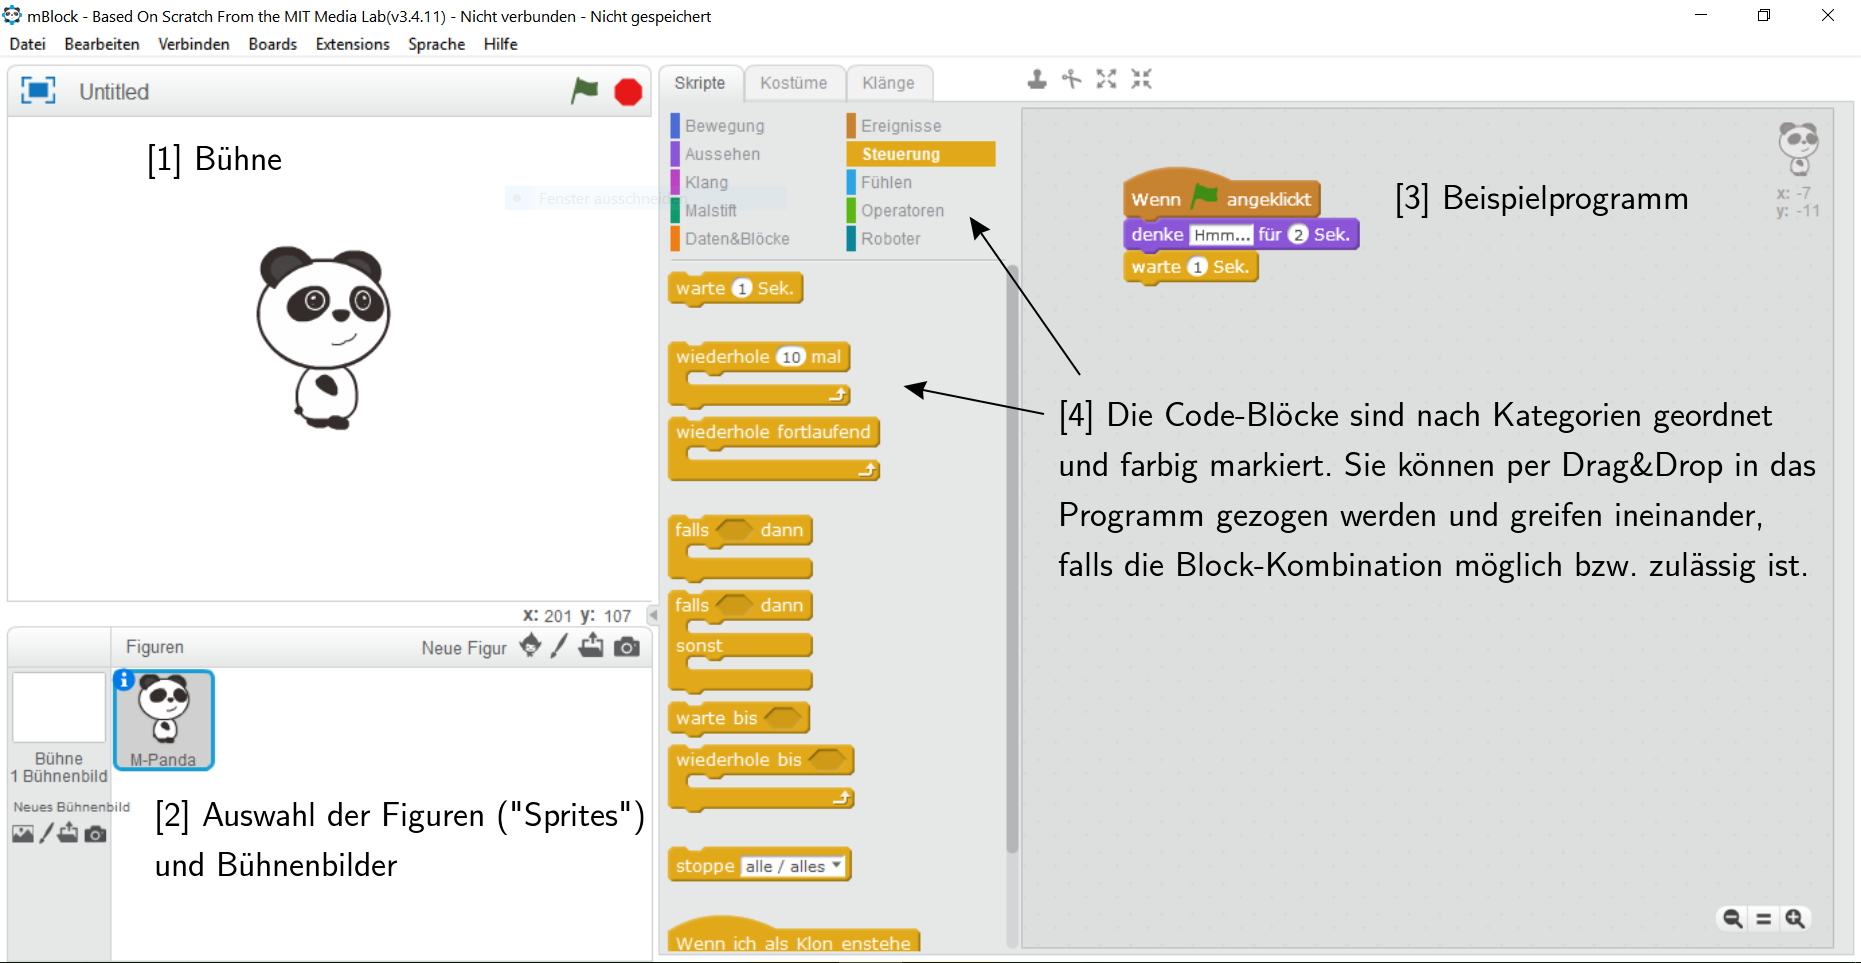
\includegraphics[width=1.2\textwidth]{pics/mblock-uebersicht.PNG}
	\caption{Übersicht über die Programmierumgebung \emph{mBlock}.}
	\label{abb:mblock-uebersicht}
	\end{adjustwidth*}
\end{figure}

	
Für die ersten Programmiererfahrungen machen wir noch nichts mit dem Arduino, sondern kümmern uns nur um die in mBlock eingebaute Bühne.

\marginpar{%
	\textattachfile[description={Folie zu Kap. \thechapter, Auftrag Pandalauf}]{./Auftraege/kap1-auftrag-pandalauf.pdf}{%
	\footnotesize%
	\folie Folie%
	}%
	%\href{run:./Auftraege/kap1-auftrag-pandalauf.pdf}{Folie}\\%
	\footnotesize
	\\öffnen%
}
\begin{ziel}
	\textbf{Ziel:} Der Panda soll auf der Bühne folgendes machen, nachdem auf die grüne Fahne ($\rightarrow$ Ereignisse) geklickt wurde:
	\begin{itemize}[itemsep=0ex]
		\item Der Panda läuft von links nach rechts. ($\rightarrow$ Bewegung)
		\item Der Panda sagt für 1 Sekunde \enquote{Hallo!}. ($\rightarrow$ Aussehen)
		\item Der Panda läuft von rechts nach links.
		\item Der Panda wartet eine Sekunde (und macht dabei nichts).
		\item Der ganze Vorgang wiederholt sich fortlaufend.
	\end{itemize}
\end{ziel}

\emph{Für Schnelle und Kreative:} Erweitere dein Programm, indem du eine andere Bühne oder ein anderes Kostüm auswählst. Spiele mit den Befehlen herum, um dein Programm individuell anzupassen.

\begin{zsfg}{{Programm, Befehl und Argument}}
	\begin{wrapfigure}{r}{0.3\textwidth}
	   \centering
	   
\includegraphics[width=0.3\textwidth]{pics/Befehl-Bsp.png}
	   \caption{Befehl mit Textargument und Zahlargument.}
	   \label{abb:befehlbsp}
	\end{wrapfigure}
	Ein Programm besteht aus einer Folge von Anweisungen oder Befehlen. Man spricht auch von Algorithmen: Ein Algorithmus ist eine eindeutige Handlungsvorschrift zur Lösung eines Problems, die aus endlich vielen Anweisungen besteht (s. \href{https://de.wikipedia.org/wiki/Algorithmus}{Wikipedia}).
	
	Ein Befehl \emph{kann} ein oder mehrere \emph{Argumente} haben, die wiederum einen unterschiedlichen Typ haben können (z.\,B. Text oder (ganze) Zahl).
\end{zsfg}

\begin{aufgabe}
	\textit{Gehübungen}\smallbreak
	Beschreibe jeweils, was der Panda macht, wenn das abgebildete Programm läuft. Streiche, wenn möglich, alle Befehle, die man nicht benötigt.
\end{aufgabe}
\begin{figure}[H]
	\centering
	\subfloat[]{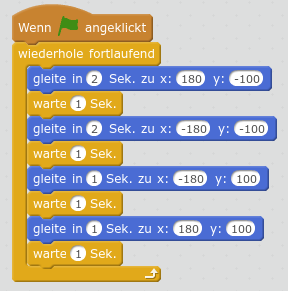
\includegraphics[width=0.37\textwidth]{pics/panda-rechtecklauf.png}}
	\hspace{0.5cm}
	\subfloat[]{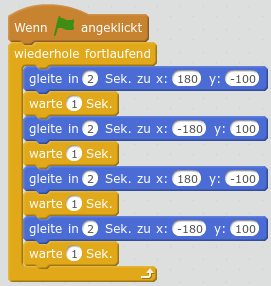
\includegraphics[width=0.35\textwidth]{pics/panda-diagonalenlauf.png}}
	\label{abb:uebungsbsp_befehle}
\end{figure}

\chapter{Einführung in die Welt des Arduino: Digitale Ausgänge und Eingänge}

Der Arduino ist ein Mikrocontroller, der vom italienischen Professor Massimo Banzi entwickelt wurde, damit seine Studenten im Bereich \emph{Design} eine einfach zugängliche Möglichkeit fanden, Elektronik für künstlerische Projekte zu nutzen. Die vorgenommenen Vereinfachungen in der Handhabung von Mikrocontrollern gefielen jedoch nicht nur den Studenten von Massimo Banzi, sondern auch zahlreichen Studenten anderer Fachrichtungen, Schülern, Hobby-Elektronikern und sogar Fachleuten in der Industrie, sodass der Arduino rasch eine weltweite Verbreitung fand.

\bigskip
In diesem Kapitel lernst du\dots
\begin{itemize}
	\item \dots wie der Arduino aufgebaut ist,
	\item \dots wie man den Arduino mit dem PC verbindet und mit mBlock programmiert,
	\item \dots die digitalen Pins als Ausgänge zu benutzen, um eine LED zu steuern,
	\item \dots Schaltungen auf dem Steckbrett aufzubauen,
	\item \dots Widerstand, Spannung und Stromstärke im Stromkreis zu berechnen,
	\item \dots Widerstandsringe abzulesen, um die Größe des Widerstands zu bestimmen,
	\item \dots eine RGB-LED und eine 7-Segmentanzeige zu steuern,
	\item \dots das elektrische Potential an einem digitalen Pin einzulesen und \dots
	\item \dots mit Hilfe des elektrischen Potentials den Zustand eines Tasters abzufragen.
\end{itemize}

\begin{projektueberblick}
	\item Ampel \dotfill \pageref{proj:ampel}
	\item Augentestgerät \dotfill\pageref{proj:augentest}
	\item Farbenspektakel mit RGB-LED \dotfill\pageref{proj:rgbled1}
	\item Raketencountdown \dotfill\pageref{proj:raketencountdown}
	\item Fußgängerampel \dotfill\pageref{proj:fussampel}
	\item Juke-Box \dotfill\pageref{proj:jukebox}
\end{projektueberblick}

\section{Der Aufbau des Arduino UNO}
Mit der Zeit entwickelten sich zahlreiche andere Modelle des Arduino, die kleiner oder größer waren, über mehr oder weniger Anschlüsse verfügten, schneller oder langsamer waren usw. Das Standardmodell ist heute der Arduino Uno, den auch wir verwenden.

\begin{figure}[h]
	\centering
	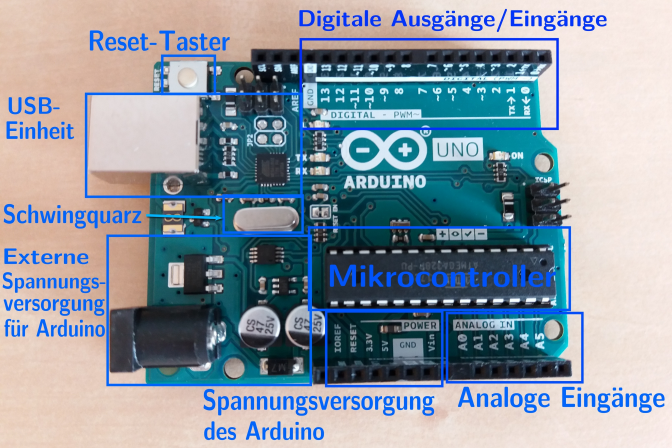
\includegraphics[width=0.8\textwidth]{pics/arduino-beschriftet.png}
	\caption{Die wichtigsten Komponenten eines Arduino Uno.}
	\label{abb:arduino-beschriftet}
\end{figure}

Abbildung \ref{abb:arduino-beschriftet} zeigt die wichtigsten Komponenten des Arduino Uno. Eine genauere Beschreibung dieser Funktionseinheiten und ihrer spezifischen Eigenschaften findet sich in Anhang \ref{sec:ueberblick}. Wichtig sind an dieser Stelle vor allem folgende Punkte:
\begin{itemize}
	\item Über den USB-Anschluss und das mitgelieferte Kabel lässt sich der Arduino mit dem PC verbinden und programmieren.
	\item Das Programm läuft nach dem Übertragen auf dem eigentlichen Mikrocontroller, dem langen schwarzen Ding in der Mitte. Der ganze Rest auf dieser kleinen Platine dient der einfacheren Handhabung des Mikrocontrollers.
	\item An den Seiten befinden sich die Pin-Leisten, an die sich zum Beispiel LEDs anschließen lassen. Die Pins sind durchnummeriert, sodass sie im Programm angesprochen werden können. \emph{GND} steht für \enquote{Ground} oder den Minus-Kontakt. \emph{5V} steht für den Plus-Kontakt und gibt an, dass dort stets eine Spannung von 5V anliegt, wenn der Arduino über USB oder Batterie mit Strom versorgt wird. Die durchnummerierten Digitalpins können durch das Programm ebenfalls auf 5V gesetzt werden (\texttt{HIGH}), aber auch auf 0V, sodass kein Strom fließt (\texttt{LOW}).
\end{itemize}
\vfill

\section{Vorbereitung von \emph{mBlock}}

\begin{figure}[H]
	\begin{adjustwidth*}{-1.5cm}{-1.5cm}
		\centering
		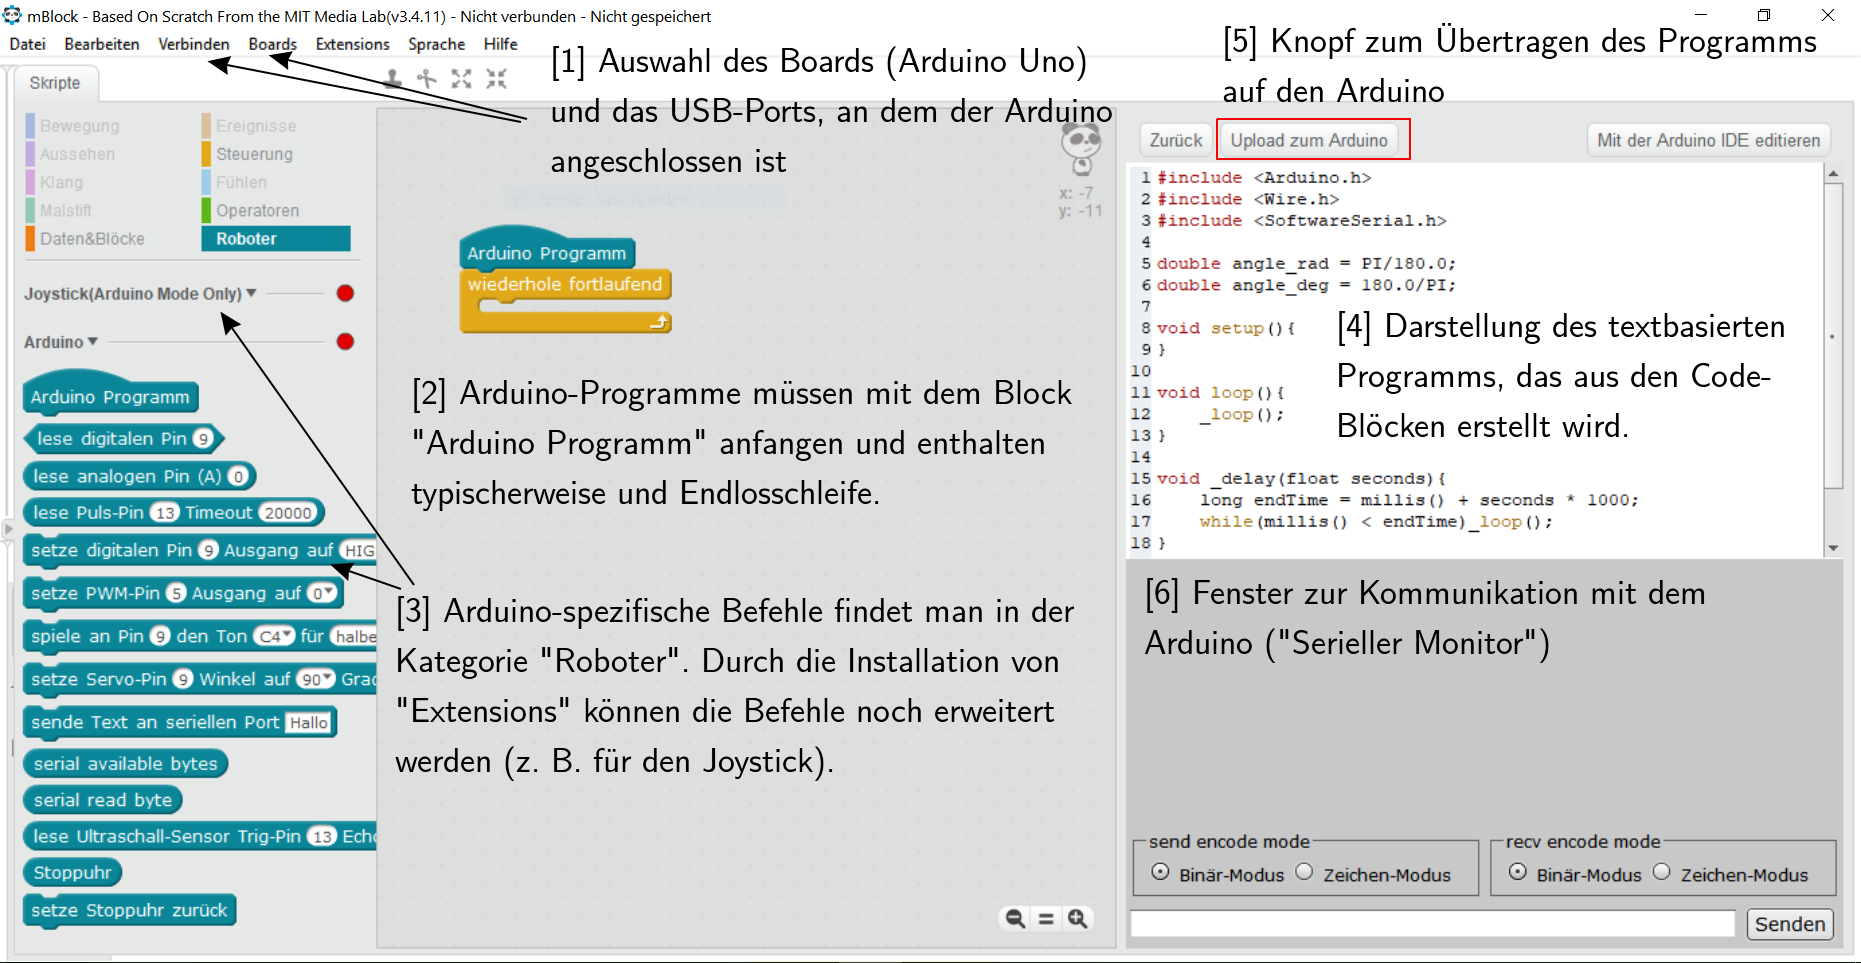
\includegraphics[width=1.2\textwidth]{pics/mblock-arduinomodus.PNG}
		\caption{Übersicht über die Programmierumgebung \emph{mBlock} im Arduino-Modus.}
		\label{abb:mblock-arduinomodus}
	\end{adjustwidth*}
\end{figure}

Die Programmierumgebung \emph{mBlock} wurde im Wesentlichen dafür erstellt, dass man die firmeneigenen Roboter namens \emph{mBot} programmieren kann. Diese basieren auf einem Arduino, der die angeschlossenen Motoren und Sensoren steuert und per \emph{mBlock} programmiert wird. Gleichzeitig ermöglicht es \emph{mBlock} auch, den Arduino als eigenständigen Mikrocontroller zu programmieren. Dies ist der Modus, den wir benutzen werden. Man erreicht diesen Arduino-Modus unter \button{Bearbeiten} $\rightarrow$ \button{Arduino-Modus}. 

Als erstes muss der USB-Port ausgewählt werden, an dem der Arduino angeschlossen ist (unter \button{Verbinden}) und danach muss der Arduino Uno als Board ausgewählt werden (unter \button{Boards}). Damit sind alle Einstellungen vorgenommen, um den Arduino Uno mit mBlock programmieren zu können.

\newpage
\section{Digitale Ausgänge steuern}

\begin{ziel}
	\textbf{Ziel:} Es soll das erste Testprogramm auf den Arduino übertragen werden, mit dem man üblicherweise überprüft, ob der Arduino (oder ein anderer Mikrocontroller) richtig funktioniert. Dazu soll die bordeigene LED zum Blinken gebracht werden:
	\begin{itemize}[itemsep=0ex]
		\item Stelle LED an.
		\item Warte eine Sekunde.
		\item Stelle LED aus.
		\item Warte eine Sekunde.
		\item Wiederhole fortlaufend.
	\end{itemize}
\end{ziel}

\emph{Hinweise:} 
\medskip

\begin{minipage}{0.7\textwidth}
	Arduino-Programme müssen immer mit dem entsprechenden Startblock für ein Arduino-Programm beginnen (siehe Abbildung rechts.)
\end{minipage}
\begin{minipage}[]{0.3\textwidth}
	\centering
	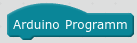
\includegraphics[width=0.75\textwidth]{pics/Arduino_Start_Block.png}
	\label{abb:arduinostartblock}
\end{minipage}


\begin{wrapfigure}{r}{0.4\textwidth}
	\centering
	
\includegraphics[width=0.4\textwidth]{pics/digitalWriteBlock.png}
	\label{abb:digitalwriteblock}
\end{wrapfigure}
Die bordeigene LED ist mit dem (digitalen) Pin Nummer 13 verbunden und kann darüber gesteuert werden. Zur Steuerung von digitalen Pins nutzt man den rechts abgebildeten Block.

Mit dem Knopf \button{Upload zum Arduino} lässt sich das fertige Programm auf den Arduino übertragen. Wenn alles klappt, sollte nun die bordeigene LED blinken.

\begin{aufgabe}
	Wir nutzen in den ersten Kapiteln sehr häufig LEDs, weil sich die Grundlagen mit ihnen einfach erarbeiten lassen, aber auch weil sie eine enorme Bedeutung in der heutigen Welt haben. Notiere dir zur Verdeutlichung eine Woche lang alle Geräte, die dir begegnen oder die dir einfallen, in denen LEDs verbaut sind.
\end{aufgabe}


\newpage
\section{Aufbau von Schaltungen auf der Steckplatine}

In der Regel braucht man für interressante Geräte zusätzliche \emph{Hardware} (Sensoren, Motoren, \dots), die am Arduino angeschlossen wird. Bevor diese fest verlötet werden, nutzt man normalerweise Steckverbindungen bzw. baut die Schaltung auf einem kleinen Steckbrett auf, auf dem man die Verbindungen schnell wieder lösen kann, falls nötig. Steckbretter sind aus dem Physikunterricht bekannt. Abbildung \ref{abb:steckbrett} zeigt, welche Kontakte auf dem Steckbrett miteinander verbunden sind.

\begin{figure}[h]
	\centering
	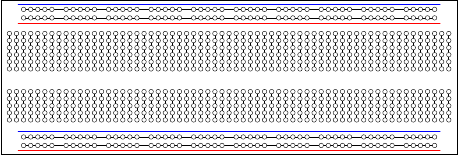
\includegraphics[width=0.8\textwidth]{./Zeichnungen/steckbrett.png}
	\caption{Die Steckverbindungen sind außen in Längsrichtung und innen in Querrichtung miteinander verbunden.}
	\label{abb:steckbrett}
\end{figure}

\begin{ziel}
	\textbf{Ziel:} Eine externe LED an Pin 13 soll zum Leuchten gebracht werden. Diese kann genutzt werden, um das Blinken einer Alarmanlagen-LED zu simulieren.
\end{ziel}

\emph{Hinweise:} 

Es kann das Programm aus dem vorherigen Abschnitt wieder verwendet werden. Allerdings gibt es ein Problem: Wenn der digitale Pin auf \texttt{HIGH} gesetzt wird, bedeutet das, dass er eine Spannung von 5V gegenüber GND ausgibt. Die LED verträgt jedoch nur (je nach Farbe) gut 2 V. Daher ist die LED mit einem Vorwiderstand von $\SI{330}{\SIUnitSymbolOhm}$ verbunden.

Die LED ist ein sogenanntes gepoltes Bauteil. Das heißt, dass einer der Kontaktstifte der LED an den Plus-Kontakt angeschlossen werden \emph{muss} und der andere an den Minus-Kontakt angeschlossen werden \emph{muss}.

%\bigskip
%\textbf{Projekt 1: Ampel}
\begin{projekt}[Ampel]\label{proj:ampel}
	Baue und programmiere eine Ampelschaltung!
	
	\emph{Für Schnelle:} Erweitere die Ampel um einen Nachtmodus.
\end{projekt}

%\bigskip
%\textbf{Projekt 2: Augentestgerät}

\begin{projekt}[Augentestgerät]\label{proj:augentest}
	Moderne Fernseher nutzen meist eine Bildwiederholungsrate von 144 Hertz; das bedeutet, es werden 144 Bilder pro Sekunde eingespielt. Finde mithilfe des Blink-Programms heraus, ab welchem Blinkintervall du kein Flackern mehr wahrnimmst und berechne, wie viele \enquote{Bilder} pro Sekunde sich daraus ergeben. Vergleiche diesen Wert mit der Bildwiederholungsrate im Fernsehen.
	
	{\scriptsize Idee: Frick, Fritsch und Trick (2015): \emph{Einführung in Mikrocontroller - Der Arduino als Steuerzentrale}, Bad Saulgau}
\end{projekt}


\newpage

\section{Widerstand, Spannung und elektrische Stromstärke berechnen}

\begin{wrapfigure}{r}{0.2\textwidth}
	\centering
	\vspace{-\baselineskip}
	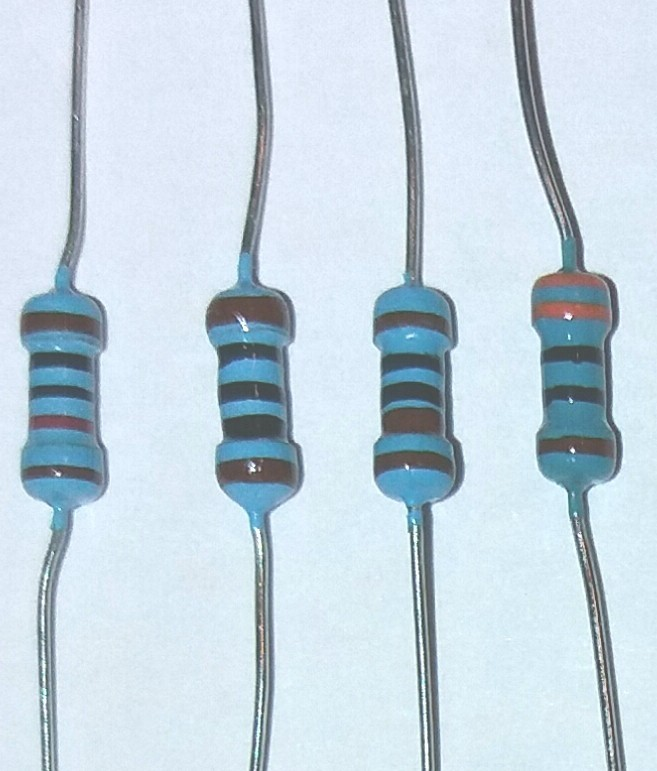
\includegraphics[width=0.18\textwidth,angle=90]{pics/Widerstaende.jpg}
	\vspace{-3\baselineskip}
	\label{abb:widerstaende}
\end{wrapfigure}
Im vorherigen Abschnitt war die Größe des Vorwiderstands mit $\SI{330}{\SIUnitSymbolOhm}$ vorgegeben. 
In unserem Bausatz finden sich jedoch viele weitere Widerstände, die teilweise größer und teilweise kleiner sind.

\textbf{Vorüberlegung:} Wird die LED heller oder dunkler leuchten, wenn man den Vorwiderstand vergrößert? Begründe deine Vermutung.

\begin{figure}[H]
	\centering
	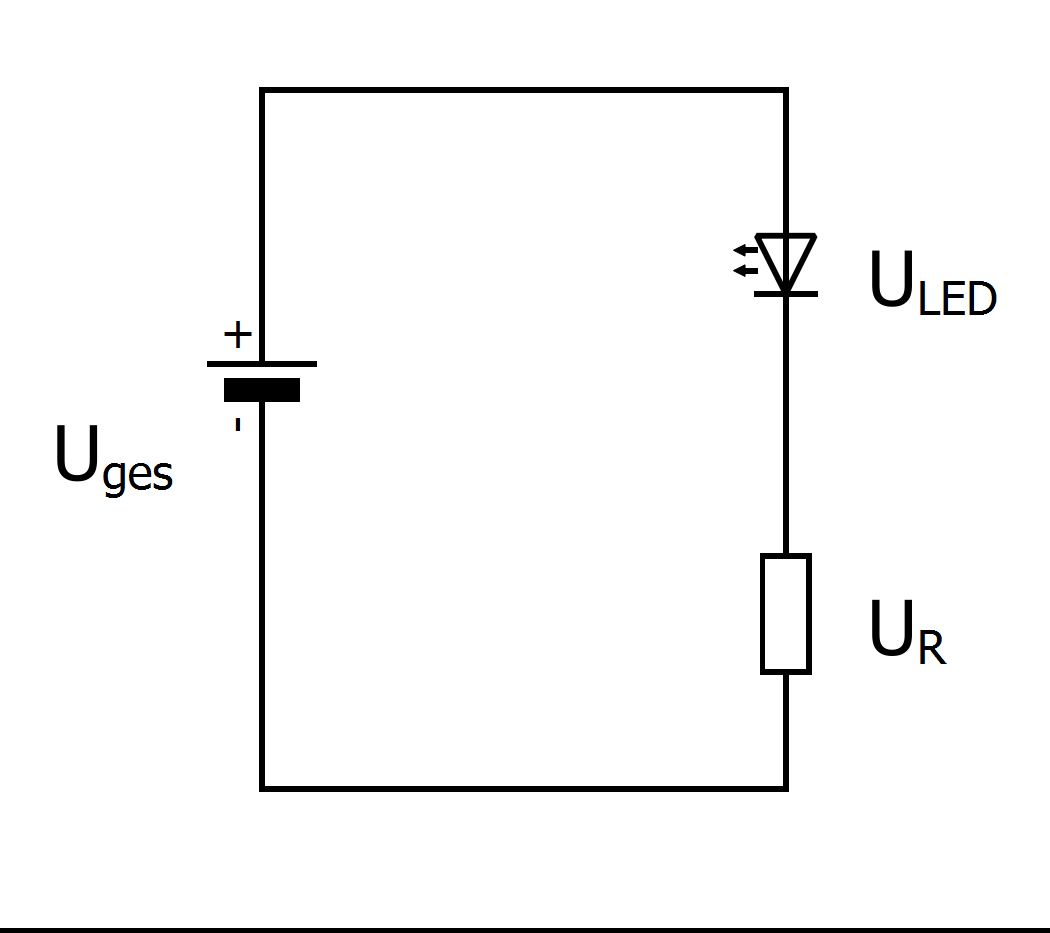
\includegraphics[width=0.35\textwidth]{./Zeichnungen/ReiheLEDWiderstand.png}
	\caption{Reihenschaltung von LED und Vorwiderstand an einer Spannungsquelle.}
	\label{abb:reiheledwiderstand}
\end{figure}
% Vorüberlegungen zur gleichzeitigen Wiederholung der Gesetze für die Reihenschaltung:
% Der Strom durch den Widerstand wird kleiner, wenn der Widerstand größer wird. Da die Stromstärke überall gleich groß ist, wird auch die Stromstärke in der LED kleiner.
% Die LED leuchtet, weil sie elektrische Energie in Lichtenergie umwandelt. Ein Maß für die elektrische Energie der Teilchen ist die Spannung. Wenn der Widerstand größer wird, wird auch die Spannung, die dort abfällt, größer (die Teilchen brauchen mehr Energie, um hindurch zu kommen). Daher wird die Spannung an der LED kleiner, denn die Gesamtspannung von 5V bleibt gleich und beide Spannungen addieren sich zur Gesamtspannung.
% Die Widerstände der Bauteile addieren sich ebenfalls zum Gesamtwiderstand.

Nach den Vorüberlegungen ist klar, dass ein größerer Widerstand für die LED kein Problem darstellt. Aber wie sieht es mit einem kleineren Widerstand aus? Der Widerstand muss schließlich in jedem Fall verhindern, dass die LED stärker belastet wird als sie aushält\dots

\begin{ziel}
	\textbf{Frage:} Wie groß muss der Vorwiderstand einer LED mindestens sein, damit sie nicht durchbrennt?
\end{ziel}

\emph{Hinweise:}
\begin{itemize}[itemsep=0mm,parsep=0mm]
	\item Wenn ein Digitalpin auf \texttt{HIGH} gesetzt wird, dann gibt er eine Spannung von 5V gegenüber GND aus.
	\item Durch eine LED darf höchstens ein Strom von $\SI{20}{\milli\ampere}$ fließen.
	\item Je nach Farbe halten LEDs eine andere maximale Spannung aus:
	
	\begin{tabular}{l|l|l|l}
		Farbe & rot & gelb/grün & blau/weiß \\ \hline
		$U_{LED}$ & 1,6\,V - 2,2\,V & 1,9\,V - 2,5\,V & 2,7\,V - 3,5\,V \\
	\end{tabular}
\end{itemize}

\begin{zsfg}{{Widerstand, Spannung und Stromstärke}}
	\begin{wrapfigure}{r}{0.15\textwidth}
		\vspace{-\baselineskip}
		\begin{tikzpicture}
			\draw [black, thick] (0,0) -- (0.8,1.5) -- (1.6,0) -- (0,0);
			\node at (0.8,0.9) {\color{black}$U$};
			\draw [black, thick] (0.5,0.6) -- (1.1,0.6);
			\node at (0.5,0.2) {\color{black}$R$};
			\node at (1.1,0.2) {\color{black}$I$};
		\end{tikzpicture}
	\end{wrapfigure}
	Der Widerstand $R$ ist definiert als das Verhältnis von Spannung $U$ zu Stromstärke $I$:
	\begin{equation*}
		R=\frac{U}{I}.
	\end{equation*}
	
	Ein Widerstand heißt \emph{ohmscher Widerstand}, wenn das Verhältnis $\frac{U}{I}$ stets gleich groß ist (also wenn $R$ unabhängig von Stromstärke und Spannung konstant ist).
\end{zsfg}
\begin{tcolorbox}[equal height group=A,enhanced, colback=CadetBlue!70!green, coltext=black, colframe=DarkCyan!70!DarkGreen, width=0.48\textwidth, before=, after=\hfill, adjusted title={Elektrische Stromstärke und Spannung in der Reihenschaltung}, colbacktitle=CadetBlue!70!green, coltitle=black, fonttitle=\bfseries]
	\begin{figure}[H]
		\centering
		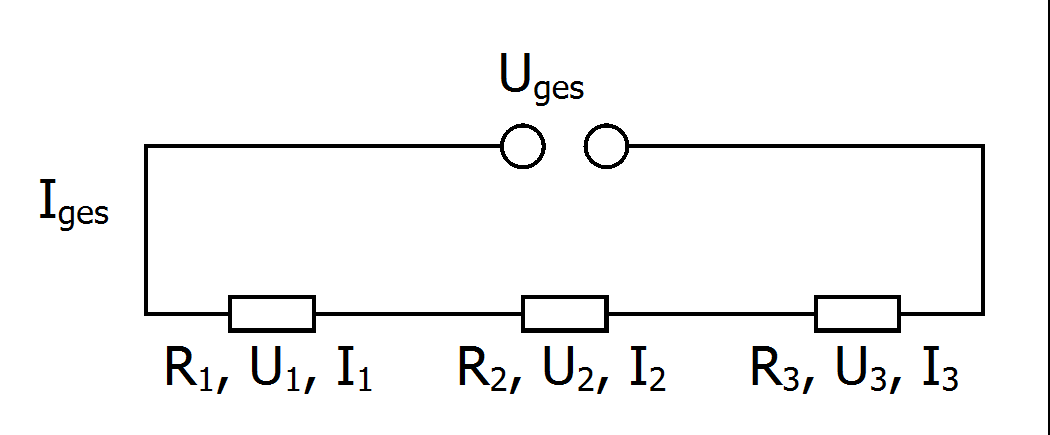
\includegraphics[width=\textwidth]{./Zeichnungen/reihenschaltung.png}
	\end{figure}
	\begin{itemize}[parsep=0ex,itemsep=0ex,leftmargin=*]
		\item In einer Reihenschaltung ist die Stromstärke an jeder Stelle gleich groß:
		\begin{equation*}
			I_{ges}=I_1=I_2= I_3=\dots
		\end{equation*}
		\item In einer Reihenschaltung teilt sich die Gesamtspannung auf die einzelnen Bauteile auf:
		\begin{equation*}
			U_{ges}=U_1 + U_2 + U_3+\dots
		\end{equation*}
		\item In einer Reihenschaltung addieren sich die Einzelwiderstände zum Gesamtwiderstand:
		\begin{equation*}
			R_{ges}=R_1+R_2+R_3+\dots
		\end{equation*}
	\end{itemize}
\end{tcolorbox}
\begin{tcolorbox}[equal height group=A,enhanced, colback=CadetBlue!70!green, coltext=black, colframe=DarkCyan!70!DarkGreen, width=0.48\textwidth, before=, after=\hfill, adjusted title={Elektrische Stromstärke und Spannung in der Parallelschaltung}, colbacktitle=CadetBlue!70!green, coltitle=black,fonttitle=\bfseries]
	\begin{figure}[H]
		\centering
		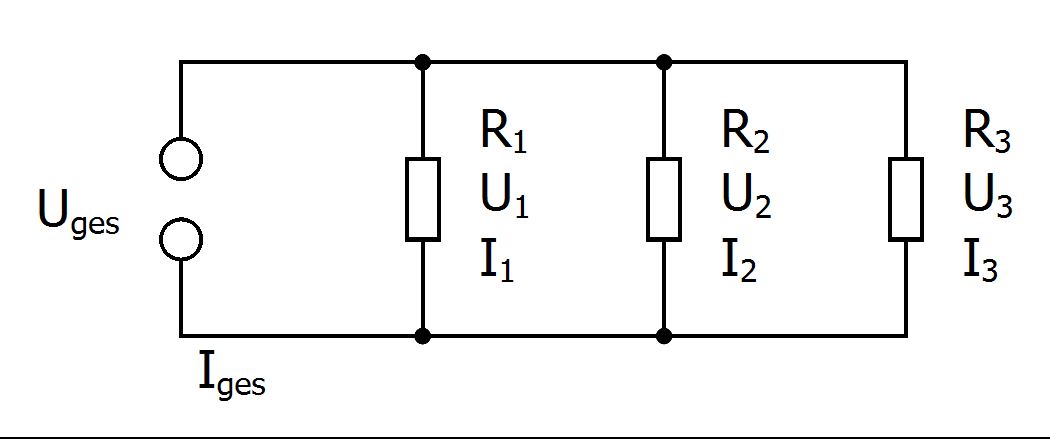
\includegraphics[width=\textwidth]{./Zeichnungen/parallelschaltung.png}
	\end{figure}
	\begin{itemize}[parsep=0ex,itemsep=0ex,leftmargin=*]
		\item In einer Parallelschaltung teilt sich die Gesamtstromstärke auf die einzelnen Zweige auf:
		\begin{equation*}
			I_{ges}=I_1+I_2+ I_3+\dots
		\end{equation*}
		\item In einer Parallelschaltung ist die Spannung in jedem Zweig gleich groß:
		\begin{equation*}
			U_{ges}=U_1=U_2=U_3=\dots
		\end{equation*}
		\item In einer Parallelschaltung ist der Kehrwert des Gesamtwiderstands gleich der Summe der Kehrwerte der einzelnen Widerstände:
		\begin{equation*}
			\frac{1}{R_{ges}} = \frac{1}{R_1} + \frac{1}{R_2} + \frac{1}{R_3} + \dots
		\end{equation*}
	\end{itemize}
\end{tcolorbox}

\begin{aufgabe}
	In unserem Starter Kit ist ein 9V Akku untergebracht. Berechne den mindestens notwendigen Vorwiderstand, wenn eine
	rote LED an den 9V Block angeschlossen wird.
\end{aufgabe}

\begin{aufgabe}
	\smallbreak
	\textbf{a)} An dem 9V Block sollen drei rote LEDs in Reihe geschaltet betrieben werden. Zeichne jeweils einen Schaltplan und berechne den passenden Vorwiderstand.
	
	\textbf{b)} An dem 9V Block sollen drei rote LEDs parallel geschaltet betrieben werden. Zeichne jeweils einen Schaltplan und berechne den passenden Vorwiderstand.
\end{aufgabe}
\vfill

\newpage
\begin{projekt}[Farbenspektakel mit RGB-LED]\label{proj:rgbled1}
	
	\smallskip
	\begin{minipage}{0.45\textwidth}
		Mit einer RGB-LED können die verschiedensten Farben erzeugt werden, die zum Beispiel in Smartphones als Status-LED genutzt werden. RGB steht für Rot, Grün und Blau. In einer RGB-LED sind also drei LEDs gleichzeitig verbaut, die sich in unserem Fall eine gemeinsame Anode (Kontakt mit GND) teilen. Die Anode gehört zum längsten Beinchen.
	\end{minipage}
	\hfill
	\begin{minipage}{0.5\textwidth}
		\begin{figure}[H]
			\hfill
			\begin{minipage}{0.48\textwidth}
				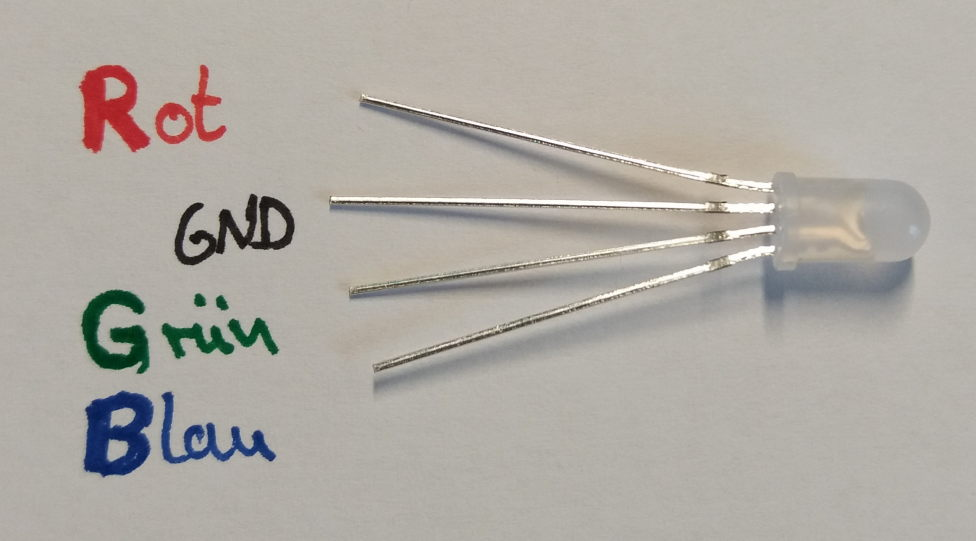
\includegraphics[width=\textwidth]{pics/rgb-led.jpg}
				\caption{RGB-LED}
			\end{minipage}
			\hfill
			\begin{minipage}{0.48\textwidth}
				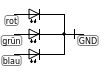
\includegraphics[width=\textwidth]{pics/rgb-led-schaltplan.png}
				\caption{Verschaltung der RGB-LED.}
			\end{minipage}
			\hfill
			\label{abb:rgb-led}
		\end{figure}
	\end{minipage}
	\bigskip
	
	\begin{wrapfigure}{r}{0.25\textwidth}
		\centering
		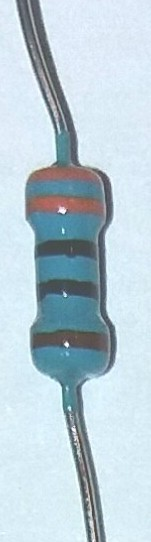
\includegraphics[angle=90,width=0.2\textwidth]{pics/330ohm.jpg}
	\end{wrapfigure}
	Schließe die RGB-LED an den Arduino an. \emph{Achte darauf, dass zwischen den Plus-Kontakten der LEDs und den digitalen Pins ein Widerstand von von $\SI{330}{\ohm}$ geschaltet ist.} Der Widerstand lässt sich an der Reihenfolge der Ringe erkennen: Orange - Orange - Schwarz - Schwarz - Braun.
	
	\medbreak
	\textbf{a)} Experimentiere mit den verschiedenen Farben. Notiere dir alle möglichen Farbtöne und wie diese zusammengesetzt sind.
		
	\medskip
	\textbf{b)} \emph{Zur Reflexion der Berechnung des Vorwiderstands:} Begründe, warum der unten berechnete Vorwiderstand zu niedrig ist. Erkläre, wie man stattdessen vorgehen müsste und gib den korrekten Wert für einen möglichen gemeinsamen Vorwiderstand an.
\end{projekt}
\marginpar{%
	\parbox{1.5cm}{%
		\footnotesize%
		Wie man weitere Farben erzeugt, erfährst du in \ref{proj:rgbled2}.
	}
}

\vspace{2\baselineskip}
\begin{tcolorbox}[sharp corners]
	\begin{wrapfigure}{r}{0.4\textwidth}
		\centering
		\vspace{-\baselineskip}
		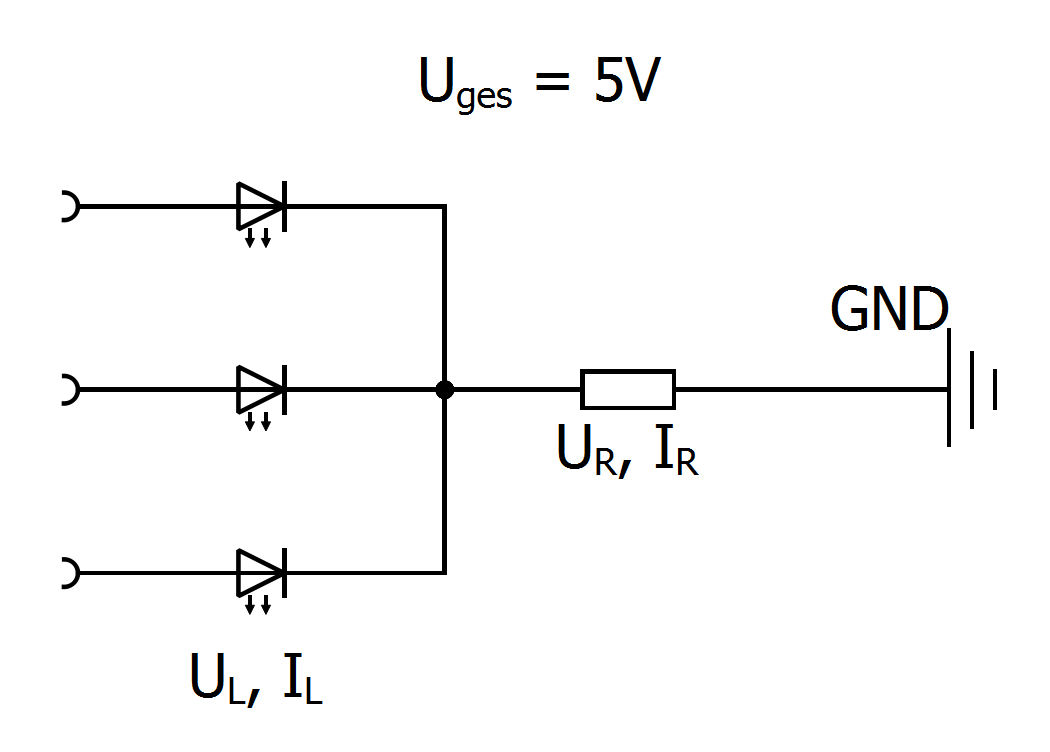
\includegraphics[width=0.4\textwidth]{./Zeichnungen/schaltplan-rgb-led-berechnung.png}
	\end{wrapfigure}
	$I_L = \SI{20}{\milli\ampere} = \SI{0,02}{\ampere} \quad \Longrightarrow \quad I_R = \SI{0,06}{\milli\ampere}$
	
	$U_L = \SI{2,2}{\volt}$ \quad (max. Spannung, die rote LEDs aushalten)
	
	$U_R = \SI{5}{\volt} - \SI{2,2}{\volt} = \SI{2,8}{\volt}$
	
	\begin{equation*}
		R = \frac{U_R}{I_R} = \frac{\SI{2,8}{\volt}}{\SI{0,06}{\ampere}} \approx \SI{46,67}{\ohm}
	\end{equation*}
	
	\bigskip
	Der Vorwiderstand sollte eine Größe von mindestens $\SI{50}{\ohm}$ haben.
\end{tcolorbox}

%Das Problem ist, dass auch nur eine LED angeschaltet sein kann und dann darf der Gesamtwiderstand nur 0,02 A durchlassen, muss also größer sein.

\newpage
\section{Widerstandsringe ablesen}

Leider sind die Widerstände zu klein, um ihren Wert darauf gut lesbar zu drucken. Daher werden die Widerstände mit Ringen versehen, aus deren Farbe sich die Größe des Widerstands ablesen lässt. Um den für die 7-Segment-Anzeige passenden Widerstand aus dem Bausatz auszuwählen, müssen wir diesen Farbcode lesen können.

Bei den blauen Kohleschichtwiderständen, die wir verwenden, gibt es fünf Ringe und jede Ringfarbe steht für eine Zahl. Die ersten drei Ringe bilden die ersten drei Ziffern des Widerstandswertes ab. Die darauf folgende Ringfarbe steht für die Zehnerpotenz, die mit den drei Ziffern multipliziert werden muss. Dies dient dazu, auch größere Widerstandswerte codieren zu können. Der letzte Ring wiederum soll einen etwas größeren Abstand haben und steht für die Fehlertoleranz des Widerstandswertes. In der Praxis lässt sich allerdings nicht immer gut erkennen, welcher Ring der letzte und welcher der erste ist\dots

\begin{figure}[H]
	\centering
	\begin{tikzpicture}[scale=0.35]
	\shade [top color=lightgray, bottom color=gray] (-5,0.8) rectangle (10,1.2);
	\shade [top color=LightSkyBlue, bottom color=NavyBlue] (0,0) -- (5,0) arc [start angle=-135, end angle=135, radius=1.414] -- (0,2) arc [start angle=45, end angle=315, radius=1.414];
	\draw [fill=orange] (0,0) rectangle ++(0.5,2) ++(-0.25,-1) -- ++(0,-1.25) [anchor =north] node {\Large 3};
	\draw [fill=green] (1,0) rectangle ++(0.5,2) ++(-0.25,-1) -- ++(0,-1.25) [anchor =north] node {\Large 5};
	\draw [fill=black] (2,0) rectangle ++(0.5,2) ++(-0.25,-1) -- ++(0,-1.25) [anchor =north] node {\Large 0};
	\draw [fill=black] (3,0) rectangle ++(0.5,2) ++(-0.25,-1) -- ++(0.5,-1.25) [anchor =north] node {\Large $\times 1$};
	\draw [fill=brown] (4.5,0) rectangle ++(0.5,2) ++(-0.25,-1) -- ++(1.5,-1.8) [anchor =north] node {\Large $\pm1\%$};
	\end{tikzpicture}
\end{figure}
Ein Beispiel: Die Ringfarben lauten orange - grün - schwarz - schwarz - braun. Anhand der folgenden Tabelle lässt sich daraus der Wert konstruieren: $3 - 5 - 0 - \cdot 1 (=10^0) - \pm 1\% $, kurz: $\SI{350}{\SIUnitSymbolOhm}\pm\SI{3,5}{\SIUnitSymbolOhm}$.

\begin{table}[H]
   \centering
   %\rowcolors{1}{lightgray}{white}
   \begin{minipage}[c]{\textwidth}
      \begin{tabu} to \textwidth {X[L,2]X[C]X[C]X[C]X[C,3]X[C,2]}
         \toprule
         \textbf{Ringfarbe} & \textbf{1. Ring} & \textbf{2. Ring} & \textbf{3. Ring} & \textbf{4. Ring (Multiplikator)} & \textbf{5. Ring (Toleranz)} \\
         \midrule
         \textcolor{black}{\rule{1cm}{0.4cm}} Schwarz & 0 & 0  & 0 & $\times 1$ / $\times 10^0$ & - \\
         \textcolor{brown}{\rule{1cm}{0.4cm}} Braun   & 1 & 1 & 1& $\times10$ / $\times 10^1$ & 1\% \\
         \textcolor{red}{\rule{1cm}{0.4cm}} Rot  & 2 & 2 & 2& $\times100$ / $\times 10^2$ & 2\% \\
         \textcolor{orange}{\rule{1cm}{0.4cm}} Orange & 3 & 3 & 3& $\times 1000$ / $\times 10^3$ & - \\
         \textcolor{yellow}{\rule{1cm}{0.4cm}} Gelb & 4 & 4 & 4& $\times 10.000$ / $\times 10^4$ & - \\
         \textcolor{green}{\rule{1cm}{0.4cm}} Grün  & 5 & 5 & 5& $\times 100.000$ / $\times 10^5$ & - \\
         \textcolor{blue}{\rule{1cm}{0.4cm}} Blau  & 6 & 6 & 6& $\times 1.000.000$ / $\times 10^6$ & - \\
         \textcolor{violet}{\rule{1cm}{0.4cm}} Lila & 7 & 7 & 7& - & - \\
         \textcolor{gray}{\rule{1cm}{0.4cm}} Grau   & 8 & 8 & 8& - & - \\
         \tikz \draw (0,0) rectangle (1,0.4); Weiß & 9 & 9 & 9& - & - \\
         \textcolor{Gold}{\rule{1cm}{0.4cm}} Gold & - & - & -& $\times 0.1$ / $\times 10^{-1}$ & 5\% \\
         \textcolor{lightgray}{\rule{1cm}{0.4cm}} Silber & - & - & -& $\times 0.01$ / $\times 10^{-2}$ & 10\% \\
         \bottomrule
      \end{tabu}
   \end{minipage}
   \caption{Tabelle zur Codierung der Widerstandswerte durch Farbringe.}
   \label{tab:farbcodierung}
\end{table}

\begin{aufgabe}
	Gib die Farbcodierung für einen Widerstand mit den folgenden Werten an:
	\begin{multicols}{2}
		\begin{enumerate}[label=\alph*),itemsep=0ex]
			\item $\SI{435}{\SIUnitSymbolOhm} (\pm 2\%)$,
			\item $\SI{570}{\kilo\SIUnitSymbolOhm} (\pm 5\%)$.
		\end{enumerate}
	\end{multicols}
\end{aufgabe}

\vfill
\newpage
\begin{aufgabe}
	
	\begin{minipage}{0.78\textwidth}
		\textbf{a)} Die rechte Abbildung zeigt die vier wichtigsten Widerstände, mit denen wir zu tun haben werden. Bestimme die jeweilige Größe der Widerstände.
		
		\textbf{b)} Thorsten hat die Ringe eines Widerstands abgelesen: Silber - rot - lila - lila - grün. Bestimme die Größe des Widerstands.
	\end{minipage}
	\hfill
	\begin{minipage}{0.2\textwidth}
		\begin{figure}[H]
			\centering
	%		\vspace{-\baselineskip}
			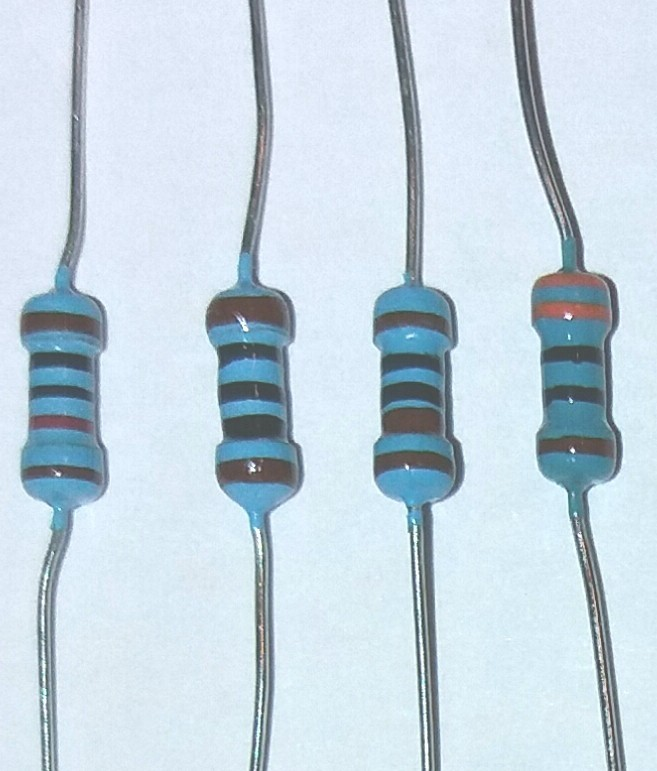
\includegraphics[width=0.8\textwidth,angle=90]{pics/Widerstaende.jpg}
			\label{abb:widerstaende2}
		\end{figure}
	\end{minipage}
	
	\medskip
	\emph{Zur Kontrolle:} \url{https://www.elektronik-kompendium.de/sites/bau/1109051.htm}
\end{aufgabe}


\subsection{Einfache Verwendung einer 7-Segment-Anzeige}

\begin{minipage}{0.58\textwidth}
	Unsere 7-Segment-Anzeige besteht aus sieben roten LEDs, die so angeordnet sind, dass sich mit ihnen eine Zahl darstellen lässt. Zusätzlich gibt es  zur leichteren Unterscheidung von 6 und 9 eine LED für den Punkt. \emph{Jede LED lässt sich einzeln über einen der Pins ansteuern, wobei sich alle LEDs einen gemeinsamen GND-Anschluss teilen.} Der zweite GND-Anschluss soll hier nicht genutzt werden, um die Schaltung so einfach wie möglich zu halten. Es wäre sehr umständlich, für jede LED einen eigenen Vorwiderstand anzuschließen; praktischer ist es, einen einzigen Vorwiderstand zwischen GND-Anschluss der 7-Segment-Anzeige und GND-Anschluss des Arduino anzubringen.
\end{minipage}
\hfill
\begin{minipage}{0.4\textwidth}
	\begin{figure}[H]
		\hfill
		\begin{minipage}{0.48\textwidth}
			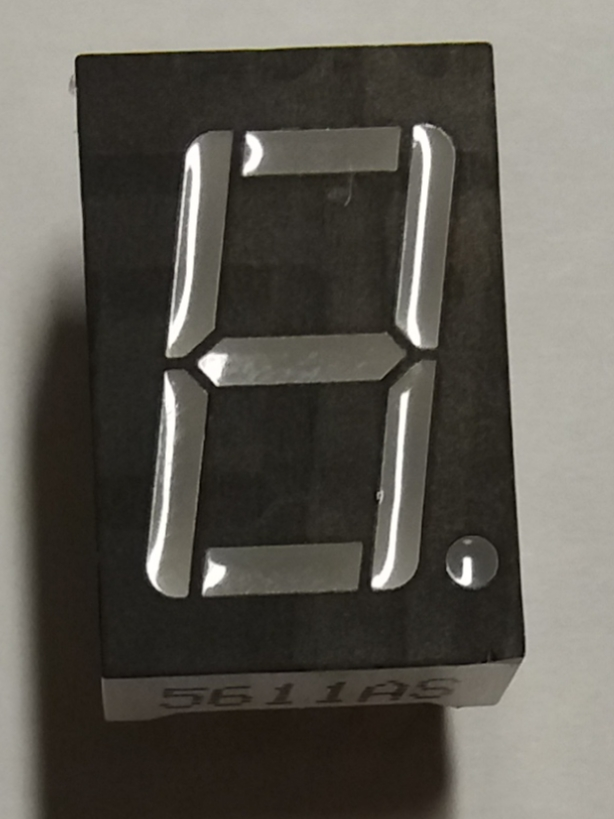
\includegraphics[width=\textwidth]{pics/7segmentanzeige-bild2.jpg}
			\caption{7-Segment-Anzeige}
			\label{abb:7segment-bild}
		\end{minipage}
		\hfill
		\begin{minipage}{0.48\textwidth}
			\begin{tikzpicture}[scale=0.5]
	% Rahmen der Anzeige
	\draw [fill=black] (0,0) rectangle (5.5,7);
	% Segment D
	\draw [fill = white] (1,1) -- ++(0.5,-0.5) -- ++ (1.5,0) -- ++ (0.5,0.5) -- ++ (-0.5,0.5) -- ++ (-1.5,0) -- ++(-0.5,-0.5)  node at ++(1.3,0) (segD) {D}; 
	% Segment G
	\draw [fill = white] (1,3.5) -- ++(0.5,-0.5) -- ++ (1.5,0) -- ++ (0.5,0.5) -- ++ (-0.5,0.5) -- ++ (-1.5,0) -- ++(-0.5,-0.5)  node at ++(1.3,0) (segG) {G};
	% Segment A
	\draw [fill = white] (1,6) -- ++(0.5,-0.5) -- ++ (1.5,0) -- ++ (0.5,0.5) -- ++ (-0.5,0.5) -- ++ (-1.5,0) -- ++(-0.5,-0.5)  node at ++(1.3,0) (segA) {A};
	% Segment E
	\draw [fill = white] (1,1) -- ++ (0.5,0.5) -- ++ (0,1.5) -- ++ (-0.5,0.5) -- ++ (-0.5,-0.5) -- ++ (0,-1.5) -- ++ (0.5,-0.5) node at ++ (0,1.3) (segE) {E};  
	% Segment C
	\draw [fill = white] (3.5,1) -- ++ (0.5,0.5) -- ++ (0,1.5) -- ++ (-0.5,0.5) -- ++ (-0.5,-0.5) -- ++ (0,-1.5) -- ++ (0.5,-0.5) node at ++ (0,1.3) (segC) {C};
	% Segment F
	\draw [fill = white] (1,3.5) -- ++ (0.5,0.5) -- ++ (0,1.5) -- ++ (-0.5,0.5) -- ++ (-0.5,-0.5) -- ++ (0,-1.5) -- ++ (0.5,-0.5) node at ++ (0,1.3) (segF) {F};
	% Segment B
	\draw [fill = white] (3.5,3.5) -- ++ (0.5,0.5) -- ++ (0,1.5) -- ++ (-0.5,0.5) -- ++ (-0.5,-0.5) -- ++ (0,-1.5) -- ++ (0.5,-0.5) node at ++ (0,1.3) (segB) {B};
	% Punkt DP
	\draw [fill = white] (4.5,0.8) circle [radius=0.7cm] node (segDP) {DP};
	% Kontaktstifte
	\foreach \x in {0.5, 1.5, ..., 4.5} {
		\draw [draw=gray, fill=gray] (\x,0) rectangle ++(0.4,-1);
		\draw [draw=gray, fill=gray] (\x,7) rectangle ++(0.4,1);
	}
	% Nummerierung der Kontaktstifte
	\node at (1-0.3,-1.5) [circle, draw, inner sep=1pt] (pin1) {1};
	\node at (2-0.3,-1.5) [circle, draw, inner sep=1pt] (pin2) {2};
	\node at (3-0.3,-1.5) [circle, draw, inner sep=1pt] (pin3) {3};
	\node at (4-0.3,-1.5) [circle, draw, inner sep=1pt] (pin4) {4};
	\node at (5-0.3,-1.5) [circle, draw, inner sep=1pt] (pin5) {5};
	%	\foreach \x in {9,...,6}{
	%		\node at (11-\x-0.3,8.5) [circle, draw, inner sep=1pt] {\x};
	%	}
	\node at (1-0.3,8.5) [circle, draw, inner sep=1pt] (pin10) {\footnotesize 10};
	\node at (11-9-0.3,8.5) [circle, draw, inner sep=1pt] (pin9) {9};
	\node at (11-8-0.3,8.5) [circle, draw, inner sep=1pt] (pin8) {8};
	\node at (11-7-0.3,8.5) [circle, draw, inner sep=1pt] (pin7) {7};
	\node at (11-6-0.3,8.5) [circle, draw, inner sep=1pt] (pin6) {6};
	\node at (2.7,-2.4) {\scriptsize\sffamily GND};
	\node at (2.7,9.3) {\scriptsize\sffamily GND};
	% Verbindungen
	\draw [gray!30!white, thick] (segA) to [out=35,in=270] (pin7); %out= Winkel beim Verlassen, in = Winkel beim Eintreffen
	\draw [gray!30!white, thick] (segB) to [out=60,in=270] (pin6);
	\draw [gray!30!white, thick] (segC) to [out=-90,in=90] (pin4);
	\draw [gray!30!white, thick] (segD) to [out=-120,in=90] (pin2);
	\draw [gray!30!white, thick] (segE) to [out=-90,in=90] (pin1);
	\draw [gray!30!white, thick] (segF) to [out=100,in=270] (pin9);
	\draw [gray!30!white, thick] (segG) to [out=90,in=270] (pin10);
	\draw [gray!30!white, thick] (segDP) to [out=-70,in=90] (pin5);
\end{tikzpicture}
			\caption{Pin-Diagramm der 7-Segment-Anzeige.}
			\label{abb:7segment-pins}
		\end{minipage}
		\hfill
	\end{figure}
\end{minipage}

\begin{aufgabe}
	\begin{enumerate}[label=\alph*), itemsep=0ex,parsep=0mm]
		\item Zeichne einen vereinfachten Schaltplan der 7-Segment-Anzeige, %
		\marginpar{%
			\textattachfile[description={Druckvorlage zu Kap. \thechapter, Schaltplan mit Arduino}]{./Zeichnungen/Schaltplan-Arduino-Vorlage.pdf}{
			\footnotesize%
			\drucker Vorlage%
			}%
			%\href{run:./Zeichnungen/Schaltplan-Arduino-Vorlage.pdf}{Vorlage}% ./ verweist auf das aktuelle Verzeichnis; ../ auf das übergeordnete
			\footnotesize%
			\\öffnen%
		}
		in dem die LEDs einzeln eingezeichnet sind.
		\item Als gemeinsamen Vorwiderstand der acht LEDs (Anzeige \& Punkt) nutzen wir einen $\SI{330}{\ohm}$-Widerstand. Berechne die Gesamtstromstärke und die Stromstärke in jeder LED bei Darstellung einer 1 und einer 8 (jeweils ohne Punkt).
	\end{enumerate}
\end{aufgabe}

\begin{projekt}[Raketencountdown]\label{proj:raketencountdown}
	Suche dir nun einen passenden Widerstand für die 7-Segment-Anzeige heraus und verbinde beide mit dem Arduino. Programmiere dann einen Raketencountdown, der von 9 rückwärts bis 0 zählt.
	
	\emph{Tipp:} Erstelle dir zuerst eine Tabelle, in der du übersichtlich festhälst, welche LEDs für welche Zahl an sein müssen und mit welchen Pins am Arduino diese verbunden sind.
	
	\emph{Für Schnelle:} Man kann mit einer 7-Segment-Anzeige auch Buchstaben darstellen und nacheinander durchlaufen lassen!
	
	{\scriptsize Idee: Frick, Fritsch und Trick (2015): \emph{Einführung in Mikrocontroller - Der Arduino als Steuerzentrale}, Bad Saulgau}
\end{projekt}

%Beurteile anhand des unten abgebildeten Informationskastens, ob man die 7-Segment-Anzeige gefahrlos mit nur einem Vorwiderstand an den Arduino anschließen darf.
%\begin{zsfg}{Kennwerte zur maximalen Stromausgabe und Stromaufnahme}
%	
%	Wenn die angegebenen Maximalwerte überschritten werden, wird der Arduino Schaden nehmen!
%	\begin{itemize}[itemsep=0ex]
%		\item Max. Stromausgabe an Digitalpins: $\SI{40}{\milli\ampere}$ (empfohlen: $\SI{20}{\milli\ampere}$)
%		\item Max. Stromausgabe am VCC-Pin: $\SI{200}{\milli\ampere}$
%		\item Max. Stromaufnahme am GND-Pin: $\SI{200}{\milli\ampere}$
%	\end{itemize}
%\end{zsfg}
%\begin{flushright}
%	\vspace{-\baselineskip}
%	\footnotesize
%	Quelle: \url{https://playground.arduino.cc/Main/ArduinoPinCurrentLimitations}
%\end{flushright}

%\begin{minipage}{0.65\textwidth}
\vfill
\newpage
\section{Das elektrische Potential an digitalen Eingängen}

In diesem Abschnitt soll geklärt werden, wie man dem Arduino beibringt, auf bestimmte Eingaben aus der Umwelt zu reagieren. Konkret soll am Ende eine Fußgängerampel und eine Juke-Box gebaut werden, die auf Knopfdruck reagieren. Um verstehen zu können, wie der Arduino Signale aus der Umwelt registriert, muss jedoch zuerst geklärt werden, was sich hinter dem \emph{elektrischen Potential} verbirgt. Dazu machen wir einen kleinen Exkurs\dots

\subsection{Eine Analogie für das elektrische Potential}

\marginpar{%
	\textattachfile[description={Folie zu Kap. \thechapter, El. Potential}]{./Auftraege/kap3-auftrag-potential.pdf}{%
	\footnotesize\folie Folie%
	}%
	\footnotesize%
%	\folie \href{run:./Auftraege/kap3-auftrag-potential.pdf}{Folie}%
	\\öffnen
}
\begin{ziel}
	\textbf{a)} Anna und Bert schauen auf dasselbe Fenster. %
	Anna meint, das Fenster befinde sich in 1 Meter Höhe. Bert hingegen meint, das Fenster befinde sich in 4 Meter Höhe. Beide haben jeweils für sich betrachtet Recht. Wie kann das sein?
	
	\textbf{b)} Die Vase fällt einen Meter tief. Gib an, wie\dots
	\begin{itemize}[itemsep=0ex]
		\item \dots Anna die Höhenenergie nach dem Fallen berechnet und wie sie die Höhenenergie berechnet, die in Bewegungsenergie umgewandelt wurde.
		\item \dots Bert die Höhenenergie nach dem Fallen berechnet und wie er die Höhenenergie berechnet, die in Bewegungsenergie umgewandelt wurde.
	\end{itemize}

	Hinweis: $E_H=m\cdot g\cdot h$
\end{ziel}

Bei der Berechnung der Höhenenergie muss stets festgelegt werden, wo das \emph{Nullniveau} ist; das bedeutet: Wo die Höhe gemessen wird. Damit wird festgelegt: Bei dieser Grundhöhe ist die Höhenenergie null. Wenn nun eine Vase von der Fensterbank auf den Boden im Raum von Anna fällt, dann hat sie etwas Höhenenergie in Bewegungsenergie umgewandelt - und zwar genau die Höhenenergie, die einem Meter Höhendifferenz entspricht, denn sie ist einen Meter tief gefallen. \emph{Diese Differenz in der Höhe und der Höhenenergie ist unabhängig davon, welche Grundhöhe man betrachtet.} Sowohl aus Annas als auch aus Berts Sicht ist die Vase einen Meter tief gefallen.

\begin{zsfg}{Elektrisches Potential}
	So wie die Höhendifferenz ein Maß für die Höhenenergie ist, die umgewandelt wird (z. B. in Bewegungsenergie), ist die Spannung ein Maß für die elektrische Energie, die an einer LED, einem Widerstand etc. umgewandelt wird. Das elektrische Potential hingegen ist wie die Höhe ein Maß für die elektrische Energie der Elektronen im Stromkreislauf. Es kann nur in Bezug auf ein Nullniveau (\enquote{Ground}/GND) angegeben werden. Die Einheit des elektrischen Potentials ist Volt.
	
	Elektrisches Potential am GND-Pin: 0V
	
	Elektrisches Potential am 5V-Pin: 5V
\end{zsfg}

\newpage

\begin{aufgabe}
	
	\textbf{a)} Vervollständige die folgende Tabelle von Analogien.
	\begin{table}[H]
		\centering
		\begin{minipage}[c]{\textwidth}
			\begin{tabu} to \textwidth {X[C]|X[C]}
				\toprule
				\textbf{Mechanik} & \textbf{Elektrik} \\
				\toprule
				Höhenenergie \bigskip &  \\
				\midrule
				& Elektrisches Potential \bigskip \\
				\midrule
				Höhendifferenz \bigskip &  \\
				\midrule
				Grundhöhe \bigskip&  \\
				\bottomrule
			\end{tabu}
		\end{minipage}
		%   \caption{}
		\label{tab:analogie-potential}
	\end{table}
	
	\textbf{b)} Erkläre, welche der oben genannten Größen in der Mechanik bzw. der Elektrik abhängig von der Festlegung eines Nullniveaus sind.
\end{aufgabe}

\newpage
\subsection{Verwendung eines Tasters}
\label{sec:taster}

\begin{ziel}
	\textbf{Ziel:} Mithilfe des Arduino soll der Zustand eines Tasters eingelesen werden, um damit eine Fußgängerampel zu bauen.
\end{ziel}

\begin{wrapfigure}{r}{0.25\textwidth}
	\centering
	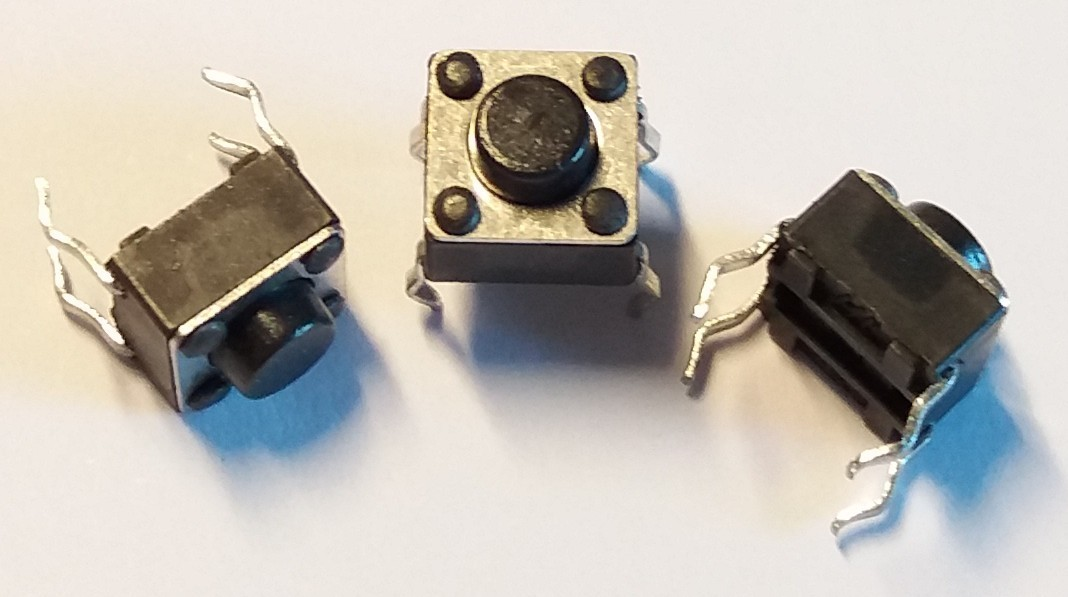
\includegraphics[width=0.25\textwidth]{pics/taster.jpg}
	\caption{Drei Taster.}
\end{wrapfigure}
Ein Taster ist wie ein Schalter, kann also geschlossen sein (Strom fließt) oder offen sein (Strom fließt nicht). Im Gegensatz zum Schalter springt ein Taster aber automatisch wieder in den offenen Zustand zurück, wenn er losgelassen wird.
 
In der unten abgebildeten Schaltplan ist dargestellt, wie man einen Taster am Arduino so anschließt, dass man seinen Zustand im digitalen Pin 3 auslesen kann.

\begin{aufgabe}\emph{Pulldown-Widerstand}
	
	Markiere die Kabel farbig, sodass die Kabel, die auf dem gleichen elektrischen Potential liegen, die gleiche Farbe haben. Notiere zudem den Wert des elektrischen Potentials.
\end{aufgabe}
\marginpar{%
	\textattachfile[description={Druckvorlage zu Kap. \thechapter, El. Potential an Tastern}]{./Auftraege/kap3-druckvorlage-taster.pdf}{
	\footnotesize%
	\drucker Vorlage%
	}%
	%\href{run:./Auftraege/kap3-druckvorlage-taster.pdf}{Vorlage}% ./ verweist auf das aktuelle Verzeichnis; ../ auf das übergeordnete
	\footnotesize%
	\\öffnen%
}

\begin{figure}[H]
	\hfill
	\begin{minipage}{0.4\textwidth}
		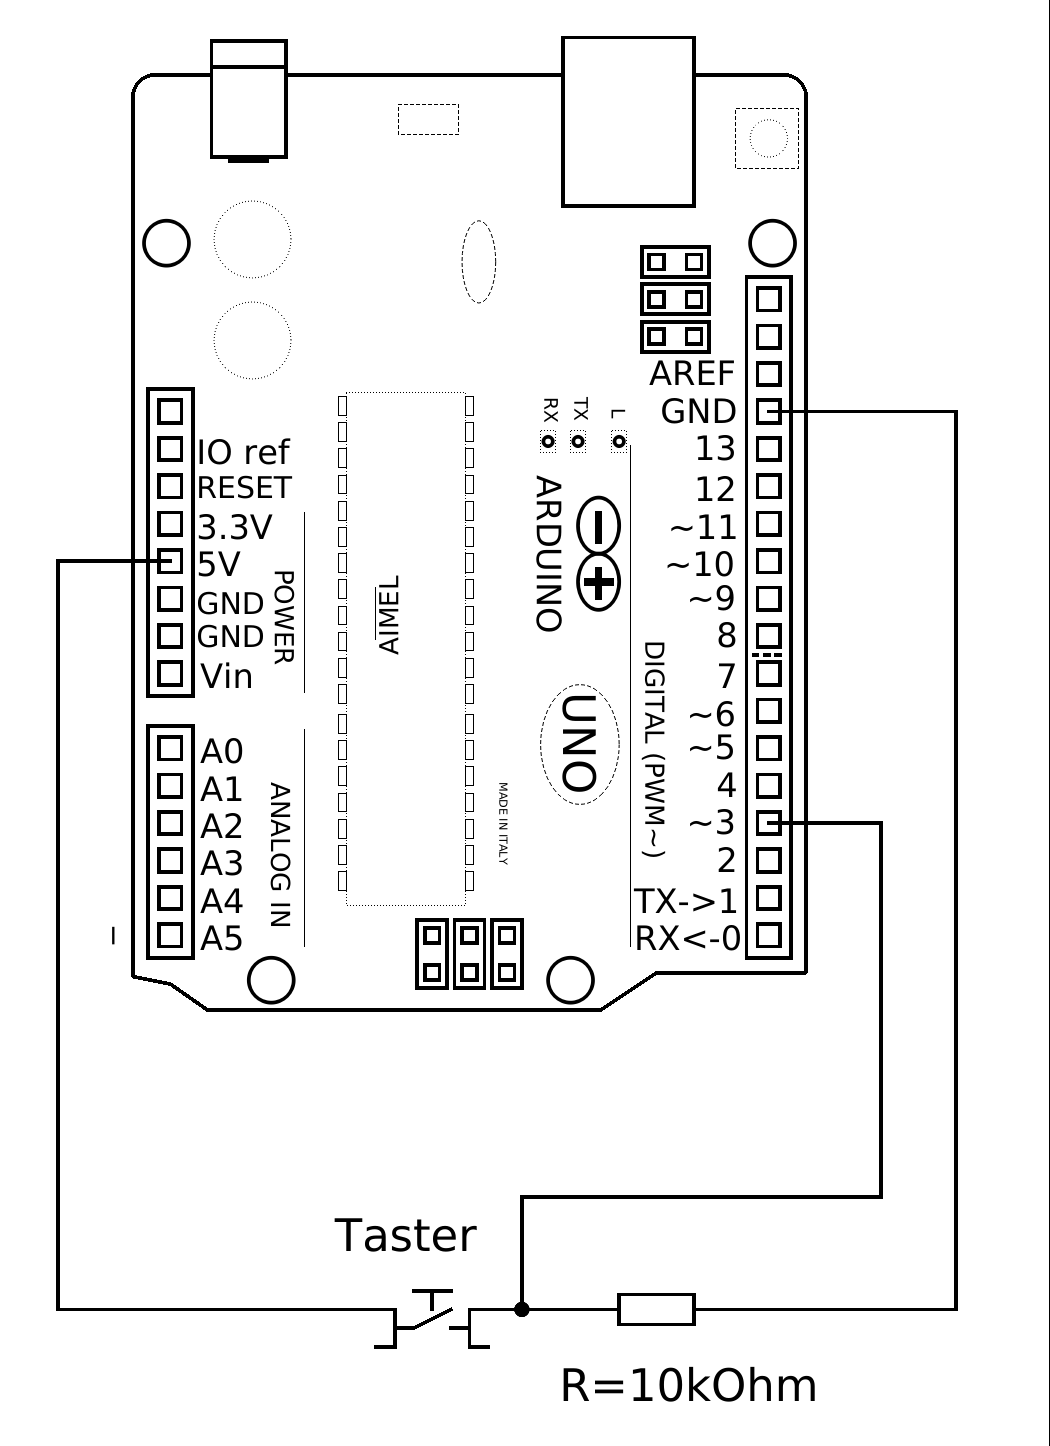
\includegraphics[width=0.8\textwidth]{Zeichnungen/taster-an-arduino.png}
		\caption{Taster offen (kein Stromfluss).}
	\end{minipage}
	\hfill
	\begin{minipage}{0.4\textwidth}
		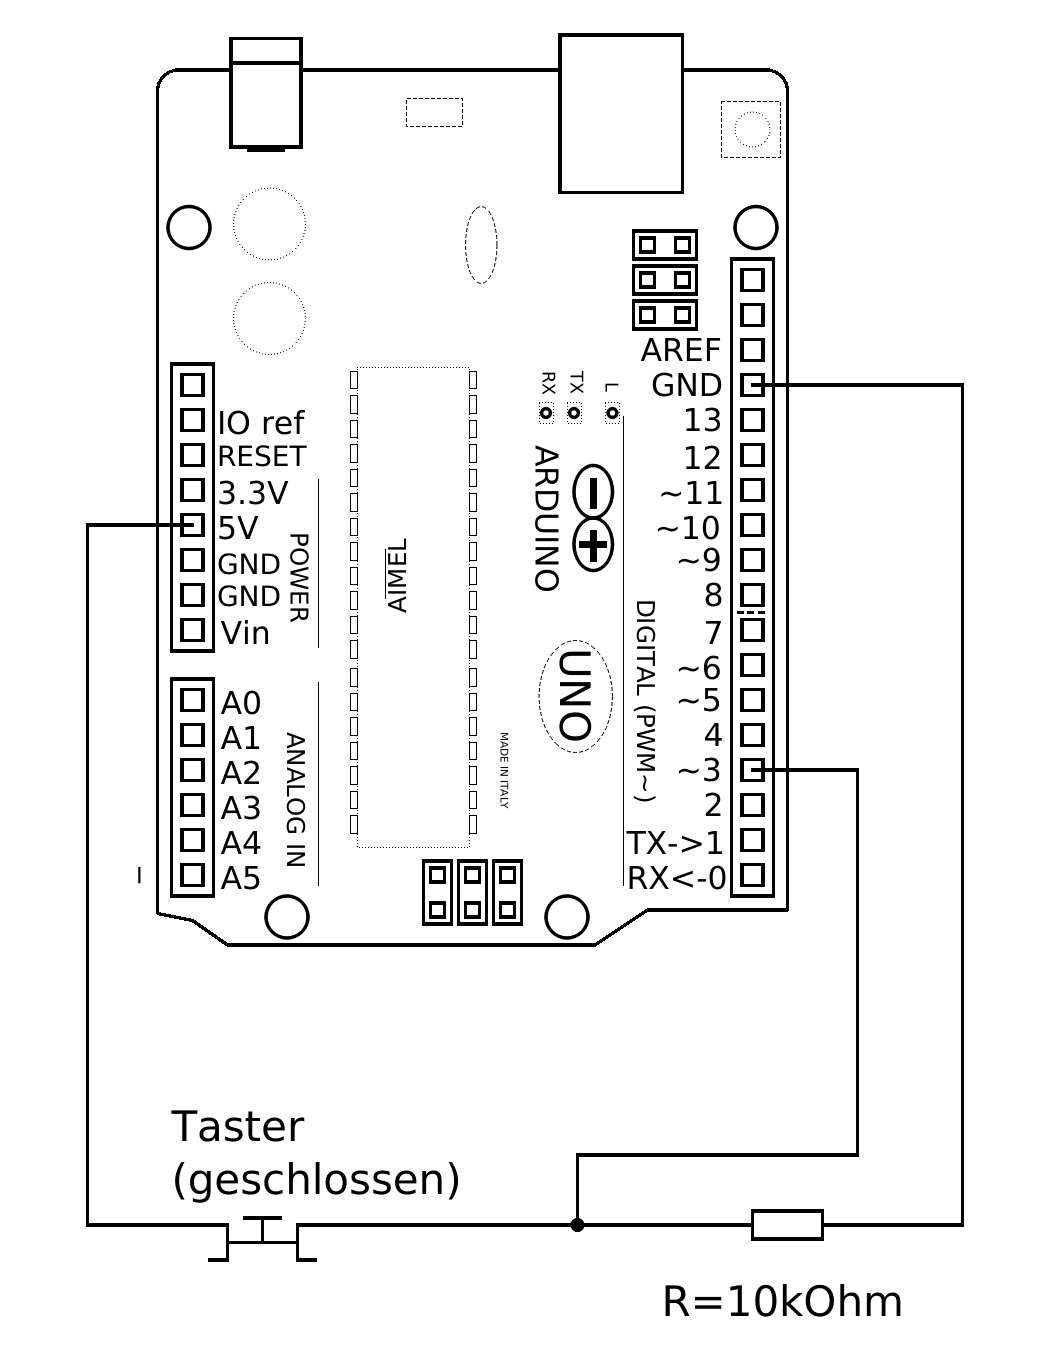
\includegraphics[width=0.8\textwidth]{Zeichnungen/taster-an-arduino-geschlossen.png}
		\caption{Taster geschlossen (Stromfluss).}
	\end{minipage}
	\hfill
	\label{abb:schaltplan-taster}
\end{figure}

\begin{zsfg}{Boolsche Werte einlesen} \label{sec:digitalread}
	Ein Potential von 5\,V wird im Programmcode auch als \texttt{HIGH}, \texttt{1} oder \texttt{TRUE} bezeichnet. Ein Potential von 0\,V wird im Programmcode auch als \texttt{LOW}, \texttt{0} oder \texttt{FALSE} bezeichnet. Ein digitaler Pin kann stets nur einen dieser beiden Zustände einnehmen. Potentiale von mehr als 1,4\,V werden stets als \texttt{HIGH} bzw. \texttt{TRUE} interpretiert.
	
	\begin{wrapfigure}{r}{0.25\textwidth}
		\centering
		
\includegraphics[width=0.25\textwidth]{pics/digitalread.png}
		\label{abb:digitalread}
	\end{wrapfigure}
	Dementsprechend hat der Befehl zum Einlesen des Potentials am digitalen Pin \emph{zwei mögliche Rückgabewerte}: \texttt{TRUE} oder \texttt{FALSE}. Das erkennt man auch an der eckigen Form das Befehls.
\end{zsfg}


\newpage
\begin{projekt}[Fußgängerampel]\label{proj:fussampel}
	\begin{wrapfigure}{r}{0.4\textwidth}
		\centering
		\vspace{-2\baselineskip}
		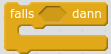
\includegraphics[width=0.15\textwidth]{pics/falls-dann.png}
		\label{abb:falls-dann}
	\end{wrapfigure}
	Baue und programmiere eine Fußgängerampel!
\end{projekt}
\marginpar{%
	\footnotesize%
	\werkzeug Neue \\
	Werkzeuge:\\
	\hyperref[sec:bewegungsmelder]{Bewegungs-\\melder}\\%
	\hyperref[sec:neigungsschalter]{Neigungs-\\schalter}
}

\begin{projekt}[Juke-Box]\label{proj:jukebox}
	\begin{wrapfigure}{r}{0.5\textwidth}
		\centering
		\vspace{-\baselineskip}
		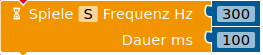
\includegraphics[width=0.5\textwidth]{pics/piezo-steuerung.png}
		\vspace{-\baselineskip}
		\label{abb:piezo-steuerung}
	\end{wrapfigure}
	Baue und programmiere eine Juke-Box!
	
	Die Juke-Box soll zwei verschiedene, kurze Melodien anspielen können.	
	(Zwei mögliche Beispiele mit Link zu den Noten: \href{https://www.lieder-archiv.de/alle\_meine\_entchen-notenblatt\_100055.html}{\enquote{Alle meine Entchen}}\footnote{\url{https://www.lieder-archiv.de/alle\_meine\_entchen-notenblatt\_100055.html}}, \href{https://www.lieder-archiv.de/o\_tannenbaum-notenblatt\_200078.html}{\enquote{Oh Tannenbaum}}\footnote{\url{https://www.lieder-archiv.de/o\_tannenbaum-notenblatt\_200078.html}}). 
	
	Dazu werden zwei Taster auf die beschriebene Art an zwei digitale Pins des Arduino angeschlossen. Schließe zudem an einen digitalen Pin einen Piezo-Summer an (siehe unten). 
	
	{\scriptsize Idee: Frick, Fritsch und Trick (2015): \emph{Einführung in Mikrocontroller - Der Arduino als Steuerzentrale}, Schülerforschungszentrum Bad Saulgau}
\end{projekt}

\begin{zsfg}{Piezo-Summer}

	\begin{minipage}{0.7\textwidth}
		Mit einem Piezo-Summer lassen sich Töne erzeugen, wenn man eine Spannung anschließt. Das lange Bein muss dabei an ein positives Potential angeschlossen werden; das kurze an ein negatives Potenzial bzw. GND. Ein Vorwiderstand ist dabei nicht notwendig, hilft aber die Lautstärke zu reduzieren.
	\end{minipage}
	\hfill
	\begin{minipage}{0.28\textwidth}
		\begin{minipage}{0.48\textwidth}
			\centering
			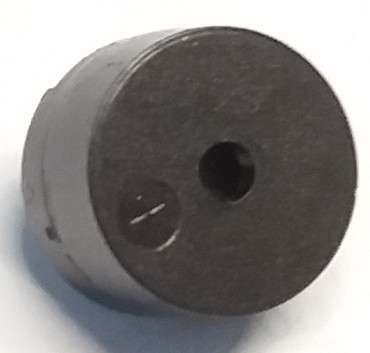
\includegraphics[width=0.9\textwidth]{./pics/piezo-summer.jpg}
		\end{minipage}
		\hfill
		\begin{minipage}{0.48\textwidth}
			\centering
			
\includegraphics[width=\textwidth]{./pics/piezo-schaltsymbol.png}
		\end{minipage}
	\end{minipage}
	
	\bigskip
	\emph{Funktionsweise:}\label{piezo-effekt}
	
	\begin{wrapfigure}{r}{0.4\textwidth}
		\vspace{-\baselineskip}
		\centering
		\begin{tikzpicture}[scale=0.7]
		\fill[white] (-0.2,-0.2) rectangle (8,4);
		%Kondensator links	
		\draw[gray!40,thick] (1.5,0.2) -- ++(0,-0.3) -- ++ (1.5,0);
		\fill[gray!40] (0,0.2) rectangle (3,0.5);
		\draw[gray!40,thick] (1.5,3.5) -- ++(0,0.3) -- ++ (1.5,0);
		\fill[gray!40] (0,3.2) rectangle (3,3.5);
		% Verbindungen/Sechseck
		\draw [thick] (1.5,0.8) -- (0.59,1.32) -- (0.58,2.36) -- (1.5,2.89) -- (2.39,2.36) -- (2.39,1.32) -- (1.5,0.8);
		%Ladungsverteilung
		\node at (1.5,0.8) [circle,fill=blue!50!white, draw, inner sep=1pt] (min1) {-};
		\node at (0.58,2.36) [circle,fill=blue!50!white, draw, inner sep=1pt] (min2) {-};
		\node at (2.39,2.36) [circle,fill=blue!50!white, draw, inner sep=1pt] (min3) {-};
		\node at (1.5,2.89) [circle,fill=red!50!white, draw, inner sep=1pt] (plus1) {\tiny +};
		\node at (0.59,1.32) [circle,fill=red!50!white, draw, inner sep=1pt] (plus2) {\tiny +};
		\node at (2.39,1.32) [circle,fill=red!50!white, draw, inner sep=1pt] (plus3) {\tiny +};
		%	
		%Kondensator rechts
		\draw[thick] (5.5,0.2) -- ++(0,-0.3) -- ++ (2,0) -- ++(0,1.9) ++(-0.2,0) -- ++(0.4,0);
		\fill[blue!40] (4,0.2) rectangle (7,0.5);
		\draw[thick] (5.5,3.5) -- ++(0,0.3) -- ++ (2,0) -- ++(0,-1.9) ++(-0.3,0) -- ++(0.6,0);
		\fill[red!40] (4,3.2) rectangle (7,3.5);
		\node at (7.8,2.2) {$U$};
		% Verbindungen/Sechseck rechts
		\draw [thick] (5.5,0.8) -- (4.59,1.12) -- (4.58,2.56) -- (5.5,2.89) -- (6.39,2.56) -- (6.39,1.12) -- (5.5,0.8);
		%Ladungsverteilung rechts
		\node at (5.5,0.8) [circle,fill=blue!50!white, draw, inner sep=1pt] (min11) {-};
		\node at (4.58,2.56) [circle,fill=blue!50!white, draw, inner sep=1pt] (min21) {-};
		\node at (6.39,2.56) [circle,fill=blue!50!white, draw, inner sep=1pt] (min31) {-};
		\node at (5.5,2.89) [circle,fill=red!50!white, draw, inner sep=1pt] (plus11) {\tiny +};
		\node at (4.59,1.12) [circle,fill=red!50!white, draw, inner sep=1pt] (plus21) {\tiny +};
		\node at (6.39,1.12) [circle,fill=red!50!white, draw, inner sep=1pt] (plus31) {\tiny +};
		\end{tikzpicture}
	\end{wrapfigure}
	In einem Piezo-Summer befindet sich ein Kristall mit unterschiedlichen Ladungsschwerpunkten, der von einem Kondensator umgeben ist. Wenn von außen an den Kristall eine Spannung angelegt wird, dann verformt sich die Kristallstruktur durch die Anziehung zwischen den Ladungsschwerpunkten und den Kondensatorplatten (\emph{\href{https://de.wikipedia.org/wiki/Piezoelektrizit\%C3\%A4t}{inverser piezo-elektrischer Effekt}}). Wenn keine Spannung anliegt, verformt sich der Kristall zurück. Durch diese Verformungen entstehen Druckwellen in der Luft, die wir als Ton wahrnehmen können.
\end{zsfg}
\vfill

\section{Vermischte Übungen}

\begin{aufgabe} \emph{Reihenschaltung}
	
	Eine rote LED soll an Pin 13 des Arduino betrieben werden. Durch die LED soll eine Stromstärke von $\SI{10}{\milli\ampere}$ fließen, was bei einer Spannung von $\SI{2,1}{\volt}$ an der LED der Fall ist. 
	\begin{enumerate}[label=\alph*), itemsep=0ex]
		\item Zeichne den zugehörigen Schaltplan.
		\item Berechne, wie groß der Vorwiderstand gewählt werden muss, damit diese Werte erreicht werden.
	\end{enumerate}
\end{aufgabe}

\begin{aufgabe} \emph{Parallelschaltung}
	
	Drei grüne LEDs sollen parallel geschaltet an Pin 13 des Arduino angeschlossen und mit einem gemeinsamen Vorwiderstand betrieben werden. Die LEDs halten eine Stromstärke von maximal $\SI{20}{\milli\ampere}$ bei einer Spannung von $\SI{3,3}{\volt}$ aus.
	
	\begin{enumerate}[label=\alph*), itemsep=0ex]
		\item Zeichne den zugehörigen Schaltplan.
		\item Ein Digitalpin am Arduino darf maximal mit einer Stromstärke von $\SI{40}{\milli\ampere}$ belastet werden. Berechne, welche Stromstärke dann maximal durch die einzelnen LEDs fließen darf.
		\item Der Tabelle unten kannst du den zugehörigen Spannungswert an den LEDs entnehmen. Berechne, wie groß der gemeinsame Vorwiderstand der LEDs sein muss, damit die in b) berechnete Stromstärke eingehalten wird.
		
		\begin{tabular}{c | c | c | c | c | c | c}
			\hline
			\textbf{Spannung U} & 3,03\,V & 3,07\,V & 3,1\,V & 3,13\,V & 3,16\,V & 3,19\,V \\ \hline
			\textbf{Stromstärke I} & 10\,mA & 11\,mA & 12\,mA & 13\,mA & 14\,mA & 15\,mA  \\ \hline
		\end{tabular}
	\end{enumerate}
\end{aufgabe}

\begin{aufgabe} \emph{Schaltung einer RGB-LED}
	
	\begin{wrapfigure}{r}{0.3\textwidth}
		\vspace{-\baselineskip}
		\centering
		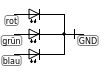
\includegraphics[width=0.2\textwidth]{./pics/rgb-led-schaltplan.png}
		\caption{Verschaltung der RGB-LED.}
		\vspace{-\baselineskip}
	\end{wrapfigure}
	Eine RGB-LED besteht aus drei einzelnen LEDs (rot, grün, blau), die jeweils über einen eigenen Digitalpin angesteuert werden (vgl. Schaltplan rechts). Am gemeinsamen GND-Anschluss soll ein gemeinsamer Vorwiderstand für alle LEDs angebracht werden, um die Stromstärke auf maximal $\SI{15}{\milli\ampere}$ zu begrenzen. Die Spannung an den LEDs sollte dann $\SI{2,25}{\volt}$ nicht überschreiten.
	\begin{enumerate}[label=\alph*), itemsep=0ex]
		\item Erkläre, welche Unterschiede zur Parallelschaltung von drei LEDs an \emph{einem} Digitalpin zu beachten sind.
		\item Berechne, wie groß der gemeinsame Vorwiderstand mindestens sein muss.
	\end{enumerate}
\end{aufgabe}

\newpage
\begin{aufgabe} \emph{Farbcodierung von Widerständen}
	
	\begin{enumerate}[label=\alph*), itemsep=0ex]
		\item Gib die Farbcodierung der folgenden Widerstandsgrößen an:
			\begin{multicols}{3}
				\begin{enumerate}[label=(\arabic*)]
					\item $\SI{330}{\ohm} \pm 1\%$,
					\item $\SI{10}{\kilo\ohm} \pm 2\%$,
					\item $\SI{4,7}{\kilo\ohm} \pm 10\%$.
				\end{enumerate}
			\end{multicols}
		\item Gib die Größe der folgenden Widerstände an:
			\begin{multicols}{2}
				\begin{enumerate}[label=(\arabic*)]
					\item \begin{tikzpicture}[scale=0.3]
							\shade [top color=lightgray, bottom color=gray] (-5,0.8) rectangle (10,1.2);
							\shade [top color=LightSkyBlue, bottom color=NavyBlue] (0,0) -- (5,0) arc [start angle=-135, end angle=135, radius=1.414] -- (0,2) arc [start angle=45, end angle=315, radius=1.414];
							\draw [fill=red] (0,0) rectangle ++(0.5,2);
							\draw [fill=red] (1,0) rectangle ++(0.5,2);
							\draw [fill=black] (2,0) rectangle ++(0.5,2);
							\draw [fill=black] (3,0) rectangle ++(0.5,2);
							\draw [fill=brown] (4.5,0) rectangle ++(0.5,2);
						 \end{tikzpicture}
					\item \begin{tikzpicture}[scale=0.3]
							\shade [top color=lightgray, bottom color=gray] (-5,0.8) rectangle (10,1.2);
							\shade [top color=LightSkyBlue, bottom color=NavyBlue] (0,0) -- (5,0) arc [start angle=-135, end angle=135, radius=1.414] -- (0,2) arc [start angle=45, end angle=315, radius=1.414];
							\draw [fill=green] (0,0) rectangle ++(0.5,2);
							\draw [fill=blue] (1,0) rectangle ++(0.5,2);
							\draw [fill=black] (2,0) rectangle ++(0.5,2);
							\draw [fill=yellow] (3,0) rectangle ++(0.5,2);
							\draw [fill=lightgray] (4.5,0) rectangle ++(0.5,2);
						 \end{tikzpicture}
				\end{enumerate}
			\end{multicols}
	\end{enumerate}
	\emph{Hinweis:} Als Hilfsmittel ist die Widerstandskarte aus den Boxen zugelassen.
\end{aufgabe}

\begin{aufgabe} \emph{Pullup-Widerstand}
	
	\begin{figure}[H]
		\centering
		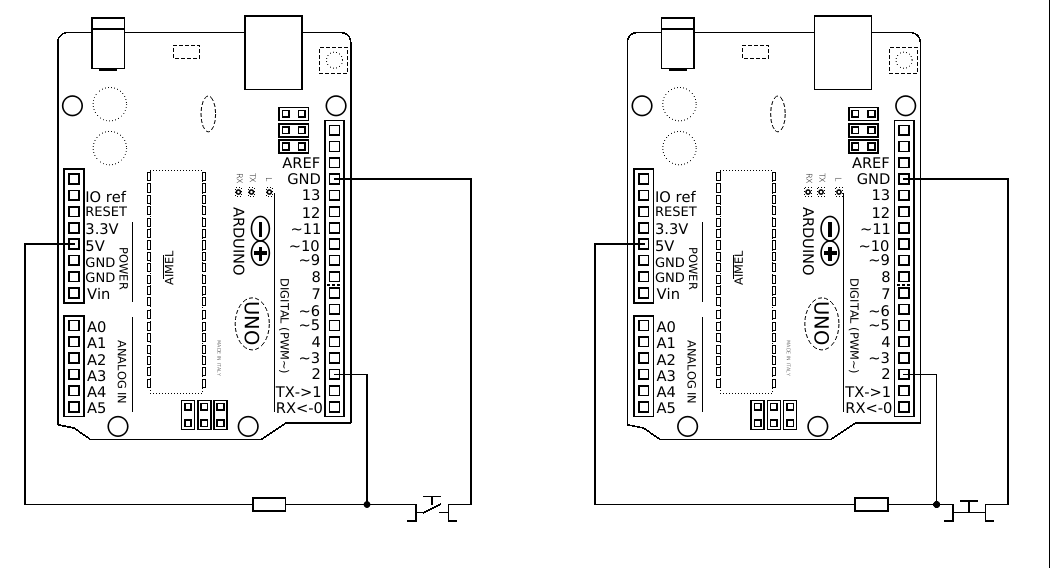
\includegraphics[width=0.8\textwidth]{./Zeichnungen/schaltplan-pullup.png}
	\end{figure}
	In der Abbildung wird ein Taster mit einem sogenannten Pullup-Widerstand an den Arduino angeschlossen. Links ist der Taster offen, rechts ist der Taster geschlossen.
	
	\bigskip
	\begin{minipage}{0.48\textwidth}
		\begin{enumerate}[label=\alph*), itemsep=0ex]
			\item Markiere die Kabel jeweils farbig, sodass die Kabel, die auf dem gleichen elektrischen Potential liegen, die gleiche Farbe haben. Notiere zudem den Wert des elektrischen Potentials.
			\item Erkläre, wie sich die Schaltung verhält, wenn das rechts abgebildete Programm auf dem Arduino läuft.
		\end{enumerate}
	\end{minipage}
	\hfill
	\begin{minipage}{0.5\textwidth}
		\centering
		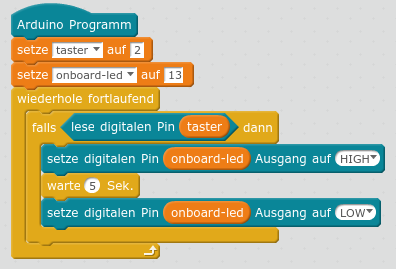
\includegraphics[width=0.9\textwidth]{./pics/programm-pullup-schaltung.png}
	\end{minipage}
\end{aufgabe}
\vfill


\begin{links}
	\item \href{https://www.youtube.com/watch?v=EbVmfGNwn0g}{FUTUREMAG}
	
	Kurze Dokumentation des FUTUREMAG zur Arduino-Welt
	
	\item \href{https://www.heise.de/make/meldung/Mehr-Komfort-der-Arduino-Ueberkopfwecker-4046184.html}{Arduino-Wecker}
	
	Mit einem selbst gebauten Wecker, der Uhrzeit und Alarmzeit getrennt voneinander anzeigt, erfüllte ein Bastler seinen Wunsch nach mehr Komfort.
	
	\item \href{https://www.instructables.com/id/Aquarium-LED-Controller/}{Aquarium-Licht}
	
	Der Bastler hinter diesem Projekt wollte seinen Fischen im Aquarium ein natürliches Licht einschließlich Sonnenaufgang, Sonnenuntergang und Nacht gönnen. Auf die gleiche Art und Weise kann man natürlich auch sein Terrarium beleuchten.
	
	\item \href{https://www.heise.de/make/meldung/Kein-Geld-fuer-eine-Oculus-Rift-VR-Brille-selbstgebaut-3949507.html}{VR-Brille}
	
	Drei Schüler aus Frankreich hatten kein Geld für eine Virtual Reality Brille – aber dafür das Know How, um sich mit einem Arduino und einem Gehäuse aus dem 3D-Drucker selbst eine VR-Brille zu basteln.
\end{links}
	
\chapter{Konzepte der Informatik: Bausteine von Algorithmen}

Mit den digitalen Pins, die sich als Ausgänge und Eingänge nutzen lassen, lassen sich zahlreiche Projekte umsetzen. Allerdings wird die Programmierung schnell unübersichtlich oder unnötig aufwendig, wenn man sich nicht mit algorithmischen Strukturen auskennt. Daher geht es im folgenden Kapitel um die Einführung von grundlegenden algorithmischen Bausteinen.

\bigskip
In diesem Kapitel lernst du\dots
\begin{itemize}
	\item \dots Variablen zu benutzen,
	\item \dots mit Schleifen effizient zu programmieren,
	\item \dots zufällige Ereignisse zu programmieren,
	\item \dots den Arduino mit dem Computer kommunizieren zu lassen,
	\item \dots überblicksweise, wie die USB-Verbindung funktioniert,
	\item \dots was es mit den berühmten Einsen und Nullen auf sich hat,
	\item \dots wie man Programme zur Planung oder zum Vergleich auf Papier einfach darstellen kann.
\end{itemize}

\bigskip

\begin{projektueberblick}
	\item Auto-Blinker \dotfill \pageref{proj:blinker}
	\item Bombe bauen \dotfill \pageref{proj:bombe}
	\item Reaktionszeitmesser \dotfill \pageref{proj:reaktionszeitmesser}
\end{projektueberblick}

\newpage
\section{Programme mit Variablen strukturieren}
% Variablen strukturieren Programme: Vergleich von Programm mit und ohne Variablen
% -> Vorstellung als Koffer; Zeichnung mit Verweis auf Speicherfläche
% -> sinnvolle Benennung von Variablen
\vspace{-0.5\baselineskip}
\begin{aufgabe}
	Jonas und Jana haben jeweils LEDs an die Pins 13 bis 11 angeschlossen und steuern diese mit den unten abgebildeten Programmen. Vergleiche die beiden Programme im Hinblick auf ihre Wirkung und die Art der Programmierung. Welches gefällt dir besser?
	
	Zusatzüberlegung: Wie viel muss man ändern, wenn man zum Beispiel Probleme mit Pin 13 hat und deshalb die zugehörige LED an Pin 10 anschließen will?
\end{aufgabe}
\marginpar{%
	\textattachfile[description={Folie zu Kap. \thechapter, Variableneinsatz}]{./Auftraege/kap4-auftrag-variablen.pdf}{%
		\footnotesize\folie Folie %
	}%
	\footnotesize%
	%\folie \href{run:./Auftraege/kap4-auftrag-variablen.pdf}{Folie}\\%
	\\öffnen%
}

\vspace{-0.75\baselineskip}
\begin{figure}[H]
	\begin{minipage}{0.48\textwidth}
		\centering
		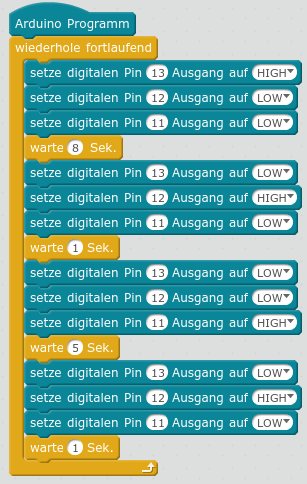
\includegraphics[width=0.75\textwidth]{pics/ampel-ohne-variablen.png}
		\caption{Jonas Programm zum Steuern der LEDs.}
	\end{minipage}
	\hfill
	\begin{minipage}{0.48\textwidth}
		\centering
		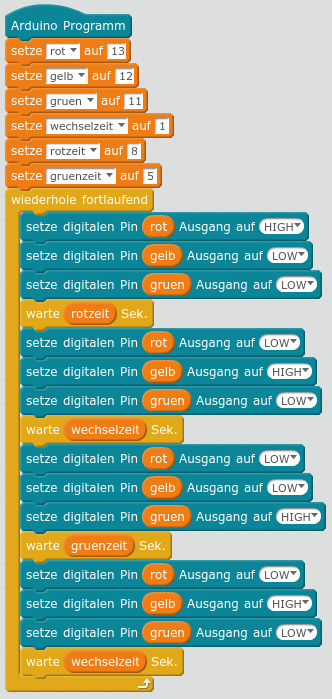
\includegraphics[width=0.75\textwidth]{pics/ampel-mit-variablen.png}
		\caption{Janas Programm zum Steuern der LEDs.}
	\end{minipage}
\end{figure}
\vspace{-0.75\baselineskip}

\begin{zsfg}{Variablen}
	\begin{wrapfigure}{r}{0.25\textwidth}
		\begin{tikzpicture}[scale=0.5]
		\draw (-0.2,0) -- (3.2,0);
		\draw (-0.2,1) -- (3.2,1);
		\draw [fill=white] (0,0) rectangle (1,1);
		\draw [fill=white] (1,0) rectangle (2,1);
		\draw [fill=white] (2,0) rectangle (3,1);
		\node (rot) at (1.5,0.5) {\sffamily rot};
		\draw (3.8,0.5) -- (3.8,-4);
		\draw (6.2,0.5) -- (6.2,-4);
		\draw [fill=gray!40] (3.8,-1) rectangle (6.2,-3.5);
		\node (wert) at (5,-2.25) {\sffamily 13};
		\draw [gray!30!black, thick,->] (rot) to [out=270,in=140] (wert);
		\node at (5,-3) {\sffamily\scriptsize Speicher};
		\end{tikzpicture}
	\end{wrapfigure}
	Eine Variable kann man sich als Koffer vorstellen, der einen Namen bekommt und in dem man einen Zahlenwert oder ein Wort speichert. Jedes Mal, wenn der Name des Koffers aufgerufen wird, wird der abgespeicherte Wert hervorgeholt und an die Stelle des Namens gesetzt.	
	Intern wird der Variablenname als Verweis auf einen bestimmten Speicherplatz genutzt, in dem der Wert der Variable abgelegt ist.
	
	Wir unterscheiden drei \textbf{Datentypen}, die in Variablen abgespeichert werden: Zahlen (runde Felder), Zeichen (rechteckige Felder) und Wahrheitswerte (spitze Felder: Wahr oder falsch). Wahrheitswerte werden auch \emph{boolsche Variablen} genannt.
\end{zsfg}

% Variablen:
% die beiden Programme von Jonas und Jana bewirken das Gleiche (Ampelschaltung)
% Jonas Programm ist kürzer
% Janas Programm ist verständlicher, weil sie Variablen einsetzt, deren Name die Funktion verdeutlicht
% Janas Programm ist praktischer, weil man bei einer Änderung eines Pins oder einer Pause das Programm nur an einer Stelle ändern muss

\section{Lauflichter effizient programmieren}

Lauflichter findet man inzwischen überall in unserer Welt: An den Rändern von Landebahnen an Flughäfen, an Spieleautomaten, aufdringlichen Werbeschildern, als Blinker von modernen Autos und vieles mehr.

\begin{ziel}
	\textbf{Ziel:} Ein Auto-Blinker soll auf möglichst effiziente Weise programmiert werden.
\end{ziel}

\begin{aufgabe}
	Fange mit einem einfachen Lauflicht an und baue dieses immer weiter aus.
	\begin{enumerate}[label=\alph*), itemsep=0ex, parsep=0ex]
		\item Bringe vier LEDs mit Vorwiderständen von $330\,\Omega$ an den Pins 10 bis 13 an. Programmiere sie so, dass sie nacheinander aufleuchten und wieder ausgehen. Nutze für die Pausenzeit eine Variable.
	\end{enumerate}
	\begin{minipage}{0.76\textwidth}
		\begin{enumerate}[label=\alph*), itemsep=0ex, parsep=0ex,start=2]
			\item Du wirst leicht erkennen, dass sich die Schritte zum Aufleuchten und Ausstellen bei jeder LED wiederholen. Sie lassen sich effizienter mit einer Wiederholungsschleife programmieren, die aber nicht unendlich lange weiterläuft. 
			
			Lege eine Laufvariable namens \button{pin} an, die für die Angabe des Pins genutzt wird, der an bzw. ausgestellt werden soll. In jedem Schleifendurchlauf muss die \button{pin}-Variable dann entsprechend geändert werden.
			
			Programmiere das Lauflicht aus a) mithilfe einer Laufvariable und einer Wiederholungsschleife möglichst effizient.
		\end{enumerate}
	\end{minipage}
	\hfill
	\begin{minipage}{0.22\textwidth}
		\begin{figure}[H]
			\centering
			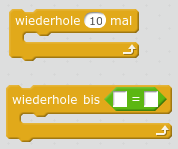
\includegraphics[width=\textwidth]{pics/schleifenvarianten.png}
			\caption{Mögliche Schleifen für Teil b.}
		\end{figure}
	\end{minipage}
	\marginpar{%
		\textattachfile[description={Arbeitsblatt zu Kap. \thechapter, Trace-Tabelle}]{./Auftraege/kap4-trace-tabelle.pdf}{%
		\ausrufezeichen%
		}%
		\footnotesize%
		%\ausrufezeichen 
		\\Trace-Tabelle
	}
	\begin{enumerate}[label=\alph*), itemsep=0ex, parsep=0ex,start=3]
		\item \emph{Für Schnelle:} Ergänze weitere LEDs und passe dein Programm daran an.
	\end{enumerate}
\end{aufgabe}

\begin{aufgabe}
	Programmiere ein Lauflicht, das hin- und zurückläuft.
\end{aufgabe}

\marginpar{%
	\footnotesize%
	\video \\
	\href{https://www.youtube.com/watch?v=s317_5aFL6E}{Blinker-Beispielvideo}
}
\begin{projekt}[Auto-Blinker]\label{proj:blinker}
	Programmiere ein Lauflicht so, wie es auch als Blinker in modernen Autos genutzt wird.
\end{projekt}

\begin{zsfg}{Schleifen}
	
	Bei der Programmierung werden häufig Schleifen genutzt, die die Anweisungen in ihrem Rumpf (oder Körper) solange wiederholen, bis eine gewisse Abbruchbedingung eintritt.
	
	\emph{Zählschleifen} wiederholen die Anweisungen im Rumpf für eine festgelegte Anzahl von Wiederholungen.
	
	Die \texttt{wiederhole bis}-Schleife wiederholt die Anweisungen solange, bis die angegebene Bedingung wahr ist. Zum Beispiel lässt sich mit dem grünen Block für den Vergleich zweier Zahlen eine \texttt{WAHR}/\texttt{FALSCH}-Aussage erzeugen, wie man an der eckigen Form erkennt. Ein weiteres Beispiel ist der Block \texttt{lese digitalen Pin}, der ebenfalls eine \texttt{WAHR}/\texttt{FALSCH}-Aussage erzeugt (vgl. S.\,\pageref{sec:digitalread}). Die Überprüfung, ob die Bedingung wahr ist, erfolgt hier \emph{vor} der Ausführung der Befehle im Rumpf. Daher nennt man die Schleife auch \emph{kopfgesteuert}.
\end{zsfg}

\newpage
\section{Zufällige Ereignisse programmieren}

\begin{wrapfigure}{r}{0.2\textwidth}
	\centering
	
\includegraphics[width=0.18\textwidth]{pics/zufallszahl.png}
\end{wrapfigure}
Viele Dinge werden interessanter, wenn sie sich nicht immer auf die genau gleiche Art wiederholen. Für diese Fälle kann man im Programm den grünen Block für Zufallszahlen verwenden, der jedes Mal eine neue Zufallszahl erzeugt, wenn er aufgerufen wird. Ein einfaches Beispiel ist die \enquote{Bombe}, die man bei dem Spiel \enquote{Tick Tack Bumm} startet und die man so lange herum geben muss, bis sie explodiert. Dabei ist die Dauer des Tickens ein zufälliger Wert zwischen ca. 5\,s und 20\,s.
\marginpar{%
	\footnotesize%
	\video \\
	\href{https://el-voss.de/downloads/ticktack.html}{Bomben-Beispielvideo}
}
\marginpar{%
	\footnotesize%
	\textattachfile[description={Arbeitsblatt zu Kap. \thechapter, Bombenprogramm}]{./Auftraege/kap4-bombenvergleich.pdf}{
	\footnotesize%
	\ausrufezeichen}%
	\\Programm-%
	\\vergleich
}

\medskip
\begin{projekt}[Bombe bauen]\label{proj:bombe}
	Baue und programmiere eine \enquote{Bombe}, die für eine zufällige Dauer zwischen 5\,s und 20\,s tickt und dann explodiert. Die Bombe wird über einen Taster aktiviert.
\end{projekt}
\vspace{-\baselineskip}

\section{Kommunikation mit dem Arduino: Der serielle Monitor}
\label{sec:seriellermonitor}
%Reaktionszeitmesser mit Zufallselement; Aufgabe: Struktogramm
Bisher hatte die Kommunikation mit dem Arduino stets nur eine Richtung: Vom Computer zum Arduino. Das reicht nicht mehr, wenn der Arduino etwas messen und dem Anwender dann mitteilen soll, was er gemessen hat. Für solche Fälle ist der serielle Monitor die einfachste Kommunikationsmöglichkeit zwischen Arduino und Computer.

\begin{ziel}
	\textbf{Frage:} Wie kann der Arduino mit dem Computer kommunizieren?
\end{ziel}

\begin{wrapfigure}{r}{0.25\textwidth}
	\centering
	
\includegraphics[width=0.23\textwidth]{pics/serialprint.png}
\end{wrapfigure}
Mit dem Block \button{Sende Text an seriellen Port} kann der Arduino angewiesen werden, den eingegebenen Text über die serielle Schnittstelle an den Computer zu senden. Der Text kann auch eine Zahl sein - diese Zahl wird dann eben nicht mehr als Zahl, sondern als Text behandelt und ausgegeben. Am Computer sieht man das Ergebnis im Fenster unten rechts, in dem bisher bereits Statusnachrichten zur Übertragung des Programms auf den Arduino zu sehen waren. \emph{Hier muss der Zeichenmodus eingestellt werden, damit die Daten für uns lesbar sind.}

\begin{projekt}[Reaktionszeitmesser]\label{proj:reaktionszeitmesser}
	Baue und programmiere einen Reaktionszeitmesser.
	
	\begin{wrapfigure}{r}{0.2\textwidth}
		\centering
		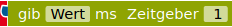
\includegraphics[width=0.18\textwidth]{pics/stoppuhr.png}
	\end{wrapfigure}
	Der Reaktionszeitmesser soll zunächst warten, bis ein Taster gedrückt wurde, der besagt, dass es losgehen kann. Dann wird eine LED angeschaltet (Vorwiderstand!) und nach einer zufälligen Zeit wieder ausgeschaltet. Nun beginnt die Zeitmessung. Die Stoppuhr läuft solange, bis der Taster gedrückt wurde. Die gemessene Zeit wird dann über den seriellen Monitor ausgegeben und es wird erneut gewartet, bis der Anwender bestätigt, dass es losgehen kann.
	
	Miss mindestens zehn Mal deine Reaktionszeit und bestimme den Mittelwert. Bist du besser als dein Partner?
	
	\emph{Für Schnelle:} Nutze den \button{Verbinde <\_> mit <\_>}-Block, um der Ausgabe folgende Form zu geben: \enquote{Deine Reaktionszeit: 10s}.
	
	{\scriptsize Idee: Frick, Fritsch und Trick (2015): \emph{Einführung in Mikrocontroller - Der Arduino als Steuerzentrale}, Bad Saulgau}
\end{projekt}

\begin{zsfg}{Serielle Schnittstellen}
	
	\begin{wrapfigure}{r}{0.5\textwidth}
		\centering
		\begin{tikzpicture}[scale=0.5]
		\fill [white] (-4,-0.7) rectangle (8,3.2);
		\foreach \x in {1,...,7} \draw [dashed] (\x,-0.5) -- (\x,2.5);
		\draw (0,0) -- (1,0) -- (1,2) -- (2,2) -- (2,0) -- (3,0) -- (3,2) -- (6,2) -- (6,0) -- (8,0);
		\foreach \b in {0,2,6,7} \node at (\b+0.5,-0.4) {\sffamily\scriptsize 0};
		\foreach \b in {1,3,4,5} \node at (\b+0.5,-0.4) {\sffamily\scriptsize 1};
		\draw [{<[length=3pt, width=5pt]}-{>[length=3pt, width=5pt]}] (1,2.2) -- (2,2.2) node at (1.5,2.7) {\sffamily\scriptsize $8,68\,\mu s$};
		\node at (-2,0) {\sffamily \scriptsize logisch 0 / 0\,V};
		\node at (-2,2) {\sffamily \scriptsize logisch 1 / 5\,V};
		\end{tikzpicture}
		\caption{Durch ein gepulstes elektrisches Potential wird eine Folge von Bits zwischen Arduino und Computer übertragen.}
		\vspace{-\baselineskip}
	\end{wrapfigure}
	Bei seriellen Schnittstellen werden die Bits, also die Einsen und Nullen nacheinander (seriell) von einem Gerät zum nächsten geschickt. Dazu werden el. Potenzialpulse mit einer festgelegten Länge von einem Gerät gesendet und vom anderen Gerät empfangen. Dabei kann ein Puls mit 5V als eine 1 und ein Puls von 0V als eine 0 interpretiert werden. In unserem Fall ist eine Bitrate von 115200 Bit pro Sekunde festgelegt, wodurch ein Bit bzw. Potenzialpuls $\SI{8,68}{\micro\second}$ dauert.
	
	\begin{wrapfigure}{r}{0.3\textwidth}
		\centering
		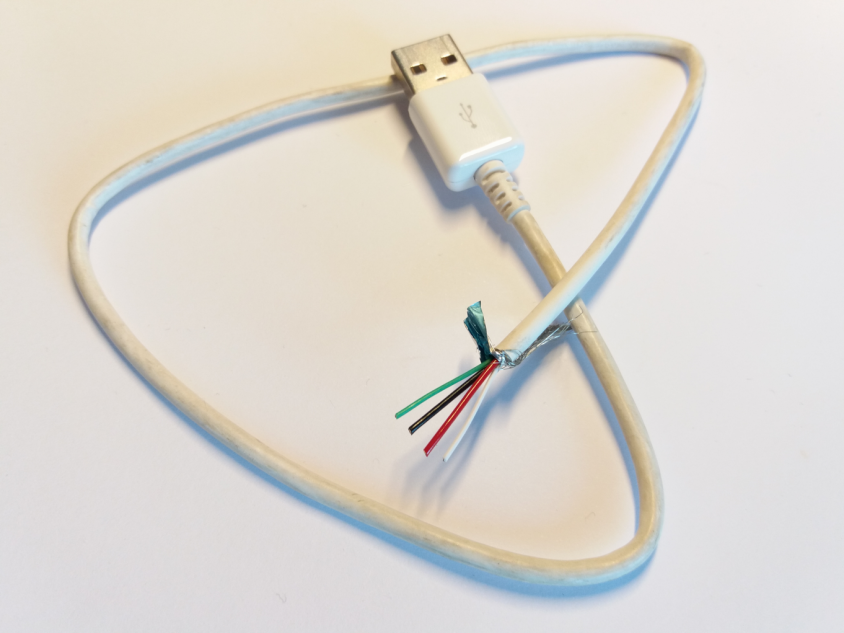
\includegraphics[width=0.3\textwidth]{pics/usbkabel-qn.png}
		\caption{Ein USB-Kabel enthält vier Leitungen.}
		\vspace{-\baselineskip}
	\end{wrapfigure}
	Die bekannteste serielle Schnittstelle ist USB - der \emph{Universal Serial Bus}. Für die Kommunikation werden vier Kabel benötigt, die man erkennen kann, wenn man das USB-Kabel durchschneidet: Das schwarze Kabel (GND) und das rote Kabel (5\,V) stellen die Spannungsversorgung sicher. Dazu kommt eine Empfängerleitung (RX) und eine Senderleitung (TX). Der Empfängerpin des Arduino ist Pin 0 und muss mit dem Senderpin am Computer verbunden sein. Umgekehrt muss der Senderpin des Arduino (Pin 1) mit dem Empfängerpin am Computer verbunden sein. Wenn etwas an Pin 0 oder 1 des Arduino angeschlossen ist, kann es passieren, dass die Übertragung eines neuen Programms auf den Arduino nicht funktioniert, weil das angeschlossene Bauteil das richtige Setzen der Potentialpulse verhindert.
\end{zsfg}

\begin{aufgabe}
	Angenommen, du hast ein Programm erstellt, das 75\,kB groß ist. Berechne, wie lange es bei einer Bitrate von 115200 Bit pro Sekunde dauert, diese Datenmenge auf den Arduino zu übertragen.
	
	\emph{Hinweise:} 1\,kB = 1 kilo Byte = 1000 Byte, 1 Byte = 8 Bit
\end{aufgabe}
%75kB = 75000B=600000 bit; bei 8,68 microsekunden pro Bit macht das insgesamt 5208000mikrosekunden =5,208 Sekunden

\subsection{Exkurs: Zufallszahlen von Mikrocontrollern/-prozessoren}
% Ausgabe von Zufallszahlen auf seriellem Monitor, dann Reset -> immer die gleichen (gilt auch für TR oder PC)

\marginpar{%
	\footnotesize%
	\werkzeug Neues \\
	Werkzeug:\\
	\hyperref[sec:ultraschallsensor]{Ultraschall-\\sensor}%
}
\begin{aufgabe}
	
	\begin{wrapfigure}{r}{0.5\textwidth}
		\centering
		\vspace{-\baselineskip}
		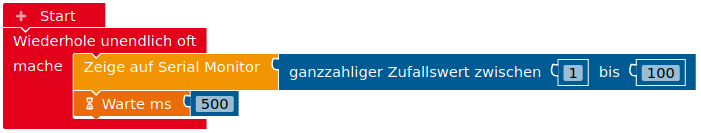
\includegraphics[width=0.5\textwidth]{pics/zufallszahlengenerator.png}
	\end{wrapfigure}
	Übertrage das rechts abgebildete Programm auf den Arduino und betrachte die so erzeugten Zufallszahlen. Drücke dann auf den Reset-Taster am Arduino und betrachte die nun erzeugten Zufallszahlen. Wiederhole den Vorgang einige Male und beschreibe Auffälligkeiten.
\end{aufgabe}

\newpage
\section{Kurze Einführung in die Codierung von Zahlen und Zeichen}
Wie wir gesehen haben, können der Computer und der Arduino nur die berühmten Einsen und Nullen austauschen.

\begin{ziel}
	\textbf{Frage:} Wie ist es möglich, mithilfe von Einsen und Nullen Zahlen und Zeichen darzustellen?
\end{ziel}

\subsection{Ein Einblick ins Binärsystem}\label{sec:binaer}

\begin{aufgabe}
	\begin{enumerate}[label=\alph*), noitemsep]
		\item Erkläre die unten dargestellte Zerlegung der Zahl 1509 im Dezimalsystem:
		\vspace{-0.5\baselineskip}
		\begin{align*}
		1509 &= 1\cdot 1000 + 5 \cdot 100 + 0\cdot 10 + 9 \cdot 1 \\
		&= 1\cdot 10^3+ 5\cdot 10^2 + 0 \cdot 10^1 + 9 \cdot 10^0
		\end{align*}
		\vspace{-1.5\baselineskip}
		\item Das Binärsystem arbeitet mit Zweierpotenzen statt Zehnerpotenzen. Notiere alle Zweierpotenzen von $2^0$ bis $2^{10}$. Erkläre kurz, wieso es bei der Verwendung von Zweierpotenzen nur die Ziffern $0$ und $1$ geben kann.
		\item Übersetze die Zahlen vom Binärsystem ins Dezimalsystem:
		\vspace{-0.5\baselineskip}
		\begin{multicols}{3}
			\begin{enumerate}[label=(\arabic*),noitemsep]
				\item 1011
				\item 11000001
				\item 01010101
			\end{enumerate}
		\end{multicols}
		\vspace{-0.5\baselineskip}
		\item Finde die Binär-Darstellungen von 12, 21 und 127.
		\item Ein Byte besteht aus acht Bit, also acht Nullen oder Einsen. Bestimme, wie viele verschiedene Zahlen man damit darstellen kann.
	\end{enumerate}
\end{aufgabe}

\marginpar{%
	\footnotesize%
	\werkzeug Neues \\
	Werkzeug:\\
	\hyperref[sec:lcd]{LC-Display}%
}
Für negative Zahlen und Zahlen mit Komma braucht man noch einige zusätzliche Kniffs, die an dieser Stelle zu weit führen.

\medskip
\begin{zsfg}{Das Binärsystem}
	
	Im Gegensatz zum Dezimalsystem zur Basis 10 mit Ziffern von 0 bis 9 arbeitet das Binärsystem zur Basis 2 mit den Ziffern 0 und 1.
	
	Im Binärsystem wird jede Zahl durch die Potenzen von 2 zusammengesetzt. Die Binärzahl \texttt{1001} bedeutet dann so viel wie $\texttt{1}\cdot 2^3 + \texttt{0}\cdot 2^2+ \texttt{0}\cdot 2^1 + \texttt{1}\cdot 2^0$. Den Wert der Binärzahl im Dezimalsystem erhält man dann durch eben diese Rechnung: $\texttt{1}\cdot 2^3 + \texttt{0}\cdot 2^2+ \texttt{0}\cdot 2^1 + \texttt{1}\cdot 2^0= 8 + 0 + 0 + 1 = 9$.
	
	Da bei Binärzahlen wie \texttt{1001} nicht sofort ersichtlich ist, ob es sich um eine Binärzahl oder eine Dezimalzahl handeln soll, wird der Zahl häufig ein \texttt{0b} vorangestellt: \texttt{0b1001}. Ebenfalls üblich ist es, die Basis im Index zu notieren: $\texttt{1001}_{2}$ zeigt eine Binärzahl an; $1001_{10}$ eine Dezimalzahl.
	
	Um die Binärdarstellung einer Dezimalzahl wie z.\,B. 13 zu finden, geht man folgendermaßen vor:
	
	\begin{minipage}{0.65\textwidth}
		\begin{enumerate}[noitemsep]
			\item Finde die größte Zweierpotenz, die in die Dezimalzahl passt. Notiere dafür eine \texttt{1}.
			\item Überprüfe, wie oft die nächstkleinere Zweierpotenz in den Rest passt. Notiere entsprechend eine \texttt{0} (passt nicht) oder eine \texttt{1} (passt einmal).
			\item Wiederhole den Schritt (2), bis kein Rest mehr übrig ist.
		\end{enumerate}
	\end{minipage}
	\hfill
	\begin{minipage}{0.34\textwidth}
		\begin{align*}
			13 &= 1\cdot 8 + 5 & \texttt{1~~~} \\
			5 &= 1\cdot 4 + 1 & \texttt{11~~} \\
			1 &= 0\cdot 2 +1 & \texttt{110~} \\
			1&= 1\cdot 1 & \texttt{1101} 
		\end{align*}
		\vspace{1\baselineskip}
	\end{minipage}
	\vspace{-\baselineskip}
\end{zsfg}

\subsection{Ein Einblick in die ASCII-Tabelle}
Auf diese Codierung im Binärsystem wird dann zurückgegriffen, wenn die übertragenen (bzw. abgespeicherten) Daten vom Typ \enquote{Zahl} sind. Wie man an der eckigen Form des Arguments im Block \button{Sende Text an seriellen Port} sieht, werden dabei aber Daten vom Typ \enquote{Zeichen} übertragen. Um welches Zeichen es sich handelt, lässt sich nicht allein anhand der Bits schlussfolgern, sondern muss durch einen Standard festgelegt werden. Der einfachste Standard ist der ASCII-Standard, der später in den Unicode- und schließlich in den UTF-8-Standard eingeflossen ist.

\begin{zsfg}{Der ASCII-Code}
	Der \href{http://www.computer-masters.de/ascii-tabelle.php}{American Standard Code for Information Interchange (ASCII)} legt durch eine Tabelle für 128 Zeichen fest, wie diese mithilfe von sieben Bits codiert werden. Wenn man diese Bitfolge nicht als Zeichen, sondern als Zahl interpretiert, kann man jedem Zeichen eine Zahl zuordnen, die diesem entspricht. Zum Beispiel wird der Buchstabe A durch die Folge 1000001 codiert und entspricht damit der Zahl 65.
\end{zsfg}

\begin{aufgabe}
	Finde und notiere die ASCII-Bitfolgen zu den Zeichen \enquote{V}, \enquote{s}, \enquote{+}, \enquote{?} und \enquote{0}.
	
	ASCII-Tabelle: \url{http://www.computer-masters.de/ascii-tabelle.php}
\end{aufgabe}

\begin{recherche}{Von ASCII über Unicode zu UTF-8}
	Der ASCII-Standard ist ausreichend, wenn man nur englische Texte darstellen muss. In anderen Sprachen ergibt sich jedoch die Herausforderung, weitere Zeichen codieren zu müssen und spätestens mit der Verbreitung des Internets und der weltweiten Kommunikation war das auch für englischsprachige Programmierer relevant. Eine locker geschriebene Einführung zur Entwicklung der unterschiedlichen Standards gibt der Artikel \href{https://www.joelonsoftware.com/2003/10/08/the-absolute-minimum-every-software-developer-absolutely-positively-must-know-about-unicode-and-character-sets-no-excuses/}{The Absolute Minimum Every Software Developer Absolutely, Positively Must Know About Unicode and Character Sets (No Excuses!)}.
	
	\emph{Hilfreich für das Verständnis des Artikels ist die Kenntnis von Hexadezimalzahlen (s. S. \pageref{proj:rgbled2} f.).}
\end{recherche}

\newpage
\section{Programme mit Struktogrammen darstellen}
Wenn wir uns über Programme austauschen, dann haben wir nicht immer den Computer zur Hand. In solchen Momenten wäre es viel zu aufwendig, die bunten Blöcke von mBlock zu malen. Außerdem könnte es sein, dass jemand anderes das Programm nicht mit Blöcken, sondern mit Text in der Programmiersprache C++ aufschreiben will, also so wie es in der rechten Seite von mBlock abgebildet ist.

\begin{ziel}
	\textbf{Frage:} Wie kann man Programme übersichtlich zu Papier bringen?
\end{ziel}

Man nutzt zur Darstellung des Ablaufs eines Computerprogramms sogenannte \textbf{Struktogramme} (vgl. Tab. \ref{tab:struktogramm}), die in den 1970er Jahren von Isaac Nassi und Ben Shneidermann entwickelt wurden. Struktogramme sollen ein Computerprogramm möglichst einfach und ohne programmiersprachenspezifische Befehlssyntax abbilden. Auf diese Art und Weise lassen sich Programme auch einfach planen, bevor man sich damit beschäftigt, wie die Schritte im Einzelnen zu codieren sind.

\begin{aufgabe}
	Stelle die unten abgebildeten Programme jeweils mithilfe eines Struktogramms dar. Fasse die Wirkung der Programme jeweils kurz zusammen.
\end{aufgabe}
\begin{figure}[H]
	\begin{minipage}{0.45\textwidth}
		\centering
		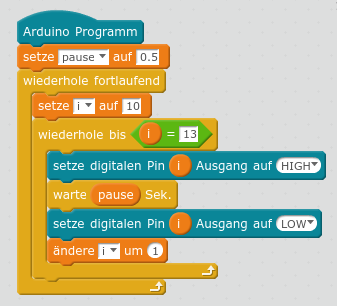
\includegraphics[width=0.9\textwidth]{./lsg/4-2-A1-Lauflicht-Lsg2.png}
		\caption{Programm A.}
	\end{minipage}
	\hfill
	\begin{minipage}{0.52\textwidth}
		\centering
		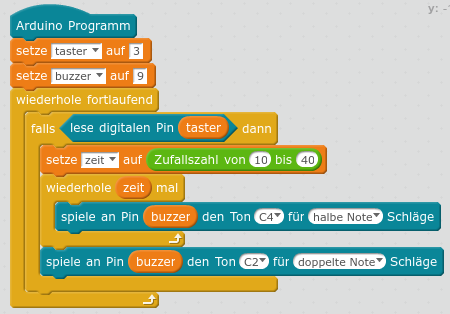
\includegraphics[width=\textwidth]{./lsg/4-3-Bombe-Lsg1.png}
		\caption{Programm B.}
	\end{minipage}
\end{figure}

\newpage

\begin{zsfg}{Darstellung von Programmen in Struktogrammen}
	
	\begin{table}[H]
   \centering
   \begin{minipage}[b]{\textwidth}
      \begin{tabu} to \textwidth {X[L,3]X[L,2]}
         \toprule
         \vspace{-4\baselineskip}
         \textbf{Lineare Struktur}
         
         Jede Anweisung wird in einen rechteckigen Block geschrieben.
          
         &
         \begin{tikzpicture}
         	\draw (0,0) rectangle (5,1);
         	\node at (2.5,0.5) {\footnotesize Anweisung 2};
         	\draw (0,1) rectangle (5,2);
         	\node at (2.5,1.5) {\footnotesize Anweisung 1};
         \end{tikzpicture}
         \\
         \midrule%\hline
         %\rowcolor{CadetBlue!80!green}
         \textbf{Wiederholung / Schleifen} & \\
         \midrule%\hline
%         \vspace{-4.2\baselineskip}
		 \vspace{0mm}
         \textbf{Zählergesteuerte Schleife}
         
         Die Anzahl der Schleifendurchläufe wird durch eine Zählvariable festgelegt. Im Schleifenkopf werden der Startwert der Zählvariablen, der Endwert der Zählvariablen und die Veränderung der Zählvariablen, z.\,B. Schrittweite 1, angegeben.
         &
         \smallbreak
         \vspace{-0.7\baselineskip}
         \begin{tikzpicture}
         	\fill [CadetBlue!70!green] (0,0) rectangle (5,2.2);
         	\draw (0,0) -- (0,2) -- (5,2) -- (5,1) -- (0.2,1) -- (0.2,0) -- (0,0);
         	\draw (0.2,0) -- (5,0) -- (5,1);
         	\node at (2.5,0.5) {\footnotesize Anweisung 1};
         	\node at (2.5,1.5) {\parbox{4cm}{\scriptsize zähle Variable von Startwert bis Endwert, Schrittweite}};
         \end{tikzpicture}
         \\
         \midrule
         \vspace{-4\baselineskip}
         \textbf{Kopfgesteuerte Schleife}
         
         Wiederholungsschleife mit vorausgehender Prüfung der Bedingung. Der Schleifenkörper wird so lange wiederholt, \emph{wie} oder \emph{bis} die Bedingung wahr ist (bei uns nur der letzte Fall verfügbar).
         &
         \begin{tikzpicture}
         \draw (0,0) -- (0,2) -- (5,2) -- (5,1) -- (0.2,1) -- (0.2,0) -- (0,0);
         \draw (0.2,0) -- (5,0) -- (5,1);
         \node at (2.5,0.5) {\footnotesize Anweisung 1};
         \node at (2.5,1.5) {\footnotesize solange, wie/bis Bedingung wahr};
         \end{tikzpicture}
         \\
         \midrule
         \vspace{-4\baselineskip}
         \textbf{Fußgesteuerte Schleife}
         
         Wiederholungsschleife mit nachfolgender Prüfung der Bedingung. Der Schleifenkörper wird so lange wiederholt, \emph{wie} oder \emph{bis} die Bedingung wahr ist (in mBlock nicht verfügbar).\smallskip
         &
         \begin{tikzpicture}
         \draw (0,0) -- (0,2) -- (0.2,2) -- (0.2,1) -- (5,1) -- (5,0) -- (0,0);
         \draw (0.2,2) -- (5,2) -- (5,1);
         \node at (2.5,1.5) {\footnotesize Anweisung 1};
         \node at (2.5,0.5) {\footnotesize solange, wie/bis Bedingung wahr};
         \end{tikzpicture}
         \\
         \midrule%\hline
         %\rowcolor{CadetBlue!80!green}
         \textbf{Verzweigung} & \\
         \midrule%\hline
         \vspace{0mm}
         \textbf{Einfache Verzweigung}
         
         Die Anweisung 1 (und ggf. weitere) wird nur ausgeführt, falls die Bedingung wahr ist. Andernfalls wird nichts gemacht.
         &
         \smallbreak
         \vspace{-0.7\baselineskip}
         \begin{tikzpicture}[scale=0.7]
         \fill [CadetBlue!70!green] (0,0) rectangle (8,2.7);
         \draw (0,0) rectangle (8,2.5);
         \draw (0,1) -- (8,1);
         \draw (4,0) -- (4,1) -- (8,2.5);
         \draw (4,1) -- (0,2.5);
         \node at (2,0.5) {\footnotesize Anweisung 1};
         \node at (1,1.5) {\footnotesize ja};
         \node at (7,1.5) {\footnotesize nein};
         \node at (4,2) {\footnotesize Bedingung};
         \end{tikzpicture}
         \\
         \midrule
         \vspace{-3.5\baselineskip}
         \textbf{Alternative Verzweigung}
         
         Falls die Bedingung wahr ist, wird Anweisung 1 (und ggf. weitere) ausgeführt, sonst wird Anweisung 2 (und ggf. weitere) ausgeführt.
         &
         \begin{tikzpicture}[scale=0.7]
         \draw (0,0) rectangle (8,2.5);
         \draw (0,1) -- (8,1);
         \draw (4,0) -- (4,1) -- (8,2.5);
         \draw (4,1) -- (0,2.5);
         \node at (2,0.5) {\footnotesize Anweisung 1};
         \node at (6,0.5) {\footnotesize Anweisung 2};
         \node at (1,1.5) {\footnotesize ja};
         \node at (7,1.5) {\footnotesize nein};
         \node at (4,2) {\footnotesize Bedingung};
         \end{tikzpicture}
         \\
         \midrule
         \vspace{-5.5\baselineskip}
         \textbf{Verschachtelte Verzweigung}
         
         Falls Bedingung 1 wahr ist, folgt eine weitere Bedingung 2.
         &
         \begin{tikzpicture}[scale=0.7]
         \draw (0,-1.5) rectangle (8,2.5);
         \draw (0,1) -- (8,1);
         \draw (5,-1.5) -- (5,1) -- (8,2.5);
         \draw (5,1) -- (0,2.5);
         \draw (2.5,-1.5) -- (2.5,-0.5) -- (5,1);
         \draw (0,1) -- (2.5,-0.5);
         \draw (0,-0.5) -- (5,-0.5);
         \node at (1,1.5) {\footnotesize ja};
         \node at (7,1.5) {\footnotesize nein};
         \node at (4,2) {\footnotesize Bedingung1};
         \node at (1,0) {\footnotesize ja};
         \node at (4,0) {\footnotesize nein};
         \node at (2.5,0.5) {\footnotesize Bedingung 2};
         \node at (1.25,-1) {\footnotesize Anweisung 1};
         \node at (3.75,-1) {\footnotesize Anweisung 2};
         \node at (6.5,0.5) {\footnotesize Anweisung 3};
         \end{tikzpicture}
         \\
         \bottomrule
      \end{tabu}
   \end{minipage}
	\caption{Tabelle zur Darstellung eines Programms als Struktogramm nach Nassi und Shneidermann.}
   \label{tab:struktogramm}
\end{table}

\end{zsfg}

\section{Vermischte Übungen}

\begin{aufgabe} \emph{Variablen}
	\begin{enumerate}[label=\alph*),itemsep=0mm, parsep=0mm]
		\item Nenne Vorteile, die für die Verwendung von Variablen sprechen.
		\item Nenne drei Datentypen, die in Variablen abgespeichert werden können.
	\end{enumerate}
\end{aufgabe}

\begin{aufgabe} \emph{Schleifen}
	\medskip
	
	\begin{minipage}{0.6\textwidth}
		An allen Digitalpins des Arduino werden LEDs mit geeigneten Vorwiderständen angeschlossen. Dann wird das rechts abgebildete Programm ausgeführt.
		\begin{enumerate}[label=\alph*),itemsep=0mm, parsep=0mm]
			\item Erstelle eine Trace-Tabelle für einen Durchlauf der \button{Wiederhole fortlaufend}- Schleife.
			\item Nenne die Pin-Nummern der LEDs, die nach Durchlaufen dieses Programms einmal geleuchtet haben.
			\item Stelle das Programm als Struktogramm dar.
		\end{enumerate}
	\end{minipage}
	\hfill
	\begin{minipage}{0.38\textwidth}
		\centering
		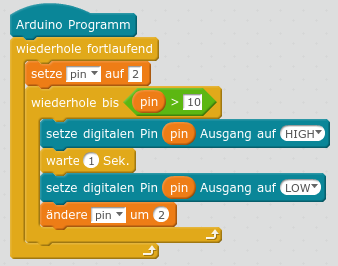
\includegraphics[width=\textwidth]{./pics/programm-trace-uebung.png}
	\end{minipage}
\end{aufgabe}

\bigskip
\begin{aufgabe} \emph{Bitübertragung}
	
	Ein Programm ist 30 kB groß. Berechne, wie lange es bei einer Bitrate von 115200 Bit pro Sekunde dauert, das Programm auf den Arduino zu übertragen.
\end{aufgabe}

\bigskip
\begin{aufgabe} \emph{Das Binärsystem und das Dezimalsystem}
	
	\begin{enumerate}[label=\alph*),itemsep=0mm, parsep=0mm]
		\item Übersetze vom Binär- ins Dezimalsystem.
		\begin{multicols}{3}
			\begin{enumerate}[label=(\arabic*)]
				\item $1001_2$
				\item $1010_2$
				\item $1111_2$
			\end{enumerate}
		\end{multicols}
		\item Übersetze vom Dezimal- ins Binärsystem.
		\begin{multicols}{3}
			\begin{enumerate}[label=(\arabic*)]
				\item 11
				\item 7
				\item 14
			\end{enumerate}
		\end{multicols}
	\end{enumerate}
\end{aufgabe}

\begin{aufgabe} \emph{Programme verstehen}
	
	\begin{minipage}{0.54\textwidth}
		Am Arduino wird an Pin 9 eine LED mit Vorwiderstand und an Pin 10 ein Piezo-Summer angebracht.
		\begin{enumerate}[label=\alph*),itemsep=0mm, parsep=0mm]
			\item Stelle das Programm als Struktogramm dar.
			\item Beschreibe die Wirkung des rechts abgebildeten Programms.
			\item Erkläre, wie man das Programm ändern müsste, damit die LED zwei Mal blinkt, bevor wieder der Piezo-Summer piept.
		\end{enumerate}
		\vspace{2\baselineskip}
	\end{minipage}
	\hfill
	\begin{minipage}{0.45\textwidth}
		\centering
		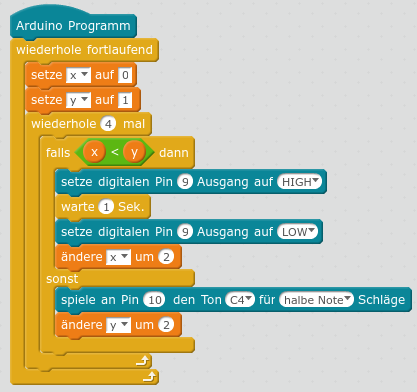
\includegraphics[width=\textwidth]{./pics/Uebung-Variablen-und-Schleifen.png}
	\end{minipage}
\end{aufgabe}

\begin{aufgabe} \emph{Programm entwickeln}
	
	An allen Digitalpins des Arduino sind LEDs mit Vorwiderstand angeschlossen.	Für das folgende Programm ist bereits eine Variable namens \button{p} angelegt. 
	
	Entwickle ein Programm, das die LEDs an Pin 1 bis 5 [2,4,6,8] nacheinander zum Leuchten bringt und nach einer Sekunde wieder ausschaltet. Es leuchtet also immer nur eine LED zur selben Zeit. 
	
	\medskip
	\emph{Anforderungen:}
	\begin{itemize}[noitemsep]
		\item Das Programm soll als Struktogramm dargestellt werden.
		\item Es sollen so wenig Code-Wiederholungen wie möglich vorkommen (\emph{effizientes Programmieren}).
	\end{itemize}
		
	\emph{Befehle:}
	\begin{figure}[H]
		\centering
		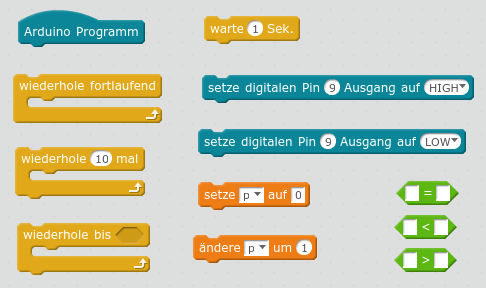
\includegraphics[width=0.6\textwidth]{./pics/Uebung-Programm-entwickeln-Befehlssammlung.png}
	\end{figure}
\end{aufgabe}

\vfill
\begin{links}
	\item \href{https://www.heise.de/make/meldung/Schueler-Projekt-Selbstbau-Staubsaugerroboter-aus-dem-3D-Drucker-3991208.html}{Staubsaugerroboter}
	
	Mithilfe eines Arduino haben zwei Schüler aus den Niederlanden ihren eigenen Staubsaugerroboter gebaut. Das Teile für das Gehäuse haben sie mit einem 3D-Drucker gedruckt.
	
	\item \href{https://www.heise.de/make/artikel/Einfacher-Ultraschall-Levitationsapparat-4022505.html}{Levitation}
	
	Durch Levitation lassen sich Gegenstände scheinbar von Geisterhand in der Luft schweben. Die nötige Elektronik dafür lässt sich mit einem Arduino realisieren.
	
	\item \href{https://www.instructables.com/id/Party-Lights-1/}{Arduino-kontrollierter LED-Streifen zur Visualisierung von Musik}
	
	Der Arduino lässt sich zudem über ein Smartphone ansteuern.
	
	\item \href{https://www.heise.de/make/meldung/Makerbuino-Spielkonsole-fuer-den-Eigenbau-3681578.html}{Spielekonsole von Makerbuino}
	
	Mithilfe eines Bausatzes lässt sich eine kleine, Arduino-basierte Spielekonsole bauen.
\end{links}



\chapter{Analoge Ausgänge und Eingänge}
% analogWrite: Fading von LEDs (Kerzenfunkeln mit drei gelben LEDs), dann Exkurs zur RGB Tabelle und RGB-LED revisited: fast beliebige Farben erzeugen
% Potentiometer und dimmbare Lampe; Exkurs: Nutzung des Potentiometers ohne Mikrocontroller
Digitale Bauteile haben ein Problem: Sie kennen nur Eins oder Null, An oder Aus, Wahr oder Falsch. Die Realität ist aber natürlich um einiges komplexer, nämlich analog: Reale Größen können durch im Prinzip beliebige reelle Zahlen ausgedrückt werden. Daher wäre es wünschenswert, auch analoge Werte angeben zu können. In diesem Kapitel lernst du, wie man mit dem Arduino quasi-analoge Werte erzeugen oder einlesen kann. Dabei ist es nie möglich, wirklich beliebig genaue Werte zu erreichen, wie man es bei analogen Werten erwarten würde, aber es gibt einige interessante Tricks, wie man mit einem digitalen Bauteil analoge Werte simulieren kann.

\bigskip
In diesem Kapitel lernst du\dots
\begin{itemize}
	\item \dots Pulsweitenmodulation und Hexadezimalzahlen zu benutzen,
	\item \dots Spannungen zu messen und Spannungen an einem Spannungsteiler zu berechnen,
	\item \dots logische Bedingungen mit logischen Operationen zu verfeinern,
	\item \dots ein Potentiometer, einen LDR sowie einen NTC auszulesen, um eine Drehung, die Umgebungshelligkeit bzw. die Temperatur zu messen,
	\item \dots wie Transistoren verwendet werden und was diese mit dem Aufbau des Arduino zu tun haben,
	\item \dots was es mit dem EVA-Prinzip auf sich hat.
\end{itemize}

\bigskip

\begin{projektueberblick}
	\item Kerzenfunkeln \dotfill \pageref{proj:kerzen}
	\item Farbenspektakel mit RGB-Codes \dotfill \pageref{proj:rgbled2}
	\item Batterietester (kleine Spannung) \dotfill \pageref{proj:batterietesterklein}
	\item Batterietester (große Spannung) \dotfill \pageref{proj:batterietestergross}
	\item Dimmbare Lampe \dotfill \pageref{proj:dimmlampe}
	\item Dimmbare Lampe ohne $\mu C$ \dotfill \pageref{proj:dimmlampeomc}
	\item Straßenlampe \dotfill \pageref{proj:strassenlampe}
	\item Alarmanlage \dotfill \pageref{proj:alarmanlage}
	\item Thermometer \dotfill \pageref{proj:thermometer}
\end{projektueberblick}
\newpage

\section{Pulsweitenmodulation (PWM)}\label{sec:pwm}

\begin{ziel}
	\textbf{Ziel:} Mithilfe des Arduino soll eine funkelnde LED-Kerze gebaut werden.
\end{ziel}

\begin{wrapfigure}{r}{0.35\textwidth}
	\centering
	
\includegraphics[width=0.35\textwidth]{./pics/analogwrite.png}
\end{wrapfigure}
Der Arduino verfügt über mehrere sogenannte PWM-Pins, die mit einer Tilde ($\sim$) gekennzeichnet sind. Diese lassen sich mit dem Befehl \button{setze PWM-Pin <\_> Ausgang auf <\_>} ansteuern. Im ersten Argument muss die Nummer des Pins angegeben werden, im zweiten Argument wird ein PWM-Wert zwischen 0 und 255 angegeben.

\begin{aufgabe} \emph{Fading}
	\begin{enumerate}[label=\alph*), itemsep=0ex, parsep=0ex]
		\item Schließe eine LED mit Vorwiderstand an einen PWM-Pin an und verwende die PWM-Anweisung mit unterschiedlichen PWM-Werten. Beschreibe die Wirkung auf die LED in einem Je-Desto-Satz.
		\item Lege eine Variable \button{h} für den PWM-Wert an. Nutze die Variable, um systematisch alle PWM-Werte von 0 bis 255 zu durchlaufen, sodass jeder Wert kurz sichtbar wird (z.\,B. 0.2 Sekunden).
		\item \emph{Für Schnelle:} Sorge dafür, dass die PWM-Werte nach Erreichen der 255 genauso rückwärts von 255 bis 0 durchlaufen werden.
	\end{enumerate}
\end{aufgabe}

\begin{aufgabe} \emph{Pulsweitenmodulation}
	
	Erkläre mithilfe der Zusammenfassung zur Pulsweitenmodulation, was bei der Nutzung des Befehls \button{Setze PWM-Pin 5 Ausgang auf 158} passiert. Berechne auch die mittlere Spannung, die am PWM-Pin ausgegeben wird.
	
	\emph{Für Physik-Profis:} Eine blaue LED hält bis zu 3,5\,V aus, ohne durchzubrennen. Trotzdem darf man sie bei Verwendung dieses Befehls nicht ohne Vorwiderstand an den Pin anschließen. Begründe.
	
	\emph{Für Informatik-Profis:} Wie viel Bit stehen zur Speicherung des Tastverhältnisses mit Werten von 0 bis 255 zur Verfügung?
\end{aufgabe}

\marginpar{%
	\footnotesize%
	\werkzeug Neues \\
	Werkzeug:\\
	\hyperref[sec:servo]{Servo-\\motor}%
}
\begin{projekt}[Kerzenfunkeln]\label{proj:kerzen}
	Modelliere mithilfe von drei LEDs das Funkeln von Kerzen.
	
	Tipp: Die Verwendung des Blocks für Zufallszahlen wird dir helfen, das Funkeln natürlicher aussehen zu lassen.
\end{projekt}

\newpage

\begin{zsfg}{Pulsweitenmodulation (PWM)}
	
	\begin{wrapfigure}{r}{0.45\textwidth}
		\centering
		\begin{tikzpicture}[scale=0.8]
		\fill [white] (-1.2,-1.3) rectangle (7,7.1);
		\draw [->] (0,-1) -- (0,6.5);
		\draw [->] (-1,0) -- (6.5,0);
		\draw [dashed] (4,-1) -- ++(0,7.5);
		\node at (-0.2,-0.3) {\scriptsize 0};
		\foreach \x in {1,...,6} {
			\draw (\x,0.1) -- (\x,-0.1) node [anchor=north, fill=white] {\scriptsize\x};
			\draw (0.1,\x) -- (-0.1,\x) node [anchor=east] {\scriptsize\x};
		}
		\node at (6.5,-0.35) {\scriptsize Zeit};
		\node at (0,6.5) {\parbox{1.7cm}{\scriptsize El. Potential in V}};
		\draw [thick, blue] (0,5) -- ++(1,0) ++(0,-5) -- ++(3,0) ++(0,5) -- ++(1,0) ++(0,-5) -- ++(1.5,0);
		\draw [thick, red] (0,1.25) -- ++(6.5,0) node [above] {$\overline{U}$};
		\draw [<->] (0,-0.6) -- (4,-0.6) node [below left=1mm] {\scriptsize Periodendauer T};
		\end{tikzpicture}
		\caption{Darstellung des zeitlichen Verlaufs einer Pulsweitenmodulation mit einem Tastverhältnis von 25\%.}
	\end{wrapfigure}
	Bei der Pulsweitenmodulation wechselt der ausgewählte digitale Pin sehr schnell zwischen den elektrischen Potentialen 5\,V und 0\,V hin und her - es ergibt sich also ein gepulstes Signal, dessen Weite (Dauer) moduliert werden kann. Aus dem Verhältnis der Zeit, in der der Pin auf einem 5\,V-Potential liegt, zu der Zeit, in der der Pin auf einem 0\,V-Potential liegt, ergibt sich eine mittlere Spannung (gegenüber Ground), die scheinbar am Pin anliegt. Wenn der Pin in der Hälfte der Zeit auf 5\,V und in der anderen Hälfte auf 0\,V liegt, dann ergibt sich eine mittlere Spannung von $\overline{U}=2,5\,V$. Wenn der Pin nur in einem Viertel der Zeit auf 5\,V liegt, dann ergibt sich eine mittlere Spannung von $\overline{U}=1,25\,V$ ($=5\,V\cdot 0,25$).
	
	Das Verhältnis der Zeit mit 5\,V zu der Gesamtdauer einer Periode mit 5\,V und 0\,V wird als \emph{Tastverhältnis} bezeichnet. Im Programm wird das Tastverhältnis durch einen Wert zwischen 0 und 255 angegeben. Eine 0 bedeutet, dass die Zeit mit 5\,V 0\% ausmacht, also liegt der Pin durchgängig auf einem 0\,V-Potential. Eine 255 bedeutet, dass die Zeit mit 5\,V 100\% ausmacht, also liegt der Pin durchgängig auf einem 5\,V-Potential. Diese beiden Werte entsprechen dem, was bei den bekannten Befehlen zur Steuerung von digitalen Pins passiert.
	
	Ein Wert von 100 bedeutet einen Anteil von $\frac{100}{255}\approx 0,39$ der Periodendauer. Daraus ergibt sich eine mittlere Spannung von $\overline{U}=5\,V\cdot 0,39\approx 1,96\,V$.
\end{zsfg}

\newpage
\subsection{RGB-Farben aus Hexadezimalzahlen erzeugen}\label{proj:rgbled2}

Als wir uns das erste Mal die RGB-LED angeschaut haben (siehe S. \pageref{proj:rgbled1}), war die Anzahl der Farben, die wir erzeugen konnten, noch stark limitiert. Das ändert sich mit der Möglichkeit, die Farbanteile über PWM zu dimmen. Häufig werden die Farbanteile im RGB-Modell jedoch nicht in Dezimalzahlen zwischen 0 und 255 angegeben, sondern durch Hexadezimalzahlen - z.\,B. \texttt{\#CAFF70}.

\begin{ziel}
	\textbf{Frage:} Wie kann man aus dem RGB-Hexadezimal-Code die PWM-Werte bestimmen?
\end{ziel}

\begin{aufgabe} \emph{Hexadezimalzahlen}
	\begin{enumerate}[label=\alph*), itemsep=0ex, parsep=0ex]
		\item Du kennst bereits das Dezimalsystem zur Basis 10 mit Ziffern von 0 bis 9 und das Binärsystem zur Basis 2 mit den Ziffern 0 und 1. Der RGB-Code nutzt eine Raute zu Anfang und danach das Hexadezimalsystem zur Basis 16. Wie viele Ziffern gibt es hier? Stelle anhand des Beispielcodes \texttt{\#CAFF70} eine Vermutung darüber auf, wie die Ziffern lauten.
		\item Der RGB-Code lässt sich in drei Zahlen zerlegen, die die Anteile von Rot, Grün und Blau angeben:
		\begin{equation*}
			 \# \underbrace{\texttt{CA}}_{\text{Anteil Rot~}} \underbrace{\texttt{FF}}_{\text{Anteil Grün~}} \underbrace{\texttt{70}}_{\text{Anteil Blau}}.
		\end{equation*}
		Rechne die einzelnen Zahlen vom Hexadezimalsystem ins Dezimalsystem um.
		
		\emph{Zur Erinnerung:} Im Dezimalsystem bedeutet die Zahl $70$: $7\cdot 10^1 + 0 \cdot 10^0$. Übertrage diese Zerlegung für das Hexadezimalsystem. Übersetze die Buchstabenziffern vorher ins Dezimalsystem ($\texttt{A}_{16}=10_{10},~ \texttt{B}_{16}=11_{10}, \dots$).
		\item \emph{Für Denker:} Wie viele verschiedene Farben kann man mithilfe des RGB-Farbcodes darstellen?
	\end{enumerate}
\end{aufgabe}

\begin{aufgabe} \emph{RGB-Codes}
	\begin{enumerate}[label=\alph*), itemsep=0ex, parsep=0ex]
		\item Bestimme anhand des RGB-Hexadezimal-Farbcodes die PWM-Werte für Rot, Grün und Blau in der folgenden Tabelle.
		\item Schließe eine RGB-LED mit Vorwiderstand an den Arduino an (siehe S. \pageref{proj:rgbled1}) und erzeuge nacheinander die Farben aus der Tabelle.
	\end{enumerate}
\end{aufgabe}

% die Farben für diese Tabelle sind in commands.tex mithilfe des xcolor-Pakets definiert
\begin{table}[H]
	\centering
	\begin{minipage}[c]{\textwidth}
		\begin{tabu} to \textwidth {X[L,2]X[L]X[L]|X[L,2]X[L]X[L]}
			\toprule
			\textbf{Farbe} & \textbf{Hex-Code} & \textbf{PWM-Werte} & \textbf{Farbe} & \textbf{Hex-Code} & \textbf{PWM-Werte} \\
			\midrule
			\textcolor{blueviolet}{\rule{1cm}{0.4cm}} Blue-Violet	& \texttt{\# 8A2BE2} &  & \textcolor{olivedrab}{\rule{1cm}{0.4cm}} OliveDrab & \texttt{\# 6B8E23} &  \\ 
			\textcolor{turquoise1}{\rule{1cm}{0.4cm}} Turquoise1	& \texttt{\# 00F5FF} &  & \textcolor{khaki}{\rule{1cm}{0.4cm}} Khaki & \texttt{\# F0E68C} &  \\
			\textcolor{chocolate}{\rule{1cm}{0.4cm}} Chocolate	& \texttt{\# D2691E} &  & \textcolor{deeppink}{\rule{1cm}{0.4cm}} DeepPink & \texttt{\# FF1493} &  \\
			\bottomrule
		\end{tabu}
	\end{minipage}
	\label{tab:rgb-codes}
\end{table}

\begin{projekt}[Farbenspektakel mit RGB-Farbcodes]
	Lasse die RGB-LED mithilfe des Fadings (vgl. Aufgabe \emph{Fading} zur PWM) möglichst viele Farbwerte durchlaufen und beobachte das Funkeln.
\end{projekt}
\newpage
\newgeometry{twoside, top=1cm, outer=2.6cm, inner=2.6cm, % inner und outer sind aus irgendeinem Grund vertauscht
	marginparwidth=2cm, marginparsep=0.3cm,% Die Breite für die Marginalien (Randbemerkungen) auf der rechten Seite
	bottom=1cm, footskip=24pt, %Abstand zwischen Textboden und Fußzeilenboden
	includefoot, includehead}
\begin{zsfg}{Das Hexadezimalsystem}
	
	Im Gegensatz zum Dezimalsystem zur Basis 10 mit Ziffern von 0 bis 9 und zum Binärsystem zur Basis 2 mit den Ziffern 0 und 1 arbeitet das Hexadezimalsystem mit der Basis 16 und den Ziffern 0, \dots, 9, A, B, C, D, E, F. Die Buchstaben werden als Ziffern gewählt, weil bei der üblichen 10, 11, 12, ... nicht deutlich würde, dass es sich nur um \emph{eine} Ziffer zur Basis 16 handelt.
	
	Im Hexadezimalsystem wird jede Zahl durch die Potenzen von 16 zusammengesetzt. Die Hexadezimalzahl \texttt{AF5} bedeutet dann so viel wie $\texttt{A}\cdot 16^2 + \texttt{F}\cdot 16^1 + \texttt{5}\cdot 16^0$. Den Wert der Hexadezimalzahl im Dezimalsystem erhält man dann durch eben diese Rechnung, wobei für die Buchstabenziffern die Dezimalzahlen eingesetzt werden müssen: $10\cdot 16^2 + 15\cdot 16 + 5\cdot 1 = 2805$.
	
	Da bei kleineren Ziffern wie \texttt{405} nicht ersichtlich ist, ob es sich um eine Hexadezimalzahl handeln soll, wird der Zahl häufig ein \texttt{0x} vorangestellt: \texttt{0x405}. Ebenfalls üblich ist es, die Basis im Index zu notieren: $\texttt{405}_{16}$ zeigt eine Hex-Zahl an; $405_{10}$ eine Dezimalzahl.
	
	\bigskip
	\textbf{Der RGB-Farbcode}
	
	Der RGB-Farbcode setzt jede Farbe aus Rot, Grün und Blau zusammen, wobei jede Farbe einen unterschiedlichen Anteil an der Mischung haben kann. Der Anteil wird durch eine Zahl zwischen 0 und 255 ausgedrückt; es steht für jede Farbe also ein Byte (acht Bit) zur Verfügung.
	
	Es wäre allerdings umständlich und für Menschen schlecht lesbar, für jede Farbe acht Nullen bzw. Einsen zu notieren. Die entsprechenden Dezimalzahlen wären zwar schon übersichtlicher, jedoch lassen sich Dezimalzahlen von digitalen Bauteilen schlechter verarbeiten, weil die 10 keine Zweierpotenz ist. Die Basis 16 schafft hier Abhilfe: Als vierte Potenz von Zwei ($16=2^4$) lassen sich die Ziffern zur Basis 16 durch genau vier Bit darstellen. Zum Beispiel ist $13_{10}=\texttt{D}_{16}=1101_2$. Zweistellige Hex-Zahlen lassen sich dann durch acht Bit, also ein Byte darstellen. Der Wertebereich reicht von \texttt{00} (also 0) bis \texttt{FF} (also $15\cdot 16 + 15 \cdot 1=255$) und passt damit genau zum RGB-Farbraum.
	
	\begin{wrapfigure}{r}{0.45\textwidth}
		\centering
		%\vspace{-1.5\baselineskip}
		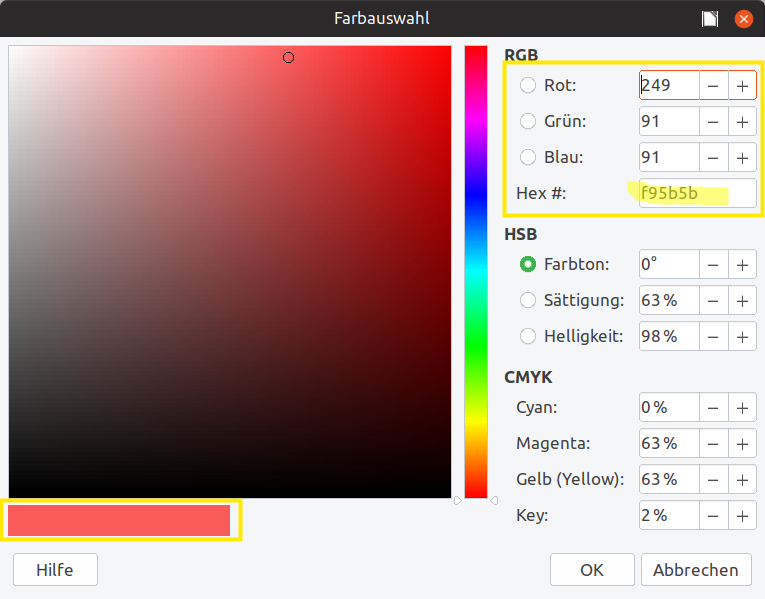
\includegraphics[width=0.45\textwidth]{./pics/Farbauswahl-LibreOffice.png}
		\caption{RGB-Farbcode in LibreOffice (rechts oben; die Angabe erfolgt über Dezimalzahlen oder Hexzahlen).}
		%\vspace{-1\baselineskip}
	\end{wrapfigure}
	Um deutlich zu machen, dass die folgenden Hex-Zahlen eine Farbe im RGB-Code codieren, wird den drei Hex-Zahlen für die drei Farbanteile eine Raute vorangestellt. Aus den insgesamt sechs Ziffern, für die jeweils 16 mögliche Werte existieren, ergeben sich $16^6=16777216$ verschiedene Farben, die sich codieren lassen. Das sind mehr Farben als das menschliche Auge unterscheiden kann.
	
	RGB-Farbcodes werden in zahlreichen Programmen wie zum Beispiel der Textverarbeitung LibreOffice genutzt (siehe Abbildung rechts). Im Internet findet man zudem \href{http://www.farb-tabelle.de/de/farbtabelle.htm}{Farbtabellen mit der Angabe der Codes}.
\end{zsfg}
\restoregeometry
\onehalfspacing

\section{Spannung messen an analogen Eingängen}

Wenn Batterien kaum noch Ladung gespeichert haben, lässt die Spannung an ihren Polen nach und sinkt unter den Wert, der auf der Batterie vermerkt ist. Mithilfe der analogen Eingänge A0 bis A5 lässt sich die Spannung messen und so entscheiden, ob die Batterie noch brauchbar ist.
\marginpar{%
	\textattachfile[description={Arbeitsblatt zu Kap. \thechapter, Spannung messen}]{./Auftraege/kap5-batterietester.pdf}{
	\footnotesize%
	\drucker Vorlage%
	}%
	\footnotesize%
	%\drucker \href{run:./Auftraege/kap5-batterietester.pdf}{Vorlage}
	\\öffnen%
}

\begin{ziel}
	\textbf{Frage:} Wie kann man mit dem Arduino eine Spannung messen?
\end{ziel}

\marginpar{%
	\scriptsize%
	\ausrufezeichen Achtung: \\
	Ganze Zahlen:\\
	10/1023 \\
	= 0 \\
	Kommazahlen:\\
	10/1023.0 \\
	= 0.01
}
\begin{projekt}[Batterietester (Voltmeter für $U<5\,V$)]\label{proj:batterietesterklein}
	\begin{wrapfigure}{r}{0.3\textwidth}
		\centering
		\begin{tabular}{c | c}
			\textbf{Analogwert} & \textbf{Spannung} \\ \hline
			0 & 0\,V \\ \hline
			1 &  \\ \hline
			100 &  \\ \hline
			1023 & 5\,V \\ \hline
		\end{tabular}
	\end{wrapfigure}
	Für eine einfache Messung bei einer 1,5\,V-Batterie wird der negative Pol der Batterie mit GND verbunden, sodass ein gemeinsames Nullpotential vorliegt. Der positive Pol der Batterie wird mit einem der analogen Eingänge A0 bis A5 verbunden. Über einen eingebauten Analog-Digital-Wandler (\emph{engl. analog-to-digital converter, ADC}) wird der Spannungswert durch eine Zahl zwischen 0 und 1023 ausgedrückt.
	 
	\begin{enumerate}[label=\alph*), itemsep=0mm, parsep=0mm]
	 	\item Schließe eine mit 1,5\,V beschriftete Batterie an den Arduino an und miss die Spannung. Berechne aus dem Analogwert die Spannung und lass sie auf dem seriellen Monitor ausgeben.
	 	\item Ergänze den Batterietester um eine Ampel, die anzeigt, ob die Batterie voll aufgeladen bzw. noch in Ordnung bzw. leer ist.
	 	\item \emph{Für Informatik-Profis:} Wie viel Bit Speicherplatz werden für den Analogwert zwischen 0 und 1023 gebraucht?
	\end{enumerate}	
\end{projekt}
%\footnotesize Achtung: Das Programm rechnet 100/1023 = 0 (Division ganzer Zahlen mit Abrundung), 100/1023.0 = 0.0978 (Division von Gleitkommazahlen).

%\normalsize

\begin{projekt}[Batterietester (Voltmeter für $U>5\,V$)]\label{proj:batterietestergross}
	Da der Arduino beim direkten Anschließen nur maximal 5\,V \enquote{verträgt}, muss man zum Testen von z.\,B. 9\,V-Blöcken weitere Bauteile verwenden. Mit zwei $\SI{10}{\kilo\ohm}$ Widerständen kann man einen einfachen \emph{Spannungsteiler} aufbauen, der die Messung ermöglicht.
	%\vspace{-\baselineskip}
	\begin{minipage}{\textwidth}
		\begin{minipage}{0.48\textwidth}
			\begin{enumerate}[label=\alph*), itemsep=0mm, parsep=0mm]
				\item Berechne die Stromstärke und die Spannung an den Widerständen. Warum sind große Widerstände hier sinnvoll?
				\item Markiere die Kabel in der Abbildung farbig, sodass die Kabel, die auf dem gleichen elektrischen Potential liegen, die gleiche Farbe haben. Notiere zudem den Wert des elektrischen Potentials.
			\end{enumerate}
		\end{minipage}
		\hfill
		\begin{minipage}{0.48\textwidth}
			\centering
			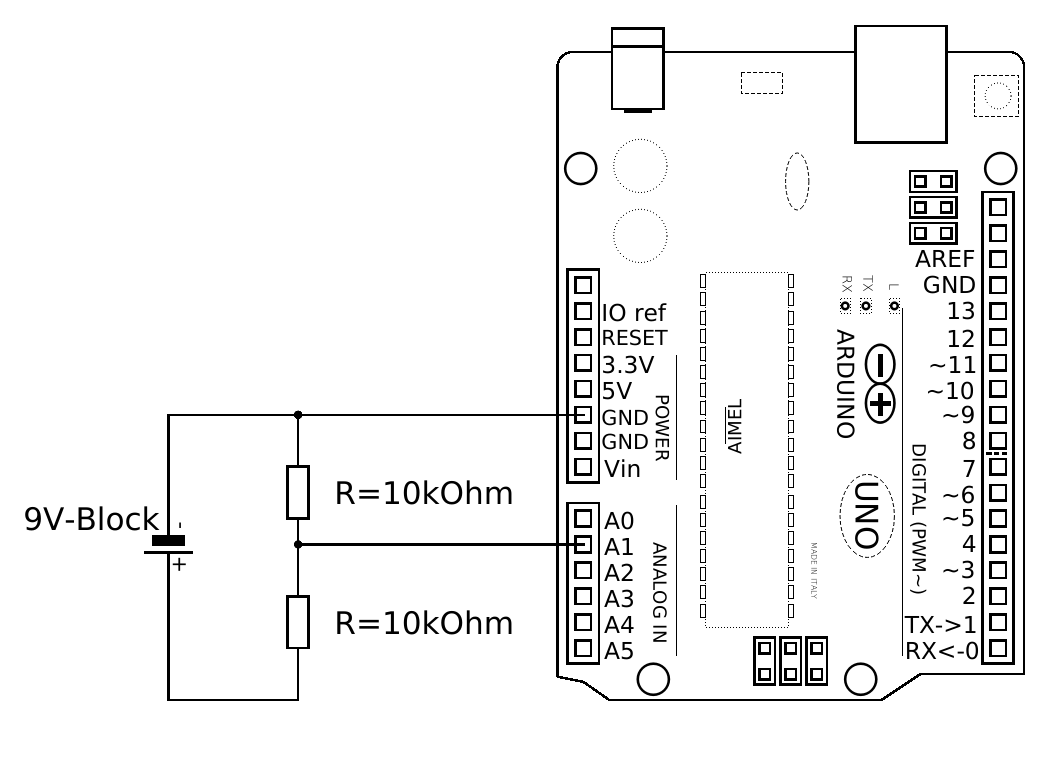
\includegraphics[width=0.95\textwidth]{./Zeichnungen/schaltplan-batterietester.png}
		\end{minipage}
	\end{minipage}
	\begin{enumerate}[label=\alph*), itemsep=0mm, parsep=0mm,start=3]
		\item Gib an, wie man mit dem Arduino die Spannung am 9\,V-Block berechnet. Baue den Batterietester dann auf und probiere ihn mit dem 9\,V-Block aus der Box aus.
		\item \emph{Zum Nachdenken:} Wie groß darf die Spannung beim oben verwendeten Spannungsteiler maximal sein, damit am Arduino nicht mehr als 5\,V anliegen? Wie könnte man den Spannungsteiler bauen, sodass man Spannungen bis zu 15\,V messen kann?
	\end{enumerate}
\end{projekt}

% Hinweis: Ganz ähnlich funktioniert ein Multimeter, bei dem man verschiedene Bereiche zum Messen der Spannung einstellen kann! Auch dort werden die Messwiderstände möglichst groß gehalten, um den Strom durch das Messgerät möglichst klein zu halten.
% Zusammenfassung: Spannung messen am Arduino und Spannungsteiler?!

\subsection{Bedingungen durch logische Operationen verfeinern}
% Beim Bau der Batterieampel kann man die und Verknüpfung verwenden -> Aufhänger zum Betrachten von kombinierten Wahrheitswerten
\marginpar{%
	\textattachfile[description={Folie zu Kap. \thechapter, Logische Operationen}]{./Auftraege/kap5-batterieampel-wahrheitswerte.pdf}{%
		\folie\footnotesize Folie%
	}%
	\footnotesize%
	%\folie \href{run:./Auftraege/kap5-batterieampel-wahrheitswerte.pdf}{Folie} \\
	\\öffnen
}
Beim Bau der Batterieampel kann die Verknüpfung von Wahrheitswerten hilfreich sein. Dazu dienen die Blöcke für die logischen Operationen \button{und}, \button{oder} und \button{nicht}, die aus zwei Bedingungen, die jeweils wahr oder falsch sein können, einen zusammenfassenden Wahrheitswert (wahr/falsch) machen bzw. den Wahrheitswert umkehren (\enquote{NICHT}).

\begin{ziel}
	\textbf{Frage:} Wie ermittelt man das Ergebnis der logischen Operationen NICHT, UND, ODER?
\end{ziel}

\begin{aufgabe} \emph{Genau draufgeschaut: Batterieampel}
	
	Wenn man die Batterieampel mit logischen Operationen realisiert, braucht man eine Bedingung der folgenden Art:
	\begin{equation*}
		spannung > 1,2\,V \quad \text{UND} \quad  spannung < 1,4\,V \quad  \text{ODER} \quad spannung = 1,4\,V
	\end{equation*}
	
	Dies lässt sich bei mBlock auf zwei Arten realisieren, die sich in der Reihenfolge der Auswertung unterscheiden (siehe Abbildung).
	
	\begin{figure}[H]
		\centering
		\includegraphics[width=0.6\textwidth]{./pics/batterieampel-log-operationen.png}
	\end{figure}

	Sind beide Varianten geeignet?
	
	Zur Klärung dieser Frage eignen sich in einfachen Fällen \textbf{Wahrheitswerttabellen}, die einen Überblick über das Ergebnis der logischen Operationen bieten (siehe unten). Vergleiche die beiden Varianten mithilfe von Wahrheitswerttabellen.
	
	\bigskip
	\textbf{Variante 1:}
	
	\medskip
	\begin{minipage}{\textwidth}
		\small
		\centering
		\begin{tabular}{c|c|c|c|c|c}
			U>1,2\,V & U<1,4\,V & U=1,4\,V & U<1,4\,V ODER U=1,4\,V & \parbox{4cm}{U>1,2\,V UND (U<1,4\,V ODER U=1,4\,V)} & Bemerkung\\ \hline
			1 & 1 & 1 & 1 & 1 & phys. unmögl. \\
			0 & 1 & 1 & 1 & \dots & \dots\\
			\dots & \dots & \dots & \dots & \dots & \dots\\
		\end{tabular}
	\end{minipage}
	
	\bigskip
	\textbf{Variante 2:}
	
	\medskip
	\begin{minipage}{\textwidth}
		\small
		\centering
		\begin{tabular}{c|c|c|c|c|c}
			U>1,2\,V & U<1,4\,V & U=1,4\,V & U>1,2\,V UND U<1,4\,V & \parbox{4cm}{(U>1,2\,V UND U<1,4\,V) ODER U=1,4\,V} & Bemerkung\\ \hline
			1 & 1 & 1 & 1 & 1 & phys. unmögl. \\
			0 & 1 & 1 & 0 & \dots & \dots \\
			\dots & \dots & \dots & \dots & \dots & \dots\\
		\end{tabular}
	\end{minipage}
\end{aufgabe}

\begin{minipage}{0.75\textwidth}
	\begin{aufgabe} \emph{Juke-Box 2.0}
			
		Logische Operationen lassen sich nutzen, um die Juke-Box aus Kapitel 2 zu erweitern, ohne Hardware nachrüsten zu müssen. Zur Erinnerung: Es wurden zwei Taster und ein Piezo-Summer an den Arduino angeschlossen. Wenn Taster 1 gedrückt wurde, gibt der Befehl \button{lese digitalen Pin taster1} TRUE zurück und es wurde ein entsprechender Song gespielt.
		
		Die Idee: Man kann auch beide Taster gleichzeitig oder gar keinen Taster drücken, sodass sich vier Fälle für vier Songs ergeben. Sinnvollerweise wird nur irgendeine Standardmusik gespielt, wenn gar kein Taster gedrückt wurde.
		
		Formuliere für jeden der vier Fälle eine trennscharfe Bedingung!
	\end{aufgabe}
\end{minipage}
\hfill
\begin{minipage}{0.23\textwidth}
	\centering
	\includegraphics[width=0.98\textwidth]{./pics/jukebox2-0-leer.png}
\end{minipage}
\marginpar{%
	\textattachfile[description={Arbeitsblatt zu Kap. \thechapter, De Morgan}]{./Auftraege/kap5-wahrheitswerte-de-morgan.pdf}{%
		\ausrufezeichen
	}
	\footnotesize%
	%\ausrufezeichen \href{run:./Auftraege/kap5-wahrheitswerte-de-morgan.pdf}{De Morgan}
	De Morgan
}


\begin{zsfg}{Logische Operationen und Wahrheitswerttabellen}
	
	Logische Operationen dienen zum Verknüpfen von Wahrheitswerten - ganz so wie Rechenoperationen zum Verknüpfen von Zahlen dienen. Wir betrachten die logischen Operationen UND (AND), ODER (OR) sowie NICHT (NOT). Das Ergebnis dieser Operationen lässt sich anhand von Wahrheitswerttabellen übersichtlich festhalten. Darin wird festgehalten, ob zwei Aussagen bzw. Bedingungen A und B wahr (1) oder falsch (0) sind. In der rechten Spalte steht dann, ob die logische Operation wahr (1) oder falsch (0) ergibt.
	
	\medskip
	\begin{minipage}{0.3\textwidth}
		\centering
		\begin{tabular}{c | c | c}
			\textbf{A} & \textbf{B} & \textbf{A UND B} \\ \hline
			1 & 1 & 1 \\
			1 & 0 & 0 \\
			0 & 1 & 0 \\
			0 & 0 & 0 \\  
		\end{tabular}
	\end{minipage}
	\hfill
	\begin{minipage}{0.3\textwidth}
		\centering
		\begin{tabular}{c | c | c}
			\textbf{A} & \textbf{B} & \textbf{A ODER B} \\ \hline
			1 & 1 & 1 \\
			1 & 0 & 1 \\
			0 & 1 & 1 \\
			0 & 0 & 0 \\  
		\end{tabular}
	\end{minipage}
	\hfill
	\begin{minipage}[t]{0.3\textwidth}
		\centering
		\begin{tabular}{c | c}
			\textbf{A}  & \textbf{NICHT A} \\ \hline
			1 & 0 \\
			0 & 1 \\  
		\end{tabular}
	\end{minipage}
	
	\medskip
	Achtung: Die ODER-Operation ergibt auch dann \enquote{wahr}, wenn beide Aussagen wahr sind. Das aus dem Alltag bekannte \enquote{ENTWEDER-ODER} (XOR) ist eine weitere logische Operation, die \enquote{falsch} ergibt, wenn beide Aussagen wahr sind. Diese Operation ist aber nicht in mBlock enthalten.
\end{zsfg}

\newpage
\newgeometry{twoside, top=2cm, outer=2.6cm, inner=2.6cm, % inner und outer sind aus irgendeinem Grund vertauscht
	marginparwidth=2cm, marginparsep=0.3cm,% Die Breite für die Marginalien (Randbemerkungen) auf der rechten Seite
	bottom=1cm, footskip=24pt, %Abstand zwischen Textboden und Fußzeilenboden
	includefoot, includehead}
\section{Die Verwendung eines Potentiometers (Drehreglers)} \label{sec:potentiometer}
% Bleistiftpoti
Die Messung einer variablen, (quasi-)analogen Spannung eröffnet neue Möglichkeiten, da die Eingabewerte nun viel differenzierter sind als bei einem Taster, bei dem die Eingabe nur aus \enquote{0} oder \enquote{1} bestand. Zum Beispiel kann man darüber angeben, wie hell eine Lampe leuchten soll bzw. wie stark sie gedimmt werden soll. Dazu werden Potentiometer verwendet.

\begin{ziel}
	\textbf{Frage:} Wie funktioniert ein Potentiometer?
\end{ziel}
\marginpar{%
	\textattachfile[description={Folie zu Kap. \thechapter, Bleistiftpotentiometer}]{./Auftraege/kap5-bleistiftpoti.pdf}{%
		\footnotesize\folie Folie%
	}
	\footnotesize%
	%\folie \href{run:./Auftraege/kap5-bleistiftpoti.pdf}{Folie} \\
	\\öffnen%
}
\vspace{-1\baselineskip}
\begin{aufgabe}\emph{Bleistiftpotentiometer}
	
	\begin{minipage}{0.6\textwidth}
		\smallskip
		Ein einfaches Potentiometer kannst du selbst bauen. 
		
		\smallskip
		\emph{Basteln:} Markiere dafür mit Bleistift einen dicken Strich auf einem Blatt Papier und klebe am einen Ende ein Kabel fest, das mit GND verbunden ist. Klebe ans andere Ende ein Kabel, das mit 5V verbunden ist. Mit einem dritten Kabel (\enquote{Sensorkabel}), das mit einem analogen Eingang verbunden ist, lässt sich nun messen, welches elektrische Potential an einer beliebigen Stelle des Bleistiftstreifens anliegt.
		
		\smallskip
		\emph{Experimentieren:}	Schreibe ein Programm, dass dir fortlaufend auf dem seriellen Monitor die Analogwerte und die umgerechneten Werte für das elektrische Potenzial bzw. die Spannung gegenüber GND anzeigt. Bewege dann das Sensorkabel über den Streifen und beobachte, wie sich die Spannungswerte verändern.
	\end{minipage}
	\hfill
	\begin{minipage}{0.39\textwidth}
		\centering
		\includegraphics[width=0.75\textwidth]{./pics/bleistiftpoti-klein.png}
	\end{minipage}

	\medskip
	\emph{Analysieren:}	Der Bleistiftstreifen leitet den Strom bei einem bestimmten Gesamtwiderstand $R_{ges}$. Durch das Sensorkabel wird der Streifen in zwei Teile mit den Teilwiderständen $R_1$ und $R_2$ geteilt. Erläutere anhand deiner Beobachtungen, wie die drei Widerstände zusammenhängen.
	
	{\scriptsize Idee: Frick, Fritsch und Trick (2015): \emph{Einführung in Mikrocontroller - Der Arduino als Steuerzentrale}, Bad Saulgau}
\end{aufgabe}

\begin{zsfg}{Potentiometer}
	\begin{minipage}{0.7\textwidth}
		Ein \textbf{Potentiometer}, kurz: Poti, ist im Grunde nichts anderes als ein Spannungsteiler mit zwei Widerständen. Jedoch kann die Größe der Widerstände z.\,B. durch Drehen variiert werden. Der Gesamtwiderstand bleibt dabei immer gleich.
	\end{minipage}
	\hfill
	\begin{minipage}{0.28\textwidth}
		\begin{minipage}{0.48\textwidth}
			\centering
			\includegraphics[angle=-90,width=0.8\textwidth]{./pics/poti.jpg}
		\end{minipage}
		\hfill
		\begin{minipage}{0.48\textwidth}
			\centering
			\includegraphics[width=0.65\textwidth]{./pics/poti-schaltsymbol.png}
		\end{minipage}
	\end{minipage}
	
	\smallskip
	Beim Anschluss an den Arduino wird der mittlere Pin des Potentiometers an einen analogen Eingang angeschlossen. Die anderen beiden Pins werden mit GND und 5V verbunden.
\end{zsfg}

\marginpar{%
	\footnotesize%
	\werkzeug Neues \\
	Werkzeug:\\
	\hyperref[sec:joystick]{Joystick}%
}
\begin{projekt}[Dimmbare Lampe]\label{proj:dimmlampe}
	Baue und programmiere eine Lampe, deren Helligkeit sich durch ein Potentiometer einstellen lässt.
	
	\begin{minipage}{0.8\textwidth}
		\emph{Hinweis:} Du musst dafür sorgen, dass der eingelesene Analogwert zwischen 0 und 1023 in einen PWM-Wert zwischen 0 und 255 umgerechnet wird. Ermittle dazu eine passende Funktion.
	\end{minipage}
	\hfill
	\begin{minipage}{0.19\textwidth}
		\centering
		\begin{tikzpicture}[scale=0.8]
			\draw [->] (-0.2,0) -- (2,0);
			\draw [->] (0,-0.2) -- (0,2);
			\node at (1,0) [below] {\scriptsize Analogwert};
			\node at (0,2) [right] {\scriptsize PWM-Wert};
		\end{tikzpicture}
	\end{minipage}
\end{projekt}
\restoregeometry
\onehalfspacing

\subsection{Die Verwendung eines Potentiometers ohne Mikrocontroller}

Für einige Projekte, wie das Dimmen einer Lampe, ist ein Mikrocontroller eigentlich überdimensioniert, weil sich die Funktion schon durch eine reine Hardwarelösung erreichen lässt.

\begin{ziel}
	\textbf{Frage:} Wie lässt sich eine Lampe ohne Mikrocontroller dimmen?
\end{ziel}

\begin{figure}[H]
	\centering
	\includegraphics[width=0.6\textwidth]{./Zeichnungen/potentiometer-anwendung.png}
	\caption{Auf der linken Seite ist die Anwendung eines Potentiometers ohne Mikrocontroller dargestellt. Auf der rechten Seite ist der zugehörige Ersatzschaltplan gezeichnet, der zeigt, dass das Potentiometer als Spannungsteiler mit zwei variablen Widerständen $R_2$ und $R_3$ aufgefasst werden kann.}
\end{figure}

\begin{projekt}[Dimmbare Lampe ohne Mikrocontroller]\label{proj:dimmlampeomc}
	\vspace{-0.5\baselineskip}
	\begin{enumerate}[label=\alph*), itemsep=0mm, parsep=0mm]
		\item Erkläre, wie sich die LED verhält, wenn das Potentiometer so gedreht ist, dass gilt:
		\begin{enumerate}[label=(\arabic*), itemsep=0mm, parsep=0mm]
			\item \dots $R_2=\SI{0}{\ohm}, \quad R_3=\SI{10}{\kilo\ohm}$,
			\item \dots $R_2=\SI{10}{\kilo\ohm}, \quad R_3=\SI{0}{\ohm}$.
		\end{enumerate} 
		\item Bevor die Schaltung aufgebaut werden kann, muss die Größe des Vorwiderstands $R_1$ berechnet werden. Der Vorwiderstand muss den Strom auch dann noch klein genug halten, wenn das Potentiometer so gedreht ist, dass gilt: $R_3=\SI{0}{\ohm}$ (und dementsprechend $R_2=\SI{10}{\kilo\ohm}$).
		
		Berechne $R_1$ so, dass die Stromstärke durch die LED maximal $\SI{20}{\milli\ampere}$ beträgt.
		
		\emph{Hinweis:} Die Stromstärke durch $R_2$ kann vernachlässigt werden, sodass $I_{ges}\approx I_{LED} = \SI{20}{\milli\ampere}$ mit $U_{LED}=\SI{2,3}{\volt}$ gilt.
		
		\emph{Begründung:} Wenn $R_1=\SI{0}{\ohm}$ wäre, würde die komplette Spannung an $R_2$ abfallen. Dann gilt: $I_{R_2}=\frac{\SI{9}{\volt}}{\SI{10}{\kilo\ohm}}=\SI{0,9}{\milli\ampere}$. Die Stromstärke durch $R_2$ beträgt also nur etwa 1/20 der Stromstärke durch die LED und wenn $R_1$ größer wird, dann wird die Stromstärke durch $R_2$ sogar noch kleiner. 
		
		\item Baue die Schaltung auf und beobachte das Leuchtverhalten der LED beim Drehen am Potentiometer.
	\end{enumerate}
\end{projekt}

\newpage
Beim Experimentieren mit dem Potentiometer wirst du feststellen, dass man das Potentiometer nicht vollständig zur Seite drehen muss, damit die LED aufhört zu leuchten. Im Experiment zeigt sich, dass eine blaue LED schon bei $R_2=\SI{2,5}{\kilo\ohm}$ und $R_3=\SI{7,5}{\kilo\ohm}$ aufhört zu leuchten. Die Spannung an der LED beträgt dann $U_{L,blau}=\SI{2,3}{\volt}$.

\begin{aufgabe} \emph{Kennlinien von Leuchtdioden}
	\begin{enumerate}[label=\alph*), itemsep=0mm, parsep=0mm]
		\item Baue eine blaue LED in den oben dargestellten Schaltkreis und drehe das Potentiometer so, dass die blaue LED gerade nicht mehr leuchtet. Die Spannung an der blauen LED beträgt dann $U_{L,blau}=\SI{2,3}{\volt}$. Ersetze dann die blaue LED durch eine grüne/gelbe/rote LED. Notiere deine Beobachtungen.
		\item Ordne die Farben der LEDs den rechts abgebildeten Kennlinien von einer blauen, einer grünen, einer gelben und einer roten LED zu. Experimentiere dazu mit dem Potentiometer und den LEDs.
		
		\emph{Hinweis:} Das menschliche Auge ist in der Lage, bereits bei einer Stromstärke von wenigen Mikroampere ein schwaches Leuchten zu erkennen. Im Diagramm ist so eine geringe Stromstärke kaum von $\SI{0}{\milli\ampere}$ zu unterscheiden.
	\end{enumerate}

	\begin{figure}[H]
		\centering
		\includegraphics[width=0.85\textwidth]{./Zeichnungen/Diodenkennlinien.png}
		\caption{U-I-Kennlinien einer roten, gelben, grünen und blauen Leuchtdiode.}
	\end{figure}
\end{aufgabe}
\vfill

\section{Helligkeit messen}\label{sec:ldr}

Die Helligkeit bestimmt unseren Tages- und Jahresrhythmus: Wenn es dunkel wird, schlafen wir (oder gehen feiern) und wenn es hell wird, stehen wir wieder auf und unternehmen etwas. Es ist daher nur logisch, dass es einige Anwendungen für elektrische Schaltungen gibt, die auf die Helligkeit reagieren.\footnote{Natürlich lässt er sich auch für Spielereien nutzen. Der Author hat mit einigen LDR ein \href{https://www.el-voss.de/?p=159}{Moorhuhn-Lasertag} gebaut\dots} In einfachen Fällen wird dabei auf einen Fotowiderstand, kurz: LDR (\emph{engl. \textbf{l}ight \textbf{d}ependent \textbf{r}esistor}), zurückgegriffen.

\begin{ziel}
	\textbf{Frage:} Wie verwendet man einen Fotowiderstand/LDR am Arduino?
\end{ziel}

\begin{minipage}{0.84\textwidth}
	\begin{aufgabe}\emph{Erste Experimente mit dem LDR}
		\vspace{-0.3\baselineskip}
		\begin{enumerate}[label=\alph*), itemsep=0ex, parsep=0mm]
			\item Baue mit dem Arduino einen Spannungsteiler mit einem LDR und einem Festwiderstand von $R_1=\SI{10}{\kilo\ohm}$ so auf, dass du die Spannung am LDR in A0 messen kannst. Lasse dir die Spannung am LDR auf dem seriellen Monitor ausgeben.
			\item Beschreibe, wie sich die Spannung am LDR verhält, wenn es dunkel bzw. wenn es hell wird.
		\end{enumerate}
	\end{aufgabe}
\end{minipage}
\hfill
\begin{minipage}{0.14\textwidth}
		\centering
		\includegraphics[width=0.9\textwidth]{./pics/ldr.jpg}
\end{minipage}

\begin{aufgabe} \emph{Genaue Analyse des Spannungsteilers}
	
	Die Änderung der Spannung resultiert aus der Änderung des Widerstands des LDR. Um einen Eindruck vom Wertebereich des Widerstands eines LDR zu bekommen, soll dieser nun berechnet werden.\medskip
	
	\begin{minipage}{0.78\textwidth}
		\begin{enumerate}[label=\alph*), itemsep=0ex, parsep=0mm]
			\item Leite eine Formel für den Spannungsteiler her, mit der du den Widerstand $R_2$ des LDR mithilfe der Spannung $U_2$ am LDR, dem Festwiderstand $R_1$ und der Spannung $U_1$ am Festwiderstand berechnen kannst.
			
			Tipp: Betrachte zuerst die Stromstärken $I_1$ und $I_2$ durch den Festwiderstand und den LDR. Durch das Sensorkabel fließt (näherungsweise) kein Strom.
			\item Berechne, welchen Widerstand der LDR hat, wenn er komplett abgedunkelt ist und wenn er mit einer Smartphone-Taschenlampe bestrahlt wird.
		\end{enumerate}
	\end{minipage}
	\hfill
	\begin{minipage}{0.2\textwidth}
		\centering
		\includegraphics[width=\textwidth]{./Zeichnungen/spannungsteiler-ldr.png}
	\end{minipage}
\end{aufgabe}

%Qualitative Projekte
\begin{projekt}[Straßenlampe]\label{proj:strassenlampe}
	Baue eine Straßenlampe, deren Licht (Vorwiderstand!) angeht, wenn es dunkel wird, und ausgeht, wenn es hell wird.
\end{projekt}

\begin{projekt}[Alarmanlage mit Lichtschranke]\label{proj:alarmanlage}
	\begin{minipage}{0.78\textwidth}
		Baue eine Alarmanlage, indem du mit einer LED (Vorwiderstand!) und einem LDR eine Lichtschranke baust. Wird diese unterbrochen, soll ein akustischer Alarm ertönen.
	\end{minipage}
	\hfill
	\begin{minipage}{0.2\textwidth}
		\begin{tikzpicture}[scale=0.7]
		%LED
		\draw [thick] (0,0) -- (1,0);
		\draw [thick] (0.3,0.3) -- (1,0.3);
		\draw [fill=red] (1,-0.2) -- (1,0.5) -- (1.7,0.5) arc [start angle=90,end angle=-90,radius=0.35] -- (1,-0.2);
		%Lichtstrahlen
		\draw (2.1,-0.1) sin ++(0.05,0.05) cos ++(0.05,-0.05) sin ++(0.05,-0.05) cos ++(0.05,0.05) sin ++(0.05,0.05) cos ++(0.05,-0.05) sin ++(0.05,-0.05) cos ++(0.05,0.05);
		\draw (2.1,0.1) sin ++(0.05,0.05) cos ++(0.05,-0.05) sin ++(0.05,-0.05) cos ++(0.05,0.05) sin ++(0.05,0.05) cos ++(0.05,-0.05) sin ++(0.05,-0.05) cos ++(0.05,0.05);
		\draw (2.1,0.3) sin ++(0.05,0.05) cos ++(0.05,-0.05) sin ++(0.05,-0.05) cos ++(0.05,0.05) sin ++(0.05,0.05) cos ++(0.05,-0.05) sin ++(0.05,-0.05) cos ++(0.05,0.05);
		% LDR
		\draw [thick] (4,0) -- (5,0);
		\draw [thick] (4,0.3) -- (5,0.3);
		\draw [thick,fill=gray] (3.9,0.15) ellipse [x radius=0.3,y radius=0.5];
		\draw [thick,fill=white] (3.8,0.15) ellipse [x radius=0.3,y radius=0.5];
		\draw [red] (3.65,-0.1) -- ++(0,0.5) arc [start angle=-180,end angle=-360,radius=0.03] -- ++(0,-0.5) arc [start angle=-180,end angle=0,radius=0.03] -- ++(0,0.5) arc [start angle=-180,end angle=-360,radius=0.03] -- ++(0,-0.5) arc [start angle=-180,end angle=0,radius=0.03] -- ++(0,0.5) arc [start angle=-180,end angle=-360,radius=0.03] -- ++(0,-0.5);
		\end{tikzpicture}
	\end{minipage}
\end{projekt}

\newpage
%\newgeometry{twoside, top=2cm, outer=2.6cm, inner=2.6cm, % inner und outer sind aus irgendeinem Grund vertauscht
%	marginparwidth=2cm, marginparsep=0.3cm,% Die Breite für die Marginalien (Randbemerkungen) auf der rechten Seite
%	bottom=1cm, footskip=24pt, %Abstand zwischen Textboden und Fußzeilenboden
%	includefoot, includehead}
%\onehalfspacing
%Infokasten: LDR als elektronisches Bauteil, das seinen Widerstand in Abhängigkeit der Helligkeit ändert (mit Bild und Schaltsymbol)
\begin{zsfg}{Fotowiderstand}
	\begin{minipage}{0.7\textwidth}
		Ein \textbf{Fotowiderstand}, kurz: \textbf{LDR} (\emph{engl. \textbf{l}ight \textbf{d}ependent \textbf{r}esistor}), ist ein lichtabhängiger Widerstand. Wenn es dunkel wird, wird der elektrische Widerstand des LDR größer; wenn es hell wird, wird der elektrische Widerstand des LDR kleiner.
	\end{minipage}
	\hfill
	\begin{minipage}{0.28\textwidth}
		\begin{minipage}{0.48\textwidth}
			\centering
			\includegraphics[width=0.9\textwidth]{./pics/ldr.jpg}
		\end{minipage}
		\hfill
		\begin{minipage}{0.48\textwidth}
			\centering
			\includegraphics[width=\textwidth]{./pics/ldr-schaltsymbol.png}
		\end{minipage}
	\end{minipage}
%	\bigskip
%	\emph{Kurze Hintergrundinformation:}
%	
%	Der Fotowiderstand besteht aus einem Halbleitermaterial, in dem die Elektronen wie üblich an den Atomkern gebunden sind. Bei Halbleitern reicht jedoch schon relativ wenig Energie, um einige Elektronen so weit aus ihrer Bindung zu lösen, dass sie zum elektrischen Strom beitragen. Diese Energiezufuhr stammt von dem Licht, das auf den LDR fällt.
\end{zsfg}
%TODO: Hintergrundinfo ausführlicher - Bändermodell

Wenn man die Helligkeit wie bisher über eine Spannung messen kann, kann man schon einige interessante Projekte umsetzen. Es wäre jedoch unbefriedigend, wenn man nicht auch die Helligkeit an sich berechnen könnte. Dies kann man zum Beispiel für eine Wetterstation nutzen.

\begin{ziel}
	\textbf{Frage:} Wie kann man aus dem Widerstand des LDR die Helligkeit berechnen?
\end{ziel}

Der Zusammenhang zwischen Widerstand des LDR und der Umgebungshelligkeit ließe sich zwar theoretisch herleiten, aber das würde an dieser Stelle zu weit führen. Wir können die Formel zur Berechnung der Umgebungshelligkeit auch experimentell gewinnen. Ein erster Ansatz dazu wäre ein kontrolliertes Experiment, in dem der Widerstand des LDR bei definierter Umgebungshelligkeit gemessen wird. Leider bräuchten wir zur Festlegung der Umgebungshelligkeit aber bereits ein Messgerät für die Helligkeit. Daher entnehmen wir die zusammengehörigen Messwerte von Widerstand und Helligkeit nicht einem Experiment, sondern dem Datenblatt des LDR. Ein Datenblatt enthält in tabellarischer und oft graphischer Form die wesentlichen Kenndaten eines Bauteils. Es ist zu jedem Bauteil kostenlos im Internet zu finden.

\begin{aufgabe} \emph{Datenblatt lesen}
	
	Suche im \href{https://components101.com/sites/default/files/component_datasheet/LDR%20Datasheet.pdf}{Datenblatt des LDR}
	den Graphen, der den Zusammenhang von Helligkeit in der Einheit Lux und Widerstand des LDR in der Einheit $\SI{}{\kilo\ohm}$ abbildet. Entnimm dem Graphen fünf zusammengehörige Werte von Helligkeit und Widerstand und halte diese tabellarisch fest.
	
	\smallskip
	\begin{minipage}{0.78\textwidth}
		\emph{Achtung:} Die Achsen im Graphen sind logarithmisch skaliert. Das bedeutet, dass die Werte an den Achsen nicht gleichmäßig zunehmen, sondern exponentiell (von 0,1 zu 1 zu 10 zu 100 zu 1000). Diese Skalierung ermöglicht erst das Ablesen der Werte, aber es muss berücksichtigt werden, dass die Werte nur sehr ungenau abzulesen sind.
	\end{minipage}
	\hfill
	\begin{minipage}{0.2\textwidth}
		\begin{tikzpicture}
			\draw [->] (-0.2,0) -- (2.2,0);
			\draw [->] (0,-0.2) -- (0,2.2);
			\draw (0.5,0.1) -- ++(0,-0.2) node [below] {\tiny 0.1};
			\draw (1,0.1) -- ++(0,-0.2) node [below] {\tiny 1};
			\draw (1.5,0.1) -- ++(0,-0.2) node [below] {\tiny 10};
			\draw (2,0.1) -- ++(0,-0.2) node [below] {\tiny 100};
			\draw (0.1,0.5) -- ++(-0.2,0) node [left] {\tiny 0.1};
			\draw (0.1,1) -- ++(-0.2,0) node [left] {\tiny 1};
			\draw (0.1,1.5) -- ++(-0.2,0) node [left] {\tiny 10};
			\draw (0.1,2) -- ++(-0.2,0) node [left] {\tiny 100};
		\end{tikzpicture}
	\end{minipage}
	
	\smallskip
	\textit{\small Das verlinkte Datenblatt ist evtl. nicht das korrekte Datenblatt zu dem LDR. Da die Bauteilnummer bei dem verwendeten Starter Kit nicht angegeben wird, ist eine Zuordnung leider nicht mehr möglich.}
\end{aufgabe}

\begin{aufgabe} \emph{Regression durchführen}
	
	Unabhängig davon, ob man die Daten aus einem Experiment oder dem Datenblatt gewonnen hat, lässt sich nun eine Regression durchführen, um den allgemeinen Zusammenhang zwischen Widerstand des LDR und Helligkeit herauszufinden.
	
	Führe mit den ermittelten Werten eine Regression durch, indem du die unten abgebildete Anleitung befolgst. Bestimme mit der erhaltenen Funktion die Umgebungshelligkeit im Raum sowie die Helligkeit deiner Smartphone-Taschenlampe auf niedrigster und höchster Stufe.
\end{aufgabe}

%\restoregeometry
%\onehalfspacing

\begin{zsfg}{Eine Regression durchführen}
	
	Beim Durchführen einer Regression wird diejenige Funktion(sgleichung) ermittelt, die am besten zu den gegebenen Daten passt. Die Art der Funktion muss jedoch vom Anwender sinnvoll festgelegt werden.
\end{zsfg}	
\begin{zsfg}{Regression mit TI Nspire}
	
	\smallskip
	\begin{minipage}[c][4.5cm][t]{0.48\textwidth}
		\textbf{1.} Erstelle ein neues Dokument mit einer Seite \enquote{Lists \& Spreadsheet}. Benenne eine Spalte als \texttt{rw} (Werte für R, also der Widerstand) und eine Spalte als \texttt{hw} (Werte für die Helligkeit). Ergänze die Werte.
	\end{minipage}
	\hfill
	\begin{minipage}[c][4.5cm][t]{0.48\textwidth}
		\centering
		\includegraphics[width=0.8\textwidth]{./pics/RegressionLDR-TI-1.jpg}
	\end{minipage}
	
	
	\begin{minipage}[c][4.5cm][t]{0.48\textwidth}
		\textbf{2.} Füge eine neue Seite \enquote{Data \& Statistics} hinzu (mit \texttt{ctrl} $\rightarrow$ \texttt{+page}). Da wir die Helligkeit in Abhängigkeit vom Widerstand berechnen wollen, kommt der Widerstand auf die Rechtsachse und die Helligkeit auf die Hochachse.
	\end{minipage}
	\hfill
	\begin{minipage}[c][4.5cm][t]{0.48\textwidth}
		\centering
		\includegraphics[width=0.8\textwidth]{./pics/RegressionLDR-TI-2.jpg}
	\end{minipage}
	
	\begin{minipage}[c][6cm][t]{0.48\textwidth}
		\textbf{3.} Führe eine Regression durch (\texttt{menu} $\rightarrow$ \texttt{4: Analysieren} $\rightarrow$ \texttt{6: Regression}). Welche Funktionsklasse könnte zu der Verteilung der Werte passen? Falls die ausprobierte Funktionsklasse nicht zu den Werten passt, mache die Regression rückgängig (\texttt{ctrl} $\rightarrow$ \texttt{esc}) und probiere eine andere Funktionsklasse.
		
		\emph{Achtung:} Durch die geringe Auflösung des Taschenrechners können auch passende Funktionen ggf. falsch aussehen.
	\end{minipage}
	\hfill
	\begin{minipage}[c][6cm][t]{0.48\textwidth}
		\centering
		\includegraphics[width=0.8\textwidth]{./pics/RegressionLDR-TI-3.jpg}
	\end{minipage}

	\begin{minipage}[c][3cm][t]{0.48\textwidth}
		\textbf{4.} Übersetze die Funktionsgleichung in den physikalischen Zusammenhang. Für den Widerstand ist das Formelzeichen $R$ festgelegt. Für die Helligkeit wählen wir an dieser Stelle $H$.
	\end{minipage}
	\hfill
	\begin{minipage}[c][3cm][t]{0.48\textwidth}
		\centering
		\vspace{-\baselineskip}
		\begin{align*}
			y &= 66,78 \cdot x^{-0,66} \\
			\downarrow & \hspace{1.6cm}\downarrow \\
			H &= 66,78 \cdot R^{-0,66} \\
			R &\text{ in } \SI{}{\kilo\ohm}, ~ H \text{ in Lux} 
		\end{align*}
	\end{minipage}
\end{zsfg}
\vfill

\begin{zsfg}{Regression mit Geogebra Classic}
	
	\smallskip
	\begin{minipage}[c][4cm][t]{0.48\textwidth}
		\textbf{1.} Starte Geogebra Classic und wähle als Perspektive die Tabellenkalkulation. Übertrage die Daten in die Tabellenkalkulation.
	\end{minipage}
	\hfill
	\begin{minipage}[c][4cm][t]{0.48\textwidth}
		\centering
		\includegraphics[width=0.8\textwidth]{./pics/RegressionLDR-GGB-1.png}
	\end{minipage}
	
	
	\begin{minipage}[c][4cm][t]{0.48\textwidth}
		\textbf{2.}  Markiere alle Daten und wähle das Werkzeug \texttt{Analyse zweier Variablen}. Die Daten aus Spalte A werden automatisch als x-Koordinate gewählt, die aus Spalte B als y-Koordinate. Bei Bedarf kann dies mit $X \rightleftarrows Y$ vertauscht werden (oben rechts).
	\end{minipage}
	\hfill
	\begin{minipage}[c][4cm][t]{0.48\textwidth}
		\centering
		\includegraphics[width=0.8\textwidth]{./pics/RegressionLDR-GGB-2.png}
	\end{minipage}
	
	\begin{minipage}[c][7.5cm][t]{0.48\textwidth}
		\textbf{3.} Führe eine Regression durch, indem du unten links ein passendes Regressionsmodell wählst. Welche Funktionsklasse könnte zu der Verteilung der Werte passen? Falls die ausprobierte Funktionsklasse nicht zu den Werten passt, probiere eine andere Funktionsklasse.
		
		\emph{Hinweis:} Die Anzahl der Nachkommastellen lässt sich in den Einstellungen unter \enquote{Runden} ändern.
	\end{minipage}
	\hfill
	\begin{minipage}[c][7.5cm][t]{0.48\textwidth}
		\centering
		\includegraphics[width=0.8\textwidth]{./pics/RegressionLDR-GGB-3.png}
	\end{minipage}
	
	\begin{minipage}[c][3cm][t]{0.48\textwidth}
		\textbf{4.} Übersetze die Funktionsgleichung in den physikalischen Zusammenhang. Für den Widerstand ist das Formelzeichen $R$ festgelegt. Für die Helligkeit wählen wir an dieser Stelle $H$.
	\end{minipage}
	\hfill
	\begin{minipage}[c][3cm][t]{0.48\textwidth}
		\centering
		\vspace{-\baselineskip}
		\begin{align*}
		y &= 66,78 \cdot x^{-0,66} \\
		\downarrow & \hspace{1.6cm}\downarrow \\
		H &= 66,78 \cdot R^{-0,66} \\
		R &\text{ in } \SI{}{\kilo\ohm}, ~ H \text{ in Lux} 
		\end{align*}
	\end{minipage}
\end{zsfg}
\vfill

%Exkurs/Hintergrund: Wieso ändert sich der Widerstand des LDR, wenn Licht auf ihn trifft? -> Erklärung im Energiebändermodell

% Lichttheremin als Projekt?
\newpage
\section{Temperatur messen}\label{sec:ntc}

\begin{wrapfigure}{r}{0.15\textwidth}
	\centering
	\includegraphics[width=0.1\textwidth]{./pics/ntc.jpg}
	\caption{Ein NTC.}
\end{wrapfigure}
Nicht nur die Helligkeit beeinflusst unseren Alltag, sondern auch die Temperatur. Ganz allgemein ist die Temperatur eine wichtige Größe, die bei vielen Anwendungen eine Rolle spielt und daher erfasst und automatisiert in die Anwendung einfließen sollte: Thermostate regeln die Temperatur im Raum, Wetterstationen geben die Temperatur an und 3D-Drucker regeln die Temperatur der Düse auf eine festgelegte Temperatur, damit der Kunststoff flüssig wird, aber immer noch zäh genug bleibt, um die Figur zu bilden. Häufig wird dabei ein Heißleiter (kurz: NTC, von engl. \emph{negative temperature coefficient}) verwendet - ein elektrischer Widerstand, der auf die Temperatur reagiert.

\begin{ziel}
	\textbf{Frage:} Wie verwendet man einen NTC am Arduino?
\end{ziel}

\begin{aufgabe} \emph{Erste Experimente mit dem NTC}
	\begin{enumerate}[label=\alph*), itemsep=0ex,parsep=0ex]
		\item Baue mithilfe eines Festwiderstands $R_F=\SI{10}{\kilo\ohm}$ und dem NTC einen Spannungsteiler und lies die Spannung am NTC in A0 aus (genau wie beim LDR).
		
		Erwärme den NTC, indem du ihn zwischen Daumen und Zeigerfinger hälst. Beschreibe, wie sich die Spannung am NTC ändert, wenn dieser wärmer wird.
		\item Begründe, dass auch hier gilt:
		\begin{equation*}
			\frac{R_{NTC}}{R_{F}} = \frac{U_{NTC}}{U_{F}}.
		\end{equation*}
		
		Begründe anhand der Formel, wie sich der Widerstand am NTC ändert, wenn dieser wärmer wird.
	\end{enumerate}
\end{aufgabe}

\marginpar{%
	\footnotesize%
	\werkzeug Neues \\
	Werkzeug:\\
	\hyperref[sec:templuft]{Temperatur- und Luft- \\feuchtigkeits-\\sensor}%
}
\begin{projekt}[Digitales Thermometer]\label{proj:thermometer}
	\begin{minipage}{0.58\textwidth}
		Baue ein digitales Thermometer, das die Lufttemperatur im Raum auf dem seriellen Monitor anzeigt!
		
		\bigskip
		Führe dazu mithilfe des rechts abgebildeten Ausschnitts \href{https://pdf1.alldatasheet.com/datasheet-pdf/view/509832/EPCOS/G1541.html}{aus einem Datenblatt} eine Regression durch.
		
		\bigskip
		\textit{\small Das verlinkte Datenblatt ist evtl. nicht das korrekte Datenblatt zu dem NTC. Da die Bauteilnummer bei dem verwendeten Starter Kit nicht angegeben wird, ist eine Zuordnung leider nicht mehr möglich.}

		\vspace{\baselineskip}
	\end{minipage}
	\hfill
	\begin{minipage}{0.38\textwidth}
		\begin{tcolorbox}[sharp corners]
			R/T No. \textbf{7003}
			
			Widerstand bei $\ang{25}$: 
			
			$R_{25}=\SI{10}{\kilo\ohm}$.\\			
			
			\begin{tabular}{l | l | l}
				T (C) & $R_T/R_{25}$ & (\%/K) \\ \hline
				5.0 & 2.3311 & 4.5 \\ \hline
				10.0 & 1.8684 & 4.4  \\ \hline
				15.0 & 1.5075 &  4.2 \\ \hline
				20.0 & 1.224 & 4.1 \\ \hline
				25.0 & 1.0000 & 4.0 \\ \hline
				30.0 & 0.82176 & 3.9 \\ \hline
			\end{tabular}
		\end{tcolorbox}
	\end{minipage}
\end{projekt}

\begin{zsfg}{Heißleiter}
	\begin{minipage}{0.7\textwidth}
		Ein \textbf{Heißleiter}, kurz: \textbf{NTC} (\emph{engl. \textbf{n}egative \textbf{t}emperature \textbf{c}oefficient}), ist ein temperaturabhängiger Widerstand. Wenn es wärmer wird, wird der elektrische Widerstand des NTC kleiner; wenn es kälter wird, wird der elektrische Widerstand des NTC größer.
	\end{minipage}
	\hfill
	\begin{minipage}{0.28\textwidth}
		\begin{minipage}{0.48\textwidth}
			\centering
			\includegraphics[width=0.9\textwidth, height=2cm]{./pics/ntc.jpg}
		\end{minipage}
		\hfill
		\begin{minipage}{0.48\textwidth}
			\centering
			\includegraphics[width=\textwidth]{./pics/ntc-schaltsymbol.png}
		\end{minipage}
	\end{minipage}
	
	\bigskip
	\emph{Anmerkung:}
	
	Es gibt auch Kaltleiter, kurz: \textbf{PTC} (\emph{engl. \textbf{p}ositive \textbf{t}emperature \textbf{c}oefficient}), die ihren Widerstand verringern, wenn es kälter wird, und erhöhen, wenn es wärmer wird. Zusammen genommen bezeichnet man NTC's und PTC's auch als Thermistoren, also als temperaturabhängige Widerstände (engl. \textbf{therm}ally sensitive res\textbf{istor}).
\end{zsfg}

\newpage
\section{Exkurs: Schaltungen mit Transistoren vereinfachen}\label{sec:transistor}

Insbesondere die \enquote{Straßenlampe} benötigt nur ein sehr simples Programm in der Form WENN - DANN - SONST. Für solche Fälle ist der Arduino eigentlich eine überdimensionierte Lösung - viel einfacher, jedenfalls in Bezug auf die Anzahl der Bauteile, ist die Umsetzung dieser Schaltung mithilfe eines Transistors. Dieser ist (unter anderem) ein elektronischer Schalter, mit dem sich das WENN - DANN - SONST - Verhalten ganz ohne Programm umsetzen lässt.

\begin{ziel}
	\textbf{Frage:} Wie verwendet man einen Transistor?
\end{ziel}

\medskip
\begin{minipage}{0.85\textwidth}
	Ein Transistor hat drei Anschlüsse, die als Kollektor (\textbf{C} von engl. \emph{collector}), Basis (\textbf{B}) und Emitter (\textbf{E}) bezeichnet werden. Wenn man auf die abgeflachte Seite des Transistors schaut, sind die drei Pins in der genannten Reihenfolge angeordnet. Im Folgenden geht es zunächst um deren Grundfunktionen.
\end{minipage}
\hfill
\begin{minipage}{0.13\textwidth}
	\centering
	\includegraphics[width=0.77\textwidth]{./pics/transistor.jpg}
\end{minipage}

\medskip

\begin{aufgabe} \emph{Digitalpins verstehen}
	
	Befolge die unten angegebenen Schritte und stelle Schlussfolgerungen über die Funktionsweise eines Transistors an.
	\begin{enumerate}[label=\alph*), itemsep=0mm,parsep=0mm]
		\item Baue die unten abgebildeten Schaltungen nacheinander auf. Spiele für die zweite Schaltung ein einfaches Blink-Programm auf den Arduino.
		\begin{figure}[H]
			\centering
			\includegraphics[width=0.75\textwidth]{./Zeichnungen/Schaltplan-Transistor-verstehen.png}
		\end{figure}
		\item Ersetze den $\SI{10}{\kilo\ohm}$ Widerstand durch einen $\SI{100}{\kilo\ohm}$ Widerstand.
	\end{enumerate}
\end{aufgabe}

\marginpar{%
	\footnotesize%
	\werkzeug Neues \\
	Werkzeug:\\
	\hyperref[kap:e-motor]{Elektromotor}%
}
\begin{aufgabe} \emph{Vermessung}
	
	\medskip
	\begin{minipage}{0.58\textwidth}
		Um den Transistor zielgerichtet nutzen zu können, muss man die Spannung $U_{BE}$ zwischen Basis und Emitter kennen, bei der der Transistor anfängt, durchzuschalten. Dazu dient die rechts abgebildete Schaltung.
		
		Das Potentiometer lässt sich wieder in zwei Teilwiderstände $R_1$ und $R_2$ zerlegen, an denen die Spannung $U_1$ bzw. $U_2$ abfällt. Erkläre, wie der Widerstand $R_2$ und die Spannung $U_{BE}$ zusammenhängen.
	\end{minipage}
	\hfill
	\begin{minipage}{0.38\textwidth}
		\centering
		\includegraphics[width=\textwidth]{./Zeichnungen/Schaltplan-U-BE-Messung1.png}
	\end{minipage}

	\begin{minipage}[c][8cm][t]{0.58\textwidth}
		Baue die Schaltung nun auf. Um die Spannung $U_{BE}$ messen zu können, wird ein Arduino ergänzt, der die Spannung in A0 ausliest und auf dem seriellen Monitor ausgibt. 
		
		Bestimme so die Grenzspannung $U_{BE}$, ab der der Transistor anfängt zu schalten, sodass die LED leuchtet.
		
		\begin{center}
			\includegraphics[width=0.8\textwidth]{./pics/Programm-Spannung-messen.png}
		\end{center}
	\end{minipage}
	\hfill
	\begin{minipage}[c][8cm][t]{0.38\textwidth}
		\centering
		\includegraphics[width=\textwidth]{./Zeichnungen/Schaltplan-U-BE-Messung.png}
	\end{minipage}
\end{aufgabe}

\begin{projekt}[Straßenlampe ohne Mikrocontroller\label{proj:strassenlampeomc}]
	\begin{minipage}{0.58\textwidth}
		Nun kann die Straßenlampe auch ohne Arduino realisiert werden. Dazu wird statt des Potentiometers ein Spannungsteiler mit einem LDR und einem Festwiderstand aufgebaut (siehe Schaltplan rechts).
		
		Bestimme die Größe des Festwiderstands $R_F$ so, dass der Transistor schaltet, wenn die Größe des LDR $R_{LDR}=\SI{7}{\kilo\ohm}$ beträgt.
		
		\emph{Tipps:}
		\begin{itemize}[itemsep=0mm, parsep=0mm]
			\item Nutze die Spannungsteilerformel.
			\item Nutze $U_{LDR}=U_{BE}$. Ab welcher Spannung schaltet der Transistor?
		\end{itemize}
	\end{minipage}
	\hfill
	\begin{minipage}{0.4\textwidth}
		\centering
		\includegraphics[width=\textwidth]{./Zeichnungen/Schaltplan-Strassenlampe-ohne-mC.png}
	\end{minipage}
	
	\bigskip
	Baue die Schaltung danach auf und teste sie.
\end{projekt}

\begin{zsfg}{Der Transistor}
	
	\medskip
	\begin{minipage}{0.7\textwidth}
		Ein Transistor hat drei Anschlüsse, die als Kollektor (\textbf{C} von engl. \emph{collector}), Basis (\textbf{B}) und Emitter (\textbf{E}) bezeichnet werden. Wenn man auf die abgeflachte Seite des Transistors schaut, sind die drei Pins in der genannten Reihenfolge angeordnet.
	\end{minipage}
	\hfill
	\begin{minipage}{0.28\textwidth}
		\begin{minipage}{0.48\textwidth}
			\centering
			\includegraphics[width=0.9\textwidth, height=2cm]{./pics/transistor.jpg}
		\end{minipage}
		\hfill
		\begin{minipage}{0.48\textwidth}
			\centering
			\includegraphics[width=0.9\textwidth, height=2cm]{./pics/transistor-schaltsymbol.png}
		\end{minipage}
	\end{minipage}
	
	\medskip
	Transistoren dienen als elektronische Schalter oder Verstärker (letzteres wird im Kapitel \ref{kap:e-motor} zu Motoren genutzt). Als Schalter lassen sie sich nutzen, weil die Strecke vom Kollektor zum Emitter ohne Weiteres nicht leitet. Erst wenn zwischen Basis und Emitter eine Spannung $U_{BE} \approx \SI{0,6}{\volt}$ anliegt, fließt \emph{zwischen Basis und Emitter ein schwacher Strom}, der den Transistor mit Elektronen flutet und es dadurch ermöglicht, dass \emph{zwischen Kollektor und Emitter ein starker Strom} fließen kann.
	
	Die Möglichkeit, mit Transistoren automatisierte Schalter herzustellen und dadurch Programme physikalisch abzubilden, macht Transistoren zur Grundlage von Mikrocontrollern und Computern und damit zu einer der wichtigsten Erfindungen des 20. Jahrhunderts. Schon auf dem kleinen integrierten Schaltkreis des Arduino, dem ATMEGA328P, sind Millionen von Transistoren verbaut. Wenn ein Digitalpin des Arduino auf HIGH gestellt wird, dann wird intern ein Transistor geschaltet.
	
	Es gibt verschiedene Bauarten für Transistoren. Im hier verwendeten Starter Kit sind zwei npn-Transistoren (Pn2222) vorhanden, was bedeutet, dass darin zwei n-dotierte und eine p-dotierte Schicht in der Mitte verbaut sind. npn-Transistoren müssen mit einer n-Schicht (normalerweise der Emitter) mit GND verbunden sein.
\end{zsfg}


\section{Das EVA-Prinzip}

Allmählich hat sich eine Vielzahl an elektrischen Bauteilen angesammelt, die in diesem Skript genutzt wurden. Um nicht den Überblick zu verlieren, wären Kategorien praktisch, mit denen man Bauteile und technische Systeme im Allgemeinen einordnen kann.

\begin{ziel}
	\textbf{Frage:} Wie lassen sich elektrische Bauteile und technische Systeme kategorisieren?
\end{ziel}
\marginpar{%
	\textattachfile[description={Folie zu Kap. \thechapter, Bauteilkategorisierung}]{./Auftraege/kap5-bauteilkategorisierung.pdf}{%
		\footnotesize\folie Folie%
	}%
	\footnotesize%
	%\folie \href{run:./Auftraege/kap5-bauteilkategorisierung.pdf}{Folie} \\
	\\öffnen%
}

\begin{aufgabe}
	Du hast bisher (mindestens) folgende Bauteile verwendet:
	
	\medskip
	\begin{center}
		\begin{tikzpicture}[rect/.style={shape=rectangle, thick, draw=black!50, fill=black!10}]
		\node at (0,0) [rect] {LED};
		\node at (3,0.5) [rect] {Widerstand};
		\node at (1,3.5) [rect] {RGB-LED};
		\node at (6.5,1) [rect] {7-Segment-Anzeige};
		\node at (5,2) [rect] {Taster};	
		\node at (1,1.5) [rect] {Piezo-Summer};
		\node at (5,3.5) [rect] {Potentiometer};
		\node at (3,2.5) [rect] {LDR};
		\node at (7.25,3) [rect] {NTC};
		\node at (6,0) [rect] {Transistor};
		\end{tikzpicture}
	\end{center}
	
	\medskip
	Ordne sie nach ihrer Funktion in vier Gruppen.
\end{aufgabe}

\begin{zsfg}{Bauteilkategorien}
	Elektrische Bauteile lassen sich grob in vier Gruppen einordnen:
	
	\begin{itemize}[itemsep=0ex]
		\item \textbf{Aktive Bauteile} übernehmen in der Schaltung eine steuernde Funktion; sie können elektrische Signale umwandeln oder modifizieren. Unter den aktiven Bauteilen haben zwei Gruppen eine besondere Bedeutung:
		\begin{itemize}[itemsep=0mm,parsep=0mm]
			\item \textbf{Sensoren} (auch Fühler genannt) sind elektrische Bauteile, die eine physikalische Größe aus der Umwelt (Temperatur, Helligkeit, Luftdruck oder auch ein mechanischer Druck mit dem Finger) in eine elektrische Größe (Widerstand, Spannung, elektrisches Potential, Stromstärke) umwandeln. Dadurch werden die physikalischen Größen aus der Umwelt einer elektronischen Verarbeitung zugänglich.
			\item \textbf{Aktoren} (auch Aktuatoren genannt) sind elektrische Bauteile, die eine elektrische Größe in eine mechanische (Bewegung, Schallwellen) oder andere Größe (Temperatur, Licht, \dots) umwandeln. Sie ermöglichen, dass die elektronische Verarbeitung zu Handlungen bzw. Konsequenzen führen kann.
		\end{itemize}
		\item \textbf{Passive Bauteile} haben eine feste Größe, die sich nicht ändert (z.\,B. ein ohmscher Widerstand). Sie sind nicht nur unabhängig von physikalischen Größen in der Umgebung, sondern auch von den elektrischen Größen (z.\,B. ein ohmscher Widerstand hat unabhängig von der anliegenden Spannung den gleichen Wert). 
	\end{itemize}
\end{zsfg}

Abgesehen von der bisweilen nicht ganz eindeutigen Zuordnung zu einer Bauteilgruppe wird hier ein allgemeines Prinzip deutlich, das sich eignet, um technische, aber auch biologische Systeme zu beschreiben.

\begin{zsfg}{Das EVA-Prinzip}
	
	Technische Systeme lassen sich nach ihrer Funktion in drei Einheiten zerlegen: Eingabeeinheit, Verarbeitungseinheit, Ausgabeeinheit.
	
	\bigskip
	\begin{tikzpicture}[rect/.style={shape=rectangle, thick, draw=black, fill=green!50}]
	\node at (0,0) [rect] {Eingabeeinheit};
	\draw [fill=gray!70, thick] (2,-0.2) -- ++(1,0)-- ++(0,-0.3) -- ++(0.5,0.5) -- ++(-0.5,0.5) -- ++(0,-0.3) -- ++(-1,0) -- ++(0,-0.4);
	\node at (6,0) [rect] {Verarbeitungseinheit};
	\draw [fill=gray!70, thick] (8.5,-0.2) -- ++(1,0)-- ++(0,-0.3) -- ++(0.5,0.5) -- ++(-0.5,0.5) -- ++(0,-0.3) -- ++(-1,0) -- ++(0,-0.4);
	\node at (12,0) [rect] {Ausgabeeinheit};
	\end{tikzpicture}
	
	\bigskip
	Mit dem EVA-Prinzip wird die grundlegende Reihenfolge der Verarbeitung von Daten charakterisiert. Die Einheiten bestehen dabei nicht nur aus den Bauteilen, sondern beinhalten auch die Art der Verarbeitung, also zum Beispiel das Programm auf dem Arduino. Insbesondere sind die Einheiten nicht gleichbedeutend mit den oben genannten Bauteilgruppen!
\end{zsfg}

\smallskip
\emph{\bfseries Beispiel Dämmerungsschaltung:}

Der Spannungsteiler von Festwiderstand und LDR ermöglicht die Eingabe von Daten zur Helligkeit, also kann dies als Eingabeeinheit angesehen werden. Auf dem Arduino werden die elektrischen Signale entsprechend des laufenden Programms verarbeitet; dies ist die Verarbeitungseinheit. Letztlich erfolgt die Ausgabe durch das Leuchten einer LED, wenn es dunkel ist, bzw. durch das Nicht-Leuchten der LED. Die LED mit zugehörigem Vorwiderstand kann als Ausgabeeinheit angesehen werden.

\smallskip
\emph{\bfseries Beispiel Mensch:}

Unsere Sinne (Augen zum Sehen, Ohren zum Hören, \dots) bilden die Eingabeeinheiten des Systems Mensch. Im Gehirn und den weiteren Nervenbahnen im Körper werden die Signale verarbeitet. Dies ist die Verarbeitungseinheit des Menschen. Schließlich kommt es zum Beispiel zu einer Bewegung (Musik leiser drehen, Augen zukneifen, sprechen mit dem Mund \dots) - dies gehört zu den Ausgabeeinheiten des Menschen.

\begin{aufgabe} \emph{Kleines Begriffstraining}
	
	\begin{enumerate}[label=\alph*),itemsep=0ex,parsep=0ex]
		\item Kategorisiere die \emph{Dimmbare Lampe} (s. S. \pageref{proj:dimmlampe}) nach dem EVA-Prinzip.
		\item Kategorisiere das \emph{Digitalthermometer} (s. S. \pageref{proj:thermometer}) nach dem EVA-Prinzip.
	\end{enumerate}
\end{aufgabe}
\marginpar{%
	\footnotesize%
	\werkzeug Neues \\
	Werkzeug:\\
	\hyperref[sec:infrarot-fern]{Infrarot-Fernbedienung}%
}


\newpage
\section{Vermischte Übungen}

\begin{aufgabe} \emph{Pulsweitenmodulation}
	
	\begin{enumerate}[label=\alph*), itemsep=0mm,parsep=0mm]
		\item Berechne die mittlere Spannung, die mit dem Befehl \button{setze PWM-Pin 5 Ausgang auf 138} ausgegeben wird.
		\item Mit dem in a) genannten Befehl wird eine Pulsweitenmodulation durchgeführt. Erkläre, was darunter zu verstehen ist.
		\item Jannik meint: \enquote{Mit dem Befehl in a) kann ich eine blaue LED auch ohne Vorwiderstand betreiben, denn die halten die berechnete Spannung aus.} Nimm dazu Stellung.
	\end{enumerate}
	% Fading, mittl. Spannung zu Befehl ausrechnen, erklären, was passiert (-> mittl. Spannung klein genug für blaue LED, aber nicht rote LED; jemand behauptet, dass man blaue LED anschließen darf, aber rote nicht)
	% Hexadezimalcode in Dezimalzahlen / PWM-Werte umrechnen
\end{aufgabe}

\begin{aufgabe} \emph{Hexadezimalzahlen und RGB-Code}
	
	\begin{enumerate}[label=\alph*), itemsep=0mm,parsep=0mm]
		\item Eine Farbe lässt sich im RGB-Farbcode zum Beispiel durch \texttt{\#10FFC7} codieren. Erläutere, wie dieser Code aufgebaut ist.
		\item Berechne die Dezimalzahlen zu dem RGB-Code aus a).
		\item Die Dezimalzahlen lassen sich als PWM-Werte nutzen, wenn man eine RGB-LED am Arduino anschließt. Bestimme anhand des RGB-Hexadezimal-Farbcodes die PWM-Werte für Rot, Grün und Blau in der folgenden Tabelle.
	\end{enumerate}
	\vspace{-\baselineskip}
	\begin{table}[H]
		\centering
		\begin{minipage}[c]{\textwidth}
			\begin{tabu} to \textwidth {X[L,2]X[L]X[L]|X[L,2]X[L]X[L]}
				\toprule
				\textbf{Farbe} & \textbf{Hex-Code} & \textbf{PWM-Werte} & \textbf{Farbe} & \textbf{Hex-Code} & \textbf{PWM-Werte} \\
				\midrule
				\textcolor{navyblue}{\rule{1cm}{0.4cm}} NavyBlue	& \texttt{\# 000080} &  & \textcolor{aquamarine}{\rule{1cm}{0.4cm}} Aquamarine & \texttt{\# 7FFFD4} &  \\ 
				\textcolor{sandybrown}{\rule{1cm}{0.4cm}} SandyBrown	& \texttt{\# F4A460} &  & \textcolor{seagreen}{\rule{1cm}{0.4cm}} SeaGreen & \texttt{\# 2E8B57} &  \\
				\textcolor{coral}{\rule{1cm}{0.4cm}} Coral	& \texttt{\# FF7F50} &  & \textcolor{darkorchid}{\rule{1cm}{0.4cm}} DarkOrchid & \texttt{\# 9932CC} &  \\
				\bottomrule
			\end{tabu}
		\end{minipage}
		\label{tab:rgb-codes2}
	\end{table}
	\emph{Zur Kontrolle:} \href{http://www.farb-tabelle.de/de/rgb2hex.htm}{www.farb-tabelle.de}
\end{aufgabe}

%Lösung zur Tabelle:
% NavyBlue: 0,0,128
% Aquamarine: 127,255,212
% Sandybrown: 244,164,96
% SeaGreen: 46, 139, 87
% Coral: 255,127,80
% DarkOrchid: 153, 50, 204

\begin{aufgabe} \emph{Spannungsmessung}
	
	\begin{wrapfigure}{r}{0.4\textwidth}
		\centering
		\vspace{-2\baselineskip}
		\includegraphics[width=0.4\textwidth]{./Zeichnungen/schaltplan-spannungsmessung.png}
	\end{wrapfigure}
	Mit der rechts abgebildeten Schaltung sollen am Arduino Spannungen an der Batterie bis zu $\SI{15}{\volt}$ gemessen werden.
	\begin{enumerate}[label=\alph*),itemsep=0mm,parsep=0mm]
		\item Nenne mögliche, sinnvolle Größen für die Widerstände $R_1$ und $R_2$.
		\item Im analogen Eingang A2 wird ein Wert von 789 gemessen. Berechne die Spannung an der Batterie.
	\end{enumerate}
\end{aufgabe}

\newpage
\begin{aufgabe} \emph{Potentiometer}
	
	\begin{enumerate}[label=\alph*), itemsep=0mm]
		\item Erläutere die Funktionsweise eines Potentiometers und nenne ein Einsatzbeispiel.
		\item Skizziere, wie man ein Potentiometer am Arduino anschließt.
		\item Ein Potentiometer hat einen Gesamtwiderstand von $R_{ges}=\SI{10}{\kilo\ohm}$. Der mittlere Kontakt wird im analogen Eingang A0 ausgelesen und liefert einen Analogwert von 824. Berechne, wie groß die Teilwiderstände sind. 
	\end{enumerate}
\end{aufgabe}

\begin{aufgabe} \emph{Dimmbarer Lautsprecher}
	
	\begin{wrapfigure}{r}{0.4\textwidth}
		\centering
		\vspace{-1\baselineskip}
		\includegraphics[width=0.4\textwidth]{./Zeichnungen/schaltplan-dimmbarer-lautsprecher.png}
	\end{wrapfigure}
	Der Schaltplan rechts zeigt ein Potentiometer, dessen mittlerer Kontakt am analogen Eingang A0 eines Arduino angeschlossen ist. Auf der anderen Seite ist ein Piezo-Summer an Digitalpin 6 des Arduino angeschlossen.
	
	Entwickle mit den unten abgebildeten Befehlen ein Programm, das dafür sorgt, dass die Lautstärke des Piezo-Summers durch das Potentiometer gedimmt werden kann. Das Programm soll in einem Struktogramm dokumentiert werden.
	
	\begin{figure}[H]
		\centering
		\includegraphics[width=0.8\textwidth]{./pics/befehle-fuer-dimmbaren-lautsprecher.png}
	\end{figure}
\end{aufgabe}

\begin{aufgabe} \emph{LDR und NTC - Basics}
	
	\medskip
	\begin{minipage}{0.59\textwidth}
		\begin{enumerate}[label=\alph*), itemsep=0mm, parsep=0mm]
			\item Nenne jeweils einen Einsatzzweck für einen LDR und einen NTC.
			\item Beschreibe das Widerstandsverhalten eines LDR (eines NTC), wenn sich die Helligkeit (die Temperatur) verringert.
			\item Ein NTC ist in einem Spannungsteiler mit einem Festwiderstand mit $R_F=\SI{10}{\kilo\ohm}$ am Arduino angeschlossen (s. Schaltplan rechts). Im analogen Eingang A0 wird ein Wert von 643 gemessen. Berechne die Größe des Widerstands des NTC.
		\end{enumerate}
	\end{minipage}
	\hfill
	\begin{minipage}{0.39\textwidth}
		\centering
		\includegraphics[width=\textwidth]{./Zeichnungen/schaltplan-ntc-an-arduino.png}
	\end{minipage}

	\begin{minipage}{0.48\textwidth}
		\begin{enumerate}[label=\alph*), itemsep=0mm, parsep=0mm]
			\setcounter{enumi}{3}
			\item Die Tabelle unten zeigt für den verwendeten NTC, welche Widerstandswerte $R$ zu welcher Temperatur $T$ gehören. Bestimme mit Hilfe einer quadratischen Regression einen funktionalen Zusammenhang zwischen $R$ und $T$ und berechne damit die Temperatur, die zum Widerstandswert aus Aufgabenteil c) gehört.
		\end{enumerate}
	\end{minipage}
	\hfill
	\begin{minipage}{0.48\textwidth}
		\begin{tcolorbox}[sharp corners]
			\begin{minipage}{0.48\textwidth}
				\href{https://pdf1.alldatasheet.com/datasheet-pdf/view/509832/EPCOS/G1541.html}{R/T No. \textbf{8307}}
				
				\bigskip
				Widerstand
				
				bei $\ang{25}$: 
				
				$R_{25}=\SI{10}{\kilo\ohm}$.
				
				\vspace{2\baselineskip}
			\end{minipage}
			\hfill
			\begin{minipage}{0.48\textwidth}
				\begin{tabular}{l | l }
					T (C) & $R_T/R_{25}$ \\ \hline
					5.0 & 2.252 \\ \hline
					10.0 & 1.8216 \\ \hline
					15.0 & 1.4827 \\ \hline
					20.0 & 1.2142 \\ \hline
					25.0 & 1.0000 \\ \hline
					30.0 & 0.82818 \\ \hline
				\end{tabular}
			\end{minipage}
		\end{tcolorbox}
	\end{minipage}
\end{aufgabe}

\bigskip
\begin{aufgabe} \emph{LDR komplex}
	
	\medskip
	\begin{minipage}{0.5\textwidth}
		Für ein \href{https://www.el-voss.de/?p=159}{Moorhuhn-Lasertag} kann man zwei gleichartige LDR in Reihe schalten und wie abgebildet am Arduino anschließen. Jeder LDR soll zu einem Moorhuhn gehören. Durch Einlesen des Wertes in A0 soll ermittelt werden, welches Moorhuhn vom Laser getroffen wurde.
		
		\begin{enumerate}[label=\alph*), itemsep=0mm, parsep=0mm]
			\item Erläutere, welche Auswirkung der Laser beim Treffen eines LDR auf die Widerstände und die Spannungen hat.
			\item Erkläre, welcher Wert sich in A0 näherungsweise einstellen sollte, wenn gerade keiner der beiden LDR getroffen ist.
		\end{enumerate}
	\end{minipage}
	\hfill
	\begin{minipage}{0.48\textwidth}
		\centering
		\includegraphics[width=\textwidth]{./Zeichnungen/schaltplan-ldr-in-reihe.png}
	\end{minipage}

	\begin{enumerate}[label=\alph*), itemsep=0mm, parsep=0mm]
		\setcounter{enumi}{2}
		\item Entwickle mithilfe der unten abgebildeten Befehle ein Programm, das auf dem seriellen Monitor ausgibt, welches Moorhuhn (welcher LDR) getroffen wurde. Das Programm soll als Struktogramm dargestellt werden.
	\end{enumerate}
	
	\begin{figure}[H]
		\centering
		\includegraphics[width=0.8\textwidth]{./pics/befehle-fuer-ldr-in-reihe.png}
	\end{figure}
\end{aufgabe}

\newpage
\begin{aufgabe} \emph{Transistor}
	
	\begin{wrapfigure}{r}{0.4\textwidth}
		\centering
		\vspace{-\baselineskip}
		\includegraphics[width=0.4\textwidth]{./Zeichnungen/schaltplan-transistor-und-ntc.png}
	\end{wrapfigure}
	Der Schaltplan rechts zeigt eine Transistor-Grundschaltung, in der ein Spannungsteiler mit einem Festwiderstand $R_F$ und ein NTC mit Widerstand $R_{NTC}$ verbaut ist. In der folgenden Tabelle ist festgehalten, bei welcher Temperatur der NTC welchen Widerstand hat.
	
	\medskip
	\begin{tabular}{l|l|l|l}
		$T$ in $\SI{}{\celsius}$ & 25 & 20 & 15 \\ \hline
		$R$ in $\SI{}{\kilo\ohm}$ & 10 & 12,1 & 14,8 \\
	\end{tabular}
	
	\medskip
	Bestimme die Größe von $R_F$ so, dass der Transistor bei $\SI{25}{\celsius}$ ($\SI{20}{\celsius}$, $\SI{15}{\celsius}$) schaltet.
	
	\emph{Hinweis:} Der Transistor schaltet bei einer Spannung $U_{BE} = \SI{0,7}{\volt}$.
\end{aufgabe}

\vfill
\begin{links}
	\item \href{https://www.instructables.com/id/Arduino-UNO-Laser-Game/}{Laser-Game}
	
	Ein kleines Spiel, das sich auf einfache Weise nachbauen lässt.
	
	\item \href{https://www.youtube.com/watch?v=O_Q1WKCtWiA}{Arduino Garden Controller}
	
	Gartenarbeit muss heute nicht mehr aufwendig sein: Mit einem Arduino lassen sich die Pflanzen automatisch bewässern, wenn die Erde nicht mehr feucht genug ist. Die erhobenen Daten lassen sich außerdem schön visualisieren.
	
	\item \href{https://www.youtube.com/watch?v=at7wmm9t8UE}{Wetterstation von bitluni}
	
	\href{https://www.youtube.com/watch?v=aHkec8bA8iI}{Das Problem mit Wettervorhersagen (\emph{Dr. Whatson}, Youtube)}
	
	Selbst gebaute Wetterstationen sind beliebte Anfängerprojekte, bei denen meist ein WLAN-fähiger Mikrocontroller auf Basis des ESP8266 zum Einsatz kommt. Dieser lässt sich ebenfalls über die Arduino IDE programmieren. Wer etwas mehr Hintergrundwissen dazu haben will, schaut sich das Video von \emph{Dr. Whatson} an, der außerdem das Projekt \href{https://www.sensebox.de/}{SenseBox} vorstellt.
	
	\item \href{https://www.youtube.com/watch?v=KtSCo6hIlRQ}{\enquote{Use the force or your brainwaves} (Youtube)}
	
	\href{https://create.arduino.cc/projecthub/Imetomi/use-the-force-or-your-brainwaves-9e839b}{\enquote{Use the force or your brainwaves} (Projektseite)}
		
	Der Schüler Imets Tamás hat es mithilfe mehrerer Arduinos geschafft, seine Gehirnwellen einzulesen und zu nutzen, um einen Roboter zu steuern!
\end{links}

\chapter{Erweiterung des Werkzeugkastens: Bauteilkunde}

Nach Erarbeitung der bisherigen Kapitel sind nun die wichtigsten Grundlagen zum Arduino gelegt. Die folgenden Seiten bieten jeweils eine Einführung in neue Bauteile, für die unterschiedliche Grundlagen aus den bisherigen Kapiteln benötigt werden. Dazu waren bisher jeweils Hinweise mit Links zu den entsprechenden Abschnitten eingestreut, ab wann die nötigen Grundlagen für die Bauteile und deren Projekte gelegt waren. Daher finden sich neben den Bauteilen in den folgenden Abschnitten jeweils Links, die an die entsprechenden Stellen im Skript zurückführen und auch zur Wiederholung der Grundlagen dienen können.

\medskip
\begin{ziel}
	Überlegt euch zu zweit ein Arduino-Projekt, das ihr gerne umsetzen würdet, und erarbeitet euch die fehlenden Grundlagen dazu. Ihr könnt alle Bauteile aus eurem Arduino-Kit nutzen. Die folgenden Abschnitte geben euch eine Einführung zu den einigen Bauteilen und ggf. bieten sie euch auch Ideen, was man mit dem Arduino umsetzen kann.
	
	Am Ende solltet ihr euer Projekt mit einem funktionierenden Prototypen auf einem Steckbrett vorstellen können. Zudem sollt ihr eine kurze Ausarbeitung mit folgenden Abschnitten anfertigen:
	\begin{multicols}{2}
		\begin{itemize}[parsep=0mm, itemsep=0ex]
			\item Projektziel
			\item Materialliste
			\item Schaltplan
			\item Programm (als Screenshot)
			\item Erläuterung des Schaltplans und des Programms
			\item Ausblick: Mögliche Erweiterungen oder Anwendungen
		\end{itemize}
	\end{multicols}
\end{ziel}

\bigskip

\begin{projektueberblick}
	\item Alarmanlage \dotfill \pageref{proj:neigungsalarmanlage}
	\item Carport-Lampe \dotfill \pageref{proj:carport}
	\item Einparkhilfe für ein Auto \dotfill \pageref{proj:einparkhilfe}
	\item Uhr \dotfill \pageref{proj:uhr}
	\item Fensterheber \dotfill \pageref{proj:fensterheber}
	\item Joystick-RGB-Steuerung \dotfill \pageref{proj:joystick-rgb}
	\item Fernsteuerung eines RGB-LED-Streifens \dotfill \pageref{proj:fernsteuerung-rgb}
	\item Wetterstation \dotfill \pageref{proj:wetterstation}
\end{projektueberblick}

\newpage
\section{Neigungsschalter}
\label{sec:neigungsschalter}
\setcounter{aufgabennummer}{0}
\setcounter{projektnummer}{0}

\begin{wrapfigure}{r}{0.2\textwidth}
	\centering
	\vspace{-\baselineskip}
	\includegraphics[width=0.2\textwidth]{./pics/neigungsschalter.png}
	\caption{Neigungsschalter.}
	\vspace{-\baselineskip}
\end{wrapfigure}
Mit sogenannten Neigungsschaltern (engl. \emph{tilt switch}) lässt sich eine Neigung, aber auch eine Erschütterung oder der Beginn einer Beschleunigung messen. So lässt sich zum Beispiel feststellen, ob ein Gegenstand angehoben wird.

\begin{ziel}
	\textbf{Ziel:} Es soll eine Alarmanlage gebaut werden, die auslöst, wenn das Steckbrett angehoben wird.
\end{ziel}

\medskip
\begin{aufgabe}
	
	\medskip
	\begin{minipage}{0.59\textwidth}
		Die Abbildung rechts zeigt den Aufbau eines Neigungsschalters im geschlossenen und geöffneten Fall. Beschreibe den Aufbau des Schalters und erkläre, wie es in Abhängigkeit der Neigung des Neigungsschalters zum Leuchten der LED in Abbildung \ref{abb:neigungsschalter-einfach} kommt.
		
		\begin{figure}[H]
			\centering
			\includegraphics[width=0.4\textwidth]{./Zeichnungen/neigungsschalter-einfach.png}
			\caption{Einfacher Aufbau zum Test eines Neigungsschalters ohne Arduino.}
			\label{abb:neigungsschalter-einfach}
		\end{figure}
	\end{minipage}
	\hfill
	\begin{minipage}{0.39\textwidth}
		\begin{figure}[H]
			\centering
			\begin{tikzpicture}
			% Kontaktstifte außen
			\draw [thick, gray!50] (-0.25,0.15) -- (0,0.15);
			\draw [thick, gray!50] (-0.25,0.35) -- (0,0.35);
			% Wände
			\shade [bottom color=gray!95!black, top color=gray!50] (0,0) rectangle (1,0.05);
			\shade [bottom color=gray!50, top color=gray!70] (0,0.05) rectangle (1,0.25);
			\shade [bottom color=gray!70, top color=gray!20] (0,0.25) rectangle (1,0.5);
			% Boden und Deckel
			\fill[gray!90!black] (0,0.25) ellipse [y radius=0.25, x radius=0.1];
			\fill[gray!90!black] (1,0.25) ellipse [y radius=0.25, x radius=0.1];
			% Kontaktstifte innen
			\draw [thick, gray!30] (0,0.15) -- (0.15,0.15);
			\draw [thick, gray!30] (0,0.35) -- (0.15,0.35);
			% Kugel
			\shade [ball color=gray] (0.65,0.25) circle [radius=0.2];
			\end{tikzpicture}
			\caption{Neigungsschalter (geöffnet).}
		\end{figure}
		
		\begin{figure}[H]
			\centering
			\begin{tikzpicture}[rotate=65]
			% Kontaktstifte außen
			\draw [thick, gray!50] (-0.25,0.15) -- (0,0.15);
			\draw [thick, gray!50] (-0.25,0.35) -- (0,0.35);
			% Wände
			\shade [bottom color=gray!95!black, top color=gray!50] (0,0) rectangle (1,0.05);
			\shade [bottom color=gray!50, top color=gray!70] (0,0.05) rectangle (1,0.25);
			\shade [bottom color=gray!70, top color=gray!20] (0,0.25) rectangle (1,0.5);
			% Boden und Deckel
			\fill[gray!90!black] (0,0.25) ellipse [y radius=0.25, x radius=0.1];
			\fill[gray!90!black] (1,0.25) ellipse [y radius=0.25, x radius=0.1];
			% Kontaktstifte innen
			\draw [thick, gray!30] (0,0.15) -- (0.15,0.15);
			\draw [thick, gray!30] (0,0.35) -- (0.15,0.35);
			% Kugel
			\shade [ball color=gray] (0.25,0.25) circle [radius=0.2];
			\end{tikzpicture}
			\caption{Neigungsschalter (geschlossen).}
		\end{figure}
%		\begin{minipage}[b]{0.49\textwidth}
%			
%		\end{minipage}
%		\hfill
%		\begin{minipage}[b]{0.49\textwidth}
%			
%		\end{minipage}
	\end{minipage}
\end{aufgabe}

\marginpar{%
	\footnotesize%
	\zurueck 
	\hyperref[sec:taster]{Digitale\\ Eingänge}
}
\begin{minipage}[t]{0.55\textwidth}
	\begin{projekt}[Alarmanlage]\label{proj:neigungsalarmanlage}
		Baue eine Alarmanlage, die auslöst, wenn das Steckbrett angehoben wird.
		
		\emph{Hinweis:} Wenn der Neigungsschalter wie rechts abgebildet am Arduino angeschlossen wird, kann sein Zustand in Digitalpin 3 ausgelesen werden (vgl. das \href{sec:taster}{Auslesen von Tastern}).
		
		\emph{Zusatz:} Erkläre, warum es sinnvoll ist, den Piezo-Summer nicht so wie die LED in Abb.\,\ref{abb:neigungsschalter-einfach} direkt mit dem Neigungsschalter zu verbinden, sondern das Auslösen des Tons im Programm zu regeln.
	\end{projekt}
\end{minipage}
\hfill
\begin{minipage}[t]{0.44\textwidth}
	\begin{figure}[H]
		\centering
		\includegraphics[width=\textwidth]{./Zeichnungen/neigungsschalter-mit-arduino.png}
	\end{figure}
\end{minipage}


\newpage
\section{Bewegungsmelder}
\label{sec:bewegungsmelder}
\setcounter{aufgabennummer}{0}
\setcounter{projektnummer}{0}

\begin{ziel}
	\textbf{Ziel:} Es soll eine Carport-Lampe gebaut werden, die für einige Zeit leuchtet, wenn sie eine Bewegung registriert, und ansonsten dunkel bleibt.
\end{ziel}

\begin{wrapfigure}{r}{0.3\textwidth}
	\centering
	\vspace{-\baselineskip}
	\includegraphics[width=0.2\textwidth]{pics/bewegungsmelder.jpg}
	\label{abb:bewegungsmelder}
	\vspace{-\baselineskip}
\end{wrapfigure}
Bewegungsmelder verfügen über drei Pins, deren Beschriftung man lesen kann, wenn man die Kunststofflinse vorsichtig abzieht (\emph{Vorsicht: Nach Abziehen der Linse nicht den Sensor berühren!}). \texttt{Vcc} und \texttt{GND} dienen der Stromversorgung der elektronischen Komponenten und müssen mit \texttt{5\,V} und \texttt{GND} am Arduino verbunden werden. 

\begin{wrapfigure}{r}{0.3\textwidth}
	\centering
	\vspace{-0.5\baselineskip}
	\includegraphics[width=0.25\textwidth]{pics/bewegungsmelder-ohne-linse.jpg}
	\label{abb:bewegungsmelder-ohne-linse}
	\vspace{-0.5\baselineskip}
\end{wrapfigure}
Der mittlere \texttt{OUT}-Pin ist der Signal-Pin: Wenn eine Bewegung registriert wurde, liegt er auf einem hohen elektrischen Potential (\texttt{HIGH}); wenn keine Bewegung registriert wurde, liegt er auf einem niedrigen elektrischen Potential (\texttt{LOW}). Zum Einlesen des Signals wird dieser Pin mit einem digitalen Pin des Arduino verbunden, der dann digitaler Eingang heißt.

\begin{wrapfigure}{r}{0.3\textwidth}
	\centering
	\vspace{-0.75\baselineskip}
	\includegraphics[width=0.25\textwidth]{pics/bewegungsmelder-hinten.jpg}
	\vspace{-\baselineskip}
	\label{abb:bewegungsmelder-hinten}
\end{wrapfigure}
Hinten befinden sich zwei Drehregler (\enquote{Potentiometer}), mit denen sich die Dauer des Bewegungssignals (links) und die Empfindlichkeit (rechts) einstellen lassen. Zusätzlich befindet sich auf der rechten Seite ein sogenannter Jumper, mit dem auf einfache Weise eine Steckverbindung zwischen benachbarten Pins hergestellt werden kann. Wenn sich der Jumper ganz außen befindet, dann bleibt das Bewegungssignal nach dem Erkennen einer Bewegung eine Weile aktiv und wird dann auf jeden Fall deaktiviert. Eine neue Bewegung kann erst nach einer gewissen Zeit wieder registriert werden. Wenn der Jumper hingegen leicht nach innen versetzt ist, bleibt das Bewegungssignal so lange erhalten, wie eine Bewegung erkannt wird (siehe \href{https://funduino.de/nr-8-bewegungsmelder}{Funduino}\footnote{\url{https://funduino.de/nr-8-bewegungsmelder}}).

\begin{projekt}[Carport-Lampe]\label{proj:carport}
	Baue und programmiere eine Carport-Lampe. Experimentiere mit den Drehreglern, um die Empfindlichkeit und Dauer des Signals richtig einzustellen.
\end{projekt}

\marginpar{%
	\footnotesize%
	\zurueck 
	\hyperref[sec:taster]{Digitale\\ Eingänge}
}
\begin{recherche}{Wie funktioniert eigentlich ein Bewegungsmelder?}
	Das zentrale Bauteil eines Bewegungsmelders ist ein sogenannter \emph{Passiver Infrarot Sensor (PIR)}, auch \emph{Pyroelektrischer Sensor}. Recherchiere im Internet, wie solche Sensoren funktionieren und fasse zusammen, wie es zur Registrierung einer Bewegung kommt.	
\end{recherche}

\newpage
\newgeometry{twoside, top=1cm, outer=2.6cm, inner=2.6cm, % inner und outer sind aus irgendeinem Grund vertauscht
	marginparwidth=2cm, marginparsep=0.3cm,% Die Breite für die Marginalien (Randbemerkungen) auf der rechten Seite
	bottom=1cm, footskip=24pt, %Abstand zwischen Textboden und Fußzeilenboden
	includefoot, includehead}
\onehalfspacing
\section{Ultraschallsensor}
\label{sec:ultraschallsensor}
\setcounter{aufgabennummer}{0}
\setcounter{projektnummer}{0}

\marginpar{%
	\footnotesize%
	\zurueck 
	\hyperref[sec:seriellermonitor]{Schleifen \\ Serieller Monitor}
}
Ultraschallsensoren ermöglichen die berührungslose Messung eines Abstands zwischen dem Sensor und dem nächstgelegenen Gegenstand. Dies macht sie zu einer interessanten Ausrüstung für Staubsaugerroboter, die nicht gegen die Wand fahren sollen, oder Einparkhilfen im Auto, die dem Fahrer anzeigen sollen, wie viel Platz er noch hat.

\begin{ziel}
	\textbf{Ziel:} Es soll eine Einparkhilfe für ein Auto gebaut werden.
\end{ziel}

\begin{wrapfigure}{r}{0.35\textwidth}
	\centering
	\begin{tikzpicture}
	\fill[blue!60!black] (0,0) rectangle (0.2,2);
	%Transducer
	\shade[bottom color=gray, top color=gray!20!white] (0.2,0.15) rectangle (0.8,0.5);
	\shade[bottom color=gray!20!white, top color=gray] (0.2,0.5) rectangle (0.8,0.85);
	\node at (0.5,-0.1) {\small T};
	% Receiver
	\shade[bottom color=gray, top color=gray!20!white] (0.2,1.15) rectangle (0.8,1.5);
	\shade[bottom color=gray!20!white, top color=gray] (0.2,1.5) rectangle (0.8,1.85);
	\node at (0.5,2.1) {\small R};
	% Schallwelle
	\draw [dashed] (0.9,0.5) -- (4,1.1) -- (0.8,2.2);
	\foreach \x in {1,...,5} {
		\draw [thick] (0.8+\x *0.1,0.5-\x*0.03) arc [start angle=-30, end angle=40, radius=\x mm];
		\draw [thick] (3.9-\x *0.1,1.1-\x*0.03) arc [start angle=210, end angle=130, radius=\x mm];
	}
	\draw [thick,dotted] (3.9-25*0.1,1.1-8*0.03) arc [start angle=200, end angle=120, radius=16 mm];
	\draw [thick,dotted] (3.9-28*0.1,1.1-8*0.03) arc [start angle=200, end angle=120, radius=18 mm];
	%Hindernis
	\fill[gray] (4,0.3) rectangle (4.5,2);
	% Strecke
	\draw [<->] (0.8,-0.2) -- (4,-0.2);
	\node [fill=white] at (2.4,-0.2) {\small s};
	\end{tikzpicture}
\end{wrapfigure}
Die wichtigsten Bestandteile des Ultraschallsensors sind der \enquote{Transducer} (\textbf{T}) und der \enquote{Receiver} (\textbf{R}). Der Transducer ist praktisch ein Lautsprecher, der für uns nicht hörbare Schallwellen aussendet. Der Receiver entspricht einem Mikrofon für Schallwellen. Die Schallwellen werden also vom Transducer ausgesendet, an einem Hindernis reflektiert und vom Receiver empfangen.

Der Ultraschallsensor verfügt über vier Pins. GND und VCC (5\,V) sind wie üblich zu belegen und dienen der Energieversorgung. Der Trigger-Pin dient dazu, einen Ultraschallpuls auszusenden - wird er für 10 Mikrosekunden auf ein HIGH-Potential gebracht, wird der Ultraschallpuls getriggert. Wenn dies geschieht, wird der Echo-Pin von der Elektronik des Sensors auf ein HIGH-Potential gebracht, das so lange anhält, bis der Receiver die reflektierte Schallwelle empfängt. 

Die Zeit, die der Echo-Pin auf HIGH liegt, gibt also an, wie lange der Schall braucht, um vom Sensor zum Hindernis und zurück zu gelangen. Sie kann vom Arduino mithilfe des Befehls 

\button{lese Puls-Pin <\_> Timeout <\_>} gemessen werden. Der Timeout gibt dabei an, nach wie vielen Mikrosekunden der Arduino aufhört, auf eine reflektierte Schallwelle zu warten.

\begin{aufgabe} \emph{Entfernungen messen}
	
	\begin{wrapfigure}{r}{0.48\textwidth}
		\centering
		\vspace{-\baselineskip}
		\includegraphics[width=0.48\textwidth]{./pics/ultraschallsensor-start.png}
		\vspace{-\baselineskip}
	\end{wrapfigure}
	Das rechts abgebildete Programm zeigt, wie der Trigger, der mit D9 am Arduino verbunden ist, für genau 10 Mikrosekunden auf HIGH gestellt und dann der Echo-Pin, der mit D8 am Arduino verbunden ist, zur Zeitmessung verwendet wird. In der Variable \texttt{zeit} ist am Ende also die \emph{Zeit in Mikrosekunden} gespeichert, die die Schallwellen vom Sensor zum Hindernis und zurück gebraucht haben.
	
	Erweitere das Programm so, dass die Entfernung vom Mikrocontroller zum Hindernis berechnet und auf dem seriellen Monitor ausgegeben wird. Überprüfe deine Ultraschall-Messung mit dem Geodreieck.
%	\medskip
%	\begin{minipage}{0.48\textwidth}
%		Das rechts abgebildete Programm zeigt, wie der Trigger, der mit D9 am Arduino verbunden ist, für genau 10 Mikrosekunden auf HIGH gestellt und dann der Echo-Pin, der mit D8 am Arduino verbunden ist, zur Zeitmessung verwendet wird. In der Variable \texttt{zeit} ist am Ende also die Zeit in Mikrosekunden gespeichert, die die Schallwellen vom Sensor zum Hindernis und zurück gebraucht haben.
%		
%		Erweitere das Programm so, dass die Entfernung vom Mikrocontroller zum Hindernis berechnet und auf dem seriellen Monitor ausgegeben wird. Überprüfe deine Ultraschall-Messung mit dem Geodreieck.
%	\end{minipage}
%	\hfill
%	\begin{minipage}{0.48\textwidth}
%		\centering
%		\includegraphics[width=\textwidth]{./pics/ultraschallsensor-start.png}
%	\end{minipage}
	
	\emph{Hinweise:} 
	\begin{itemize}[itemsep=0mm,parsep=0mm]
		\item Schallwellen breiten sich in Luft mit Schallgeschwindigkeit aus - diese beträgt etwa $330\,\frac{\text{m}}{\text{s}}$.
		\item $\SI{1}{\milli\second} = \SI{1000}{\micro\second}$ (Mikrosekunden)
	\end{itemize}
\end{aufgabe}
\restoregeometry
\onehalfspacing

\begin{aufgabe} \emph{Kalibrierung}
	
	Die Schallgeschwindigkeit hängt auch von der Temperatur der Luft ab. Dementsprechend kann es sein, dass die mit dem Wert $330\,\frac{\text{m}}{\text{s}}$ ermittelten Entfernungen (zu) ungenau sind.
	
	Um einen besseren Wert der Schallgeschwindigkeit zu ermitteln, kann man die Strecke zum Hindernis mit einem Geodreieck oder Maßband genau festlegen und die Zeit, die der Schall braucht wie oben beschrieben messen. Bestimme daraus einen besseren Wert für die Schallgeschwindigkeit.
\end{aufgabe}

\begin{projekt}[Einparkhilfe für ein Auto] \label{proj:einparkhilfe}
	Baue eine Einparkhilfe für ein Auto, die umso schneller piepst, je näher man dem Hindernis kommt. Ab einer Entfernung von 30\,cm soll der Ton durchgängig ertönen.
\end{projekt}

\begin{recherche}{Wie wird Ultraschall erzeugt und gemessen?}
	Die Erzeugung des Ultraschalls beruht wie beim Piezo-Summer auf dem inversen piezo-elektrischen Effekt (vgl. S. \pageref{piezo-effekt}); die Messung des Ultraschalls beruht auf dem piezo-elektrischen Effekt. Recherchiere im Internet die Hintergründe dieser Effekte und fasse sie zusammen.
\end{recherche}
\vfill

\newpage
\newgeometry{twoside, top=1cm, outer=2.6cm, inner=2.6cm, % inner und outer sind aus irgendeinem Grund vertauscht
	marginparwidth=2cm, marginparsep=0.3cm,% Die Breite für die Marginalien (Randbemerkungen) auf der rechten Seite
	bottom=1cm, footskip=24pt, %Abstand zwischen Textboden und Fußzeilenboden
	includefoot, includehead}
\onehalfspacing
\section{Liquid Crystal Display (LCD)}
\label{sec:lcd}
\setcounter{aufgabennummer}{0}
\setcounter{projektnummer}{0}
%kurze Übersicht der Befehle
% Hintergrundinfo: Physikalisch - wie werden Pixel sichtbar; informatisch - wie werden Zeichen durch Bitfolgen definiert
% eigene Zeichen definieren: Bsp und Aufgabe
%kein eigenes Projekt: lässt sich bei quasi allen anderen Projekten einbinden

\begin{wrapfigure}{r}{0.3\textwidth}
	\centering
	\includegraphics[width=0.3\textwidth]{./pics/lcd-im-parkhaus-v2.png}
	\caption{LC-Display an einem Parkhaus-Automaten.}
	\label{abb:lcd-parkhaus}
	\vspace{-2\baselineskip}
\end{wrapfigure}
In vielen Projekten genügt es nicht, Messwerte, Statusanzeigen oder Menüs über den seriellen Monitor am Computer anzeigen zu lassen - man benötigt stattdessen ein Display, das sich direkt an den Arduino anschließen und mit ihm verbauen lässt. Ein günstige Möglichkeit dafür bieten sogenannte \textbf{L}iquid \textbf{C}rystal \textbf{D}isplays (LCD), die man zum Beispiel in Kaffeemaschinen oder Parkautomaten finden kann (siehe B\ref{abb:lcd-parkhaus}). Modernere LCD werden in Laptops, Fernsehern und Tablets verbaut.

\begin{ziel}
	\textbf{Frage:} Wie verwendet man ein LC-Display am Arduino?
\end{ziel}

Bevor das LC-Display mit mBlock angesteuert werden kann, muss eine Erweiterung installiert werden, die entsprechende Befehle bereitstellt. Die Erweiterung findest du unter \button{Extensions} $\rightarrow$ \button{Extensions verwalten}. Gib im Suchfeld \enquote{lcd} ein und installiere die Erweiterung \enquote{LCD} von Heine Ravnholt.

Die Erweiterung legt fest, an welchen Pins das LC-Display angeschlossen werden muss (siehe unten). Es empfiehlt sich, die zahlreichen 5V- und GND-Anschlüsse auf den Längsseiten des Stecksbretts zu sammeln.

\bigskip
\begin{minipage}{0.64\textwidth}
	\centering
	\includegraphics[width=\textwidth]{./Zeichnungen/Schaltplan-Arduino-LCD.png}
\end{minipage}
\hfill
\begin{minipage}{0.34\textwidth}
	\small
	\centering
	\begin{tabular}{c|c}
		\textbf{LCD} & \textbf{Arduino} \\ \hline
		VSS & GND \\ \hline
		VDD & 5V \\ \hline
		V0 & Drehregler (Mitte)\\ \hline
		RS & 8\\ \hline
		RW & GND\\ \hline
		E & 9\\ \hline
		D0 - D3 & -- \\ \hline
		D4 & 4\\ \hline
		D5 & 5\\ \hline
		D6 & 6\\ \hline
		D7 & 7\\ \hline
		A & 5V\\ \hline
		K & GND\\ \hline
	\end{tabular}
\end{minipage}

\bigskip
\begin{aufgabe}\emph{Funktionstest}
			
	Schließe das LC-Display wie beschrieben an den Arduino an und erstelle mithilfe der LCD-Extension ein Programm, das \enquote{Hello World!} auf dem LC-Display anzeigt.
	
	\emph{Hinweis:} Falls alle Pixel weiß oder blau bleiben, kann es sein, dass der Drehregler falsch eingestellt ist. Drehe in diesem Fall an dem Drehregler, um den Kontrast zu verbessern.
\end{aufgabe}
%\begin{minipage}{0.64\textwidth}
%	\begin{aufgabe}\emph{Funktionstest}
%		
%		Schließe das LC-Display wie beschrieben an den Arduino an und erstelle mithilfe der LCD-Extension ein Programm, das \enquote{Hello World!} auf dem LC-Display anzeigt.
%		
%		\emph{Hinweis:} Falls alle Pixel weiß bleiben oder auf dem LCD gar nichts zu sehen ist, kann es sein, dass der Drehregler falsch eingestellt ist. Drehe in diesem Fall an dem Drehregler, um den Kontrast zu verbessern.
%	\end{aufgabe}
%\end{minipage}
%\hfill
%\begin{minipage}{0.34\textwidth}
%	\includegraphics[width=\textwidth]{./pics/arduino-lcd-klein.png}
%\end{minipage}

\newpage
\restoregeometry
\onehalfspacing
% Aufgabe: ständig aktualisierte Anzeige eines Zahlenwertes von 1 bis 300 (rechtsbündig) mit Einheit
\begin{aufgabe} \emph{Messwertanzeige}
	
	In vielen Anwendungen soll auf dem LC-Display ein Messwert o.\,ä. angezeigt werden, der sich mit der Zeit ändern kann. Diese Anzeige soll aber schön formatiert sein.
	
	Erstelle ein Programm, das alle drei Sekunden eine Zufallszahl \texttt{z} zwischen 0 und 200 erzeugt und auf dem Display folgende Anzeige ausgibt:
	
	\begin{center}
		\texttt{Messwert: z E}
	\end{center}
	
	\emph{Hinweise:}
	\begin{itemize}[itemsep=0mm, parsep=0mm]
		\item \texttt{E} soll für eine beliebige Einheit stehen.
		\item Achte darauf, dass der vorherige Wert von \texttt{z} gelöscht wird (\button{lcd clear}).
		\item Die Ausgabe der Zahl \texttt{z} soll immer rechtsbündig erfolgen, sodass zwischen den Einern von \texttt{z} und der Einheit genau ein Leerzeichen steht.
		\item Du benötigst den Befehl \button{LCD set cursor (line <\_> position <\_>)}. Darin steht \texttt{line} für die Zeile, deren Nummer entweder $0$ (oben) oder $1$ (unten) ist. \texttt{position} steht für die Spalte, deren Nummer sich von $0$ bis $15$ erstrecken kann. (In der Informatik beginnt das Zählen stets mit der Null!)		
	\end{itemize}
\end{aufgabe}

\marginpar{%
	\footnotesize%
	\zurueck 
	\hyperref[sec:binaer]{Binär-\\system}
}
\begin{aufgabe} \emph{Codierung von Zeichen auf dem LCD}
	
	In der eingefügten Extension muss im Hintergrund geklärt werden, wie die eingegebenen Zeichen auf dem LCD dargestellt werden. Dazu lohnt ein genauer Blick auf die Zellen des LCD.
	
	Jede Zelle besteht aus $5 \times 8$ Pixeln, von denen manche weiß und manche blau sind. Wenn man für jedes Pixel eine \texttt{1} (weiß) oder eine \texttt{0} (blau) notiert, dann erhält man Bitfolgen (gekennzeichnet durch das vorstehende \texttt{0b}), die sich in einer Reihung notieren lassen.
	
	\begin{figure}[H]
		\centering
		\footnotesize
		\begin{tikzpicture}[scale=0.4]
		%%%% Zelle auf LCD
		\filldraw[fill=blue!70,draw=blue!40] (0,0) rectangle (5,8);
		\foreach \x in {1,...,4} {
			\draw [blue!40,ultra thick] (\x , 0) -- (\x,8);
		}
		\foreach \y in {1,...,7} {
			\draw [blue!40,ultra thick] (0,\y) -- (5,\y);
		}
		% Zeichen A
		\foreach \x in {0.5,4.5} {
			\foreach \y in {1.5,...,6.5} {
				\fill[white] (\x-0.47,\y-0.47) rectangle (\x+0.47,\y+0.47);
			}
		}
		\foreach \x in {1.5,2.5,3.5} {
			\foreach \y in {4.5,7.5} {
				\fill[white] (\x-0.47,\y-0.47) rectangle (\x+0.47,\y+0.47);
			}
		}
		% Pfeil
		\node at (6.5,4) {$\rightarrow$};
		%%%% Zelle auf LCD codiert
		\filldraw[fill=white,draw=blue!40] (8,0) rectangle (13,8);
		\foreach \x in {9,...,12} {
			\draw [blue!40,ultra thick] (\x , 0) -- (\x,8);
		}
		\foreach \y in {1,...,7} {
			\draw [blue!40,ultra thick] (8,\y) -- (13,\y);
		}
		%Zeichen A codiert
		\foreach \x in {8.5,12.5} {
			\foreach \y in {1.5,...,6.5} {
				\node at (\x,\y) {1};
			}
		}
		\foreach \x in {9.5,10.5,11.5} {
			\foreach \y in {4.5,7.5} {
				\node at (\x,\y) {1};
			}
		}
		\foreach \x in {9.5,10.5,11.5} {
			\foreach \y in {0.5,...,3.5,5.5,6.5} {
				\node at (\x,\y) {0};
			}
		}
		\foreach \x in {8.5,12.5} {
			\foreach \y in {0.5,7.5} {
				\node at (\x,\y) {0};
			}
		}
		% Pfeil
		\node at (14.5,4) {$\rightarrow$};
		%%%% Bitfolgen
		\node at (18,7.5) {\texttt{0b01110}};
		\node at (18,6.5) {\texttt{0b10001}};
		\node at (18,5.5) {\texttt{0b10001}};
		\node at (18,4.5) {\texttt{0b11111}};
		\node at (18,3.5) {\texttt{0b10001}};
		\node at (18,2.5) {\texttt{0b10001}};
		\node at (18,1.5) {\texttt{0b10001}};
		\node at (18,0.5) {\texttt{0b00000}};
		%Zusammenfassung
		\node at (7,-1) {\footnotesize \texttt{A=\{0b01110, 0b10001, 0b10001, 0b11111, 0b10001, 0b10001, 0b10001, 0b00000\}}};
		\end{tikzpicture}
		\caption{Codierung des Buchstabens A auf einem LC-Display.}
	\end{figure}
	
	Man könnte die Reihung von Bitfolgen auch als Reihung von Dezimalzahlen notieren und käme auf das gleiche Ergebnis. Das macht den Code zwar kürzer, jedoch leidet die Lesbarkeit des Codes deutlich.
	
	\emph{Entwerfe einen Smiley und ein eigenes Symbol auf $5 \times 8$ Pixeln und notiere die zugehörige Reihung von Bitfolgen, die dieses Zeichen codiert.}
	
	\emph{Hinweis:} Mit der textbasierten Arduino-IDE lassen sich nach dem oben beschriebenen Prinzip auch eigene Zeichen für das LC-Display codieren. Ein Beispiel findet sich unter \texttt{Datei} $\rightarrow$ \texttt{Beispiele} $\rightarrow$ \texttt{LiquidCrystal} $\rightarrow$ \texttt{CustomCharacter}.
\end{aufgabe}

% Recherche: Physikalischer Hintergrund

\newpage
\section{Servo}
\label{sec:servo}
\setcounter{aufgabennummer}{0}
\setcounter{projektnummer}{0}
\marginpar{%
	\footnotesize%
	\zurueck 
	\hyperref[sec:pwm]{Pulsweitenmodulation}
}
% Tür, die sich öffnet, wenn eine Bewegung registriert wird
\begin{minipage}{0.7\textwidth}
	Ein Servo ist in der Regel ein kleiner Elektromotor zusammen mit einer elektronischen Steuereinheit, die dazu dient, den Motor auf einen bestimmten Winkel einzustellen. Häufig wird beides zusammen als Servomotor bezeichnet. Angewendet werden Servos in vielen Bereichen, zum Beispiel im Modellbau, aber auch in den Fensterhebern von Autos.
\end{minipage}
\hfill
\begin{minipage}{0.28\textwidth}
	\centering
	\includegraphics[width=0.9\textwidth]{./pics/servo.png}
\end{minipage}


\begin{figure}[H]
	\centering
	\includegraphics[width=0.7\textwidth]{./Zeichnungen/schaltplan-servo.png}
	\caption{Verschaltung eines Servo am Arduino.}
\end{figure}

Der Servo wird mit drei Anschlüssen an den Arduino angeschlossen:

\begin{itemize}[itemsep=0mm, parsep=0mm]
	\item VCC (rot): Die Stromversorgung des Servo wird mit dem 5\,V-Pin des Arduino verbunden. Dabei ist zu beachten, dass ein Servomotor relativ große Stromstärken \enquote{ziehen} kann. Der 5\,V-Pin des Arduino kann bis zu $\SI{200}{\milli\ampere}$ ausgeben, bevor er durchbrennt. Das ist für den Servo genug. Ein normaler Digitalpin verträgt dagegen nur $\SI{40}{\milli\ampere}$, was deutlich zu wenig für den Servo ist. Die Stromversorgung des Servo kann also nicht über einen normalen Digitalpin sichergestellt werden.
	\item GND (schwarz/braun): Die Stromversorgung ist nur komplett, wenn auch das GND-Niveau auf das GND-Niveau des Arduino festgelegt wird.
	\item Signalleitung (gelb): Die Einstellung des Winkels erfolgt über ein PWM-Signal, deshalb muss das gelbe Kabel mit einem PWM-Pin am Arduino verbunden werden.
\end{itemize}

\begin{projekt}[Uhr]\label{proj:uhr}
	\begin{minipage}{0.6\textwidth}
		Baue mit einem Servo den Sekundenzeiger einer Uhr.		
	\end{minipage}
	\hfill
	\begin{minipage}{0.38\textwidth}
		\centering
		\includegraphics[width=\textwidth]{./pics/servo-steuerung.png}
	\end{minipage}
\end{projekt}

\begin{projekt}[Fensterheber]\label{proj:fensterheber}
	Der Fensterheber eines Autos hat üblicherweise zwei Funktionen:	
	\begin{enumerate}[label=(\alph*), itemsep=0mm, parsep=0mm]
		\item Wenn man den Schalter halb hochzieht bzw. herunterdrückt, wird das Fenster so lange angehoben bzw. abgesenkt, wie der Schalter in dieser Position verbleibt.
		\item Wenn der Schalter ganz hochgezogen bzw. heruntergedrückt wird, wird das Fenster auch ganz hochgehoben bzw. heruntergefahren.
	\end{enumerate}

	Modelliere eine Funktion des Fensterhebers mit zwei Tastern (mit Widerstand! - vgl. Abschnitt \ref{sec:taster}) und einem Servo. Wenn du beide Funktionen modellieren willst, brauchst du vier Taster (mit Widerstand!).
\end{projekt}

\begin{recherche}{Wie funktioniert die Steuerung eines Servos?}
	Der Winkel, auf den sich die Ausgangswelle des Servo drehen soll, wird über ein PWM-Signal geregelt. Recherchiere im Internet, wie dies realisiert wird und fasse es zusammen.
\end{recherche}

\newpage
\section{Joystick}
\label{sec:joystick}
\setcounter{aufgabennummer}{0}
\setcounter{projektnummer}{0}
\marginpar{%
	\footnotesize%
	\zurueck 
	\hyperref[sec:potentiometer]{Potentiometer}
}
Joysticks werden bekanntermaßen für Spielecontroller oder auch zur Steuerung von Maschinen genutzt. Mit dem Arduino lassen sich einfache Versionen davon nachbauen.

\begin{ziel}
	\textbf{Frage:} Wie funktioniert ein Joystick und wie verwendet man ein Joystick-Modul am Arduino?
\end{ziel}

\medskip
\begin{minipage}{0.73\textwidth}
	Ein Joystick besteht im Wesentlichen aus zwei Potentiometern, die über einen gemeinsamen Hebel variiert werden können. Wie im Schaltbild zu sehen, teilen sich beide den 5V- und GND-Anschluss; der mittlere Anschluss muss natürlich jeweils einzeln ausgelesen werden. Zusätzlich wird durch Drücken des Joysticks ein angebrachter Taster gedrückt, dessen Status am SW-Pin ausgelesen werden kann (\emph{sw von engl. \enquote{switch}}). Da das elektrische Potential am SW-Pin normalerweise schwankt, sollte ein \emph{Pullup}-Widerstand mit $R=\SI{1}{\kilo\ohm}$ angebracht werden (vgl. Schaltbild).	
\end{minipage}
\hfill
\begin{minipage}{0.25\textwidth}
	\centering
	\includegraphics[width=\linewidth]{./pics/joystick.jpg}
\end{minipage}

\begin{figure}[H]
	\hfill
	\begin{minipage}{0.48\textwidth}
		\centering
		\includegraphics[width=\textwidth]{./Zeichnungen/Schaltplan-Joystick.png}
		\caption{Anschluss des Joystick-Moduls an den Arduino.}
	\end{minipage}
	\hfill
	\begin{minipage}{0.38\textwidth}
		\centering
		\includegraphics[width=\textwidth]{./Zeichnungen/Schaltplan-Joystick-Ersatz.png}
		\caption{Ersatzschaltplan für das Joystick-Modul.}
	\end{minipage}
	\hfill
\end{figure}

\begin{aufgabe} \emph{Erste Experimente}
	\begin{enumerate}[label=\alph*), itemsep=0ex,parsep=0ex]
		\item Bewege den Hebel des Joystick-Moduls und beobachte, wie sich dabei die Potentiometer an den Seiten mitbewegen. Bringe auch den Plastikdeckel an, drücke den Joystick herunter und beobachte dabei das Verhalten des Tasters.
		\item Schließe das Joystick-Modul wie oben beschrieben an den Arduino an. Lies die Werte der Potentiometer aus, während du sie bewegst. Notiere, welche Bewegungsrichtung die X-Richtung und welche die Y-Richtung darstellt. Notiere außerdem, welches der beiden Potentiometer (ggü. von Taster oder ggü. der Pins) für die X-Richtung bzw. Y-Richtung verantwortlich ist.
		\item Mit dem Pullup-Widerstand wird eine sogenannte Active-Low Schaltung aufgebaut. Teste die Funktionsweise des Tasters, indem du das elektrische Potential in D3 ausliest und beschreibe, was mit dem Begriff Active-Low gemeint ist.
	\end{enumerate}
\end{aufgabe}
% El Potential an SW (Taster) schwankt ohne Pullup stark; mit Pullup wird es im offenen Fall auf 5V gezogen, im geschlossenen Fall auf 0V.
% Active-LOW: Durch Drücken wird ein 0V-Potential gelesen, also 0 oder FALSE. Das Verhalten ist genau anders herum wie man es erwarten würde.
% x-Koordinate: Veränderung durch Verschiebung in Richtung der Kabel bzw. davon weg (Poti gegenüber von Taster) (auslesen an analogem Eingang)
% y-Koordinate: Veränderung durch Verschiebung in Richtung des Tasters bzw. davon weg (Poti gegenüber der Kabel) (auslesen an analogem Eingang)

\begin{projekt}[Joystick-RGB-Steuerung]\label{proj:joystick-rgb}
	Steuere mit dem Joystick-Modul die Farbe einer RGB-LED!
	
	\emph{\footnotesize Da man nur zwei Freiheitsgrade bzw. Bewegungsrichtungen hat, lassen sich leider nicht alle Farbanteile mit dem Joystick-Modul kontrollieren. Interessant sieht das Ergebnis trotzdem aus.}
\end{projekt}


\textbf{Achtung bei Verwendung von Motoren:}\marginpar{\centering\ausrufezeichen} Es wäre natürlich reizvoll, mit dem Joystick-Modul und zwei Servos oder Motoren einen Roboter-Arm zu steuern. Der Arduino allein kann aber weder zwei Servos noch zwei einfache Elektromotoren mit Strom versorgen. Wie eine solche Schaltung zu realisieren wäre, zeigt Kapitel \ref{kap:elektromotoren}.

\newpage
\section{Infrarot-Fernbedienung}
\label{sec:infrarot-fern}
\setcounter{aufgabennummer}{0}
\setcounter{projektnummer}{0}
\marginpar{%
	\footnotesize%
	\zurueck 
	\hyperref[sec:ldr]{Helligkeit messen}
}
Jeder weiß, wie angenehm es ist, wenn man ein Gerät fernsteuern kann statt aufstehen zu müssen, um die angebrachten Knöpfe zu drücken. Eine einfache Möglichkeit dafür bietet eine Infrarot(IR)-Fernbedienung.

\begin{ziel}
	\textbf{Frage:} Wie verwendet man eine IR-Fernbedienung mit dem Arduino?
\end{ziel}

Wie am Namen zu erkennen, verwendet eine IR-Fernbedienung Infrarotstrahlen, die mit dem bloßen Auge nicht sichtbar sind. Hält man jedoch eine Digitalkamera, z.\,B. vom Smartphone, auf die Infrarot-LED der Fernbedienung und drückt eine Taste, dann kann man ein schnelles Aufblitzen erkennen. Am besten probierst du es selbst einmal aus oder schaust dir ein kurzes \video \href{https://el-voss.de/downloads/ir-strahlen.html}{Video der IR-Strahlen} an. Das Aufblitzen zeigt, dass die Strahlen in einem bestimmten Rhythmus gesendet werden, aus dem sich entschlüsseln lässt, welche Taste gedrückt wurde.

\medskip
\begin{minipage}{0.7\textwidth}
	Empfangen werden die Infrarotstrahlen von einem IR-Empfängermodul, das unter anderem eine Fotozelle enthält, die im Gegensatz zum LDR nicht auf das sichtbare Licht reagiert, sondern auf Infrarotlicht bei einer Frequenz von $\SI{38}{\kilo\hertz}$. Der Anschluss an den Arduino ist einfach: GND und 5V dienen wie üblich der Stromversorgung. Der Signal-Pin S muss mit einem beliebigen PWM-Pin (mit $\sim$) verbunden werden.
\end{minipage}
\hfill
\begin{minipage}{0.28\textwidth}
	\begin{figure}[H]
		\centering
		\includegraphics[width=0.7\textwidth]{./pics/ir-led.png}
		\caption{IR-Empfängermodul.}
	\end{figure}	
\end{minipage}
\medskip

\begin{figure}[H]
	\centering
	\includegraphics[width=0.4\textwidth]{./Zeichnungen/Schaltplan-IR-Empfaenger.png}
	\caption{Schaltplan zum Anschluss des IR-Empfängermoduls am Arduino.}
\end{figure}

Zum Einlesen und Entschlüsseln des Signals sollte die Erweiterung \enquote{IR Remote} von AbbadoN installiert werden. Dazu wählt man \button{Extensions} $\rightarrow$ \button{Extensions verwalten} und sucht nach \enquote{ir remote}.

Mithilfe der Befehle aus der Erweiterung lässt sich das Drücken der Fernbedienung wie unten abgebildet auslesen:
\begin{itemize}[itemsep=0mm,parsep=0mm]
	\item Mit \button{IRremote pin(<\_>)} wird ein IR-Empfänger initialisiert, dessen Signalpin im rechts abgebildeten Beispiel mit Pin 11 verbunden ist.
	\item Der Befehl \button{bulean result receive} (Achtung: \enquote{boolean} wurde dort falsch geschrieben) gibt \texttt{TRUE} zurück, wenn ein neues Signal empfangen wurde, ansonsten \texttt{FALSE}.
	\item Das decodierte Signal ist eine Zahl, auf deren Wert man mit \button{Value Results} zugreifen kann. Dies kann zum Beispiel auf dem seriellen Monitor angezeigt werden. Alternativ oder zusätzlich kann durch eine Abfrage des Codes die LED an Pin 13 an bzw. ausgeschaltet werden (im Beispiel rechts mit den Tasten 1 und 2).
	\item Mit \button{Resume IR receive} wird der Wert von \texttt{Value Results} wieder zurückgesetzt und das IR-Empfängermodul wieder in den Empfangsmodus versetzt. Dieser Befehl sollte daher immer als Letztes nach der Verarbeitung des Signals erfolgen.
\end{itemize}

\begin{figure}[H]
	\centering
	\includegraphics[width=0.5\textwidth]{./pics/ir-fernbedienung-auslesen.png}
	\caption{Einfaches Beispielprogramm zur Verwendung einer IR-Fernbedienung.}
\end{figure}

%\par
%\begin{minipage}{0.58\textwidth}
%	Mithilfe der Befehle aus der Erweiterung lässt sich das Drücken der Fernbedienung wie rechts abgebildet auslesen:
%	\begin{itemize}[itemsep=0mm,parsep=0mm]
%		\item Mit \button{IRremote pin(<\_>)} wird ein IR-Empfänger initialisiert, dessen Signalpin im rechts abgebildeten Beispiel mit Pin 11 verbunden ist.
%		\item Der Befehl \button{bulean result receive} (Achtung: \enquote{boolean} wurde dort falsch geschrieben) gibt \texttt{TRUE} zurück, wenn ein neues Signal empfangen wurde, ansonsten \texttt{FALSE}.
%		\item Das decodierte Signal ist eine Zahl, auf deren Wert man mit \button{Value Results} zugreifen kann. Dies kann zum Beispiel auf dem seriellen Monitor angezeigt werden. Alternativ oder zusätzlich kann durch eine Abfrage des Codes die LED an Pin 13 an bzw. ausgeschaltet werden (im Beispiel rechts mit den Tasten 1 und 2).
%		\item Mit \button{Resume IR receive} wird der Wert von \texttt{Value Results} wieder zurückgesetzt und das IR-Empfängermodul wieder in den Empfangsmodus versetzt. Dieser Befehl sollte daher immer als Letztes nach der Verarbeitung des Signals erfolgen.
%	\end{itemize}
%\end{minipage}
%\hfill
%\begin{minipage}{0.4\textwidth}
%	\begin{figure}[H]
%		\centering
%		\includegraphics[width=\textwidth]{./pics/ir-fernbedienung-auslesen.png}
%	\end{figure}	
%\end{minipage}
%\par

\begin{aufgabe} \emph{Codes kennen lernen}
	\begin{enumerate}[label=\alph*),itemsep=0mm,parsep=0mm]
		\item Übertrage das oben abgebildete Programm auf den Arduino und probiere es aus.
		\item Erstelle eine Tabelle, in der du den Zahlencode für jede Taste festhälst. Probiere auch aus, was passiert, wenn du die Tasten länger gedrückt hälst.
	\end{enumerate}
\end{aufgabe}

\marginpar{%
	\footnotesize%
	\video \\
	\href{https://www.youtube.com/watch?v=1PUyE8QJuAw}{Lichterkette-Beispielvideo}
}
\begin{projekt}[Fernsteuerung eines RGB-LED-Streifens]\label{proj:fernsteuerung-rgb}
	In vielen Bereichen werden RGB-LED-Streifen genutzt, um einen Raum mit passendem, indirektem Licht auszustatten. Die meisten RGB-Streifen lassen sich über eine kleine Infrarot-Fernbedienung steuern, wodurch sich die Farbe, aber auch der Modus einstellen lässt - zum Beispiel eine einzelne Farbe, \hyperref[sec:pwm]{Fading}, Strobe, \dots
	
	Die einzelnen LEDs machen dabei alle dasselbe. Es reicht also für einen Prototypen, das Muster mit einer RGB-LED nachzubauen. Programmiere die verschiedenen Modi so, dass sie sich über die Fernbedienung steuern lassen.
\end{projekt}

\newpage
\section{Temperatur- und Luftfeuchtigkeitssensor DHT-11}
\label{sec:templuft}
\setcounter{aufgabennummer}{0}
\setcounter{projektnummer}{0}

\marginpar{%
	\footnotesize%
	\zurueck 
	\hyperref[sec:ntc]{Temperatur messen}
}
\begin{minipage}{0.7\textwidth}
	Bei vielen Umweltmessungen interessiert nicht nur die Temperatur, sondern auch die Luftfeuchtigkeit. Der Sensor DHT-11 ist ein einfaches, kleines Bauteil, mit dem sich beides messen lässt.
	
	\begin{ziel}
		\textbf{Frage:} Wie verwendet man den DHT-11 am Arduino?
	\end{ziel}
\end{minipage}
\hfill
\begin{minipage}{0.25\textwidth}
	\centering
	\includegraphics[width=0.84\textwidth]{./pics/dht11.jpg}
\end{minipage}
\medskip

Der DHT-11 verfügt über drei Pins - 5V und GND dienen der Stromversorgung, während das Signal zu den Messdaten über den Signalpin ausgegeben wird. Für die Temperaturmessung ist auf dem DHT-11 ein NTC verbaut.

\begin{figure}[H]
	\centering
	\includegraphics[width=0.4\textwidth]{./Zeichnungen/Schaltplan-DHT11.png}
\end{figure}

\vspace{-\baselineskip}
\begin{wrapfigure}{r}{0.35\textwidth}
	\centering
	\includegraphics[width=0.35\textwidth]{./pics/dht-auslesen.png}
\end{wrapfigure}
Das Auslesen des Signalpins ist einfach, weil es von einer Erweiterung erledigt wird, die die Analyse des Signals übernimmt und Befehle bereitstellt, mit denen sich direkt auf die Temperatur und die Luftfeuchtigkeit zugreifen lässt. Zum Einbinden der Erweiterung wählt man \button{Extensions} $\rightarrow$ \button{Extensions verwalten} und sucht nach \enquote{dht}. Es sollte die Erweiterung \enquote{DHT Extensions} installiert werden. Diese bietet neben zwei Befehlen zum Auslesen von Temperatur und Luftfeuchtigkeit einen Befehl zum Initialisieren des DHT-Objekts im Programm. Dieser Befehl muss direkt nach dem Programmstart eingefügt werden.

\bigskip
\begin{projekt}[Wetterstation]\label{proj:wetterstation}
	Baue eine kleine Wetterstation, die alle zehn Minuten Temperatur und Luftfeuchtigkeit misst und auf dem seriellen Monitor ausgibt.
\end{projekt}
% Wetterstation
%Badezimmerlüfter

\begin{recherche}{Wie wird die Luftfeuchtigkeit gemessen?}
	Mit dem DHT-11 lässt sich die relative Luftfeuchtigkeit bestimmen. Recherchiere, was darunter zu verstehen ist, und wie diese durch ein elektrisches Bauteil gemessen wird.
\end{recherche}




\chapter{Elektromotoren steuern}\label{kap:elektromotoren}
\label{kap:e-motor}
% kurz: Aufbau eines Motors
% mögliche rückläufige Induktionsströme durch Diode aufhalten
% Erklärung Diode als Ventil; Umwandlung von Energie in Wärme statt Licht
% Achtung: Falls Diode falsch angebracht, dann kann Arduino oder Transistor zerstört werden!
% Schaltplan ohne transistor (an 5V und GND, MIT Diode)
% Schaltplan mit Transistor (macht Schalterfunktion deutlich)
% Schaltplan mit externer Spannungsquelle; gemeinsamer GND
% Ansteuerung mit analogWrite
Erst mit Motoren werden elektrischen Schaltungen dazu befähigt, mechanisch in ihre Umgebung einzugreifen, \emph{etwas zu tun}. Die bereits kennengelernten Servos haben dies auch schon ermöglicht, dienen aber eher für Steuerungen, die eine Feinjustierung benötigen. Größere Aufgaben bewältigt der Elektromotor.

\bigskip
In diesem Kapitel lernst du\dots
\begin{itemize}
	\item \dots wie man einen Elektromotor richtig am Arduino anschließt,
	\item \dots wie man einen Elektromotor mit einem Transistor steuert,
	\item \dots wie man einen Elektromotor mit einem Relais steuert,
	\item \dots wie man einen Elektromotor mit einem Motortreiber-IC steuert,
	\item \dots welche Vorteile und Nachteile die jeweiligen Steuerungsarten bieten.
\end{itemize}

\bigskip

\begin{projektueberblick}
	\item Badezimmerlüfter \dotfill \pageref{proj:badezimmerluefter}
	\item Waschmaschinensteuerung \dotfill \pageref{proj:waschmaschinensteuerung}
\end{projektueberblick}

\newpage
\section{Elektromotor und Diode}

\marginpar{%
	\footnotesize%
	\zurueck 
	\hyperref[sec:transistor]{Mit Transistoren steuern}
}
Bei vielen Projekten soll sich etwas bewegen - dies lässt sich mit Elektromotoren realisieren. Die Ansteuerung eines Elektromotors erfordert auf der Hardware-Seite ein wenig Vorbereitung, denn aufgrund der hohen Ströme, die Elektromotoren ziehen, sollte man sie nicht direkt an den Digitalpins des Arduino anschließen. Für die Steuerung greift man meistens auf einen Transistor zurück; eine brauchbare Alternative ist aber auch das Relais. Für beide Steuerungsmöglichkeiten sollte aber zuerst geklärt werden, wie ein Motor grundsätzlich aufgebaut und betrieben wird.

\begin{ziel}
	\textbf{Frage:} Wie betreibt man einen Elektromotor am Arduino?
\end{ziel}

\begin{wrapfigure}{r}{0.38\textwidth}
	\centering
	\hfill
	\includegraphics[width=0.21\textwidth]{./pics/dc-motor-klein.png}
	\hfill
	\includegraphics[width=0.13\textwidth]{./Zeichnungen/motor-schaltsym.png}
	\hfill
	\caption{Gleichstrom-Elektromotor in real und als Schaltsymbol.}
\end{wrapfigure}
Ein \textbf{Elektromotor} besteht aus mehreren Spulen und Magneten. Wenn Strom durch die Spulen fließt, baut sich um die Spulen ein Magnetfeld auf, das mit dem Magnetfeld der eingebauten Magneten wechselwirkt (Anziehung/Abstoßung), sodass es zu einer Drehung des Motors kommt. Ein sogenannter Kommutator sorgt dafür, dass der Strom durch die Spulen ständig seine Richtung wechselt, sodass es immer wieder von Neuem zu Anziehung bzw. Abstoßung der Magnetfelder kommt und die Drehung nicht aufhört, solange eine Spannung anliegt.

%\medskip
%\begin{minipage}{0.6\textwidth}
%	Ein Elektromotor besteht aus mehreren Spulen und Magneten. Wenn Strom durch die Spulen fließt, baut sich um die Spulen ein Magnetfeld auf, das mit dem Magnetfeld der eingebauten Magneten wechselwirkt (Anziehung/Abstoßung), sodass es zu einer Drehung des Motors kommt. Ein sogenannter Kommutator sorgt dafür, dass der Strom durch die Spulen ständig seine Richtung wechselt, sodass es immer wieder von Neuem zu Anziehung bzw. Abstoßung der Magnetfelder kommt und die Drehung nicht aufhört, solange eine Spannung anliegt.
%\end{minipage}
%\hfill
%\begin{minipage}{0.38\textwidth}
%	\centering
%	\hfill
%	\includegraphics[width=0.55\textwidth]{./pics/dc-motor-klein.png}
%	\hfill
%	\includegraphics[width=0.35\linewidth]{./Zeichnungen/motor-schaltsym.png}
%	\hfill
%\end{minipage}
%\medskip

Wenn keine Spannung mehr am Motor anliegt, wird sich der Motor aufgrund seiner Trägheit immer noch ein wenig weiterdrehen. Durch das Drehen der Spulen im Magnetfeld der eingebauten Permanentmagneten wird in den Spulen ein Strom induziert, dessen Richtung entgegengesetzt zur vorherigen Richtung ist. Dieser \enquote{falsch} gerichtete Strom würde den Arduino zerstören. Aus diesem Grund schaltet man eine \emph{Diode} parallel zum Motor.

\begin{wrapfigure}{r}{0.28\textwidth}
	\centering
	\includegraphics[width=0.75\linewidth]{./pics/diode2.jpg}
	
	\includegraphics[width=0.75\linewidth,angle=180]{./Zeichnungen/diode-schaltsym.png}
	\caption{Diode in real und als Schaltsymbol.}
\end{wrapfigure}
Eine \textbf{Diode} ist wie ein elektrisches Ventil: Sie lässt den Strom nur in eine Richtung durch. Im Gegensatz zu Leuchtdioden wandeln \enquote{normale} Dioden die elektrische Energie in Wärme um. In \emph{Durchlassrichtung} wird der negative Pol (bzw. GND) mit der Seite verbunden, an der der Ring angebracht ist, und der positive Pol mit der anderen Seite.

%\medskip
%\begin{minipage}{0.7\textwidth}
%	 Eine Diode ist wie ein elektrisches Ventil: Sie lässt den Strom nur in einer Richtung durch. Im Gegensatz zu Leuchtdioden wandeln \enquote{normale} Dioden die elektrische Energie in Wärme um. In Durchlassrichtung wird der negative Pol (bzw. GND) mit der Seite verbunden, an der der Ring angebracht ist, und der positive Pol mit der anderen Seite.
%\end{minipage}
%\hfill
%\begin{minipage}{0.28\textwidth}
%	\begin{figure}[H]
%		\centering
%		\includegraphics[width=0.75\linewidth]{./pics/diode.jpg}
%		
%%		\vspace{-1.5\baselineskip}
%		\includegraphics[width=0.75\linewidth,angle=180]{./Zeichnungen/diode-schaltsym.png}
%		\caption{Diode in real und als Schaltsymbol.}
%	\end{figure}
%\end{minipage}
%\medskip

Die Diode wird jedoch \emph{Sperrrichtung} eingebaut, also so, dass der Ring mit 5V und die andere Seite mit GND verbunden ist. Dadurch fließt im Normalbetrieb kein Strom durch die Diode. Wenn jedoch der entgegengerichtete Induktionsstrom des Motors auftritt, kann dieser durch die Diode abfließen, bis die verbleibende elektrische Energie vollständig in Wärme umgewandelt wurde.

\begin{recherche}{Verpolungsschutz}
	LEDs leuchten nicht, wenn man sie falsch herum anschließt. Andere Bauteile wie Elektrolytkondensatoren explodieren sogar, wenn man sie falsch herum anschließt. Um zu vermeiden, dass solche Schäden entstehen, wenn man eine Batterie falsch herum anschließt, werden in einigen Fällen Dioden genutzt. Recherchiere im \href{https://www.elektronik-kompendium.de/sites/slt/1206251.htm}{Elektronik-Kompendium},\footnote{\url{https://www.elektronik-kompendium.de/sites/slt/1206251.htm}} wie dies funktioniert.
\end{recherche}

\medskip
\begin{minipage}[t]{0.5\textwidth}
	\begin{aufgabe}
		Erkläre die Funktion der Diode parallel zum E-Motor in eigenen Worten.
		
		\smallskip
		Baue die rechts abgebildete Schaltung zum Betrieb eines Gleichstrom-Elektromotors am Arduino auf.
		
		\bigskip
		\ausrufezeichen \emph{Es ist sehr wichtig, dass die Diode richtig, also in Sperrrichtung, eingebaut wird, da sonst der Arduino zerstört werden könnte!}
	\end{aufgabe}
\end{minipage}
\hfill
\begin{minipage}[t]{0.48\textwidth}
	\begin{figure}[H]
		\centering
		\includegraphics[width=0.9\textwidth]{./Zeichnungen/Schaltplan-Motoranschluss-einfach.png}
		\caption{Anschluss eines Gleichstrom-Elektromotors mit dem Arduino als Spannungsquelle.}
	\end{figure}
\end{minipage}
\medskip

\begin{recherche}{Aufbau von Gleichstrom-Elektromotoren}
	Oben wurde die Funktionsweise von Gleichstrom-Elektromotoren bereits angedeutet. Recherchiere im Internet den genauen Aufbau und Ablauf der Drehbewegung. 
\end{recherche}

\section{Steuerung mit Transistor}
% Steuerung mit Transistor

Der 5\,V-Pin des Arduino liefert zwar in vielen Fällen genügend Strom für den Motor, jedoch lässt er sich nicht programmieren. Dazu lässt sich ein Transistor einbauen.

\begin{ziel}
	\textbf{Frage:} Wie steuert man einen Elektromotor mit einem Transistor am Arduino?
\end{ziel}


\medskip
\begin{minipage}{0.5\textwidth}
	Die rechts abgebildete Schaltung zeigt, wie ein npn-Transistor eingebaut werden kann, um den Motor mithilfe von Digitalpin 9 zu schalten. Der Transistor lässt den Strom zwischen Emitter (E) und Kollektor (C) passieren, wenn die Spannung zwischen Basis (B) und Emitter (E) mehr als 0,7\,V beträgt, anderenfalls sperrt er. Der Vorwiderstand mit $R=\SI{1}{\kilo\ohm}$ sorgt dafür, dass der Basisstrom nicht zu groß wird.
	
	Es ist ratsam, die Basis mit einem PWM-Pin (gekennzeichnet durch $\sim$) zu verbinden, da sich dadurch die Geschwindigkeit des Motors steuern lässt.
\end{minipage}
\hfill
\begin{minipage}{0.48\textwidth}
	\begin{figure}[H]
		\centering
		\includegraphics[width=\textwidth]{./Zeichnungen/Schaltplan-Motoranschluss-mit-Steuerung.png}
		\caption{Anschluss eines Gleichstrom-Elektromotors am Arduino mit Steuerung über einen Transistor an Digitalpin 9.}
	\end{figure}
\end{minipage}
\marginpar{%
	\scriptsize
	\centering
	\begin{tikzpicture}
	\draw (-0.2,0.8) rectangle (0.2,1.2);
	\draw (0.2,1.2) arc [start angle=0,end angle=180,x radius=0.2,y radius=0.05];
	\draw (-0.15,0.8) -- (-0.3,0) node [below] {\scriptsize C};
	\draw (0,0.8) -- (0,0) node [below] {\scriptsize B};
	\draw (0.15,0.8) -- (0.3,0) node [below] {\scriptsize E};
	\end{tikzpicture}
	
	npn-Transistor; Blick auf flache Seite
}

\begin{aufgabe}
	
	Baue die oben abgebildete Schaltung auf und probiere die Steuerung des Motors mittels 
	
	\button{setze PWM-Pin <\_> auf <\_>} aus.
	
	Simuliere mit dem Motor eine konstant beschleunigende Bewegung (\emph{vgl. \href{sec:pwm}{Fading}}), gefolgt von einer abrupten Bremsung.
\end{aufgabe}

\begin{projekt}[Badezimmerlüfter]\label{proj:badezimmerluefter}
	Baue einen Badezimmerlüfter, der anspringt, wenn die Luftfeuchtigkeit größer als 65\% oder die Temperatur größer als $\SI{30}{\celsius}$ wird. Probiere deine Schaltung durch Anhauchen des Luftfeuchtigkeitssensors aus.
	
	\emph{Erweiterung:} Programmiere die Schaltung so, dass der Lüfter sich umso schneller dreht, je höher die Luftfeuchtigkeit ist.
\end{projekt}

\medskip
\emph{Schaltung mit externer Spannungsquelle}
\medskip

\begin{minipage}{0.5\textwidth}
	Wenn der verwendete Elektromotor größer ist und mehr Strom zieht bzw. größere Spannungen benötigt, muss für den Elektromotor eine eigene Spannungsquelle verwendet werden, die genügend Spannung und Strom bieten kann. Der rechts abgebildete Schaltplan zeigt, wie der Aufbau dann vorzunehmen ist. Wichtig ist dabei, dass ein gemeinsames GND-Niveau hergestellt wird - vergleichbar einem \enquote{Normalnull} für die Höhenangaben, hier allerdings als \enquote{Normalnull} für das elektrische Potenzial.
	
	Der Arduino kann über USB oder eine zweite Batterie mit Strom versorgt werden.
\end{minipage}
\hfill
\begin{minipage}{0.48\textwidth}
	\begin{figure}[H]
		\centering
		\includegraphics[width=\textwidth]{./Zeichnungen/Schaltplan-Motoranschluss-ext-Spannung.png}
		\caption{Anschluss eines Gleichstrom-Elektromotors am Arduino mit Steuerung über einen Transistor und mit externer Spannungsquelle für den Motor.}
	\end{figure}
\end{minipage}

\newpage
\section{Steuerung mit Relais}
% Steuerung von Motor mit Relais, Vgl zu Transistor-Schaltung

Wie oben zu sehen, muss der Arbeitsstromkreis mit dem Motor und der Steuerstromkreis mit dem Arduino bei Verwendung eines Transistors immer miteinander verbunden bleiben - auch bei sehr großen Stromstärken. Damit verbleibt immer eine gewisse Gefahr, dass eine Spannungsspitze auf den Arduino durchschlägt und ihn zerstört. Mit einem Relais lässt sich dieses Risiko vermeiden. Ein weiterer Vorteil ist, dass der Arbeitsstromkreis auch mit Wechselstrom betrieben werden kann, wenn ein Relais als Schalter genutzt wird.

\begin{ziel}
	\textbf{Frage:} Wie verwendet man ein Relais am Arduino?
\end{ziel}

Ein Relais (siehe unten, grau unterlegt) besteht im Wesentlichen aus einer Spule mit Eisenkern und einem Wechselschalter, an dem eine Feder angebracht ist.

\bigskip
% Aufbau Relais (mit Zeichnung für beide Zustände des Wechselschalters)
\begin{minipage}{0.48\textwidth}
	\begin{figure}[H]
		\centering
		%\begin{tikzpicture}
	% Kasten für Relais
	\draw [thick,fill=gray!40] (-0.1,-0.5) rectangle (4.2,1.3);
	%Eisenkern
	\shade [top color=gray!70!black, bottom color=gray!90!black] (0,0.5) rectangle (3,1);
	\shade [bottom color=gray!70!black, top color=gray!90!black] (0,0) rectangle (3,0.5);
	% Spule
	%Anfangspunkt (0.2,-0.1)
	\draw [color=orange, very thick] (0.2,-0.1) -- (0.2,0) -- ++(0.1,1) .. controls ++(0.05,0.04) and ++(0,0) .. ++(0.05,0);
	\foreach \x in {0.4,0.6,...,2.6} {
		\draw [color=orange, very thick] (\x-0.06,0) -- (\x-0.06,-0.01) .. controls ++(0.03,-0.04) and ++(0,0) .. (\x,0) -- ++(0.1,1) .. controls ++(0.05,0.04) and ++(0,0) .. ++(0.05,0);
	}
	\draw [color=orange, very thick] (2.6-0.06,0) -- (2.6-0.06,-0.01) .. controls ++(0.03,-0.04) and ++(0,0) .. (2.6,0) -- ++(0.1,1) -- ++(0,0.1);  % Endpunkt: (2.7,1.1)
	%%%% Steuerstromkreis
	\draw (2.7,1.1) [densely dashed, thick] -- (2.7,1.5);
	\draw [thick] (2.7,1.5) -- (2.7,2) -- (0,2);
	%Schalter offen
	\draw [thick,fill=black] (0,2) circle [radius=0.03]; 
	\draw [thick] (-0.5,2) -- ++ (0.5,0.2);
	\draw [thick,fill=black] (-0.5,2) circle [radius=0.03]; 
	\draw [thick] (-0.5,2) -- (-1,2) -- (-1,1.3) ++(-0.2,0) -- ++(0.4,0) ++(-0.1,-0.1) -- ++(-0.2,0) ++(0.1,0) -- (-1,-0.1) -- (-0.2,-0.1);
	\draw [thick,densely dashed] (0.2,-0.1) -- (-0.2,-0.1);
	%%%% Arbeitsstromkreis
	%Wechselschalter
	\draw [thick, fill=black] (3.75,0) circle [radius=0.03];
	\draw [thick, fill=black] (3.5,1) circle [radius=0.03];
	\draw [thick, fill=black] (4,1) circle [radius=0.03];
	\draw [thick] (3.75,0) -- (4,1);
	%Feder
	\draw [semithick] (4.2,0.5) -- ++(-0.03,0.1) -- ++(-0.03,-0.2) -- ++(-0.03,0.2) -- ++(-0.03,-0.2) -- ++(-0.03,0.2) -- ++(-0.03,-0.2)-- ++(-0.03,0.2) -- ++(-0.03,-0.2)-- ++(-0.03,0.2) -- ++(-0.03,-0.2) -- ++(-0.03,0.1);
	% Stromkreis an sich
	\draw [thick] (3.75,0) -- (3.75,-0.8) -- (6,-0.8) -- (6,0.4);
	\draw [thick] (6,0.45) circle [radius=0.05];
	\draw [thick] (4,1) -- (4,1.8) -- (4.5,1.8);
	\draw [thick] (4.75,1.8) circle [radius=0.25] node [below right =0.8] {\scriptsize $L_2$};
	\draw [thick] (4.75,1.8) -- ++(45:0.25);
	\draw [thick] (4.75,1.8) -- ++(135:0.25);
	\draw [thick] (4.75,1.8) -- ++(225:0.25);
	\draw [thick] (4.75,1.8) -- ++(315:0.25);
	\draw [thick] (5,1.8) -- (6,1.8) -- (6,0.7);
	\draw [thick] (6,0.65) circle [radius=0.05];
	\draw [thick] (3.5,1) -- (3.5,2.5) -- (4.5,2.5);
	\draw [thick] (4.75,2.5) circle [radius=0.25] node [below right =0.8] {\scriptsize $L_1$};
	\draw [thick] (4.75,2.5) -- ++(45:0.25);
	\draw [thick] (4.75,2.5) -- ++(135:0.25);
	\draw [thick] (4.75,2.5) -- ++(225:0.25);
	\draw [thick] (4.75,2.5) -- ++(315:0.25);
	\draw [thick] (5,2.5) -- (6,2.5) -- (6,1.8);
\end{tikzpicture}
		\begin{tikzpicture}
		% Kasten für Relais
		\draw [thick,fill=gray!40] (-0.1,-0.5) rectangle (4.2,1.3);
		%Eisenkern
		\shade [top color=gray!70!black, bottom color=gray!90!black] (0,0.5) rectangle (3,1);
		\shade [bottom color=gray!70!black, top color=gray!90!black] (0,0) rectangle (3,0.5);
		% Spule
		%Anfangspunkt (0.2,-0.1)
		\draw [color=orange, very thick] (0.2,-0.1) -- (0.2,0) -- ++(0.1,1) .. controls ++(0.05,0.04) and ++(0,0) .. ++(0.05,0);
		\foreach \x in {0.4,0.6,...,2.6} {
			\draw [color=orange, very thick] (\x-0.06,0) -- (\x-0.06,-0.01) .. controls ++(0.03,-0.04) and ++(0,0) .. (\x,0) -- ++(0.1,1) .. controls ++(0.05,0.04) and ++(0,0) .. ++(0.05,0);
		}
		\draw [color=orange, very thick] (2.6-0.06,0) -- (2.6-0.06,-0.01) .. controls ++(0.03,-0.04) and ++(0,0) .. (2.6,0) -- ++(0.1,1) -- ++(0,0.1);  % Endpunkt: (2.7,1.1)
		%%%% Steuerstromkreis
		\draw (2.7,1.1) [densely dashed, thick] -- (2.7,1.5);
		\draw [thick] (2.7,1.5) -- (2.7,2) -- (0,2);
		%Schalter offen
		\draw [thick,fill=black] (0,2) circle [radius=0.03]; 
		\draw [thick] (-0.5,2) -- ++ (0.5,0.2);
		\draw [thick,fill=black] (-0.5,2) circle [radius=0.03]; 
		\draw [thick] (-0.5,2) -- (-1,2) -- (-1,1.3) ++(-0.2,0) -- ++(0.4,0) ++(-0.1,-0.1) -- ++(-0.2,0) ++(0.1,0) -- (-1,-0.1) -- (-0.2,-0.1);
		\draw [thick,densely dashed] (0.2,-0.1) -- (-0.2,-0.1);
		%%%% Arbeitsstromkreis
		%Wechselschalter
		\draw [thick, fill=black] (3.75,0) circle [radius=0.03];
		\draw [thick, fill=black] (3.5,1) circle [radius=0.03];
		\draw [thick, fill=black] (4,1) circle [radius=0.03];
		\draw [thick] (3.75,0) -- (4,1);
		%Feder
		\draw [semithick] (4.2,0.5) -- ++(-0.03,0.1) -- ++(-0.03,-0.2) -- ++(-0.03,0.2) -- ++(-0.03,-0.2) -- ++(-0.03,0.2) -- ++(-0.03,-0.2)-- ++(-0.03,0.2) -- ++(-0.03,-0.2)-- ++(-0.03,0.2) -- ++(-0.03,-0.2) -- ++(-0.03,0.1);
		% Stromkreis an sich
		\draw [thick] (3.75,0) -- (3.75,-0.8) -- (6,-0.8) -- (6,0.4);
		\draw [thick] (6,0.45) circle [radius=0.05];
		\draw [thick] (4,1) -- (4,1.8) -- (4.5,1.8);
		\draw [thick] (4.75,1.8) circle [radius=0.25] node [below right =0.8] {\scriptsize\sffamily $L_2$};
		\draw [thick] (4.75,1.8) -- ++(45:0.25);
		\draw [thick] (4.75,1.8) -- ++(135:0.25);
		\draw [thick] (4.75,1.8) -- ++(225:0.25);
		\draw [thick] (4.75,1.8) -- ++(315:0.25);
		\draw [thick] (5,1.8) -- (6,1.8) -- (6,0.7);
		\draw [thick] (6,0.65) circle [radius=0.05];
		\draw [thick] (3.5,1) -- (3.5,2.5) -- (4.5,2.5);
		\draw [thick] (4.75,2.5) circle [radius=0.25] node [below right =0.8] {\scriptsize\sffamily $L_1$};
		\draw [thick] (4.75,2.5) -- ++(45:0.25);
		\draw [thick] (4.75,2.5) -- ++(135:0.25);
		\draw [thick] (4.75,2.5) -- ++(225:0.25);
		\draw [thick] (4.75,2.5) -- ++(315:0.25);
		\draw [thick] (5,2.5) -- (6,2.5) -- (6,1.8);
		% Bezeichnungen
		\node at (0,3) {\scriptsize\sffamily Steuerstromkreis};
		\node at (4.75,3) {\scriptsize\sffamily Arbeitsstromkreis};
		\end{tikzpicture}
		\caption{Aufbau eines Relais (grau unterlegt) einschließlich der Stellung des Wechselschalters, wenn im Steuerstromkreis kein Strom fließt.}
	\end{figure}
\end{minipage}
\hfill
\begin{minipage}{0.48\textwidth}
	\begin{figure}[H]
		\centering
		%\begin{tikzpicture}
	% Kasten für Relais
	\draw [thick,fill=gray!40] (-0.1,-0.5) rectangle (4.2,1.3);
	%Eisenkern
	\shade [top color=gray!70!black, bottom color=gray!90!black] (0,0.5) rectangle (3,1);
	\shade [bottom color=gray!70!black, top color=gray!90!black] (0,0) rectangle (3,0.5);
	% Spule
	%Anfangspunkt (0.2,-0.1)
	\draw [color=orange, very thick] (0.2,-0.1) -- (0.2,0) -- ++(0.1,1) .. controls ++(0.05,0.04) and ++(0,0) .. ++(0.05,0);
	\foreach \x in {0.4,0.6,...,2.6} {
		\draw [color=orange, very thick] (\x-0.06,0) -- (\x-0.06,-0.01) .. controls ++(0.03,-0.04) and ++(0,0) .. (\x,0) -- ++(0.1,1) .. controls ++(0.05,0.04) and ++(0,0) .. ++(0.05,0);
	}
	\draw [color=orange, very thick] (2.6-0.06,0) -- (2.6-0.06,-0.01) .. controls ++(0.03,-0.04) and ++(0,0) .. (2.6,0) -- ++(0.1,1) -- ++(0,0.1);  % Endpunkt: (2.7,1.1)
	%%%% Steuerstromkreis
	\draw (2.7,1.1) [densely dashed, thick] -- (2.7,1.5);
	\draw [thick] (2.7,1.5) -- (2.7,2) -- (0,2);
	%Schalter geschlossen
	\draw [thick,fill=black] (0,2) circle [radius=0.03]; 
	\draw [thick] (-0.5,2) -- ++ (0.5,0);
	\draw [thick,fill=black] (-0.5,2) circle [radius=0.03]; 
	\draw [thick] (-0.5,2) -- (-1,2) -- (-1,1.3) ++(-0.2,0) -- ++(0.4,0) ++(-0.1,-0.1) -- ++(-0.2,0) ++(0.1,0) -- (-1,-0.1) -- (-0.2,-0.1);
	\draw [thick,densely dashed] (0.2,-0.1) -- (-0.2,-0.1);
	%%%% Arbeitsstromkreis
	%Wechselschalter
	\draw [thick, fill=black] (3.75,0) circle [radius=0.03];
	\draw [thick, fill=black] (3.5,1) circle [radius=0.03];
	\draw [thick, fill=black] (4,1) circle [radius=0.03];
	\draw [thick] (3.75,0) -- (3.5,1);
	%Feder
	\draw [semithick] (4.2,0.5) -- ++(-0.05,0.1) -- ++(-0.05,-0.2) -- ++(-0.05,0.2) -- ++(-0.05,-0.2) -- ++(-0.05,0.2) -- ++(-0.05,-0.2)-- ++(-0.05,0.2) -- ++(-0.05,-0.2)-- ++(-0.05,0.2) -- ++(-0.05,-0.2) -- ++(-0.05,0.1);
	% Stromkreis an sich
	\draw [thick] (3.75,0) -- (3.75,-0.8) -- (6,-0.8) -- (6,0.4);
	\draw [thick] (6,0.45) circle [radius=0.05];
	\draw [thick] (4,1) -- (4,1.8) -- (4.5,1.8);
	%Lampe L2
	\draw [thick] (4.75,1.8) circle [radius=0.25] node [below right =0.8] {\scriptsize $L_2$};
	\draw [thick] (4.75,1.8) -- ++(45:0.25);
	\draw [thick] (4.75,1.8) -- ++(135:0.25);
	\draw [thick] (4.75,1.8) -- ++(225:0.25);
	\draw [thick] (4.75,1.8) -- ++(315:0.25);
	%weiter mit Kabels
	\draw [thick] (5,1.8) -- (6,1.8) -- (6,0.7);
	\draw [thick] (6,0.65) circle [radius=0.05];
	\draw [thick] (3.5,1) -- (3.5,2.5) -- (4.5,2.5);
	%Lampe L1
	\draw [thick] (4.75,2.5) circle [radius=0.25] node [below right =0.8] {\scriptsize $L_1$};
	\draw [thick] (4.75,2.5) -- ++(45:0.25);
	\draw [thick] (4.75,2.5) -- ++(135:0.25);
	\draw [thick] (4.75,2.5) -- ++(225:0.25);
	\draw [thick] (4.75,2.5) -- ++(315:0.25);
	% Kabels
	\draw [thick] (5,2.5) -- (6,2.5) -- (6,1.8);
\end{tikzpicture}
		\begin{tikzpicture}
		% Kasten für Relais
		\draw [thick,fill=gray!40] (-0.1,-0.5) rectangle (4.2,1.3);
		%Eisenkern
		\shade [top color=gray!70!black, bottom color=gray!90!black] (0,0.5) rectangle (3,1);
		\shade [bottom color=gray!70!black, top color=gray!90!black] (0,0) rectangle (3,0.5);
		% Spule
		%Anfangspunkt (0.2,-0.1)
		\draw [color=orange, very thick] (0.2,-0.1) -- (0.2,0) -- ++(0.1,1) .. controls ++(0.05,0.04) and ++(0,0) .. ++(0.05,0);
		\foreach \x in {0.4,0.6,...,2.6} {
			\draw [color=orange, very thick] (\x-0.06,0) -- (\x-0.06,-0.01) .. controls ++(0.03,-0.04) and ++(0,0) .. (\x,0) -- ++(0.1,1) .. controls ++(0.05,0.04) and ++(0,0) .. ++(0.05,0);
		}
		\draw [color=orange, very thick] (2.6-0.06,0) -- (2.6-0.06,-0.01) .. controls ++(0.03,-0.04) and ++(0,0) .. (2.6,0) -- ++(0.1,1) -- ++(0,0.1);  % Endpunkt: (2.7,1.1)
		%%%% Steuerstromkreis
		\draw (2.7,1.1) [densely dashed, thick] -- (2.7,1.5);
		\draw [thick] (2.7,1.5) -- (2.7,2) -- (0,2);
		%Schalter geschlossen
		\draw [thick,fill=black] (0,2) circle [radius=0.03]; 
		\draw [thick] (-0.5,2) -- ++ (0.5,0);
		\draw [thick,fill=black] (-0.5,2) circle [radius=0.03]; 
		\draw [thick] (-0.5,2) -- (-1,2) -- (-1,1.3) ++(-0.2,0) -- ++(0.4,0) ++(-0.1,-0.1) -- ++(-0.2,0) ++(0.1,0) -- (-1,-0.1) -- (-0.2,-0.1);
		\draw [thick,densely dashed] (0.2,-0.1) -- (-0.2,-0.1);
		%%%% Arbeitsstromkreis
		%Wechselschalter
		\draw [thick, fill=black] (3.75,0) circle [radius=0.03];
		\draw [thick, fill=black] (3.5,1) circle [radius=0.03];
		\draw [thick, fill=black] (4,1) circle [radius=0.03];
		\draw [thick] (3.75,0) -- (3.5,1);
		%Feder
		\draw [semithick] (4.2,0.5) -- ++(-0.05,0.1) -- ++(-0.05,-0.2) -- ++(-0.05,0.2) -- ++(-0.05,-0.2) -- ++(-0.05,0.2) -- ++(-0.05,-0.2)-- ++(-0.05,0.2) -- ++(-0.05,-0.2)-- ++(-0.05,0.2) -- ++(-0.05,-0.2) -- ++(-0.05,0.1);
		% Stromkreis an sich
		\draw [thick] (3.75,0) -- (3.75,-0.8) -- (6,-0.8) -- (6,0.4);
		\draw [thick] (6,0.45) circle [radius=0.05];
		\draw [thick] (4,1) -- (4,1.8) -- (4.5,1.8);
		%Lampe L2
		\draw [thick] (4.75,1.8) circle [radius=0.25] node [below right =0.8] {\scriptsize\sffamily $L_2$};
		\draw [thick] (4.75,1.8) -- ++(45:0.25);
		\draw [thick] (4.75,1.8) -- ++(135:0.25);
		\draw [thick] (4.75,1.8) -- ++(225:0.25);
		\draw [thick] (4.75,1.8) -- ++(315:0.25);
		%weiter mit Kabels
		\draw [thick] (5,1.8) -- (6,1.8) -- (6,0.7);
		\draw [thick] (6,0.65) circle [radius=0.05];
		\draw [thick] (3.5,1) -- (3.5,2.5) -- (4.5,2.5);
		%Lampe L1
		\draw [thick] (4.75,2.5) circle [radius=0.25] node [below right =0.8] {\scriptsize\sffamily $L_1$};
		\draw [thick] (4.75,2.5) -- ++(45:0.25);
		\draw [thick] (4.75,2.5) -- ++(135:0.25);
		\draw [thick] (4.75,2.5) -- ++(225:0.25);
		\draw [thick] (4.75,2.5) -- ++(315:0.25);
		% Kabels
		\draw [thick] (5,2.5) -- (6,2.5) -- (6,1.8);
		% Bezeichnungen
		\node at (0,3) {\scriptsize\sffamily Steuerstromkreis};
		\node at (4.75,3) {\scriptsize\sffamily Arbeitsstromkreis};
		\end{tikzpicture}
		\caption{Aufbau eines Relais (grau unterlegt) einschließlich der Stellung des Wechselschalters, wenn im Steuerstromkreis Strom fließt.}
	\end{figure}
\end{minipage}

\bigskip
\begin{aufgabe}\emph{Physikalischer Hintergrund zum Relais}
	
	Erkläre die Stellung des Wechselschalters in Abhängigkeit des Steuerstromkreises in den beiden abgebildeten Situationen. Welche Lampe leuchtet?
	
	Die Kontakte am Wechselschalter werden mit \emph{NO} (\emph{normally open}), \emph{NC} (\emph{normally closed}) und \emph{C} (\emph{common ground}) bezeichnet. Ordne die Bezeichnungen den Kontakten in der Skizze zu.
\end{aufgabe}

\begin{aufgabe}\emph{Anschluss eines Relais}
	
	\begin{wrapfigure}{r}{0.3\textwidth}
		\vspace{-\baselineskip}
		\centering
		\includegraphics[width=0.17\textwidth]{./pics/relais-klein.png}
	\end{wrapfigure}
	\textbf{a)} Wie aus dem obigen Schaltplan ersichtlich wird, hat ein Relais fünf Anschlüsse, die jedoch nicht beschriftet sind. Suche im Internet nach \enquote{Datasheet <Gerätebezeichnung des Relais>} (Bezeichnung vom Relais ablesen) und entnimm dem Datenblatt, welche Anschlüsse zum Steuer- bzw. Arbeitsstromkreis gehören.
	
	\medskip
	\ausrufezeichen \textbf{Achtung:} Auf dem Relais ist angegeben, dass damit bis zu $\SI{250}{\volt}$ Wechselspannung und $\SI{10}{\ampere}$ geschaltet werden können. Das sollte man mit solch billigen Bastelmodulen aber \textbf{niemals machen}! Generell gilt: \textbf{Nur ausgebildete Fachleute sollten mit Spannungen von mehr als 24\,V hantieren!}
	
	\bigskip
	\begin{minipage}{0.44\textwidth}
		\textbf{b)} Baue die Schaltung entsprechend des rechts abgebildeten Schaltplans auf. Nutze dazu das \enquote{Power Module} auf dem Steckbrett (Erklärung unten). Probiere die Schaltung des Relais aus, indem du die Stromzufuhr der Spule unterbrichst und wieder herstellst.
	\end{minipage}
	\hfill
	\begin{minipage}{0.54\textwidth}
		\centering
		\includegraphics[width=\textwidth]{./Zeichnungen/relais-schaltung-ohne-arduino.png}
	\end{minipage}
	
	\medskip
	\textbf{c)} Ordne in einer Skizze des Relais die Anschlüsse ihrer Bezeichnung (A1, A2, C, NO, NC) zu.
\end{aufgabe}
% Erklärung der Pins des Relais + Ausprobieren der NC-Verbindung und NO-Verbindung mit LED+Vorwiderstand -> in Skizze festhalten, wo NC und wo NO ist

\bigskip
\begin{zsfg}{Das \enquote{Power Supply Module}}\label{powersupplymodule}
	
	\begin{wrapfigure}{r}{0.37\textwidth}
		\vspace{-0.5\baselineskip}
		\centering
		\includegraphics[width=0.35\textwidth]{./pics/steckbrett-mit-power-module-klein.png}
		\vspace{-\baselineskip}
	\end{wrapfigure}
	Das Power Supply Module dient zur Spannungsversorgung auf einem Steckbrett. Dazu kann eine Batterie mit $\SI{6,5}{\volt}$ bis $\SI{12}{\volt}$ oder ein USB-Kabel angeschlossen werden. Die Spannung wird auf dem Modul je nach Einstellung der \emph{Jumper} auf $\SI{5}{\volt}$ oder $\SI{3,3}{\volt}$ heruntergeregelt. Dazu verbindet man mithilfe der Jumper die Anschlüsse \texttt{5V} und \texttt{OFF} bzw. \texttt{3.3} und \texttt{OFF}.
	
	Die Spannung kann entlang der langen äußeren Leisten abgegriffen werden, wenn der Taster neben der Hohlbuchse gedrückt ist. Die Zuordnung zu Pluspol und Minuspol ist auf dem Power Supply Module mit \texttt{+} bzw. \texttt{-} markiert.
\end{zsfg}
% Gefahrenhinweis!
% Erklärung des Steuerstromkreises mit Transistor und Diode
% Aufgabe: Aufbauen und ausprobieren

\begin{aufgabe}\emph{Anschluss eines Relais am Arduino}
	\vspace{-0.5\baselineskip}
	\begin{figure}[H]
		\centering
		\includegraphics[width=0.65\textwidth]{./Zeichnungen/relais-schaltung-mit-arduino.png}
	\end{figure}
	\vspace{-0.5\baselineskip}
	\marginpar{%
		\scriptsize
		\centering
		\begin{tikzpicture}
		\draw (-0.2,0.8) rectangle (0.2,1.2);
		\draw (0.2,1.2) arc [start angle=0,end angle=180,x radius=0.2,y radius=0.05];
		\draw (-0.15,0.8) -- (-0.3,0) node [below] {\scriptsize C};
		\draw (0,0.8) -- (0,0) node [below] {\scriptsize B};
		\draw (0.15,0.8) -- (0.3,0) node [below] {\scriptsize E};
		\end{tikzpicture}
		
		npn-Transistor; Blick auf flache Seite
	}
	Der Schaltplan oben zeigt, wie man ein Relais mit dem Arduino steuert.
	\begin{enumerate}[itemsep=0mm, parsep=0mm, label=\alph*)]
		\item Erkläre die Funktion der in Sperrrichtung geschalteten Diode parallel zur Spule des Relais.
		\item Erkläre die Funktion des Transistors.
		
		\emph{Hinweis:} Der 5V-Pin und der GND-Pin vertragen bis zu $\SI{200}{\milli\ampere}$. Die Digitalpins vertragen dagegen maximal $\SI{40}{\milli\ampere}$; normalerweise sollten $\SI{20}{\milli\ampere}$ nicht überschritten werden (s. \href{https://playground.arduino.cc/Main/ArduinoPinCurrentLimitations/}{Pin Current Limitations}).
		\item Baue die Schaltung auf und teste sie mit einem Blink-Programm.
	\end{enumerate}
\end{aufgabe}

% E-Motor anschließen
\begin{projekt}[Waschmaschinensteuerung]\label{proj:waschmaschinensteuerung}
	\begin{figure}[H]
		\centering
		\includegraphics[width=0.7\textwidth]{./Zeichnungen/relais-schaltung-mit-motor.png}
	\end{figure}
	Baue die oben abgebildete Schaltung zur Steuerung eines Elektromotors mit einem Relais am Arduino auf. Achte auf die in Sperrrichtung geschaltete Diode parallel zum Motor.
	
	Schließe dann drei Taster an (mit Widerstand! - vgl. Abschnitt \ref{sec:taster}).
	
	\emph{Programmiere nun einen einfachen steuerbaren Waschmaschinenprototypen!}
	
	Dieser gibt solange auf dem seriellen Monitor die aktuell gesetzte Waschzeit aus, bis der mittlere Taster gedrückt wurde, was bedeutet, dass der Waschvorgang startet (der Motor dreht sich für die angegebene Zeit). Wenn der linke Taster gedrückt wird, wird die Waschzeit verringert (aber nicht niedriger als eine Sekunde). Wenn der rechte Taster gedrückt wird, wird die Waschzeit vergrößert (aber nicht größer als 30 Sekunden). Nach dem Waschen fragt der Waschmaschinenprototyp wieder nach der Waschzeit.
\end{projekt}

\begin{recherche}{Anwendungen von Relais}
	Recherchiere einige Anwendungen von Relais. Einen guten Startpunkt bietet die \href{https://www.leifiphysik.de/elektrizitaetslehre/elektromagnetismus/ausblick/relais}{Seite von Leifiphysik}.
\end{recherche}
% Recherchiere Anwendungen von Relais-Schaltungen, z. B. bei Leifiphysik

\begin{aufgabe} \emph{Vergleich von Transistor und Relais}
	
	Transistoren und Relais erfüllen im Wesentlichen die gleiche Funktion: Sie sind elektronisch steuerbare Schalter, bei denen die zu steuernde Stromstärke größer sein kann als die Stromstärke im Steuerstromkreis. Dennoch gibt es einige Unterschiede, weshalb sie für unterschiedliche Aufgaben geeignet sind.
	
	Vergleiche die Steuerung mit einem Transistor und mit einem Relais hinsichtlich der Vor- und Nachteile.
\end{aufgabe}
% Vergleiche die Steuerung mit einem Transistor und mit einem Relais im Hinblick auf die jeweiligen Vor- und Nachteile.

\newpage
\section{Steuerung mit dem Motortreiber-IC L293D (inkl. Drehrichtung)}

Die Steuerung von Motoren erfordert in den oben beschriebenen Fällen stets mehrere Bauteile und einige Überlegungen zum Aufbau der Schaltung. Außerdem kann dabei nicht die Drehrichtung geändert werden. Der integrierte Schaltkreis L293D vereinfacht den Aufbau der Schaltung für gleich zwei Motoren und ermöglicht zusätzlich die flexible Steuerung der Drehrichtung.

\begin{ziel}
	\textbf{Frage:} Wie steuert man einen Motor mit dem L293D? 
\end{ziel}

% Aufbau des IC - Vierquadrantensteller
\begin{aufgabe} \emph{Aufbau des L293D - der Vierquadrantensteller}
	
	Um die Drehrichtung des Motors kontrollieren zu können, braucht man eine spezielle Anordnung von Transistoren, die als \emph{H-Brücke} oder \emph{Vierquadrantensteller} bezeichnet wird. Dieser Aufbau befindet sich auch im L293D.
	
	\begin{figure}[H]
		\centering
		\includegraphics[width=0.8\textwidth]{./Zeichnungen/vierquadrantensteller.png}
		\caption{Vereinfachter Aufbau eines Vierquadrantenstellers mit Transistoren und zugehörigen Freilaufdioden (links) sowie die noch einmal vereinfachte Ersatzschaltung mit Schaltern.}
	\end{figure}

	\begin{enumerate}[label=\alph*), itemsep=0mm, parsep=0mm]
		\item Die Drehrichtung des Motors hängt davon ab, in welcher Richtung der Strom durch den Motor fließt. Notiere, welche Transistoren\,/\,Schalter eingeschaltet und welche Transistoren\,/\,Schalter ausgeschaltet sein müssen, damit der Strom von links nach rechts durch den Motor fließt. Notiere danach die Kombination für die Stromrichtung von rechts nach links.
		\item Erkläre, wie sich der Motor mithilfe der vier Transistoren bzw. Schalter bremsen lässt.
		\item Welche Schaltkombinationen der Transistoren müssen unbedingt vermieden werden?
	\end{enumerate}

	\emph{Hinweis:} Die Freilaufdioden dienen dazu, die vom Motor induzierten Ströme abfließen zu lassen.
\end{aufgabe}

Da stets zwei Transistoren gemeinsam eingeschaltet werden müssen, könnten diese beim Anschluss an den Arduino über einen gemeinsamen Digitalpin gesteuert werden. Zudem ist es im Allgemeinen sinnvoll, für den Motor und den Arduino verschiedene Spannungsquellen zu verwenden, die über einen gemeinsamen GND-Anschluss geerdet werden, damit die möglicherweise hohen Ströme des Motors den Arduino nicht zerstören.

\begin{figure}[H]
	\centering
	\includegraphics[width=0.8\textwidth]{./Zeichnungen/vierquadrantensteller-an-arduino.png}
	\caption{Steuerung eines Motors mit einem Vierquadrantensteller am Arduino.}
\end{figure}

Bei der oben dargestellten Schaltung muss jedoch immer noch genau darauf geachtet werden, dass nicht versehentlich alle vier Transitoren leitend geschaltet werden. Daher ist die Steuerung mit dem L293D noch ein wenig komplexer - die oben angestellten Überlegungen verdeutlichen aber gut den prinzipiellen Aufbau.

\begin{zsfg}{Der Motortreiber L293D}
	
	\medskip
	\begin{minipage}{0.7\textwidth}
		Der L293D ist ein integrierter Schaltkreis (\emph{IC} von engl. \emph{integrated circuit}), das heißt, in das schwarze Gehäuse sind Schaltkreise mit Transistoren, Widerständen, Dioden etc. integriert. Genauer gesagt, enthält der L293D zwei H-Brücken oder Vierquadrantensteller, die sich mit den Pins an beiden Seiten steuern lassen. Bei der Nummerierung der Pins ist darauf zu achten, dass die kleine Kerbe nach oben gehalten wird.
	\end{minipage}
	\hfill
	\begin{minipage}{0.28\textwidth}
		\begin{minipage}{0.48\textwidth}
			\centering
			\includegraphics[width=0.8\textwidth]{./pics/l293d.jpg}
		\end{minipage}
		\hfill
		\begin{minipage}{0.48\textwidth}
			\centering
			\includegraphics[width=\textwidth]{./Zeichnungen/motortreiber-l293d.png}
		\end{minipage}
	\end{minipage}

	\medskip		
	\emph{Achtung: Der L293D kann leicht mit anderen Bauteilen wie z.\,B. einem Shift-Register verwechselt werden, das dieselbe Bauart hat. Um sicher zu gehen, muss man die winzige Beschriftung des Bauteils lesen!}
\end{zsfg}

Im Folgenden wird die Belegung der Pins für die linke Seite beschrieben (vgl. Abbildung \ref{abb:l293d-an-arduino}). Die Belegung auf der rechten Seite verläuft analog.

Der Motor wird an Pin 3 und 6 (\texttt{Out1} und \texttt{Out2}) angeschlossen. Der jeweilige Zustand der \texttt{Out}-Pins kann über Pin 2 und 7 (\texttt{In1} und \texttt{In2}) geregelt werden. Wenn an \texttt{In1} der Zustand \texttt{HIGH} und an \texttt{In2} \texttt{LOW} anliegt, wird das auf \texttt{Out1} und \texttt{Out2} übertragen, sodass durch den Motor ein Strom fließen kann. Diese Übertragung wird jedoch durch Pin 1 (\texttt{En1,2} für \emph{enable pin 1, 2}) gesteuert. Wenn an \texttt{En1,2} \texttt{HIGH} anliegt, wird die Input-Konfiguration übertragen, bei \texttt{LOW} nicht. Durch ein PWM-Signal an \texttt{En1,2} kann die Leistung des Motors entsprechend gedrosselt werden.

Die vier \texttt{GND}-Anschlüsse dienen zur Stromversorgung und zur Wärmeableitung, falls hohe Ströme auftreten. An \texttt{Vmotor} wird der Pluspol der Versorgungsspannung für den Motor angeschlossen; an \texttt{Vcc} der Logik-Pegel von 5V für die Schaltung des IC.

\begin{figure}[H]
	\centering
	\includegraphics[width=0.5\textwidth]{./Zeichnungen/l293d-an-arduino.png}
	\caption{Steuerung eines Motors mit dem L293D.}
	\label{abb:l293d-an-arduino}
\end{figure}

% Pin-Belegung des IC

\begin{aufgabe} \emph{Betrieb des L293D}
	
	\medskip
	\begin{minipage}{0.53\textwidth}
		\begin{enumerate}[label=\alph*), itemsep=0mm, parsep=0mm]
			\item Baue die oben beschriebene Schaltung auf. Nutze dazu das \emph{Power Supply Module} (siehe S. \pageref{powersupplymodule}).
			\item Experimentiere mit verschiedenen Input-Konfigurationen und PWM-Werten für den \texttt{En1,2}-Pin. 
			
			\item Halte die Wirkung auf den Motor tabellarisch fest. Hier genügt es, wenn für den \texttt{En1,2}-Pin nur zwischen \emph{ein / 1} und \emph{aus / 0} unterschieden wird.
			
			\begin{tabular}{c|c|c|c}
				In1 & In 2 & En1,2 & Wirkung \\ \hline
				1 & 0 & 1 & \dots \\
			\end{tabular}
		\end{enumerate}
	\end{minipage}
	\hfill
	\begin{minipage}{0.45\textwidth}
		\begin{figure}[H]
			\centering
			\includegraphics[width=0.9\textwidth]{./pics/prog-motorsteuerung-l293d.png}
		\end{figure}
	\end{minipage}
\end{aufgabe}
% Anschluss am Arduino und Aufbau der Schaltung sowie Test mit einfachem Programm
% Aufgabe: Alle Kombinationen durchprobieren und tabellarisch festhalten

\begin{recherche}{Wie stark darf der L293D belastet werden?}
	Bei Motoren ist immer genau darauf zu achten, welche Stromstärken und Spannungen die verwendeten Bauteile aushalten. Suche nach dem Datenblatt (\emph{data sheet}) des L293D und notiere die Maximalwerte zu Versorgungsspannung, Stromstärke und kurzfristige Spitzenstromstärke, die der IC aushält (\emph{absolute maximum ratings}). 
\end{recherche}
% Recherche: Absolute maximum ratings


\vfill
\begin{links}
	\item \href{https://www.instructables.com/id/Self-Driving-Car-Using-Arduinoautonomous-Guided-Ve/}{Autonomes Auto}
	
	Der Bastler hinter diesem Projekt hat einen Arduino-basierten Prototypen für ein autonomes Auto entworfen.
	
	\item \href{https://www.instructables.com/id/Arduino-Controlled-Game-Pong-Bot-Vs-Human/}{Pong-Bot}
	
	Ein kleines witziges Spiel hat dieser Bastler mit einem Arduino automatisiert.
	
	\item \href{https://www.instructables.com/id/Snack-Vending-Machine-Powered-by-Arduino/}{Snack-Automat}
	
	Ein Arduino-basierter Snack-Automat!
\end{links}

\chapter{Konzepte der Informatik II}

Mit den vielen Bauteilen, die nun zur Verfügung stehen, lassen sich bereits große und komplexe Projekte realisieren. Um dabei nicht den Überblick zu verlieren, hilft es, sich mit einigen weiteren Konzepten aus der Informatik zu beschäftigen, die das Programm und die Vorgehensweise zur Erstellung des Programms besser strukturieren.

In diesem Kapitel lernst du...
\begin{itemize}
	\item \dots Programme mit Funktionen (eigenen Blöcken) aussagekräftiger und kürzer zu gestalten,
	\item \dots die Funktionsweise von Programmen mit einem Zustandsdiagramm zu planen und zu veranschaulichen,
	\item \dots Programme durch eine zustandsbasierte Modellierung als endlicher Automat zu flexibilisieren.
\end{itemize}

\bigskip

\begin{projektueberblick}
	\item Fußgängerampel \dotfill \pageref{proj:fussgaengerampel}
	\item Parkplatzschranke \dotfill \pageref{proj:parkplatzschranke}
\end{projektueberblick}
\newpage
\section{Funktionen}
%1: Motorsteuerung; Funktionen für Vorwärtsfahren, Rückwärtsfahren, Stop
% 1.1: Argumente: Drehgeschwindigkeit mit PWM-Werten steuern; Dauer der Motordrehung; boolscher Wert für Motorstop am Ende der Motordrehung -> integration der Stop-Funktion => Exkurs zu LegoMindstorms Block!

\begin{aufgabe} \emph{Funktionen verstehen}
	
	Theresa und Thorsten haben jeweils ein kleines Programm erstellt, durch das sich ein E-Motor, der über einen L293D-Motortreiber am Arduino angeschlossen ist, für drei Sekunden vorwärts drehen und dann stoppen soll. Vergleiche beide Programme.
\end{aufgabe}

\begin{figure}[H]
	\begin{minipage}{0.48\textwidth}
		\centering
		\includegraphics[width=0.75\textwidth]{./pics/motorsteuerung-ohne-funktionen.png}
		\caption{Theresas Programm zum Steuern des Motors.}
	\end{minipage}
	\hfill
	\begin{minipage}{0.48\textwidth}
		\centering
		\includegraphics[width=0.75\textwidth]{./pics/motorsteuerung-mit-funktionen.png}
		\caption{Thorstens Programm zum Steuern des Motors.}
	\end{minipage}
\end{figure}

\marginpar{%
	\footnotesize%
	\ausrufezeichen Die Namen von Funktionen sollten keine Leerzeichen oder Umlaute enthalten!
}
\begin{aufgabe}\emph{Funktionen erstellen}
	
	\begin{wrapfigure}{r}{0.35\textwidth}
		\centering
		\vspace{-\baselineskip}
		\includegraphics[width=0.35\textwidth]{./pics/neuer-block.png}
	\end{wrapfigure}
	Erstelle das Programm von Thorsten und ergänze eine weitere Funktion (einen neuen Block) namens 
	
	\button{dreheRueckwaertsFuer <zeit> Sek}. Integriere diese 
	
	in die \texttt{wiederhole fortlaufend}-Schleife.
	
	\emph{Funktionen bzw. eigene Blöcke kannst du im Bereich \enquote{Daten\&Blöcke} erstellen.}
	
	Passe die Funktionen (eigenen Blöcke) so an, dass auch die Leistung des Motors als Argument eingegeben werden kann.
\end{aufgabe}

\begin{aufgabe}\emph{Argumente von Funktionen}
	
	Eine mögliche Erweiterung der Funktion wäre eine Möglichkeit, angeben zu können, ob der Motor am Ende des Durchgangs stoppen soll oder nicht. Diese Möglichkeit wird zum Beispiel bei den Blöcken von Lego Mindstorms angeboten.
	
	\begin{figure}[H]
		\centering
		\includegraphics[width=0.8\textwidth]{./pics/komplexe-funktion.png}
	\end{figure}
	
	\medskip
	\begin{minipage}{0.7\textwidth}
		Im Grunde genommen handelt es sich bei dieser Auswahlmöglichkeit um eine Variable mit zwei Werten, nämlich wahr oder falsch. mBlock lässt auch eine boolsche Variable als Argument zu, allerdings kann diese nicht direkt im Programm als wahr oder falsch angegeben werden. Stattdessen kann man eine \enquote{Ja} / \enquote{Nein} - Abfrage (j/n) über ein Textfeld integrieren. Bei der Abfrage ist zu beachten, dass auf beiden Seiten eine String-Variable stehen muss - dies wird durch die Anführungszeichen kenntlich gemacht.
	\end{minipage}
	\hfill
	\begin{minipage}{0.28\textwidth}
		\centering
		\includegraphics[width=\textwidth]{./pics/komplexe-funktion-hinweis.png}
	\end{minipage}
	
	\vspace{\baselineskip}
	Programmiere die oben abgebildete Funktion.
	
	\medskip
	\emph{Für Schnelle:} Wenn \texttt{number2} direkt als Argument für die Leistung gewählt wird (\texttt{setze PWM-Pin .. auf number2}), variieren die Werte zwischen 0 und 255. Für den Anwender wäre es aber einleuchtender, die Leistung in Prozent, also mit Werten zwischen 0 und 100, anzugeben. Ändere den Block so, dass die Leistung in Prozent angegeben werden muss.
	
	\medskip
	\emph{Erweiterung:} Programmiere die Funktion so, dass man auswählen kann, ob sich der Motor vorwärts oder rückwärts (v/r) dreht.
\end{aufgabe}

\begin{zsfg}{Funktionen (Eigene Blöcke)}
	
	Funktionen fassen mehrere Befehle zusammen. Häufig werden Funktionen genutzt, um ein Programm lesbarer zu machen, indem der Name der Funktion die Wirkung der Befehle zusammenfasst.
	
	Funktionen können \emph{Argumente} erhalten. Diese werden im Körper der Funktion verarbeitet (eingesetzt, umgerechnet, \dots).
\end{zsfg}

%2: Ampelschaltung; Funktionen für Rotphase, Gelbphase, Grünphase
\begin{aufgabe} \emph{Eine Ampel zum Üben}
	
	Baue auf dem Steckbrett eine Ampelschaltung auf und programmiere Funktionen mit einem sinnvollen Argument für die jeweiligen Phasen.
\end{aufgabe}

\newpage
\section{Automaten}
% Aufzug als Beispiel (siehe Wikipedia) // Stoppuhr am Smartphone mit Arduino und LCD nachbauen (Startbildschirm, zählend, stopbildschirm als Zustände, Übergänge durch Knopf gesteuert; erste Aufgabe: a) angefangenes Programm erweitern, b) zustände für Timer aufschreiben c) Timer programmieren
% ODER: einfacher Kaugummiautomat (Zustände: Kaugummiauswahl, Geldeingabe, Kaugummiausgabe)

% Zustände bei Menüführung auf LCD mit drei Tastern (runter/hoch/bestätigen)

% Zustände bei Ampelschaltung, Erweiterung: mit Fußgängerampel

% Aufbau
% bis jetzt Algorithmen als feste Handlungsabfolgen beschrieben, nun zustandsbasierte Programmierung
% Zustandsdiagramm vorgeben und erläutern lassen
% Begriffe: Zustand, auslösende Aktion, Bedingung, ausgelöste Aktion

% am Ende abstrahieren: Endlicher Automat mit endlich vielen Zuständen, Eingaben (auslösende Aktion + Bedingung), Überführungsfunktion, Startzustand und endlich vielen Endzuständen

Bisher wurden Algorithmen rezeptartig als feste Handlungsabfolgen beschrieben, die nacheinander durchlaufen werden und dabei ggf. einfache Fallunterscheidungen berücksichtigen. In der Automatentheorie steht weniger das Befolgen eines Rezeptes im Mittelpunkt als das Einnehmen verschiedener Zustände, zwischen denen unter festgelegten Bedingungen Übergänge stattfinden. Dies macht die Algorithmen flexibler im Umgang mit Eingaben aus der Umwelt, wodurch sie zudem leichter zu erweitern sind.

\begin{ziel}
	\textbf{Ziel:} Durch eine zustandsbasierte Modellierung sollen Algorithmen flexibler werden und einfacher zu erweitern. 
\end{ziel}

\begin{aufgabe} \emph{Ampelzustände}
	\begin{enumerate}[label=\alph*), itemsep=0mm, parsep=0mm]
		\item Nenne die vier Zustände (\emph{engl. states}) einer Ampel. Beschreibe die Bedingung(en), unter denen der Wechsel vom einen in den nächsten Zustand stattfindet.
		\item Unten ist ein sogenanntes Zustandsdiagramm einer Ampel zu sehen. Erläutere, wie es aufgebaut ist und ordne ihnen die vier Ampelzustände zu.
		
		\emph{Hinweis: s: state (engl. für Zustand), t: time (engl. für Zeit)}
		\begin{figure}[H]
			\centering
			\begin{tikzpicture}[every state/.style={fill=CadetBlue!70!green, draw=black, thick, text={black}, font=\sffamily},node distance = 5cm, shorten >= 1pt, on grid, auto, initial text={},>=stealth']
			\node[state, initial] (z0)  {\parbox{2cm}{\centering \rule{1.5cm}{0mm} \rule{2cm}{0.25mm}  $s=0$}};
			\node[state] (z1) [right = of z0] {\parbox{2cm}{\centering \rule{1.5cm}{0mm} \rule{2cm}{0.25mm}  $s=1$}};
			\node[state] (z2) [below = of z1] {\parbox{2cm}{\centering \rule{1.5cm}{0mm} \rule{2cm}{0.25mm}  $s=2$}};
			\node[state] (z3) [left = of z2] {\parbox{2cm}{\centering \rule{1.5cm}{0mm} \rule{2cm}{0.25mm}  $s=3$}};
			\path[->, thick] (z0) 	edge 				node {$t \geq 60s$} (z1)
									edge [loop above] 	node {$t < 60s$} ()
							(z1) 	edge				node {$t \geq 2s$} (z2)
									edge [loop above] 	node {$t<2s$} ()
							(z2) 	edge				node {$t \geq 60s$} (z3)
									edge [loop below] 	node {$t<60s$} ()
							(z3) 	edge				node {$t \geq 8s$} (z0) 
									edge [loop below] 	node {$t<8s$} ();
			\end{tikzpicture}
		\end{figure} 
		\item Unten ist abgebildet, wie ein Programm aussehen könnte, das das Zustandsdiagramm modelliert. Jeder Übergang (jede Bedingung) wird durch eine \texttt{falls}-Abfrage in das Programm integriert. Vervollständige das Programm zur Modellierung einer einfachen Ampel und baue die Ampel auf.
		
		\emph{Erweiterung:} Programmiere jeden Ampelzustand als eigene Funktion, sodass das Programm lesbarer wird.
		\begin{figure}[H]
			\centering
			\includegraphics[width=0.5\textwidth]{./pics/ampel-automat-start.png}
		\end{figure} 
	\end{enumerate}
	{\scriptsize\emph{Idee: Materialien zum Kerncurriculum Informatik im Sekundarbereich I, Niedersächsisches Kultusministerium}}
\end{aufgabe}

Bei einer klassischen Programmierung mit \texttt{warte}-Blöcken wäre eine Erweiterung um eine Fußgängerampel, die zu jedem beliebigen Zeitpunkt aktiviert werden kann, unmöglich, da das Programm während des Wartens das Drücken der Fußgängerampel gar nicht mitbekommen würde. Durch die zustandsbasierte Modellierung mithilfe einer Stoppuhr lässt sich die Fußgängerampel jedoch integrieren. 

\begin{projekt}{Erweiterung um eine Fußgängerampel}\label{proj:fussgaengerampel}
	
	\bigskip
	\begin{minipage}{0.6\textwidth}
		Eine Fußgängerampel ist zunächst aus oder deaktiviert. Sie kann jederzeit durch einen Taster aktiviert werden, das heißt, sie zeigt rot. Sie bleibt solange rot, bis die normale Ampel ebenfalls rot zeigt und eine gewisse Mindestdauer vergangen ist. Die normale Ampel bleibt nun rot, während die Fußgängerampel auf grün springt. Nach einer gewissen Zeit schaltet die Fußgängerampel wieder auf rot. Nach ein paar Sekunden Rotphase für die letzten Fußgänger, die ihren Weg über die Straße noch beenden müssen, ist die Fußgängerampel wieder aus und die normale Ampel springt in die Rot-Gelb-Phase, mit der sie ihren normalen Rhythmus fortsetzt.
	\end{minipage}
	\hfill
	\begin{minipage}{0.38\textwidth}
		\begin{tikzpicture}[scale=0.5]
		%Seitenstraße
		\fill[gray!50] (-4,1) -- (2,1) -- (2,4.5) -- (-3,4.5) -- cycle;
		\fill[white] (-2,2.75) -- ++(0.95,0) -- ++(0.05,0.2) -- ++(-0.95,0) -- cycle;
		%Hauptstraße
		\fill[gray!50] (0,-1) -- (8,-1) -- (7,7) -- (1,7) -- cycle;
		\fill[white] (3.9,1.2) rectangle ++(0.2,1);
		\fill[white] (3.9,3.2) rectangle ++(0.2,1);
		\fill[white] (3.9,5.9) rectangle ++(0.2,1);
		\foreach \x in {0.4,0.9,...,7.4} {
			\fill[white] (\x,-0.5) rectangle ++(0.25,0.15);
			\fill[white] (\x,0.5) rectangle ++(0.25,0.15);
			\fill[white] (\x,4.5) rectangle ++(0.25,0.15);
			\fill[white] (\x,5.5) rectangle ++(0.25,0.15);
		}
		\fill[white] (0.5,-0.5) rectangle ++(0.25,0.15);
		% Säule links hinten
		\fill[gray] (0.5,5) ellipse [x radius=0.5, y radius=0.1];
		\fill[gray] (0.5,8.5) ellipse [x radius=0.5, y radius=0.1];
		\shade [left color=gray, right color=gray!40] (0,5) rectangle ++(0.5,3.5);
		\shade [left color=gray!40, right color=gray] (0.5,5) rectangle ++(0.5,3.5);
		% Säule rechts hinten
		\fill[gray] (7.5,5) ellipse [x radius=0.5, y radius=0.1];
		\fill[gray] (7.5,8.5) ellipse [x radius=0.5, y radius=0.1];
		\shade [left color=gray, right color=gray!40] (7,5) rectangle ++(0.5,3.5);
		\shade [left color=gray!40, right color=gray] (7.5,5) rectangle ++(0.5,3.5);
		% Säule links
		\fill[gray] (0,0) ellipse [x radius=0.5, y radius=0.1];
		\fill[gray] (0,5) ellipse [x radius=0.5, y radius=0.1];
		\shade [left color=gray, right color=gray!40] (-0.5,0) rectangle ++(0.5,5);
		\shade [left color=gray!40, right color=gray] (0,0) rectangle ++(0.5,5);
		% große Ampel links
		\fill[black!80] (0,3.3) rectangle ++(0.5,1.6);
		\fill[red] (0.25,4.6) circle [radius=2mm];
		\fill[yellow!30!gray] (0.25,4.1) circle [radius=2mm];
		\fill[green!30!gray] (0.25,3.6) circle [radius=2mm];
		%Fußgängerampel links
		\fill[black!80] (-0.5,3.5) -- ++(0.4,-0.2) -- ++(0,1) -- ++ (-0.4,0.2) -- cycle;
		\fill[red!30!gray] (-0.3,4.1) ellipse [x radius=1.8mm, y radius=1.5mm,rotate=-30];
		\fill[green] (-0.3,3.7) ellipse [x radius=1.8mm, y radius=1.5mm,rotate=-30];
		\fill[orange,rounded corners=0.5mm] (-0.5,1.5) rectangle ++(0.25,0.5);
		\fill[red] (-0.375,1.7) circle [radius=1mm];
		% Säule rechts
		\fill[gray] (8,0) ellipse [x radius=0.5, y radius=0.1];
		\fill[gray] (8,5) ellipse [x radius=0.5, y radius=0.1];
		\shade [left color=gray, right color=gray!40] (7.5,0) rectangle ++(0.5,5);
		\shade [left color=gray!40, right color=gray] (8,0) rectangle ++(0.5,5);
		\fill[orange,rounded corners=0.5mm] (8.25,1.5) rectangle ++(0.25,0.5);
		\fill[red] (8.375,1.7) circle [radius=1mm];
		% große Ampel rechts
		\fill[black!80] (7.5,3.3) rectangle ++(0.5,1.6);
		\fill[red] (7.75,4.6) circle [radius=2mm];
		\fill[yellow!30!gray] (7.75,4.1) circle [radius=2mm];
		\fill[green!30!gray] (7.75,3.6) circle [radius=2mm];
		%Fußgängerampel rechts
		\fill[black!80] (8.1,3.3) -- ++(0.4,0.2) -- ++(0,1) -- ++ (-0.4,-0.2) -- cycle;
		\fill[red!30!gray] (8.3,4.1) ellipse [x radius=1.8mm, y radius=1.5mm,rotate=30];
		\fill[green] (8.3,3.7) ellipse [x radius=1.8mm, y radius=1.5mm,rotate=30];
		\end{tikzpicture}
	\end{minipage}

	\begin{enumerate}[label=\alph*), itemsep=0mm, parsep=0mm]
		\item Entnimm der obigen Beschreibung die vier Zustände einer Fußgängerampel und die Bedingungen, unter denen vom einen Zustand in den nächsten gewechselt wird. Entwickle daraus ein Zustandsdiagramm für die Fußgängerampel. Ergänze die Übergänge von der Rotphase der normalen Ampel zur Rotphase der Fußgängerampel und von der (wieder) deaktivierten Fußgängerampel zur Rot-Gelb-Phase der normalen Ampel.
		
		\emph{Achtung:} Hier liegen zwei Automaten vor, nämlich die normale Ampel und die Fußgängerampel, daher gibt es auch zwei Startzustände.
		
		\item Ergänze die Fußgängerampel inkl. Taster auf dem Steckbrett und ergänze das Programm um die Zustände der Fußgängerampel.
		
		\emph{Tipp:} Nutze eine Variable, um den Tasterstatus zu speichern, nachdem der Taster einmal gedrückt wurde.
	\end{enumerate}
	{\scriptsize\emph{Idee: Materialien zum Kerncurriculum Informatik im Sekundarbereich I, Niedersächsisches Kultusministerium}}
\end{projekt}
\marginpar{%
	\footnotesize%
	\zurueck
	\hyperref[sec:taster]{Taster \\auslesen}
}

\begin{zsfg}{Endlicher Automat und Zustandsdiagramm}
	Ein Automat (auch: abstrakte Maschine) ist in der Informatik ein Modell zur Beschreibung einer Datenverarbeitung. 
	Er befindet sich anfangs in seinem Startzustand. Abhängig von der nächsten Eingabe (z.\,B. das Ablaufen einer Zeit oder das Drücken eines Tasters) und des aktuellen Zustands erfolgt der Übergang in einen Folgezustand. Auch zu diesem gibt es wiederum einen Folgezustand, der abhängig von der nächsten Eingabe und dem aktuellen Zustand erreicht wird. Es kann einen oder mehrere Endzustände geben, die keinen Folgezustand haben, wenn der Ablauf des Automaten vollständig ausgeführt wurde. Wenn der Automat endlich viele Zustände hat, spricht man von einem \textbf{endlichen Automaten}.
	
	Ein Zustandsdiagramm veranschaulicht das Verhalten eines Automaten. Die Zustände werden mit einem Kreis oder abgerundeten Rechteck dargestellt. Die Übergänge werden mit Pfeilen dargestellt, an denen die Bedingung für den Übergang steht. Der Startzustand wird mit einem zusätzlichen Pfeil markiert, an den manchmal zusätzlich \texttt{start} geschrieben wird. Der ggf. vorhandene Endzustand wird durch einen doppelten Rahmen markiert.
	
	\begin{figure}[H]
		\centering
		\begin{tikzpicture}[every state/.style={fill=CadetBlue!70!green, draw=black, thick, text={black}, font=\sffamily},node distance = 2cm, shorten >= 1pt, on grid, auto, initial text={start},>=stealth']
		\node[state, initial] (z0)  {$s=0$};
		\node[state] (z1) [above right = of z0] {$s=1$};
		\node[state] (z2) [below right = of z0] {$s=2$};
		\node[state,accepting] (z3) [below right = of z1] {$s=3$};
		\path[->, thick] (z0) 	edge 				node [above left] 	{bedingung1} (z1)
								edge 				node [below left] 	{bedingung2} (z2)
						(z1) 	edge				node [above right]	{bedingung3} (z3)
								edge [loop above] 	node 				{bedingung4} ()
						(z2) 	edge				node [below right]	{bedingung5} (z3)
								edge [loop below] 	node 				{bedingung6} ();
		\end{tikzpicture}
	\end{figure}
\end{zsfg}

\newpage
\begin{projekt}{Parkplatzschranke} \label{proj:parkplatzschranke}
	
	Auf einen Parkplatz kommt man häufig erst, wenn man einen Parkschein gezogen hat. Danach öffnet sich die Schranke und man kann auf den Parkplatz fahren. Die Schranke schließt sich automatisch wieder, nachdem das Auto hindurchgefahren ist. Beim Verlassen des Parkplatzes muss man wiederum zuerst den bezahlten Parkschein einlesen lassen, bevor sich die Schranke öffnet und automatisch wieder schließt, nachdem ein Auto hindurchgefahren ist.
	
	\begin{figure}[H]
		\centering
		\begin{tikzpicture}[scale=0.7]
		%Straße
		\fill[gray!30] (0,0) rectangle (16,1);
		\fill[gray] (0,1) rectangle (16,5);
		\fill[gray!30] (0,5) rectangle (16,6);
		%Kartenleser
		\fill[black] (1,0.5) rectangle ++(1,1) node at (1.8,0.2)  {\sffamily\small Kartenleser K1};
		\fill[black] (14,4.5) rectangle ++(1,1) node at (14.3,5.75) {\sffamily\small Kartenleser K2};
		%Lichtschranke 1
		\fill[black] (5,1) ellipse [x radius=0.5, y radius=0.25];
		\fill[red] (5,4.8) circle [radius=0.2];
		\fill[black] (5,5) ellipse [x radius=0.5, y radius=0.25] node at (5,5.6) {\sffamily\small Lichtschranke L1};
		\foreach \y in {1.5, 2, ..., 4.5} {
			\fill[red] (4.95,\y) rectangle ++(0.1,0.2);
		}
		%Lichtschranke 2
		\fill[black] (11,1) ellipse [x radius=0.5, y radius=0.25];
		\fill[red] (11,4.8) circle [radius=0.2];
		\fill[black] (11,5) ellipse [x radius=0.5, y radius=0.25] node at (11,0.4) {\sffamily\small Lichtschranke L2};
		\foreach \y in {1.5, 2, ..., 4.5} {
			\fill[red] (10.95,\y) rectangle ++(0.1,0.2);
		}
		%Schranke
		\foreach \y in {0.5,1.5,...,4.5} {
			\fill[red] (7.8,\y) -- ++(0.4,0.3) -- ++(0,0.5) -- ++(-0.4,-0.3) -- cycle;
			\fill[white] (7.8,\y+0.5) -- ++(0.4,0.3) -- ++(0,0.5) -- ++(-0.4,-0.3) -- cycle;
		}
		\fill[white] (7.8,0.4) -- ++(0.4,0) -- ++(0,0.4) -- ++(-0.4,-0.3) -- cycle;
		\fill[black] (7.5,5.5) rectangle ++(1,1) node at (8,6.5) [above] {\sffamily\small Schranke S};
		% Parkplatzzeichen
		\fill [blue, rounded corners=0.5cm] (16.5,1.7) rectangle ++(2.6,2.6);
		\fill [white, rounded corners=0.5cm] (16.7,1.9) rectangle ++(2.2,2.2);
		\fill [blue, rounded corners=0.5cm] (16.8,2) rectangle ++(2,2) node at ++(-1,-1) {\Huge\color{white}\sffamily \bfseries P};
		\end{tikzpicture}
	\end{figure}
	
	\medskip
	Das Verhalten der Parkplatzschranke soll auf dem Steckbrett simuliert werden. Dazu wird aus Pappe ein \enquote{Auto} geschnitten, das durch die mittlere Spalte des Steckbretts \enquote{fährt}.
	
	\begin{enumerate}[label=\alph*), itemsep=0mm, parsep=0mm]
		\item Erläutere, wie man die Kartenleser und das Durchfahren der Schranke mithilfe von zwei Tastern und zwei Lichtschranken simulieren kann. Notiere alle benötigten Bauteile.
		\item Baue die Parkplatzschranke mit allen benötigten Teilen auf dem Steckbrett auf.
		\item Entwickle ein Automatenmodell für die Parkplatzschranke. Überlege dazu, in welchen Zuständen sich die einzelnen Elemente beim Einfahren und beim Ausfahren befinden.
		%TODO: Anfang vorgeben?
		\item Implementiere das Automatenmodell.
	\end{enumerate}
	{\scriptsize\emph{Idee: Materialien zum Kerncurriculum Informatik im Sekundarbereich I, Niedersächsisches Kultusministerium}}
\end{projekt}
\marginpar{%
	\footnotesize%
	\zurueck% 
	\hyperref[sec:taster]{Taster}\\
	\zurueck% 
	\hyperref[sec:ldr]{LDR}\\
	\zurueck% 
	\hyperref[sec:servo]{Servo}
}

%TODO: Abschnitt Steuern und Regeln hinzufügen
%\newpage
%\section{Steuern und Regeln}
%%Einstiegsbeispiel: Der schon gebaute Badezimmerlüfter - durch das Anspringen des Lüfters wird die Luftfeuchtigkeit wieder heruntergeregelt
%
%% Solarzellen-Nachsteuerung (mit LDR und Servo Richtung Lampe ausrichten)

\vfill
\begin{links}
	\item \href{https://www.instructables.com/id/6-Shooter-Arduino-Drink-Mixing-Station/}{Cocktail Mixer}
	
	Dieser Automat mixt automatisch einen aus sechs wählbaren Drinks!
	
	\item \href{https://blog.arduino.cc/2014/07/17/a-low-cost-robotic-hand-tutorial-mirroring-your-own-fingers/}{Roboterhand}
	
	Mit diesem Aufbau wird die eigene Hand auf eine Roboterhand gespiegelt, wodurch sich der Roboter viel besser steuern lässt.
	
	\item \href{http://oneaerospace.com/index.html}{One | Aerospace}
	
	Diese Gruppe von Studenten versucht u. a. mit Hilfe eines Arduino eine Rakete zu bauen!
	
	\item \href{https://www.heise.de/make/meldung/Elektronikbasteleien-von-der-Farm-Ziegen-mit-GPS-auf-der-Spur-4340346.html}{Ziegen-Tracker}
	
	Mit dieser Kombination aus Arduino und GPS-Antenne wird es Ziegen unmöglich von ihrer Farm auszubrechen.
\end{links}

%
%TODO: Kapitel Spannungsversorgung hinzufügen
%\chapter{Spannungsversorgung}
%
%\section{Batterien und Spannungsregler}
%% Möglichkeit über Hohlbuchse oder VIN (-> Arduino Nano, Micro)
%
%\subsection[L7805]{Stromintensive Anwendungen mit dem L7805 (5V) regeln}
%%bei Motoren bzw. stromintensiven Anwendungen reichen die 500mA vom Arduino nicht aus; also nimmt man einen Spannungsregler und versorgt damit sowohl den Arduino als auch die Motoren (innerhalb der angegebenen Grenzen)
%
%
%\subsection[LM317]{Modell LM317 (regelbar)}
%
%
%\section{Akkumulatoren}
%%Anschluss mit Modul zum Wiederaufladen (wie bei Solarzelle)
%
%\subsection{Aufladen mit Solarzellen}
%
%
%
%
%
%TODO: Einführung in das textbasierte Programmieren hinzufügen (dabei Abschnitte zu IDE aus Anhang übernehmen/überarbeiten)
%\chapter{Textbasiertes Programmieren}


\appendix

\chapter{Anhang}

\section{Lösungshinweise zu den vermischten Übungen}
\label{sec:loesungen}
Im Folgenden finden sich Hinweise zur Lösung der Aufgaben, die sich jeweils im Abschnitt vermischte Übungen befinden. Sie dienen eher als Skizze denn als Musterlösung.

\subsection{Vermischte Übungen zum Kapitel \ref{kap:nepo}}
\label{sec:lsg-nepo}

\begin{loesung}{\ref{aufg:blaulicht}}
	Schaltplan:
	
	\begin{figure}[H]
		\centering
		\includegraphics[width=0.4\textwidth]{./Zeichnungen/schaltplan-blaulicht.png}
	\end{figure}
		
	Zu beachten ist die Ausrichtung der LEDs. Der Arduino kann auch als Rechteck gezeichnet werden, in dem nur die benötigten Pins als Striche gekennzeichnet sind. Die Widerstände sollten eine Größe von 330\,Ohm haben.
	
	Programm:
	
	\begin{figure}[H]
		\centering
		\includegraphics[width=0.3\textwidth]{./lsg/prog-blaulicht.png}	
	\end{figure}	
\end{loesung}

\begin{loesung}{\ref{aufg:widerstaende-farben}}
	
	\begin{enumerate}[label=\alph*), itemsep=0ex]
		\item Farbcodierung:
			\begin{enumerate}[label=(\arabic*)]
				\item $\SI{330}{\ohm} \pm 1\%$: orange - orange - schwarz - schwarz - braun,
				\item $\SI{10}{\kilo\ohm} \pm 2\%$: braun - schwarz - schwarz - rot - rot,
				\item $\SI{4,7}{\kilo\ohm} \pm 10\%$: gelb - lila - schwarz - braun - silber.
			\end{enumerate}
		\item Größe der Widerstände:
		\begin{multicols}{2}
			\begin{enumerate}[label=(\arabic*)]
				\item \begin{tikzpicture}[scale=0.3]
				\shade [top color=lightgray, bottom color=gray] (-5,0.8) rectangle (10,1.2);
				\shade [top color=LightSkyBlue, bottom color=NavyBlue] (0,0) -- (5,0) arc [start angle=-135, end angle=135, radius=1.414] -- (0,2) arc [start angle=45, end angle=315, radius=1.414];
				\draw [fill=red] (0,0) rectangle ++(0.5,2);
				\draw [fill=red] (1,0) rectangle ++(0.5,2);
				\draw [fill=black] (2,0) rectangle ++(0.5,2);
				\draw [fill=black] (3,0) rectangle ++(0.5,2);
				\draw [fill=brown] (4.5,0) rectangle ++(0.5,2);
				\end{tikzpicture}
				
				$\SI{220}{\ohm} \pm 1\%$
				\item \begin{tikzpicture}[scale=0.3]
				\shade [top color=lightgray, bottom color=gray] (-5,0.8) rectangle (10,1.2);
				\shade [top color=LightSkyBlue, bottom color=NavyBlue] (0,0) -- (5,0) arc [start angle=-135, end angle=135, radius=1.414] -- (0,2) arc [start angle=45, end angle=315, radius=1.414];
				\draw [fill=green] (0,0) rectangle ++(0.5,2);
				\draw [fill=blue] (1,0) rectangle ++(0.5,2);
				\draw [fill=black] (2,0) rectangle ++(0.5,2);
				\draw [fill=yellow] (3,0) rectangle ++(0.5,2);
				\draw [fill=lightgray] (4.5,0) rectangle ++(0.5,2);
				\end{tikzpicture}
				
				$\SI{560e4}{\ohm} \pm 10\%$
			\end{enumerate}
		\end{multicols}
	\end{enumerate}
\end{loesung}

\subsection{Vermischte Übungen zum Kapitel \ref{kap:bausteinealgorithmen}}
\label{sec:lsg-bausteinealgorithmen}

\begin{loesung}{\ref{aufg:konfigurierbares-blinken}}
	Schaltplan:
	
	\begin{figure}[H]
		\centering
		\includegraphics[width=0.4\textwidth]{./Zeichnungen/schaltplan-konfigurierbares-blinken.png}
	\end{figure}

	Der Vorwiderstand der LED sollte etwa 330 Ohm haben, der Widerstand am Taster sollte im besten Fall 10 kOhm haben.
	
	Programm als Bild von Nepo (muss noch in ein Struktogramm übersetzt werden):
	
	\begin{figure}[H]
		\centering
		\includegraphics[width=0.4\textwidth]{./lsg/prog-konfigurierbares-blinken.png}
	\end{figure}
\end{loesung}

\begin{loesung}{\ref{aufg:hoerbare-helligkeit}}
	Je dunkler es ist, desto größer wird der Widerstand des LDR.
	
	Programm als Bild von Nepo (muss noch in ein Struktogramm übersetzt werden):
	
	\begin{figure}[H]
		\centering
		\includegraphics[width=0.6\textwidth]{./lsg/prog-hoerbare-helligkeit.png}
	\end{figure}
\end{loesung}

\begin{loesung}{\ref{aufg:jukebox-2}}
	Bei der Formulierung der Bedingungen ist auf den NICHT-Teil zu achten, um die Bedingungen trennscharf zu halten:
	
	Fall 1: wenn \texttt{Taste T1 gedrückt?} UND \texttt{Taste T2 gedrückt?}
	
	Fall 2: wenn \texttt{Taste T1 gedrückt?} UND NICHT \texttt{Taste T2 gedrückt?}
	
	Fall 3: wenn NICHT \texttt{Taste T1 gedrückt?} UND \texttt{Taste T2 gedrückt?}
	
	Fall 4: wenn NICHT \texttt{Taste T1 gedrückt?} UND NICHT \texttt{Taste T2 gedrückt?}
\end{loesung}

\begin{loesung}{\ref{aufg:de-morgan}}
	Zu (1):\smallskip
	
	\begin{minipage}{0.4\textwidth}
		\scriptsize
		links\smallskip
		
		\begin{tabular}{c|c|c|c}
			A & B & A \texttt{ODER} B & \texttt{NICHT(} A \texttt{ODER} B \texttt{)} \\ \hline
			1 & 1 & 1 		 & 0 \\ \hline
			1 & 0 & 1 		 & 0 \\ \hline
			0 & 1 & 1 		 & 0 \\ \hline
			0 & 0 & 0 		 & 1 \\
		\end{tabular}
	\end{minipage}
	\hfill
	\begin{minipage}{0.58\textwidth}
		\scriptsize
		rechts\smallskip
		
		\begin{tabular}{c|c|c|c|c}
			A & B & \texttt{NICHT(} A \texttt{)} & \texttt{NICHT(} B \texttt{)} & \texttt{NICHT(} A \texttt{) UND NICHT(} B \texttt{)} \\ \hline
			1 & 1 & 0 		   & 0          & 0 \\ \hline
			1 & 0 & 0 		   & 1          & 0 \\ \hline
			0 & 1 & 1 		   & 0          & 0 \\ \hline
			0 & 0 & 1 		   & 1          & 1 \\ 
		\end{tabular}			
	\end{minipage}

	In allen möglichen Kombinationen von Wahrheitswerten für A und B stimmen die Ergebnisse überein, also stimmt auch die Aussage (1).
	
	\bigskip
	Zu (2):\smallskip
	
	\begin{minipage}{0.4\textwidth}
		\scriptsize
		links\smallskip
		
		\begin{tabular}{c|c|c|c}
			A & B & A \texttt{UND} B & \texttt{NICHT(} A \texttt{UND} B \texttt{)} \\ \hline
			1 & 1 & 1 		 & 0 \\ \hline
			1 & 0 & 0 		 & 1 \\ \hline
			0 & 1 & 0 		 & 1 \\ \hline
			0 & 0 & 0 		 & 1 \\
		\end{tabular}
	\end{minipage}
	\hfill
	\begin{minipage}{0.58\textwidth}
		\scriptsize
		rechts\smallskip
		
		\begin{tabular}{c|c|c|c|c}
			A & B & \texttt{NICHT(} A \texttt{)} & \texttt{NICHT(} B \texttt{)} & \texttt{NICHT(} A \texttt{) ODER NICHT(} B \texttt{)} \\ \hline
			1 & 1 & 0 		   & 0          & 0 \\ \hline
			1 & 0 & 0 		   & 1          & 1 \\ \hline
			0 & 1 & 1 		   & 0          & 1 \\ \hline
			0 & 0 & 1 		   & 1          & 1 \\ 
		\end{tabular}			
	\end{minipage}
	
	In allen möglichen Kombinationen von Wahrheitswerten für A und B stimmen die Ergebnisse überein, also stimmt auch die Aussage (2).
\end{loesung}

\begin{loesung}{\ref{aufg:variablen-datentypen}}
	Vorteile von Variablen:
	
	\begin{itemize}
		\item Der Code wird lesbarer und nachvollziehbarer.
		\item Man kann den Code leichter anpassen, weil im Optimalfall nur eine Stelle angepasst werden muss, um den Inhalt der Variablen zu ändern.
		\item Bei Verwendung von Programmierstrukturen wird der Code kürzer und effizienter.
	\end{itemize}
	
	Datentypen:
	
	Zahl, Zeichenkette, Wahrheitswert
\end{loesung}

\begin{loesung}{\ref{aufg:programme-verstehen}}
	Struktogramm: entsprechend der Vorgaben aus Abschnitt \ref{sec:struktogramme} zeichnen
	
	\medskip
	Wirkung: Es wird abwechselnd die LED blinken und der Summer piepsen. 
	
	Erster Schritt: 0 < 1 ist wahr, also LED blinkt und x wird auf 2 gesetzt. 
	
	Zweiter Schritt: 2 < 1 ist falsch, also wird Summer piepsen und y wird auf 3 gesetzt.
	
	Dritter Schritt: 2 < 3 ist wahr, also wird LED blinken und x wird auf 4 gesetzt.
	
	usw.
	
	\medskip
	Änderung für zweimaliges Blinken vor einem Piepsen:
	
	Im einfachsten Fall ergänzt die Blöcke für das Anschalten, warten und Ausschalten noch mal bzw. ergänzt dort ein \texttt{wiederhole 2 Mal}.
	
	Mit den Variablen kann man so verfahren, dass x nur noch um 1 erhöht wird und y am Anfang auf 2 gesetzt wird.
\end{loesung}

\begin{loesung}{\ref{aufg:zaehlschleife-analysieren}}
	Trace-Tabelle:
	
	Programm wird bei Start mit 1 beginnend Zeile für Zeile durchnummeriert.
	
	\begin{tabular}{c|c}
		Zeile & i \\ \hline
		1 & - \\
		2 & - \\
		3 & 2 \\
		4 & 2 \\
		5 & 2 \\
		6 & 2 \\
		3 & 4 \\
		4 - 6 & 4 \\
		3 & 6 \\
		4 - 6 & 6 \\
		3 & 8 \\
		4 - 6 & 8 \\
		3 & 10 \\
	\end{tabular}

	Danach wird die Zählschleife abgebrochen, weil 10 < 10 falsch ist. Damit beginnt der nächste Durchlauf der \texttt{wiederhole unendlich oft} Schleife und i wird wieder auf 2 gesetzt.
	
	Im Verlauf des Programms leuchten die LEDs an den Pins 2, 4, 6, 8.
	
	Struktogramm: entsprechend der Vorgaben aus Abschnitt \ref{sec:struktogramme} zeichnen
\end{loesung}


\section{Ein kurzer Überblick - die Funktionseinheiten des Arduino Uno}
\label{sec:ueberblick}
Im Folgenden wird ein vertiefter Überblick über die wichtigsten Komponenten des Arduino Uno, den sogenannten Funktionseinheiten, gegeben (vgl. Abb. \ref{abb:uno_r3}).

\begin{figure}[h]
	\centering
	\includegraphics[width=0.8\textwidth]{pics/arduino-beschriftet.png}
	\caption{Der Arduino Uno lässt sich in wenige Funktionseinheiten aufteilen (weitere Erklärungen im Text).}
	\label{abb:uno_r3}
\end{figure}

\textbf{Mikrocontroller:} Wenn der Arduino Uno als Mikrocontroller bezeichnet wird, dann stimmt das eigentlich nicht ganz. Der eigentliche Mikrocontroller, auf dem das Programm läuft, ist das markierte schwarze Bauteil, bei dem es sich um einen Atmega328\index{Atmega328} handelt. Die Arbeit von Massimo Banzi und David Cuartielles unter anderem bestand darin, die restlichen Bauteile, die zur Verwendung des Mikrocontrollers benötigt werden, zusammen mit dem Atmega328 auf einem Board zu befestigen. Dadurch wurde die Handhabung wesentlich vereinfacht! Auf dem Mikrocontroller befindet sich ein sogenannter Bootloader, der das Programm vom Computer in den Speicher des Mikrocontrollers lädt.

\textbf{Schwingquarz:} Der Atmega328P arbeitet mit einer Taktfrequenz von 16 MHz, die von dem Schwingquarz vorgegeben wird. Das heißt, es werden pro Sekunde 16\,000\,000 \enquote{Arbeitsschritte} vollzogen! Natürlich sind moderne Computer noch viel schneller, aber für unsere Zwecke reicht das völlig aus.

\textbf{Stromversorgungseinheit:} Natürlich benötigt ein Mikrocontroller Strom oder besser gesagt eine gewisse Spannung, um funktionieren zu können. An der schwarzen Buchse können Gleichspannungsquellen zwischen $\SI{7}{\volt}$ und $\SI{12}{\volt}$ angeschlossen werden, um den Mikrocontroller mit Energie zu versorgen. Die anderen Bauteile regeln diese Spannung dann auf die $\SI{5}{\volt}$ herunter, die der Mikrocontroller zum Arbeiten benötigt.

\textbf{USB-Einheit:} An der silbernen Buchse kann das USB-Kabel angeschlossen und der Arduino Uno somit mit dem Computer verbunden werden. Dies ermöglicht die Übertragung eines Programms auf den Arduino Uno. Außerdem lassen sich dadurch weitere Daten, z.B. von Sensoren am Arduino Uno, mit dem Computer austauschen. Der USB-Anschluss dient außerdem bereits als Spannungsversorgung. Solange der Arduino Uno am Computer angeschlossen ist, braucht man in der Regel keine Batterie als zusätzliche Spannungsversorgung. Eine Ausnahme sind Motoren, denn der USB-Anschluss stellt \emph{maximal 500\,mA} bereit und Motoren benötigen häufig mehr. Glücklicherweise ist die USB-Buchse gegen Überstrom geschützt und schaltet sich bei einem Kurzschluss automatisch ab.

\textbf{Digitale Eingänge und Ausgänge:} Die digitalen Pins lassen sich entweder als Ausgänge oder als Eingänge benutzen. Wenn sie als Ausgang festgelegt werden, dann kann dort eine Spannung von 0\,V oder 5\,V angelegt werden. Wenn sie als Eingang festgelegt werden, können dort Spannungen von 0\,V oder 5\,V eingelesen werden. Einige Pins sind mit einer Tilde ($\sim$) gekennzeichnet, was bedeutet, dass sie über eine Pulsweitenmodulation verfügen. Der GND-Pin stellt den negativen Pol dar (auch Erdung oder GrouND genannt).

Hinweise: 
\begin{itemize}
	\item Die \textbf{maximale Stromstärke}, die die Digitalpins vertragen, ist \textbf{40\,mA}. Empfohlen sind eher 20\,mA.\footnote{Weitere Infos finden sich unter \url{https://playground.arduino.cc/Main/ArduinoPinCurrentLimitations}.}
	\item Pin 0 und Pin 1 sind bei angeschlossenem USB-Kabel für die Kommunikation mit dem Computer belegt und können daher nicht benutzt werden, wenn der Arduino Uno mit dem Computer kommunizieren soll!
\end{itemize}

\textbf{Spannungsversorgung:} Hiermit ist die Spannungsversorgung für die Bauteile gemeint, die man an den Arduino anschließt. Diese Pins lassen sich nicht über das Programm an- und ausstellen, sondern liefern permanent eine gewisse Spannung ($\SI{5}{\volt}$ bzw. $\SI{3,3}{\volt}$), die mit den GND-Pins geerdet wird. Der RESET-Pin wird in diesem Skript nicht genutzt, weil man den Reset über die Reset-Taste durchführen kann (siehe unten). Mit VIN kann eine Referenzspannung (Vergleichsspannung) eingelesen werden. Der IOREF-Pin legt fest, ob der Mikrocontroller mit $\SI{5}{\volt}$ oder mit $\SI{3,3}{\volt}$ operiert. Standardmäßig sind $\SI{5}{\volt}$ eingestellt.

Hinweis: Die \textbf{maximale Stromstärke}, die der 5V-Pin sowie die GND-Pins vertragen, ist \textbf{$\SI{200}{\milli\ampere}$}.

\textbf{Analoge Eingänge:} An analogen Eingängen kann eine Spannung eingelesen werden. Dabei sind nicht nur zwei Werte möglich (wie bei den digitalen Eingängen), sondern auch viele Werte zwischen $\SI{0}{\volt}$ und $\SI{5}{\volt}$.

\textbf{Reset-Taste:} Mit der Reset-Taste lässt sich der Arduino neu starten. Dabei wird das Programm, das auf den Arduino geladen wurde, nicht gelöscht, sondern lediglich neu gestartet.

%\section{Das Elegoo Starter-Kit}
%\label{sec:starter_kit_elegoo}
%
%Bei Erstellung dieses Skripts wurde ein günstiges Starter-Kit von Elegoo genutzt, das alle grundlegenden elektronischen Bauteile enthält. Der darin enthaltene Mikrocontroller \enquote{Elegoo Uno R3} wurde nach dem frei verfügbaren Aufbau des Arduino nachgebaut, darf aber nicht Arduino genannt werden, weil die Namensrechte bei der Firma tinker.it liegen. Der Nachsatz \emph{Uno R3} spielt auf die aktuelle Version des am weitesten verbreiteten Arduino Uno R3 an. Es folgt eine Übersicht aller Bauteile des Starter-Kits:
%\begin{multicols}{2}
%	\begin{itemize}
%		\item 1 x UNO R3 Mikrocontroller,
%		\item 1 x LCD1602 Display (mit fertig verlötetem Pin Header),\index{LC-Display}
%		\item 1 x DHT11 Modul (Temperatur- und Feuchtigkeitssensor),
%		\item 1 x Joystick-Modul,\index{Joystick}
%		\item 1 x 5V Relais,\index{Relais}
%		\item 1 x MB-102 Breadboard (Steckbrett),
%		\item 1 x Servomechanismus(SG90),\index{Servo}
%		\item 1 x Schrittmotor,\index{Schrittmotor}
%		\item 1 x ULN2003 Schrittmotor-Treibermodul,
%		\item 1 x Prototyp-Erweiterungsplatine,
%		\item 1 x Power Supply Module,
%		\item 1 x Ultraschall-Sensor-Modul,\index{Ultraschall-Sensor}
%		\item 1 x IR-Empfängermodul,
%		\item 1 x IR-Fernbedienung,
%		\item 1 x 3V Gleichstrommotor,
%		\item 1 x USB Kabel,
%		\item 1 x 65 M-M Kabel,
%		\item 1 x 10 Female-to-Male Kabel,
%		\item 1 x 9 V Akku mit DC,
%		\item 1 x Kugelschalter,\index{Kugelschalter}
%		\item 1 x Segmentanzeige,\index{Segmentanzeige}
%		\item 1 x 4x7-Segment-Anzeige,\index{Segmentanzeige!4x7}
%		\item 1 x IC 74HC595 (Schieberegister),\index{Schieberegister}
%		\item 1 x Aktiver Summer,\index{Summer!aktiv}
%		\item 1 x Passiver Summer,\index{Summer!passiv}
%		\item 1 x Potentiometer,\index{Potentiometer}
%		\item 1 x Thermistor,\index{Thermistor}\index{NTC}
%		\item 1 x Diode Rectifier (1N4007),
%		\item 2 x NPN Transistor (pn2222),\index{Transistor}
%		\item 2 x LDR (Fotowiderstand),\index{Fotowiderstand}\index{LDR}
%		\item 1 x RGB LED,\index{LED!RGB}
%		\item 5 x weiße LED,
%		\item 5 x gelbe LED,
%		\item 5 x Blaue LED,
%		\item 5 x grüne LED,
%		\item 5 x rote LED,
%		\item 5 x Druckschalter,\index{Taster}
%		\item 10 x 10 Ohm-Widerstand,\index{Widerstand}
%		\item 10 x 100 Ohm-Widerstand,
%		\item 30 x 220 Ohm-Widerstand,
%		\item 10 x 330 Ohm-Widerstand,
%		\item 10 x 1k Ohm-Widerstand,
%		\item 10 x 2k Ohm-Widerstand,
%		\item 10 x 5k1 Ohm-Widerstand,
%		\item 10 x 10k Ohm-Widerstand,
%		\item 10 x 100k Ohm-Widerstand,
%		\item 10 x 1m Ohm-Widerstand,
%		\item 1 x Fan,
%		\item 1 x L293D (4 Kanal Treiber mit Diode).
%	\end{itemize}
%\end{multicols}
%
%Zusätzlich wurden Bewegungsmelder angeschafft.

\section{Installation der integrierten Entwicklungsumgebung (IDE) für den Arduino}
\label{sec:install_ide}

Üblicherweise wird der Arduino mit der integrierten Entwicklungsumgebung (IDE - engl. \emph{integrated development environment}), die ebenfalls Arduino heißt, programmiert. Diese verfügt über einen Texteditor, in dem das Programm geschrieben werden kann. Zusätzlich lassen sich hier einfach die Bibliotheken und weiteren Boards verwalten und einbinden. Wichtig ist zudem die Syntax-Prüfung sowie letztendlich die Kompilation des Programms. Das Programm wird in der maschinennahen Programmiersprache C++ geschrieben, für die jedoch einige vorgefertigte Befehle für den Arduino bereitgestellt werden, damit der Einstieg leichter fällt. Das Kompilieren des Programms macht aus dem Programmcode einen maschinenlesbaren Code (von Einsen und Nullen), der dann auf den Arduino übertragen wird.

Die IDE lässt sich im Internet auf der Projekthomepage für jedes Betriebssystem herunterladen:

\url{https://www.arduino.cc/en/Main/Software}.

Auf derselben Seite gibt es zudem ausführliche Anleitungen zur Installation (englisch):

\url{https://www.arduino.cc/en/Guide/HomePage}.

Eine ebenfalls ausführliche und deutschsprachige Installationsanleitung wird auf der CD des Starter Kits mitgeliefert.

\section{Mit der Arduino IDE ein Programm auf den Arduino Uno übertragen}
\label{sec:program_ide}

Nach Installation der Entwicklungsumgebung kann das erste, noch leere Programm auf den Arduino Uno übertragen werden, um zu testen, ob und wie das Ganze funktioniert. Dazu wird der Arduino Uno mit dem USB-Kabel an den PC angeschlossen und die Arduino-Entwicklungsumgebung geöffnet. Wenn der Arduino Uno zum ersten Mal an den PC angeschlossen wird, muss evtl. kurz gewartet werden, damit die Treiber für die Kommunikation von PC und Arduino Uno installiert werden. Das passiert aber vollautomatisch.

\begin{figure}[H]
	\centering
	\includegraphics[width=0.8\textwidth]{pics/ide-ueberblick.png}
	\caption{Ein Überblick über die Arduino-Entwicklungsumgebung.}
	\label{abb:ide}
\end{figure}

In der Mitte des Fensters der Entwicklungsumgebung wird das Programm geschrieben. Innerhalb der geschweiften Klammern von \texttt{void setup()} werden Anweisungen geschrieben, die ganz am Anfang genau einmal ausgeführt werden. Im Setup befindet sich bereits ein Kommentar, der sich daran erkennen lässt, dass er eine graue Farbe hat. Kommentare werden im Programm dadurch gekennzeichnet, dass am Anfang zwei Schrägstriche stehen. Sie sind nützlich, um in komplizierteren Programmen auch später noch den Überblick zu behalten und um anderen, die das Programm nutzen wollen, die Möglichkeit zu geben, es zu verstehen.

Innerhalb der geschweiften Klammern von \texttt{void loop()} stehen Anweisungen, die immer wieder wiederholt werden. Die Anweisungen werden der Reihe nach abgearbeitet und nach dem letzten Befehl beginnt der Arduino Uno wieder mit dem ersten Befehl innerhalb des Loops, der auf Deutsch entsprechend Schleife heißt. In dieser unendlichen Schleife wird der Hauptteil des Programms stehen.

\medskip
\ausrufezeichen Für den Einstieg ist es am einfachsten, den Quelltext von Nepo zu kopieren, nachzuvollziehen und anzupassen. Um den Quelltext von Nepo in der Arduino IDE nutzen zu können muss lediglich die Zeile \texttt{\#include <NEPODefs.h>} entfernt werden.

\medskip

Die wesentlichen anderen Bestandteile der Entwicklungsumgebung werden im Folgenden erklärt.

1. \emph{Sketch überprüfen:} Mit dem Haken kann überprüft werden, ob das Programm, das in der Arduino-Welt auch Sketch genannt wird, richtig geschrieben ist. Damit ist natürlich nicht der Inhalt gemeint, denn die Entwicklungsumgebung weiß natürlich nicht, was das Programm bewirken soll. Es wird nur überprüft, ob die \enquote{Grammatik} (Fachwort: die Syntax) des Programms richtig ist. So wie in einem Satz die Wörter in einer bestimmten Reihenfolge stehen und ggf. mit Kommata getrennt werden müssen, müssen in einer Programmiersprache Befehle korrekt geschrieben, geöffnete Klammern wieder geschlossen und das Ende von Befehlen mit einem Semikolon deutlich gemacht werden. Genau das wird mit dem Haken überprüft.

2. \emph{Sketch überprüfen und hochladen:} Mit dem Pfeil wird der Sketch nicht nur überprüft, sondern auch auf den Arduino Uno hochgeladen.

3. \emph{Serieller Monitor:} Mit dem seriellen Monitor kann man Daten vom Arduino Uno abfragen und am Computer anzeigen lassen. Man kann auch umgekehrt Daten am Computer eingeben und vom Arduino auslesen lassen. Wenn man ihn entsprechend programmiert, kann man dem Arduino auf diese Weise auch während der Durchführung des Programms noch Befehle geben.

4. \emph{Informationen zum Überprüfen und Hochladen:} Beim Überprüfen und Hochladen zeigt die Entwicklungsumgebung in dem schwarzen Bereich Informationen zum Fortschritt und ggf. zu Fehlern an.

5. \emph{Statuszeile:} In der Statuszeile sieht man, welcher Arduino-Typ ausgewählt wurde (in diesem Skript ist das immer der Arduino Uno) und an welchem USB-Port er sich befindet. Dargestellt ist der Pfad unter Linux - unter Windows werden die Ports mit COM1, COM2, ... bezeichnet.

\begin{zsfg}{Fehlerursachen}
	
	Eine häufige Fehlerursache, die das Hochladen verhindert, ist, dass kein oder ein falscher USB-Port ausgewählt wurde. Der USB-Port muss unter Werkzeuge -> Port ausgewählt werden. In der Regel ist dort nur der eine Port auswählbar, an dem sich der Arduino Uno befindet. Falls kein Port auswählbar ist, fehlt der Treiber für die Kommunikation von Arduino und Computer. Er muss dann manuell nachinstalliert werden.
\end{zsfg}

\chapter{Didaktisch-Methodische Bemerkungen}\label{kap:didaktik}

Im Jahr 2016 bin ich das erste Mal in einem Youtube-Video auf den Arduino aufmerksam geworden. Darin wurde er für ein Heimwerker-Projekt genutzt und als einfache Möglichkeit vorgestellt, programmieren zu lernen und Projekte umzusetzen. Ich war schnell begeistert und schaffte mir selbst ein Arduino-Starter-Kit an. Ich arbeitete mich durch einige Tutorials und lernte schnell, immer komplexere Projekte aufzubauen und zu programmieren - dabei war mein Studium in Mathematik und Physik sicherlich hilfreich. Aber endlich war das ganze Wissen, das ich mir angeeignet hatte, nicht nur theoretisch wertvoll, sondern auch ganz praktisch anwendbar! Diese Mischung aus theoretischem Wissen, praktischem Aufbau, Verständnis für den technischen Alltag sowie insbesondere der Möglichkeit, \emph{eigene Projekte} anzugehen und \emph{kreativ} zu werden, war es, die mich tief begeisterte und die ich bald weitergeben wollte.

Der Bezug zur Schule ist offensichtlich. Nachdem man ein wenig in die Arduino-Welt eingetaucht ist, erscheint es fast fahrlässig, dass man im Physikunterricht Halbleiterbauelemente behandelt, \emph{ohne} gleichzeitig zu thematisieren, wie man sie über ein Programm anspricht und ausliest, sodass sie zu etwas Praktischem beitragen können.\footnote{Dass man stattdessen auch eine Transistorschaltung o.\,ä. aufbauen kann, ist mir bewusst, aber da diese recht kompliziert werden, werden Transistorschaltungen wenn überhaupt erst ganz am Ende der Halbleiterelektronik behandelt.} Zudem werden sie in Plastikkästen versteckt, die zwar verhindern, dass etwas kaputt geht und für wenige Cent neu beschafft werden muss, aber auch dazu führt, dass die meisten Schülerinnen und Schüler kaum wissen, wie die elektrischen Bauteile, die sie im Bändermodell erklären sollen, aussehen. Auf diese Art und Weise kann die Elektronik nur furchtbar theoretisch und dementsprechend wenig motivierend werden. Und so versuchte ich mich schon bald an der Integration des Arduino in den Unterricht - zunächst ein kleines Projekt im Physikunterricht, dann eine Arduino-AG und schließlich ein Arduino-Wahlpflichtfach im MINT-Profil.

Was mir für den Unterricht noch fehlte, war ein Skript wie dieses, welches das theoretische Wissen, das sich rund um den Arduino vermitteln lässt, didaktisch aufbereitet und strukturiert, sodass es sich im Unterricht anwenden lässt. Im Gegensatz zu den vielen Internet-Tutorials sollte zum Einen eine graphische Programmiersprache im Vordergrund stehen, weil meine Erfahrungen im Unterricht zeigten, dass die Schüler bei ihrer ersten Begegnung mit dem Programmieren größere Probleme mit der komplexen Syntax von C++ bekamen. Zum Anderen sollte das Wissen mit den Schülern erarbeitet werden statt es einmal zu erklären und dann nachmachen zu lassen.

So verwendete ich im Schuljahr 2018/19 sehr viel Zeit und Arbeit in dieses Skript. Mein Ziel ist, meine Begeisterung für die Arduino-Welt mit der beschriebenen Mischung aus theoretischem Wissen, praktischem Aufbau, Verständnis für den technischen Alltag sowie der Möglichkeit eigene Projekte umzusetzen an möglichst viele Schülerinnen und Schüler weiter zu geben. Aus diesem Grund veröffentliche ich dieses Skript auch unter einer CC-Lizenz (\href{https://creativecommons.org/licenses/by-nc-sa/4.0/deed.de}{BY-NC-SA 4.0}), die es jedem erlaubt, dieses Skript zu vervielfältigen und anzupassen, solange mein Name genannt und mögliche Anpassungen unter der gleichen Lizenz weitergegeben werden, die zudem enthält, dass dieses Skript (von Verlagen etc.) nicht kommerziell vertrieben werden darf.

Im Jahr 2020 hatte ich dann durch den Shutdown während der Corona-Pandemie noch einmal genug Zeit, um eine große Umstellung vorzunehmen. Statt wie bisher auf das Programm mBlock zu setzen, das eigentlich auf die Programmierung von firmeneigenen \enquote{mBots} ausgelegt ist und in der neuesten Version über keinen seriellen Monitor mehr verfügte, probierte ich nun Nepo4Arduino von der Fraunhofer-Gesellschaft aus und merkte, dass sich damit noch viel mehr Projekte und Inhalte umsetzen lassen würden. Zudem ist der Aufbau an einigen Stellen intuitiver und macht die Anbindung von Bauteilen an den Arduino leichter. Die andere Vorgehensweise machte es aber auch notwendig, das Skript noch einmal komplett zu überarbeiten. So gut wie jede einzelne Seite wurde noch einmal angefasst und umgearbeitet; außerdem sollte eine ganz andere Struktur entstehen. Und so bin ich froh und stolz, dieses große Projekt zu einer ersten fertigen Version gebracht zu haben.

\section{Zielgruppe}

Das Skript wurde für das MINT-Profil im Jahrgang 10 geschrieben. Die Schülerinnen und Schüler haben bis dahin den gewöhnlichen Physikunterricht zu Stromstärke, Spannung und Widerstand gehabt. Die Behandlung von Halbleitern erfolgt bei uns ebenfalls im Jahrgang 10, also parallel zu diesem Kurs. Dies ist sicherlich hilfreich, aber nicht notwendig für den Einsatz dieses Skripts. Dieses Skript behandelt nur die elektrotechnische Anwendung von Halbleiterelementen, nicht jedoch die Funktionsweise im Bänder- oder Teilchenmodell, die im Physikunterricht erläutert wird. Viele der teilnehmenden Schülerinnen und Schüler haben vorher bereits im MINT-Profil mit LegoMindstorms-Robotern gearbeitet und dadurch etwas Programmiererfahrung gewonnen. Dies ist ebenfalls hilfreich, aber nicht notwendig für den Einsatz dieses Skripts. Es sind keine vorherigen informatischen Kenntnisse notwendig!

Neben Jahrgang 10 erscheint es auch denkbar, dieses Skript in Jahrgang 9 oder höheren Jahrgangsstufen einzusetzen, da dort bereits (fast) alle physikalischen und mathematischen Grundlagen gelegt sind - ggf. ist bei der Regression zum Messen von Helligkeit oder Temperatur eine Anpassung notwendig.

\section{Organisatorisches: Arduino Starter Kits, Raum, Zusammenarbeit}

Für den Wahlpflichtkurs wurden 15 Arduino Starter Kits angeschafft, die neben einem Arduino-Klon auch fast alle hier beschriebenen Bauteile enthielten. Zusätzlich wurden Bewegungsmelder und USB-Kabel mit 2\,m Länge angeschafft. Da die mitgelieferten Boxen sehr eng gepackt sind und nie wieder ordentlich zusammengepackt werden, wurden zusätzlich größere Aufbewahrungsboxen angeschafft, in die später auch die aufgebauten Schaltungen gesteckt werden konnten, sodass sie am Anfang der nächsten Stunde direkt wieder zur Verfügung standen.

Die Schüler bekamen jeweils zu zweit eine Box zugewiesen, auf die eine Nummer geschrieben wurde, sodass die Namen der Schüler und die zugehörige Box festgehalten werden konnten. Damit waren die Schüler auch für den Inhalt der Box verantwortlich. Im Unterricht arbeiteten die Schüler in den Praxisübungen dann auch stets zu zweit zusammen. Die Arbeit zu zweit kann gut dazu genutzt werden, dass einer hauptsächlich für die Schaltung und einer hauptsächlich für das Programmieren zuständig ist. Der Unterricht fand stets im Computerraum statt, da Computer für die Arbeit mit dem Arduino unerlässlich sind. Aus diesem Grund ist dieses Skript auch nicht zum Ausdrucken gedacht.

\section{Zum Aufbau dieses Skripts}

\subsection{Aufbau der Kapitel}

Im Einführungskapitel stehen die Grundlagen im Vordergrund: Nach etwas Theorie zum Aufbau des Arduino, die auch später thematisiert werden könnte, wird die Programmierumgebung Open Roberta vorgestellt, um dann möglichst schnell mit dem praktischen Programmieren der Board-LED loslegen zu können. Erst im zweiten Schritt geht es dann um eine externe LED, weil dazu auch das Steckbrett und die Bedeutung der Beinlänge der LED verstanden werden muss. Während die Farben des Widerstands hier noch genau vorgegeben werden, geht es danach um die Bedeutung der Farbringe. Damit sind die wichtigsten Grundlagen gelegt, um Schaltungen nach Anleitung aufbauen zu können.

Im Kapitel zu Bausteinen von Algorithmen geht es dann um die schrittweise Einführung von Blöcken zum Ansteuern von Bauteilen oder algorithmischen Strukturen wie Sequenz, Verzweigung, Schleifen und schließlich Funktionen. Dabei wird der physikalische Aspekt der Schaltungen kaum thematisiert, damit das Skript ggf. auch in einem reinen Informatikunterricht eingesetzt werden kann, bei dem die Anbindung an den Arduino eine Black Box bleiben darf. So kann man sich im Algorithmen-Kapitel voll auf die Programmierung konzentrieren und schnelle Fortschritte machen, die der Motivation hilfreich sein dürften. Der ausgewählten Schaltungen sind darauf ausgelegt, dass sie einfach zu handhaben sind und die Funktionsweise des Algorithmus interaktiv erlebbar machen (z.\,B. bei boolschen Ausdrücken) oder visualisieren (z.\,B. bei Lauflichtern). Zum Abschluss des Kapitels wird das EVA-Prinzip angebahnt, um von den bisherigen Erfahrungen auf eine verallgemeinernde Sichtweise zu abstrahieren, die auch für das physikalische Verständnis hilfreich ist.

Im nächsten Kapitel geht es dann um die elektrischen Grundlagen, die im Algorithmenkapitel vernachlässigt wurden. \emph{Wenn eine tiefergehende Thematisierung der elektrischen Grundlagen nicht gewünscht ist, kann dieses Kapitel auch ohne Nachteile für die nachfolgenden Kapitel übersprungen werden.} Hier werden noch einmal die elektrischen Grundlagen zu Spannung, Widerstand und Stromstärke wiederholt, bevor sie um das elektrische Potential erweitert werden. In den folgenden Abschnitten liegt der Schwerpunkt auf dem Verständnis des Spannungsteilers, der in verschiedenster Form immer wieder auftaucht. Die Formel zum Spannungsteiler wird dabei immer in der Form
\begin{equation*}
\frac{U_1}{U_2} = \frac{R_1}{R_2} \quad \text{ oder } \quad \frac{U_1}{R_1} = \frac{U_2}{R_2} = \frac{U_{ges}}{R_{ges}}
\end{equation*}
belassen, ohne bereits $U_1 = U_{ges} - U_2$ o.\,ä. einzusetzen, weil sich gezeigt hat, dass die Schüler dies mit konkreten Zahlen sehr gut schrittweise hinkriegen und flexibel an die Situation anpassen können, was bei einer allgemeinen Formel nicht der Fall war. Die einhergehende Thematisierung von Potentiometer, LDR, NTC und Transistor sind auch klassische Themen des Physikunterrichts, allerdings wird hier der Fokus auf die elektrische Schaltung und praktische Anwendung gelegt und nicht auf die interne Funktionsweise und abstrakte quantenphysikalische Modelle.

Weiterhin wird der Elektromotor mit verschiedenen Ansteuerungsmöglichkeiten (Transistor, Relais, Motortreiber) ausführlich thematisiert, um einen umfassenden Einblick in verschiedene Bauteile sowie deren Vor- und Nachteile für ein bestimmtes Ziel zu erreichen.

Das Kapitel zur Erweiterung des Werkzeugkastens nimmt eine Sonderrolle ein. Hierin werden alle fehlenden Bauteile eingeführt, die bisher nicht auftraten und die sich mit Nepo4Arduino ansprechen lassen. Es ist nicht notwendig, die vorherigen Kapitel komplett durchgearbeitet zu haben, um dieses Kapitel bearbeiten zu können. Im Gegenteil kann es sich immer wieder zwischendurch anbieten, auf ein neues Bauteil aufmerksam zu machen, weil diese Abschnitte weniger Theorie, aber dafür fast immer ein neues Projekt enthalten. Alternativ oder ergänzend kann das Kapitel unter der Vorgabe ein eigenes Projekt umzusetzen, von den Schülern eigenständig nach Bedarf bearbeitet werden, um sich die Grundlagen für die von ihnen benötigten Bauteile zu verschaffen (vgl. Abschnitt \ref{sec:projektarbeit}).

Als (bisher) letztes Kapitel folgt die Thematisierung von Automaten zur Steuerung von komplexeren Informatik-Systemen. Hier wurde versucht, das Informatik-KC (in Niedersachsen) zu berücksichtigen, das die Thematisierung von Automaten fordert. Es ist geplant, einen weiteren Abschnitt zum Steuern und Regeln hinzuzufügen.

\subsection{Erklärung zu Links, Symbolen und eingebetteten Arbeitsblättern}

Dieses Skript enthält verschiedenfarbige Links, die teilweise mit Symbolen ergänzt sind und teilweise zu eingebetteten Arbeitsblättern führen.

\bigskip
\textbf{Links}

\medskip
\begin{tabu} to \textwidth {X[l]X[3l]}
	\textcolor{red!60!black}{Dunkelroter Link} & Link innerhalb des Dokuments, z.\,B. zu einem anderen Abschnitt \\
	\textcolor{magenta!60!black}{Dunkelvioletter Link} & Link ins Internet \\
	\textcolor{blue!60!black}{Dunkelblauer Link} & Link zu einer eingebetteten Datei, die als Arbeitsblatt oder Folie verwendet werden kann\\
\end{tabu}

\bigskip
\textbf{Symbole}

\medskip
\begin{minipage}{\textwidth}
	\extrarowsep=3mm
	\begin{tabu} to \textwidth {X[l]X[l8]} 
		\zurueck & kennzeichnet Links, die an eine frühere Stelle im Dokument führen \\ 
		\werkzeug & kennzeichnet Links, die zu einem späteren Abschnitt führen, an denen ein Bauteil eingeführt wird, für das nun alle Grundlagen gelegt wurden \\ 
		\drucker & kennzeichnet Links zu eingebetteten Arbeitsblättern, die ausgedruckt werden können \\ 
		\video & kennzeichnet Internet-Links, die zu einem passenden Video führen \\ 
		\folie & kennzeichnet Links zu eingebetteten Folien, die per Beamer gezeigt werden können und die Aufmerksamkeit auf das Wesentliche richten sollen\\
		\ausrufezeichen & Hinweis auf ein Arbeitsblatt, das die ganze oder Teile der Lösung enthält. Daher ist das Ausrufezeichen selbst der Link zu dem Arbeitsblatt, sodass man den Link nicht so leicht als solchen erkennt. Wenn kein Link vorliegt, handelt es um einen wichtigen Hinweis zum Text. \\ 
	\end{tabu}
\end{minipage}


\section{Erfahrungsbericht}

\emph{Der folgende Erfahrungsbericht bezieht sich auf eine erste Version dieses Skriptes. Zur aktuellen, vollständig überarbeiteten Version liegen noch keine Erfahrungen vor, weil Corona-bedingt kein jahrgangsübergreifender Wahlpflichtunterricht angeboten werden konnte (Stand 20.08.20).}

Ich habe dieses Skript im Laufe des Schuljahres 2018/19 geschrieben und in meinem Kurs mit 16 Schülern eingesetzt und ausprobiert. Dadurch sind bereits viele kleine Anpassungen in das Skript eingeflossen, um kleine Fehler zu beseitigen, Missverständnisse zu umgehen oder Hinweise besser zu platzieren.

Im ersten Halbjahr habe ich Kapitel 1 bis 4 (Bausteine von Algorithmen) behandelt und darüber auch eine Arbeit schreiben lassen. Dies hat insgesamt gut geklappt. Die vermischten Übungen am Ende von Kapitel 3 und 4 dienten zur Vorbereitung auf die Arbeit. Die Lösungen dazu, die auch in diesem Paket enthalten sind, habe ich den Schülern vor der Arbeit ebenfalls zur Selbstkontrolle zur Verfügung gestellt. Auf die Verweise zu zusätzlichen Bauteilen in Kapitel 6 habe ich in der letzten Doppelstunde vor den Weihnachtsferien zurückgegriffen.

Ich bin bereits im ersten Halbjahr mit Kapitel 5 zu analogen Ausgängen und Eingängen angefangen, welches sich über einen recht langen Zeitraum bis Anfang März zog. Über Kapitel 5 wurde auch die Klausur geschrieben, weshalb hier wiederum vermischte Übungen (und eine Extradatei mit Lösungen) bereitstehen. Weitere Bauteile aus Kapitel 6 habe ich selbstgesteuert erarbeiten lassen, um Freiraum zum Experimentieren zu geben. Die Recherche-Aufträge kamen dabei letztlich nicht zum Einsatz. Erst in Kapitel 7 zu Elektromotoren habe ich den Unterricht wieder stärker kontrolliert und für einen gemeinsamen Vergleich gesorgt. Zum Ende des Schuljahres hin haben wir in einem gemeinsamen Projekt eine Wasserrakete mit Sensoren bestückt, sodass wir letztlich nur noch eine kurze Einführung zu Funktionen hatten. Den Abschnitt zu Automaten konnte ich dadurch noch nicht im Unterricht testen.

Insgesamt haben die teilnehmenden Schüler den Unterricht zum Arduino interessiert mitgemacht. Es kommen immer wieder Fragen auf, ob man dies oder das nachbauen könnte oder wie etwas genau funktioniert. Zudem ist immer wieder zu bemerken, dass sich einzelne Schüler selbst ein Arduino-Kit zulegen und damit zu Hause experimentieren. So macht Unterricht Spaß!

\section{Ausblick}

Ein Schuljahr ist mit diesem Skript zwar schon gut gefüllt, aber ich habe schon ein paar Ideen zur Erweiterung des Skripts, die entweder von interessierten Schülern zu Hause gelesen oder im Unterricht genutzt werden können, wenn vorherige Abschnitte übersprungen oder kurz gehalten werden. Dazu gehört ein Abschnitt zu \enquote{Steuern und Regeln} im letzten Kapitel \enquote{Steuerung komplexer Informatik-Systeme} sowie ein Kapitel zur Spannungsversorgung des Arduino (Batterie, Spannungsregler, Akku, Laderegelung, Solarzellen) und schließlich ein Kapitel zu verschiedenen Codes und evtl. zur Kommunikation von Rechnern mittels Codes (Morse, Binärcode, Hexadezimalcode, ASCII-Code).

\section{Anpassung / Weiterentwicklung}

Wer das Skript für seine Zwecke anpassen oder gar weiterentwickeln will, ist herzlich dazu eingeladen, benötigt allerdings einige Kenntnisse zu \LaTeX. Dazu muss man sich außerdem die Entwicklerversion des Arduino-Skripts, das alle tex-Dateien, Bilddateien etc enthält, herunterladen.

Ich habe dieses Skript mit der TeX Live - Distribution und Texstudio als Editor verfasst. Es ist in mehrere tex-Dateien aufgeteilt, die sich im Hauptordner sowie im Ordner \texttt{src} befinden. Als Erstes muss die Präampel vorkompiliert werden. Dazu wählt man in Texstudio \button{Options} - \button{Configure Texstudio}. Beim Untermenü \texttt{Commands} gibt man folgenden Befehl für pdflatex ein:

\medskip
\verb|pdflatex -ini -jobname="preamble" "&pdflatex preamble.tex\dump"|

\bigskip
Nun öffnet man die Datei \texttt{preamble.tex} und kompiliert diese mit pdflatex (standardmäßig drückt man dazu \texttt{F5}). Danach ändert man den Befehl von pdflatex wieder zurück auf:

\bigskip
\verb|pdflatex -synctex=1 -interaction=nonstopmode --shell-escape %.tex|
\bigskip

Nun kann die Hauptdatei \texttt{arduino-skript.tex} oder auch jede beliebige Teildatei mit pdflatex kompiliert werden (standardmäßig \texttt{F5}). Nach dem Vorkompilieren der Präambel muss das Hauptdokument ggf. zwei Mal kompiliert werden, damit alles funktioniert.

\vspace{2\baselineskip}
\emph{Weitere Programme:}

\begin{itemize}
	\item Zeichnungen habe ich in der Regel mit TikZ erstellt, für das es ein praktisches kleines Programm namens \emph{KTikz} (Linux) bzw. \emph{QTikz} (Windows) gibt, mit dem man die Zeichnung programmieren kann und dabei stets sieht, wie der aktuelle Code aussieht.
	\item Schaltpläne habe ich mit \emph{QElectroTech} erstellt. Die vorhandenen Schaltpläne können damit geöffnet und bearbeitet werden. Dazu sollten auch die selbst erstellten Bauteile im Ordner \texttt{QET-Bauteile} importiert werden.
\end{itemize}












%\renewcommand{\indexname}{Stichwortverzeichnis}

% Stichwortverzeichnis soll im Inhaltsverzeichnis auftauchen
%\addcontentsline{toc}{section}{Stichwortverzeichnis}

%\printindex




\end{document}


















